% Copyright (c)  2005  EDF-EADS-PHIMECA.
% Permission is granted to copy, distribute and/or modify this document
% under the terms of the GNU Free Documentation License, Version 1.2
% or any later version published by the Free Software Foundation;
% with no Invariant Sections, no Front-Cover Texts, and no Back-Cover
% Texts.  A copy of the license is included in the section entitled "GNU
% Free Documentation License".
\section{Open TURNS' methods for Step B: quantification of the uncertainty sources}

This section is organized in three parts. The first one gives the list of probabilistic uncertainty models proposed by Open TURNS. The second part gives an overview of the content of the statistical toolbox that may be used to build these uncertainty models if data are available. The last part is dedicated to the mathematical description of each method. \\


\subsection{Probabilistic models proposed in Open TURNS}

Open TURNS proposes two different types of probabilistic models: non-parametric and parametric ones.

\subsubsection{Non-parametric models}

\begin{itemize}

\item \otref{docref_B11_EmpiricalCDF}{Empirical Cumulative Distribution Function} -- see page \pageref{docref_B11_EmpiricalCDF} \vspace{2mm}
\item \otref{docref_B11_KernelSmoothing}{Kernel smoothing} -- see page \pageref{docref_B11_KernelSmoothing} \vspace{2mm}

\end{itemize}

\subsubsection{Parametric models}

\begin{itemize}

\item \otref{docref_B121_DistributionSelection}{Usual uni- and multi-dimensional probability distribution functions}  -- see page \pageref{docref_B121_DistributionSelection} \vspace{2mm}
\item \otref{docref_B122_Copulas}{Copulas : a mathematical tool for multi-dimensional distributions}  -- see page \pageref{docref_B122_Copulas} \vspace{2mm}
\item \otref{docref_B122_RandomMixture}{Random Mixture : affine combination of independent univariate distributions}  -- see page \pageref{docref_B122_RandomMixture} \vspace{2mm}

\end{itemize}

\subsection{Classical statistical tools for uncertainty quantification}

Building a dataset may require to aggregate several data sources; Open TURNS offers some techniques to check beforehand if these data sources are indeed related to the same probability distribution.

Moreover, when a parametric model is used, Open TURNS provide statistical tools to estimate the parameters, validate the resulting model and address the important issue of dependencies among uncertainty sources.

\subsubsection{Aggregation of two samples}

\begin{itemize}

\item Qualitative analysis
  \begin{itemize}
  \item \otref{docref_B201_Graph}{Graphical analysis using QQ-plot} -- see page \pageref{docref_B201_Graph}
  \end{itemize}
\item Quantitative analysis
  \begin{itemize}
  \item \otref{docref_B202_Smirnov}{Smirnov test} -- see page \pageref{docref_B202_Smirnov}
  \end{itemize}
\end{itemize}

\subsubsection{Estimation of a parametric models}

\begin{itemize}

\item \otref{docref_B21_MaximumLikelihood}{Maximum Likelihood Principle} -- see page \pageref{docref_B21_MaximumLikelihood}
\item \otref{docref_B21_ParametricEstimation}{Parametric estimation} -- see page \pageref{docref_B21_ParametricEstimation}

\end{itemize}

\subsubsection{Analysis of the goodness of fit of a parametric model}

\begin{itemize}

\item Qualitative goodness-of-fit analysis
  \begin{itemize}
  \item \otref{docref_B221_Graph}{Graphical analysis : QQ-plot and Henry line} -- see page \pageref{docref_B221_Graph}
  \end{itemize}

\item Quantitative goodness-of-fit analysis
  \begin{itemize}
  \item \otref{docref_B222_TestChi2}{Chi-square test} -- see page \pageref{docref_B222_TestChi2} \vspace{2mm}
  \item \otref{docref_B222_TestKS}{Kolmogorov-Smirnov test} -- see page \pageref{docref_B222_TestKS} \vspace{2mm}
  \item \otref{docref_B222_TestCVM}{Cramer-Von-Mises test} -- see page \pageref{docref_B222_TestCVM} \vspace{2mm}
  \item \otref{docref_B222_TestAD}{Anderson-Darling test} -- see page \pageref{docref_B222_TestAD} \vspace{2mm}
  \item \otref{docref_B222_BayesianInformationCriterion}{Bayesian Information Criterion (BIC)} -- see page \pageref{docref_B222_BayesianInformationCriterion} \vspace{2mm}
  \end{itemize}


\end{itemize}

\subsubsection{Detection and quantification of dependencies among uncertainty sources}

\begin{itemize}

\item Linear correlations
  \begin{itemize}
  \item \otref{docref_B231_Pearson}{Pearson correlation coefficient}  -- see page \pageref{docref_B231_Pearson} \vspace{2mm}
  \item \otref{docref_B231_TestPearson}{Pearson independence test} -- see page \pageref{docref_B231_TestPearson} \vspace{2mm}
  \end{itemize}

\item Monotonous correlations
  \begin{itemize}
  \item \otref{docref_B232_Spearman}{Spearman correlation coefficient} -- see page \pageref{docref_B232_Spearman} \vspace{2mm}
  \item \otref{docref_B232_TestSpearman}{Spearman independance test} -- see page \pageref{docref_B232_TestSpearman} \vspace{2mm}
  \end{itemize}

\item Model-free dependency analysis
  \begin{itemize}
  \item \otref{docref_B233_TestChi2}{Chi-square independence test} -- see page \pageref{docref_B233_TestChi2} \vspace{2mm}
  \end{itemize}

\item Regression methods
  \begin{itemize}
  \item \otref{docref_B234_LinearRegression}{Linear regression} -- see page \pageref{docref_B234_LinearRegression} \vspace{2mm}
  \end{itemize}

\end{itemize}

\newpage

\subsection{Methods description}

% Copyright (c)  2005-2010 EDF-EADS-PHIMECA.
% Permission is granted to copy, distribute and/or modify this document
% under the terms of the GNU Free Documentation License, Version 1.2
% or any later version published by the Free Software Foundation;
% with no Invariant Sections, no Front-Cover Texts, and no Back-Cover
% Texts.  A copy of the license is included in the section entitled "GNU
% Free Documentation License".
\renewcommand{\etapemethodo}{B}
\renewcommand{\nomfichier}{docref_B11_EmpiricalCDF}
\renewcommand{\titrefiche}{Empirical cumulative distribution function}

\Header

\MathematicalDescription{

  \underline{\textbf{Goal}} \vspace{2mm}

  The empirical cumulative distribution function provides a graphical representation of the probability distribution of a random vector without implying any prior assumption concerning the form of this distribution. It concerns a non-parametric approach which enables the description of complex behaviour not necessarily detected with parametric approaches.

  Therefore, using general notation, this means that we are looking for an estimator $\widehat{F}_N$ for the cumulative distribution function $F_{X}$ of the random variable $\vect{X} = \left( X^1,\ldots,X^{n_X} \right)$:
  $$
  \widehat{F}_N \leftrightarrow F_{X}
  $$
  \vspace{2mm}

  \underline{\textbf{Principle of the method for $\boldsymbol{n_X = 1}$}} \vspace{2mm}

  Let us first consider the uni-dimensional case, and let us denote $\vect{X} = X^1 = X$. The empirical probability distribution is the distribution created from a sample of observed values $\left\{x_1, x_2, \ldots, x_N\right\}$. It corresponds to a discrete uniform distribution on $\left\{x_1, x_2, \ldots, x_N\right\}$: where $X'$ follows this distribution,
  $$
  \forall \; i \in \left\{1,\ldots, N\right\} ,\ \textrm{Pr}\left(X'=x_i\right) = \frac{1}{N}
  $$

  The empirical cumulative distribution function  $\widehat{F}_N$ with this distribution is constructed as follows:
  $$
  F_N(x) = \frac{1}{N} \sum_{i=1}^N \mathbf{1}_{ \left\{ x_i \leq x \right\} }
  $$

  The empirical cumulative distribution function $F_N(x)$ is defined as the proportion of observations that are less than (or equal to) $x$ and is thus an approximation of the cumulative distribution function $F_X(x)$ which is the probability that an observation is less than (or equal to) $x$.
  $$
  F_X(x) = \textrm{Pr} \left( X \leq x \right)
  $$

  The diagram below provides an illustration of an ordered sample $\left\{5,6,10,22,27\right\}$.
  \begin{center}
    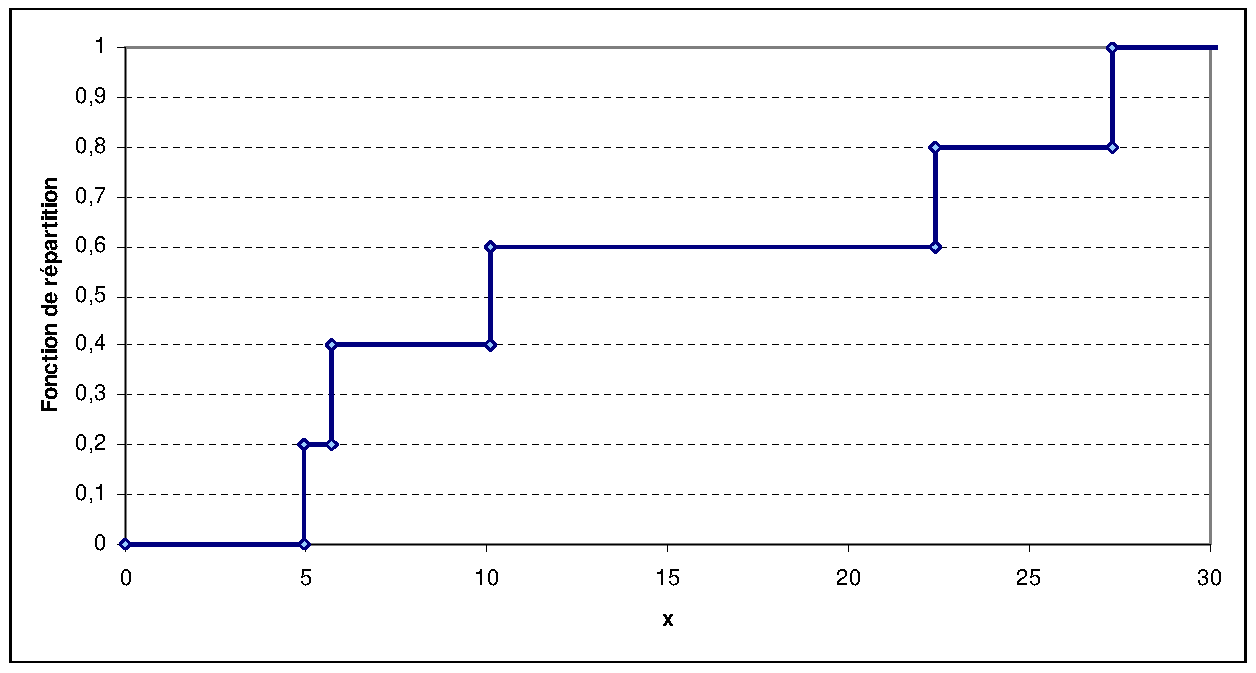
\includegraphics[scale=0.5]{foncrep.pdf}
  \end{center}
  \vspace{2mm}

  \underline{\textbf{Principle of the method for $\boldsymbol{n_X > 1}$}} \vspace{2mm}

  The method is similar for the case $n_X>1$. The empirical probability distribution is a distribution created from a sample $\left\{\vect{x}_1, \vect{x}_2, \ldots, \vect{x}_N\right\}$. It corresponds to a discrete uniform distribution on $\left\{\vect{x}_1, \vect{x}_2, \ldots, \vect{x}_N\right\}$~: where $\vect{X}'$ follows this distribution,
  $$
  \forall \; i \in \left\{1,\ldots, N\right\} ,\ \textrm{Pr}\left(\vect{X}'=\vect{x}_i\right) = \frac{1}{N}
  $$
  Thus we have:
  $$
  F_N(\vect{x}) = \frac{1}{N} \sum_{i=1}^N \mathbf{1}_{ \left\{ x^1_i \leq x^1,\ldots,x^{n_X}_N \leq x^{n_X} \right\} }
  $$
  in comparison with the theoretical probability density function $F_X$:
  $$
  F_X(x) = \Prob{X^1 \leq x^1,\ldots,X^{n_X} \leq x^{n_X}}
  $$
}
{
  This method is also referred to in the literature as the empirical distribution function.
}

\Methodology{
  This method is used in step B "Quantifying Sources of Uncertainty". It enables us to obtain a representation of the distribution of the vector $\vect{X}$ of uncertain variables defined in step A "Specifying Criteria and the Case Study", without applying any a priori modelling hypotheses.
}
{
  This method has the advantage of depending only on the observed values, without any other modelling assumptions (as in the \otref{docref_B11_KernelSmoothing}{kernel smoothing method}). Nevertheless, in the case where little data is available, the estimation of the criteria defined in step A can be less precise with this non-parametric method than with a parametric approach (e.g. the models described in \otref{docref_B121_DistributionSelection}{standard parametric models}).

  The following bibliographical references provide main starting points for further study of this method:
  \begin{itemize}
  \item Saporta G. (1990). "Probabilit�s, Analyse de donn�es et Statistique", Technip
  \item Dixon W.J. \& Massey F.J. (1983) "Introduction to statistical analysis (4th ed.)", McGraw-Hill
  \end{itemize}
}

\newpage
% Copyright (c)  2005-2010 EDF-EADS-PHIMECA.
% Permission is granted to copy, distribute and/or modify this document
% under the terms of the GNU Free Documentation License, Version 1.2
% or any later version published by the Free Software Foundation;
% with no Invariant Sections, no Front-Cover Texts, and no Back-Cover
% Texts.  A copy of the license is included in the section entitled "GNU
% Free Documentation License".
\renewcommand{\etapemethodo}{B}
\renewcommand{\nomfichier}{docref_B11_KernelSmoothing}
\renewcommand{\titrefiche}{Kernel Smoothing}

\Header

\MathematicalDescription{

  Kernel smoothing is a non parametric estimation method of the probability density function of a distribution. \\
  In dimension 1, the kernel smoothed probability density function $\hat{p}$ has the following expression, where $K$ is the univariate kernel, $n$ the numerical sample size and $(X_1, \cdots, X_n) \in \mathbb{R}^n$ the univariate random sample with $\forall i, \, \, X_i \in \mathbb{R}$ :
  \begin{equation}
    \label{kernelSmooth}
    \hat{p}(x) = \displaystyle \frac{1}{nh}\sum_{i=1}^{n} K\left(\frac{x-X_i}{h}\right)
  \end{equation}
  The kernel $K$ is a function satisfying $\int K(x)\, dx=1$. Usually, $K$ is chosen to be a unimodal probability density fucntion that is symmetric about 0.\\
  The parameter $h$ is called the \emph{bandwidth}.\\


  In dimension $d>1$, the kernel may be defined as a product kernel $K_d$, as follows where $\vect{x} = (x_1, \cdots, x_d)\in \mathbb{R}^d$  :
  $$
  K_d(\vect{x}) = \displaystyle \prod_{j=1}^{j=d} K(x_j)
  $$
  which leads to the kernel smoothed probability density function in dimension $d$, where $(\vect{X}_1, \cdots, \vect{X}_n)$ is the d-variate random  sample which components are denoted $\vect{X}_i = (X_{i1}, \dots, X_{id})$ :
  $$
  \hat{p}(\vect{x}) = \displaystyle \frac{1}{N \prod_{j=1}^{j=d}h_j} \sum_{i=1}^{N} K_d\left(\frac{x_1 - X_{i1} }{h_1}, \dots, \frac{x_d - X_{id}}{h_d}\right)
  $$
  Let's note that the bandwidth is the vector $\vect{h} = (h_1, \cdots, h_d)$. \\

  The quality of the approximation may be controlled by the AMISE (Asymptotic Mean Integrated Square error) criteria defined as :
  $$
  \left\{
    \begin{array}{lcl}
      AMISE(\hat{p}) & = & \mbox{two first terms in the series expansion with respect to $n$ in } MISE(\hat{p}) \\
      MISE(\hat{p}) & = & \mathbb{E}_\vect{X}[||\hat{p} - p||^2_{L_2}]   =  \int \, MSE(\hat{p}, \vect{x}) \, d\vect{x}  \\
      MSE(\hat{p}, \vect{x})&  =  & \left[ \mathbb{E}_\vect{X}[\hat{p}(\vect{x})] - p(\vect{x})\right]^2 + Var_\vect{X}(\hat{p}(\vect{x}))
    \end{array}
  \right.
  $$


  The quality of the estimation essentially depends on the value of the bandwidth $h$. The bandwidth that minimizes the AMISE criteria  has the expression (given in dimension 1) :
  \begin{equation}
    \label{AMISE1}
    h_{AMISE}(K) = \displaystyle \left[ \frac{R(K)}{\mu_2(K)^2R(p^{(2)})}\right]^{\frac{1}{5}}n^{-\frac{1}{5}}
  \end{equation}
  where  $R(K) = \int K(\vect{x})^2\, d\vect{x}$ and $\mu_2(K) = \int \vect{x}^2K(\vect{x})\, d\vect{x} = \sigma_K^2$.\\
  If we note that $R(p^{(r)}) = (-1)^r\Phi_{2r}$ with $\Phi_r = \int p^{(r)}p(x)\, dx = \mathbb{E}_\vect{X}[p^{(r)}]$, then relation (\ref{AMISE1}) writes :
  \begin{equation}
    \label{AMISE}
    h_{AMISE}(K) = \displaystyle \left[ \frac{R(K)}{\mu_2(K)^2\Phi_4}\right]^{\frac{1}{5}}n^{-\frac{1}{5}}
  \end{equation}

  Several rules exist to  evaluate the optimal bandwidth $ h_{AMISE}(K)$ : all efforts are concentrated on the evaluation of the term $\Phi_4$. We give here the most usual rules :
  \begin{itemize}
  \item the \emph{Silverman rule} in dimension 1,
  \item the plug-in bandwidth selection - \emph{Solve-the-equation} method in dimension $d$,
  \item the \emph{Scott rule} in dimension d.
  \end{itemize}



  \vspace*{0.5cm}
  \textbf{Silverman rule (dimension 1)}\\

  In the case where the density $p$ is normal with standard deviation $\sigma$, then the term $\Phi_4$ can be exactly evaluated. In that particular case,  the optimal bandwidth of relation (\ref{AMISE}) with respect to the AMISE criteria writes as follows :
  \begin{equation}
    \label{pNormal}
    h^{p = normal}_{AMISE}(K) = \displaystyle \left[ \frac{8\sqrt{\pi} R(K)}{3\mu_2(K)^2}\right]^{\frac{1}{5}}\sigma n^{-\frac{1}{5}}
  \end{equation}

  An estimator of $h^{p= normal}_{AMISE}(K)$ is obtained by replacing $\sigma$ by its estimator $\hat{\sigma}^n$,  evaluated from the  numerical sample $(X_1, \dots, X_n)$ :
  \begin{equation}
    \label{Estimpnormal}
    \hat{h}^{p = normal}_{AMISE}(K) = \displaystyle \left[ \frac{8\sqrt{\pi} R(K)}{3\mu_2(K)^2}\right]^{\frac{1}{5}}\hat{\sigma}^n n^{-\frac{1}{5}}
  \end{equation}

  The Silverman rule consists in considering $\hat{h}^{p = normal}_{AMISE}(K)$ of relation (\ref{Estimpnormal}) even if the density $p$ is not normal :
  \begin{equation}
    \label{Silverman}
    h^{Silver}(K) = \displaystyle \left[ \frac{8\sqrt{\pi} R(K)}{3\mu_2(K)^2}\right]^{\frac{1}{5}}\hat{\sigma}^n n^{-\frac{1}{5}}
  \end{equation}

  Relation (\ref{Silverman}) is empirical and gives good results when the density is not \emph{far} from a normal one.




  \vspace*{0.5cm}

  \textbf{Plug-in bandwidth selection - \emph{Solve-the-equation} method (dimension 1)}\\



  Relation (\ref{AMISE}) requires the evaluation of the quantity $\Phi_4$. As a generale rule, we use the estimator $\hat{\Phi}_r$ of $\Phi_r$ defined by :
  \begin{equation}
    \label{EstimPhir}
    \hat{\Phi}_r = \displaystyle \frac{1}{n}\sum_{i=1}^{n} \hat{p}^{(r)}(X_i)
  \end{equation}

  Derivating relation (\ref{kernelSmooth}) leads to :
  \begin{equation}
    \label{kernelSmoothDerivative}
    \hat{p}^{(r)}(x) = \displaystyle \frac{1}{nh^{r+1}}\sum_{i=1}^{n} K^{(r)}\left(\frac{x-X_i}{h}\right)
  \end{equation}
  and then the estimator $\hat{\Phi}_r(h)$ is defined as :
  \begin{equation}
    \label{EstimPhirFin}
    \hat{\Phi}_r(h) = \displaystyle \frac{1}{n^2h^{r+1}}\sum_{i=1}^{n}\sum_{j=1}^{n} K^{(r)}\left(\frac{X_i-X_j}{h}\right)
  \end{equation}
  We note that   $\hat{\Phi}_r(h)$ depends of the parameter $h$ which can be taken in order to minimize the AMSE (Asymptotic Mean  Square Error) criteria evaluated between $\Phi_r$ and  $\hat{\Phi}_r(h)$. The optimal parameter $h$ is :
  \begin{equation}
    \label{optimHamse}
    h^{(r)}_{AMSE} = \displaystyle \left(\frac{-2K^{(r)}(0)}{\mu_2(K)\Phi_{r+2}}\right)^{\frac{1}{r+3}}n^{-\frac{1}{r+3}}
  \end{equation}





  Given that preliminary results, the solve-the-equation plug-in method  proceeds as follows :
  \begin{enumerate}
  \item Relation (\ref{AMISE}) defines $h_{AMISE}(K)$ as a function of $\Phi_4$ we denote here as :
    \begin{equation}
      \label{rel1}
      h_{AMISE}(K) = t(\Phi_4)
    \end{equation}
  \item The term  $\Phi_4$ is approximated by its estimator defined in (\ref{EstimPhirFin}) evaluated with its optimal parameter $h^{(4)}_{AMSE}$ defined in (\ref{optimHamse}) :
    \begin{equation}
      \label{h4}
      h^{(4)}_{AMSE} = \displaystyle \left(\frac{-2K^{(4)}(0)}{\mu_2(K)\Phi_{6}}\right)^{\frac{1}{7}}n^{-\frac{1}{7}}
    \end{equation}
    which leads to a relation of type :
    \begin{equation}
      \label{rel2}
      \Phi_4 \simeq  \hat{\Phi}_4(h^{(4)}_{AMSE})
    \end{equation}

  \item Relations (\ref{AMISE}) and (\ref{h4}) lead to the new one :
    \begin{equation}
      \label{h4hAmise}
      h^{(4)}_{AMSE} = \displaystyle \left( \frac{-2K^{(4)}(0)\mu_2(K)\Phi_4}{R(K)\Phi_{6}}\right) ^{\frac{1}{7}}h_{AMISE}(K)^{\frac{5}{7}}
    \end{equation}

    which rewrites :
    \begin{equation}
      \label{rel3}
      h^{(4)}_{AMSE} = l(h_{AMISE}(K))
    \end{equation}

  \item Relation (\ref{h4hAmise}) depends on both terms $\Phi_4$ and $\Phi_6$ which are evaluated with their estimators defined in (\ref{EstimPhirFin}) respectively with their AMSE optimal parameters $g_1$ and $g_2$ (see relation (\ref{optimHamse})).  It leads to the expressions~:
    \begin{equation}
      \label{g12}
      \left\{
        \begin{array}{lcl}
          g_1 & = & \displaystyle \left(\frac{-2K^{(4)}(0)}{\mu_2(K)\Phi_{6}}\right)^{\frac{1}{7}}n^{-\frac{1}{7}}\\
          g_2 & = & \displaystyle \left(\frac{-2K^{(6)}(0)}{\mu_2(K)\Phi_{8}}\right)^{\frac{1}{7}}n^{-\frac{1}{9}}
        \end{array}
      \right.
    \end{equation}

  \item In order to evaluate $\Phi_6$ and $\Phi_8$, we suppose that the density $p$ is normal with a variance $\sigma^2$ which is approximated by the empirical variance of the numerical sample, which leads to :
    \begin{equation}
      \label{Phi68}
      \left\{
        \begin{array}{lcl}
          \hat{\Phi}_6 & = & \displaystyle \frac{-15}{16\sqrt{\pi}}\hat{\sigma}^{-7}\\
          \hat{\Phi}_8 & = & \displaystyle \frac{105^{\strut}}{32\sqrt{\pi}}\hat{\sigma}^{-9}
        \end{array}
      \right.
    \end{equation}
  \end{enumerate}

  Then, to resume, thanks to relations (\ref{rel1}), (\ref{rel2}), (\ref{rel3}), (\ref{g12}) and (\ref{Phi68}), the optimal bandwidth is solution of the equation :
  \begin{equation}
    \label{equhAmise}
    \boldsymbol{h_{AMISE}(K) = t \circ \hat{\Phi}_4 \circ l (h_{AMISE}(K))}
  \end{equation}





  \vspace*{0.5cm}


  \textbf{Scott rule (dimension d)}\\

  The Scott rule is a simplification of the Silverman rule generalized to the dimension $d$ which is optimal when the density $p$ is normal with independent components. In all the other cases, it gives an empirical rule that gives good result when the density $p$ is not \emph{far} from the normal one. For examples, the Scott bandwidth may appear too large when $p$ presents several maximum.\\

  The Silverman rule given in dimension 1 in relation (\ref{Silverman}) can be generalized in dimension $d$ as follows : if we suppose  that the density $p$ is normal with independent components, in dimension $d$ and that we use the normal kernel $N(0,1)$ to estimate it, then the optimal bandwidth vector $\vect{h}$ with respect to the AMISE criteria writes as follows :
  \begin{equation}
    \label{SilvermanNormalKernel}
    \vect{h}^{Silver}(N) = \left(\left(\frac{4}{d+2}\right)^{1/(d+4)}\hat{\sigma}_i^n n^{-1/(d+4)}\right)_i
  \end{equation}
  where $\hat{\sigma}_i^n$ is the standard deviation of the $i-th$ component of the sample $(\vect{X}_1, \cdots, \vect{X}_n)$, and $\sigma_K$ the standard deviation of the 1D kernel $K$.\\



  The Scott proposition is  a simplification of the Silverman rule, based on the fact that the coefficient $\left(\frac{4}{d+2}\right)^{1/(d+4)}$ remains in $[0.924, 1.059]$ when the dimension $d$ varies. Thus, Scott fixed it to $1$ :
  \begin{equation}
    \label{coefficientScott}
    \left(\frac{4}{d+2}\right)^{1/(d+4)} \simeq 1
  \end{equation}
  which leads to the simplified expression :
  \begin{equation}
    \label{SilvermanNormalKernelSimplif}
    \vect{h}^{Silver}(N) \simeq \left( \hat{\sigma}_i^n n^{-1/(d+4)}\right)_i
  \end{equation}




  Furthermore, in the general case, we have from relation (\ref{AMISE1}) :
  \begin{equation}
    \label{ChangeBandwidth}
    \frac{h_{AMISE}(K_1)}{h_{AMISE}(K_2)}=\frac{\sigma_{K_2}}{\sigma_{K_1}}\left[\frac{\sigma_{K_1}R(K_1)}{\sigma_{K_2}R(K_2)}\right]^{1/5}
  \end{equation}

  Considering that $\sigma_{K}R(K) \simeq 1$ whatever the kernel $K$,   relation (\ref{ChangeBandwidth}) simplifies in :
  \begin{equation}
    \label{SimplifiedChangeBandwidth}
    h_{AMISE}(K_1) \simeq h_{AMISE}(K_2)\frac{\sigma_{K_2}}{\sigma_{K_1}}
  \end{equation}





  If we consider the normal kernel $N(0,1)$ for $K_2$, then relation (\ref{SimplifiedChangeBandwidth}) writes in a more general notation :
  \begin{equation}
    \label{SimplifiedChangeBandwidthNormal}
    h_{AMISE}(K) \simeq h_{AMISE}(N)\frac{1}{\sigma_{K}}
  \end{equation}

  If $h_{AMISE}(N)$ is evaluated with the Silverman rule, (\ref{SimplifiedChangeBandwidthNormal}) rewrites :
  \begin{equation}
    \label{SimplifiedChangeBandwidthSilvNormal}
    h^{Silver}(K) \simeq h^{Silver}(N)\frac{1}{\sigma_{K}}
  \end{equation}



  At last, from relation (\ref{SilvermanNormalKernelSimplif}) and (\ref{SimplifiedChangeBandwidthSilvNormal}) applied in each direction $i$, we deduce the Scott rule :
  \begin{equation}
    \label{ScottRule}
    \boldsymbol{\vect{h}^{Scott} = \left(\frac{\hat{\sigma}_i^n}{\sigma_K}n^{-1/(d+4)}\right)_i}
  \end{equation}




  \vspace*{0.5cm}

  \textbf{Boundary treatment}\\


  In dimension 1, the boundary effects may be taken into account in Open TURNS : the boundaries are automatically detected from the numerical sample (with the $min$ and $max$ functions) and the kernel smoothed PDF is corrected in the boundary areas to remain within the boundaries, according to the miroring technique :
  \begin{itemize}
  \item the Scott bandwidth is evaluated from the numerical sample : $h$
  \item two subsamples are extracted from the inital numerical sample, containing all the points within the range $[min, min + h[$ and  $]max-h, max]$,
  \item both subsamples are transformed into their symmetric samples with respect their respective boundary : its results two samples within the range  $]min-h, min]$ and  $[max, max+h[$,
  \item a kernel smoothed PDF is built from the new numerical sample composed with the initial one and the two new ones, with the previous bandwidth $h$,
  \item this last kernel smoothed PDF is truncated within the inital range  $[min, max]$ (conditionnal PDF).
  \end{itemize}



  \vspace*{0.5cm}

  \textbf{Implementation in Open TURNS}\\
  The choice of the kind of the kernel is free in Open TURNS : it is possible to select any 1D distribution and to define it as a kernel. However, in order to optimize the efficiency of the kernel smoothing fitting (it means to minimise the AMISE error), it is recommended to select a {\bf symmetric distribution} for the kernel. \\
  All the distribution default constructors of Open TURNS create a symmetric default distribution when possible. It is also possible to work with the Epanechnikov kernel, which is a $Beta(r=2, t=4, a=-1, b=1)$. \\
  The default kernel is a product of standard Normal distribution. The dimension of the product is automatically evaluated from the random sample.\\

  The bandwidth $\vect{h}$ may be fixed by the User. However, it is recommended to let Open TURNS evaluate it automatically from the numerical sample according to the following rules :\\

  {\bf In dimension $d$}, Open TURNS automatically applies the Scott rule.\\




  {\bf In dimension 1}, the automatic bandwidth selection method depends  on the size $n$ of the numerical sample. As a matter of fact, the computation bottleneck is the estimation of the estimators $\hat{\Phi}_r$ as it requires the evaluation of a double summation on the numerical sample, which has a cost of $\mathcal{O}(n^2)$.
  \begin{itemize}
  \item if $n \leq 250$, the Solve-the-equation  plug-in method is used on the entire numerical sample. The optimal bandwidth $h_{AMISE}(N)$  is first evaluated when considering a normal kernel, resolving equation (\ref{equhAmise}) for the Normal kernel. Then relation (\ref{SimplifiedChangeBandwidthNormal}) is applied in order to evaluate $h_{AMISE}(K)$.

  \item if $n>250$, the Solve-the-equation  plug-in method is too computationnally expensive. Then, Open TURNS proceeds as follows :
    \begin{enumerate}
    \item Open TURNS evaluates the bandwidth $h^{n_1, PI}_{AMISE}(N)$ with the plug-in method applied on the first $n_1 = 250$ points of the numerical sample, using the Normal kernel $N$ (by solving equation (\ref{equhAmise}) with $K=N$);
    \item Open TURNS evaluates the bandwidth $h^{n_1, Silver}(N)$ with the Silverman rule applied on the first $n_1 = 250$ points of the numerical sample, using the Normal kernel $N$ (relation (\ref{Silverman}) with $K=N$);
    \item Open TURNS evaluates the bandwidth $h^{n, Silver}(N)$ with the Silverman rule applied on the entire numerical sample, using the Normal kernel $N$ (relation (\ref{Silverman}) with $K=N$);
    \item Considering from relation (\ref{AMISE})  that :
      \begin{equation}
        \label{fracSilvAmise}
        \displaystyle \frac{h^{Silver}(K)}{h_{AMISE}(K)} = \left[ \frac{\Phi_4(p=normal)}{\Phi_4(p)}\right]^{\frac{1}{5}}
      \end{equation}
      which is independent of the size $n$, we have the final relation :
      \begin{equation}
        \label{fracSilvAmiseFin}
        \displaystyle h^{n, PI}_{AMISE}(N) = \frac{h^{n_1, PI}_{AMISE}(N)}{h^{n_1, Silver}(N)}h^{n, Silver}(N)
      \end{equation}
      Then, if the User has chosen the kernel $K$ rather than the normal  kernel $N$, relation (\ref{SimplifiedChangeBandwidthNormal}) is used, which leads to :
      \begin{equation}
        \label{OTrule}
        \displaystyle h^{n, PI}_{AMISE}(K) = \frac{1}{\sigma_K} \frac{h^{n_1, PI}_{AMISE}(N)}{h^{n_1, Silver}_{AMISE}(N)}h^{n, Silver}_{AMISE}(N)
      \end{equation}
    \end{enumerate}
  \end{itemize}





}
{
  -
}

\Methodology{
  This kernel smoothing method can be used to estimate the probability density function :
  \begin{itemize}
  \item of the distribution of the input random variable (Step B of the global methodology),
  \item of the distribution of the ouput variable of interest (Step C of the global methodology).
  \end{itemize}


}
{


  The following references gives details on the method :
  \begin{itemize}
  \item \emph{Kernel smoothing}, M.P. Wand and M.C. Jones, Chapman \& Hall/CRC edition, ISNB 0-412-55270-1.
  \item \emph{Multivariate Density Estimation, practice and Visualisation, Theory}, David W. Scott, Wiley edition.
  \end{itemize}



}

\Example{

  \textbf{Choice of the bandwidth $h$}\\

  This example illustrates the effect of the choice of the bandwidth $h$ on the estimation of the pdf compared to the optimal one. Depending on the choice of $h$, one could observe for the same size $N$ of input values over-smoothing effects or under-smoothing effects. \\

  \textbf{\textit{Oversmoothing effect}}\\
  In this case, $h$ is bigger than the optimal choice $h_{opt}$. The effect of the values is more widely spread as in the optimal case.

  \begin{center}
    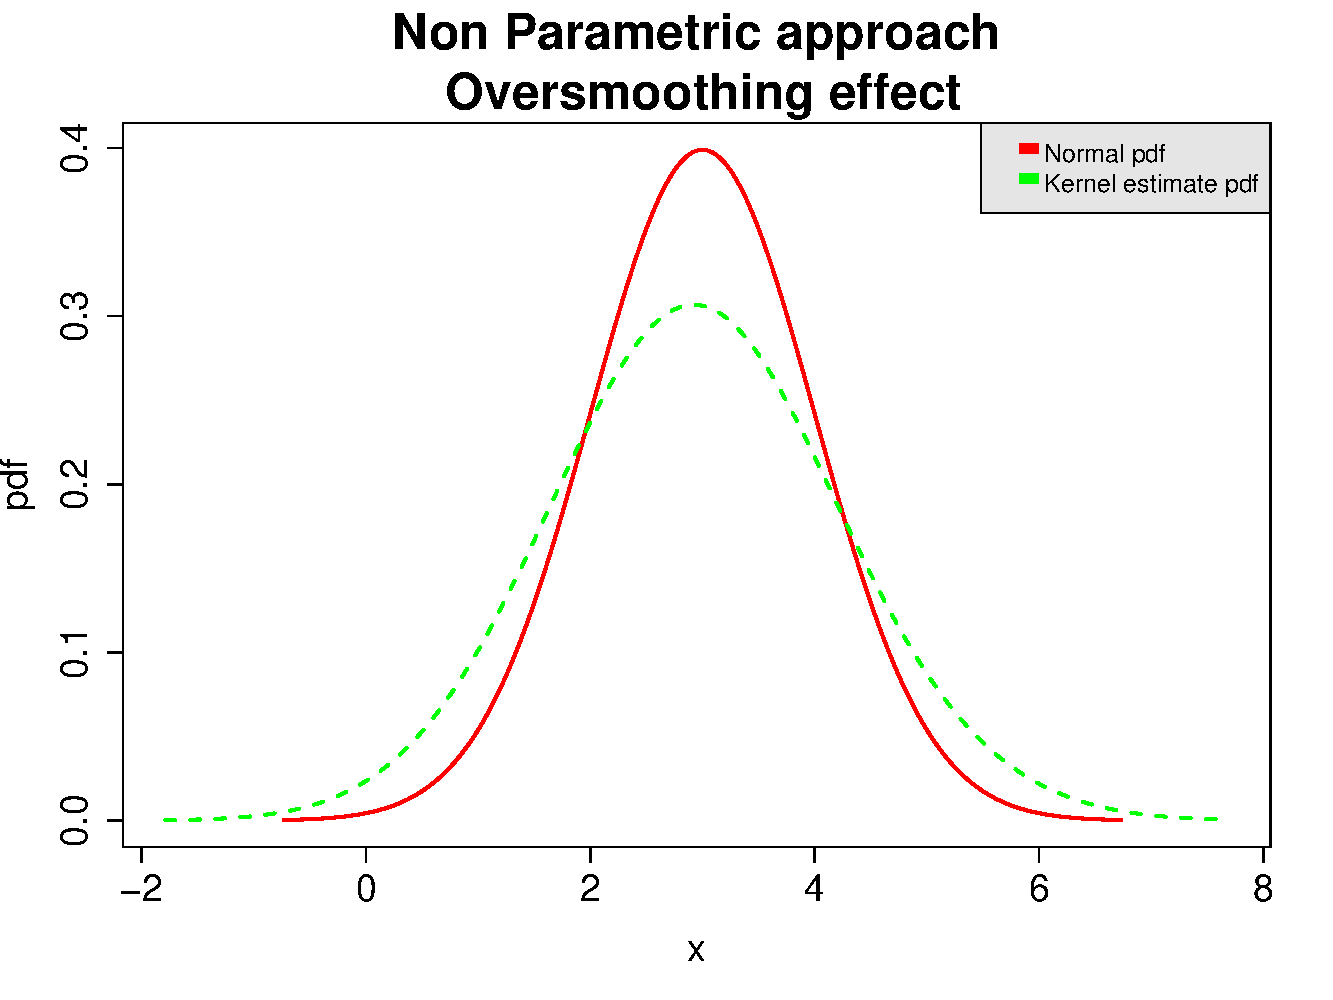
\includegraphics[width=0.50\textwidth]{oversmoothing.pdf}
  \end{center}

  \textbf{\textit{Undersmoothing effect}}\\
  In this case, $h$ is smaller than the optimal choice $h_{opt}$. The effect of the values is more locally focused on the values obtained in the data set than in the optimal case.

  \begin{center}
    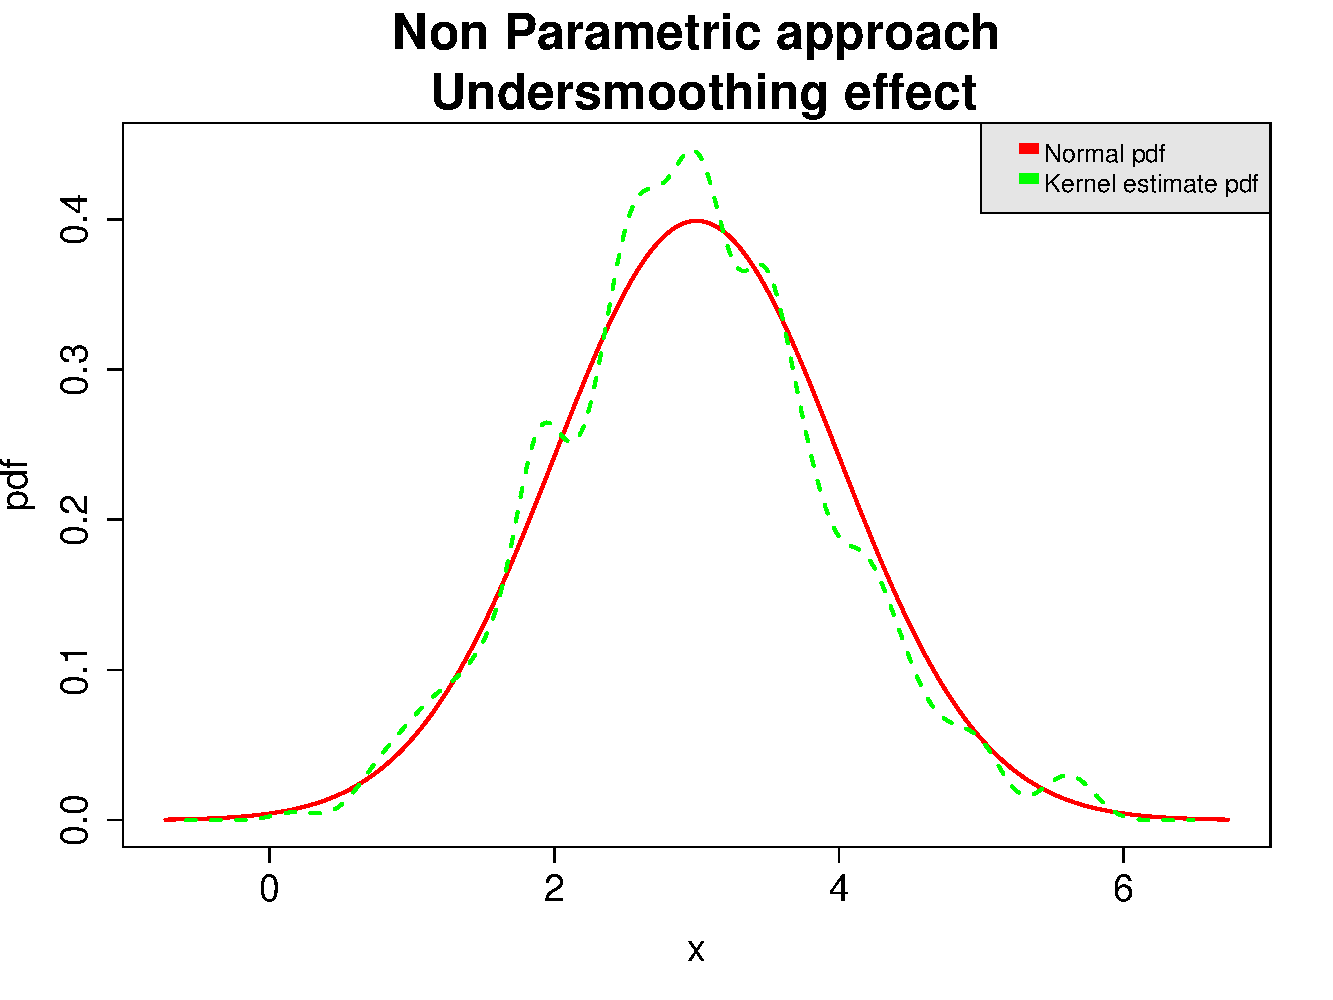
\includegraphics[width=0.60\textwidth]{undersmoothing.pdf}
  \end{center}

  \textbf{\textit{Optimal smoothing}}\\
  Following the previous Silverman rule, for a Gaussian distribution.

  \begin{center}
    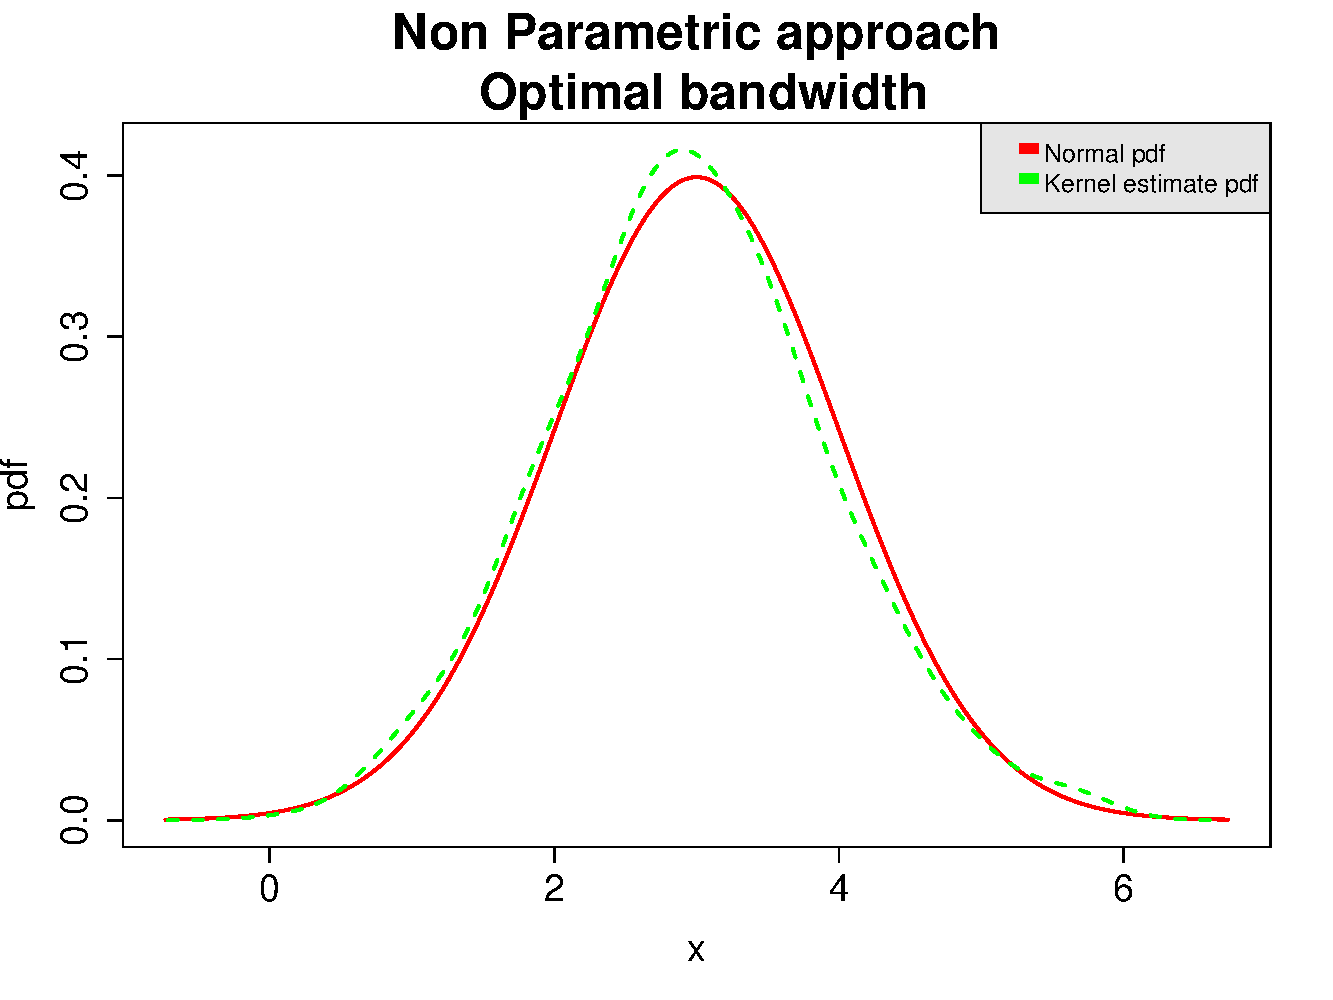
\includegraphics[width=0.50\textwidth]{OKsmoothing.pdf}
  \end{center}


}

\newpage
% Copyright (c)  2005-2010 EDF-EADS-PHIMECA.
% Permission is granted to copy, distribute and/or modify this document
% under the terms of the GNU Free Documentation License, Version 1.2
% or any later version published by the Free Software Foundation;
% with no Invariant Sections, no Front-Cover Texts, and no Back-Cover
% Texts.  A copy of the license is included in the section entitled "GNU
% Free Documentation License".
\renewcommand{\etapemethodo}{B}
\renewcommand{\nomfichier}{docref_B121_DistributionSelection}
\renewcommand{\titrefiche}{Standard parametric models}

\Header

\MathematicalDescription{

  \underline{\textbf{Objective}} \vspace{2mm}

  Parametric models aim to describe probability distributions of a random variable with the aid of a limited number of parameters $\vect{\theta}$. Therefore, in the case of continuous variables (i.e. where all possible values are continuous), this means that the probability density of $\vect{X} = \left( X^1,\ldots,X^{n_X} \right)$ can be expressed as $f_X(\vect{x};\vect{\theta})$. In the case of discrete variables (i.e. those which take only discrete values), their probabilities can be described in the form $\Prob{\vect{X} = \vect{x};\vect{\theta}}$.
  \vspace{2mm}

  The available distributions of Open TURNS are listed in this section. We start with continuous distributions.

  \begin{itemize}

  \item {\bf Arcsine distribution}~: $\vect{\theta} = \left(a,b \right)$, with the constraint $a<b$. The probability density function is expressed as:

    $$\frac{1}{\pi \frac{b-a}{2} \sqrt{1-\left(\frac{x-\frac{a+b}{2} }{ \frac{b-a}{2} }\right)^{2}}}$$
    We note that a random variable that follows a Arcsine distribution as defined here takes values in the interval $[a,b]$.

    \begin{center}
      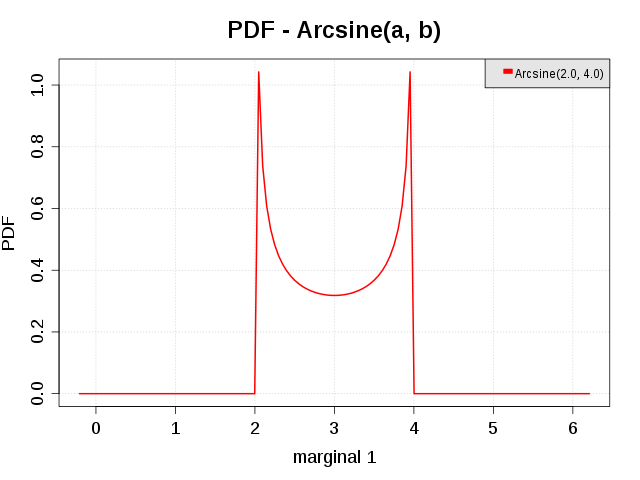
\includegraphics[scale=0.6]{pdf_Arcsine.png}
    \end{center}

  \item {\bf Beta distribution}~: Univariate distribution. $\vect{\theta} = \left( r,t,a,b \right)$, with the constraints $r>0$, $t>r$, $b>a$. The probability density function is expressed as:
    $$
    f_X(x;\vect{\theta}) = \frac{(x-a)^{r-1} (b-x)^{t-r-1}}{(b-a)^{t-1} B(r,t-r)} \mathbf{1}_{a \leq x \leq b}
    $$
    where $B$ denotes the Beta function. We note that a random variable that follows a Beta distribution as described here takes values in the interval $[a,b]$.\\
    Note that the Epanechnikov distribution is a particular Beta distribution : $Beta (a=-1, b=1, r=2, t=4)$. It is usefull within the kernel smoothing theory (see \otref{docref_B11_KernelSmoothing}{kernel smoothing}).


    \begin{figure}[H]
      \begin{minipage}{8cm}
        \begin{center}
          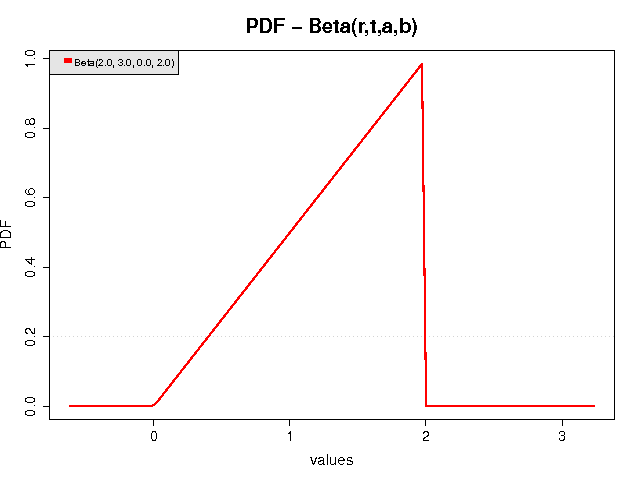
\includegraphics[width=7cm]{pdf_Beta_1.png}
          \caption{PDF of a Beta distribution.}
        \end{center}
      \end{minipage}
      \hfill
      \begin{minipage}{8cm}
        \begin{center}
          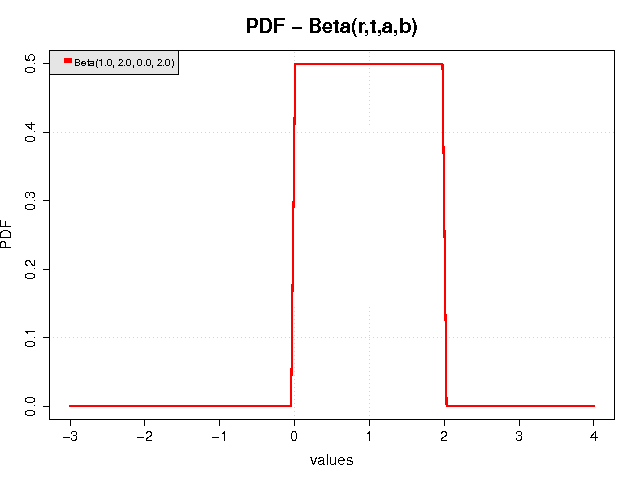
\includegraphics[width=7cm]{pdf_Beta_2.png}
          \caption{PDF of a Beta distribution.}
        \end{center}
      \end{minipage}
    \end{figure}

    \begin{figure}[H]
      \begin{minipage}{8cm}
        \begin{center}
          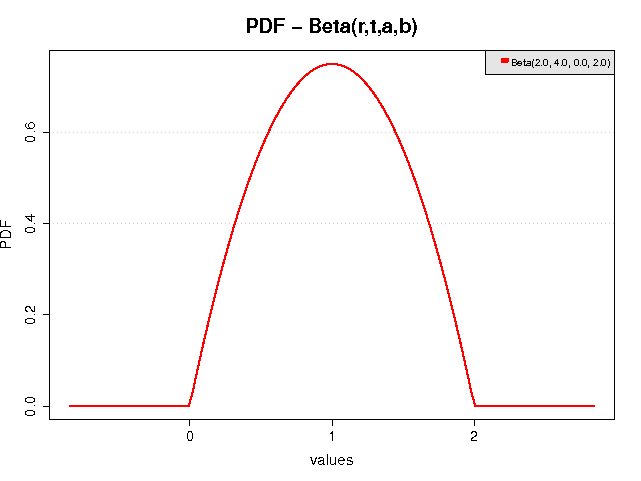
\includegraphics[width=7cm]{pdf_Beta_3.png}
          \caption{PDF of a Beta distribution.}
          % \label{PDF3}
        \end{center}
      \end{minipage}
      \hfill
      \begin{minipage}{8cm}
        \begin{center}
          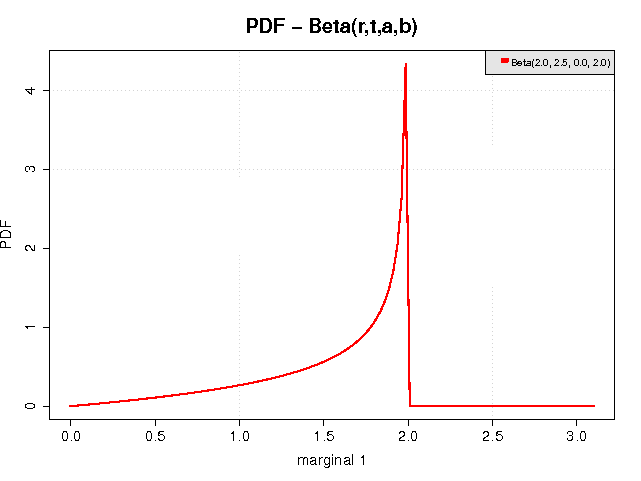
\includegraphics[width=7cm]{pdf_Beta_4.png}
          \caption{PDF of a Beta distribution.}
          % \label{PDF4}
        \end{center}
      \end{minipage}
    \end{figure}


    \begin{figure}[H]
      \begin{minipage}{8cm}
        \begin{center}
          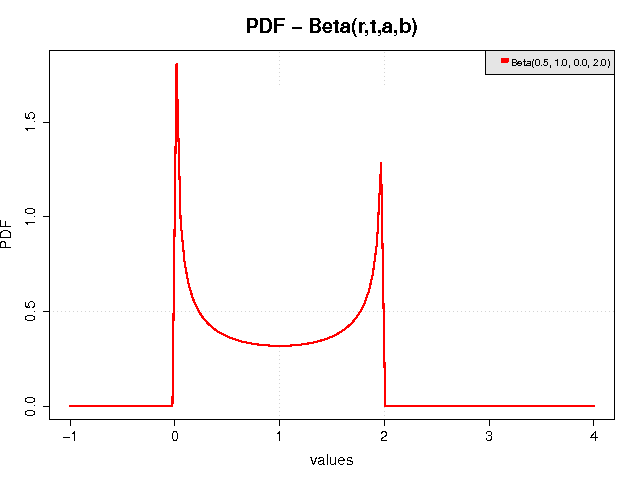
\includegraphics[width=7cm]{pdf_Beta_5.png}
          \caption{PDF of a Beta distribution.}
          % \label{PDF5}
        \end{center}
      \end{minipage}
      \hfill
      \begin{minipage}{8cm}
        \begin{center}
          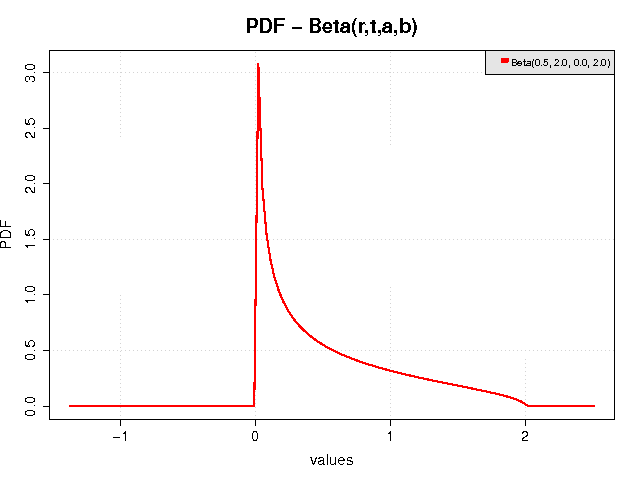
\includegraphics[width=7cm]{pdf_Beta_6.png}
          \caption{PDF of a Beta distribution.}
          % \label{PDF6}
        \end{center}
      \end{minipage}
    \end{figure}



    \begin{figure}[H]
      \begin{minipage}{8cm}
        \begin{center}
          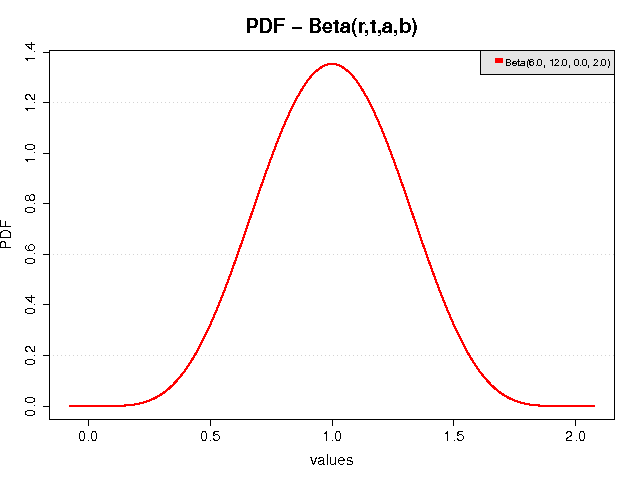
\includegraphics[width=7cm]{pdf_Beta_7.png}
          \caption{PDF of a Beta distribution.}
          % \label{PDF7}
        \end{center}
      \end{minipage}
      \hfill
      \begin{minipage}{8cm}
        \begin{center}
          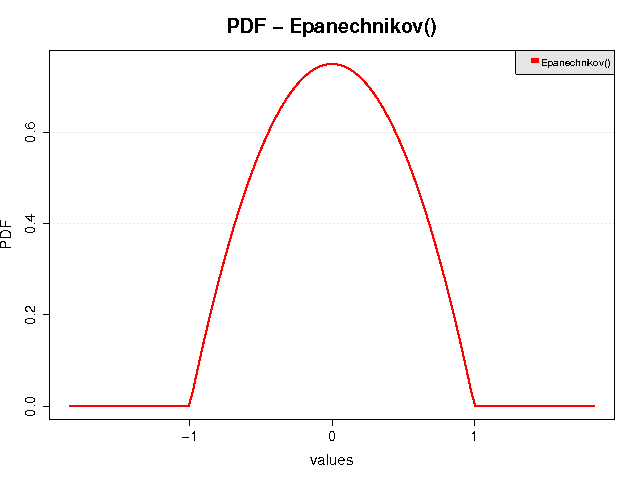
\includegraphics[width=7cm]{pdf_Epanechnikov.png}
          \caption{PDF of a Epanechnikov distribution.}
          % \label{PDF8}
        \end{center}
      \end{minipage}
    \end{figure}




  \item {\bf Burr distribution}~: Univariate distribution. $\vect{\theta} = \left( c,k \right)$, with the constraints $c>0$, $k>0$. The probability density function is expressed as:
    $$
    f_X(x;\vect{\theta}) = ck\frac{x^{(c-1)}}{(1+x^c)^{(k+1)}} \mathbf{1}_{x >0}
    $$

    \begin{figure}[H]
      \begin{minipage}{8cm}
        \begin{center}
          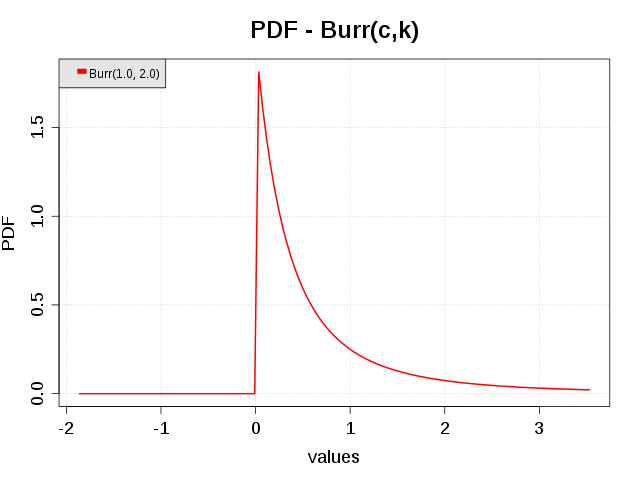
\includegraphics[width=7cm]{pdf_Burr_1.png}
          \caption{PDF of a Burr distribution.}
          % \label{PDF30}
        \end{center}
      \end{minipage}
      \hfill
      \begin{minipage}{8cm}
        \begin{center}
          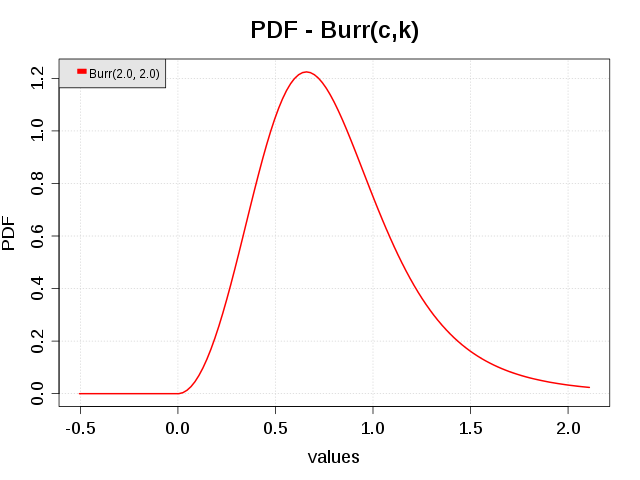
\includegraphics[width=7cm]{pdf_Burr_2.png}
          \caption{PDF of a Burr distribution.}
          % \label{PDF31}
        \end{center}
      \end{minipage}
    \end{figure}


  \item {\bf Chi}~: Univariate distribution. $\vect{\theta} = \nu$ with the constraint $\nu >0$. The probability density function is expressed as:
    $$
    f_X(x;\vect{\theta}) = \displaystyle x^{\nu-1}e^{-x^2/2}\frac{2^{1-\nu^{\strut}/2}}{\Gamma(\nu/2)_{\strut}} \boldsymbol{1}_{[0,+\infty[}(x)
    $$



    \begin{figure}[H]
      \begin{center}
        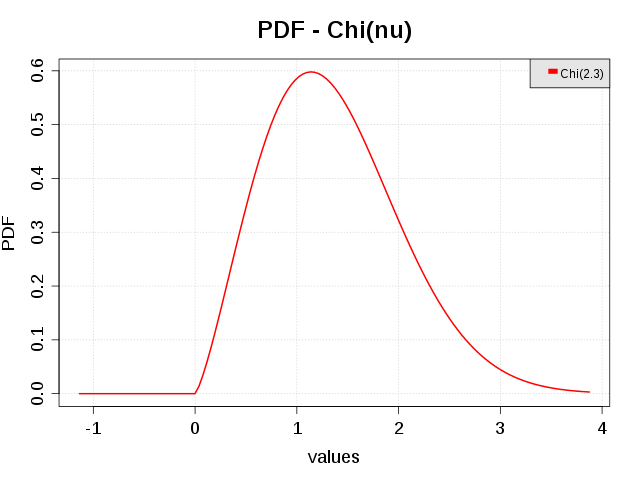
\includegraphics[width=7cm]{pdf_Chi_1.png}
        \caption{PDF of a Chi  distribution.}
        % \label{PDF11}
      \end{center}
    \end{figure}



  \item {\bf ChiSquare}~: Univariate distribution. $\vect{\theta} = \nu$ with the constraint $\nu >0$. The probability density function is expressed as:
    $$
    f_X(x;\vect{\theta}) = \displaystyle \frac{2^{-\nu^{\strut}/2}}{\Gamma(\nu/2)_{\strut}} x^{(\nu/2-1)}e^{-x/2}\boldsymbol{1}_{[0,+\infty[}(x)
    $$
    We note that a random variable which follows a ChiSquare distribution as defined here takes values in the range $[0,+\infty[$.


    \begin{figure}[H]
      \begin{minipage}{8cm}
        \begin{center}
          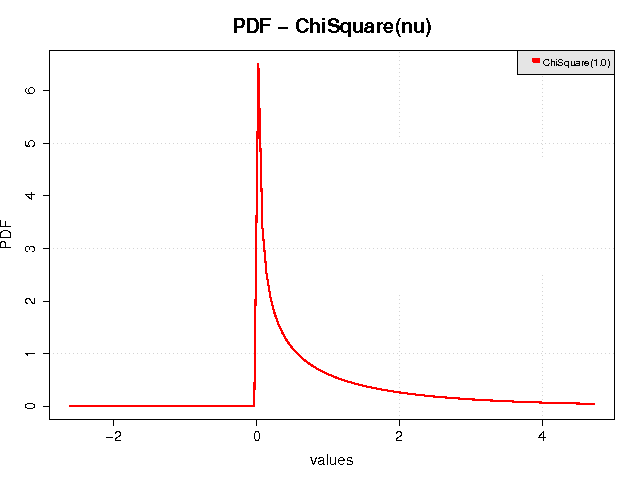
\includegraphics[width=7cm]{pdf_ChiSquare_1.png}
          \caption{PDF of a Chi Square distribution.}
          % \label{PDF9}
        \end{center}
      \end{minipage}
      \hfill
      \begin{minipage}{8cm}
        \begin{center}
          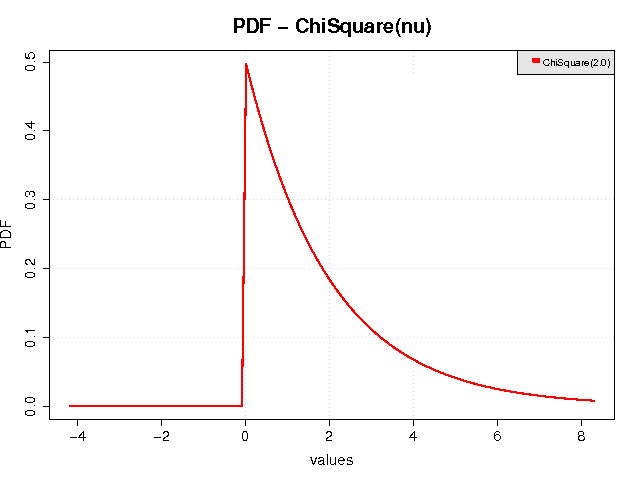
\includegraphics[width=7cm]{pdf_ChiSquare_2.png}
          \caption{PDF of a Chi Square distribution.}
          % \label{PDF10}
        \end{center}
      \end{minipage}
    \end{figure}

    \begin{figure}[H]
      \begin{center}
        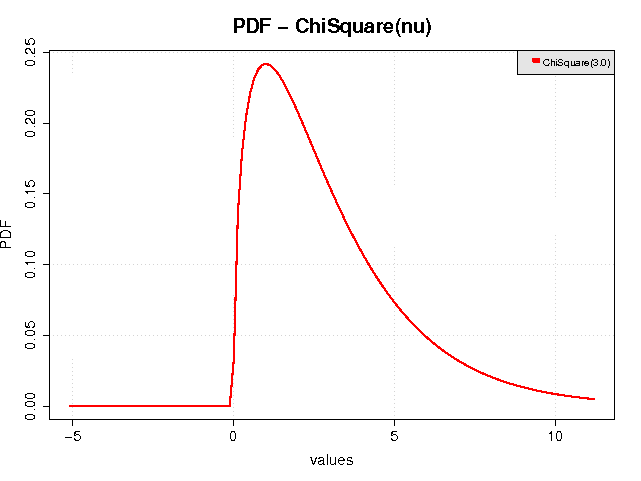
\includegraphics[width=7cm]{pdf_ChiSquare_3.png}
        \caption{PDF of a Chi Square distribution.}
        % \label{PDF11}
      \end{center}
    \end{figure}





  \item {\bf Dirichlet distribution}~: Multivariate $d$-dimensional distribution. $\vect{\theta} = ( \theta_1, \hdots, \theta_{d+1})$, with the constraints $d \geq 1$ and $\theta_i>0$. The probability density function is expressed as:
    $$
    f_X(\vect{x};\vect{\theta}) = \displaystyle \frac{\Gamma(\sum_{j=1}^{d+1}\theta_j)}{\prod_{j=1}^{d+1}\Gamma(\theta_j)} \left[ 1-\sum_{j=1}^{d} x_j\right]^{(\theta_{d+1}-1)}\prod_{j=1}^d x_j^{(\theta_j-1)}\mathbf{1}_{\Delta}(\vect{x})
    $$
    with $\Delta = \{ \vect{x} \in \mathbb{R}^d / \forall i, x_i \geq 0, \sum_{i=1}^{d} x_i \leq 1 \}$.



  \item {\bf Epanechnikov distribution}~: Univariate distribution. The Epanechnikov distribution is a particular Beta distribution : $Beta (a=-1, b=1, r=2, t=4)$. It is usefull within the kernel smoothing theory (see \otref{docref_B11_KernelSmoothing}{kernel smoothing}).


  \item {\bf Exponential distribution}~: $\vect{\theta} = \left( \lambda, \gamma \right)$, with the constraint $\lambda>0$. The probability density function is expressed as:
    $$
    f_X(x;\vect{\theta}) = \lambda \exp \left( -\lambda(x-\gamma) \right) \mathbf{1}_{\gamma \leq x}
    $$
    We note that a random variable which follows an Exponential distribution as defined here takes values in the range $[\gamma,+\infty[$, and is right skewed. Both a and � influence the dispersion. The expected value of the distribution is $\gamma + 1/\lambda$. The coefficient of variation (standard deviation / mean) is constant and equal to 1 whatever the value of $\lambda$.


    \begin{figure}[H]
      \begin{center}
        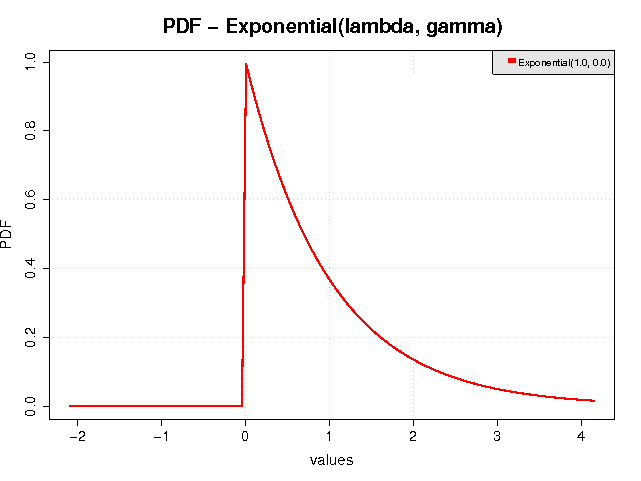
\includegraphics[width=7cm]{pdf_Exponential.png}
        \caption{PDF of a Exponential distribution.}
        % \label{PDF12}
      \end{center}
    \end{figure}


  \item {\bf Fisher-Snedecor distribution}~: $\vect{\theta} = \left(d_1, d_2 \right)$, with the constraint $d_i>0$. The probability density function is expressed as:
    $$
    f_X(x;\vect{\theta}) = \displaystyle \frac{1}{xB(d_1/2, d_2/2)}\left[\left(\frac{d_1x}{d_1x+d_2}\right)^{d_1/2} \left(1-\frac{d_1x}{d_1x+d_2}\right)^{d_2/2} \right]\mathbf{1}_{x \geq 0}
    $$
    We note that a random variable which follows an Exponential distribution as defined here takes values in the range $[\gamma,+\infty[$, and is right skewed. Both a and � influence the dispersion. The expected value of the distribution is $\gamma + 1/\lambda$. The coefficient of variation (standard deviation / mean) is constant and equal to 1 whatever the value of $\lambda$.



    \begin{figure}[H]
      \begin{minipage}{8cm}
        \begin{center}
          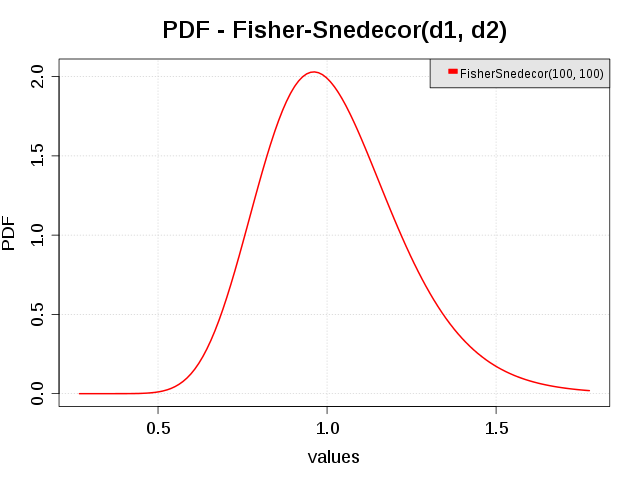
\includegraphics[width=7cm]{pdf_FisherSnedecor_1.png}
          \caption{PDF of a Fisher-Snedecor distribution.}
          % \label{PDF13}
        \end{center}
      \end{minipage}
      \hfill
      \begin{minipage}{8cm}
        \begin{center}
          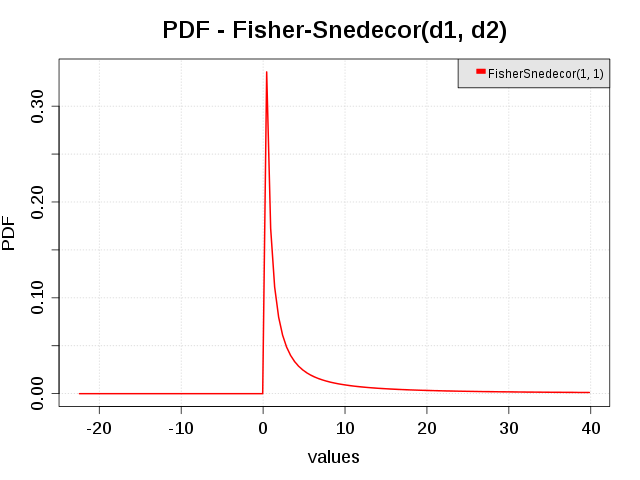
\includegraphics[width=7cm]{pdf_FisherSnedecor_2.png}
          \caption{PDF of a Fisher-Snedecor distribution.}
          % \label{PDF14}
        \end{center}
      \end{minipage}
    \end{figure}



  \item {\bf Gamma distribution}~: Univariate distribution. $\vect{\theta} = \left( \lambda, k, \gamma \right)$, with the constraints  $\lambda>0$, $k>0$. The probability density function is expressed as:
    $$
    f_X(x;\vect{\theta}) = \frac{\lambda}{\Gamma(k)} \left( \lambda(x-\gamma) \right)^{k-1} \exp \left( -\lambda(x-\gamma) \right) \mathbf{1}_{\gamma \leq x}
    $$
    where $\Gamma$ is the gamma function. We note that a random variable which follows a gamma Distribution as defined takes values in the range $[\gamma,+\infty[$, and is right skewed.


    \begin{figure}[H]
      \begin{minipage}{8cm}
        \begin{center}
          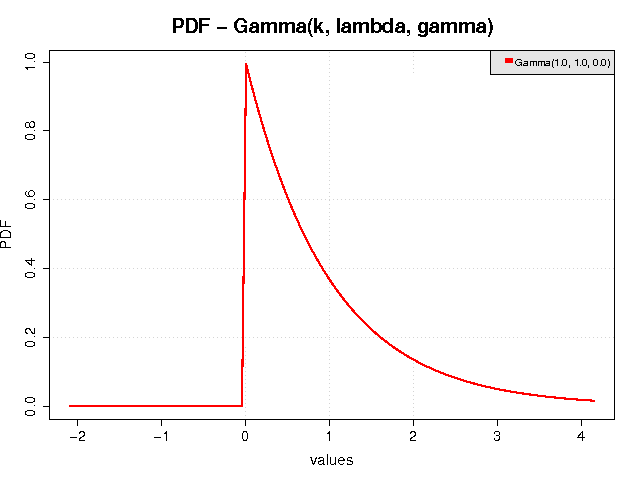
\includegraphics[width=7cm]{pdf_Gamma_1.png}
          \caption{PDF of a Gamma distribution.}
          % \label{PDF13}
        \end{center}
      \end{minipage}
      \hfill
      \begin{minipage}{8cm}
        \begin{center}
          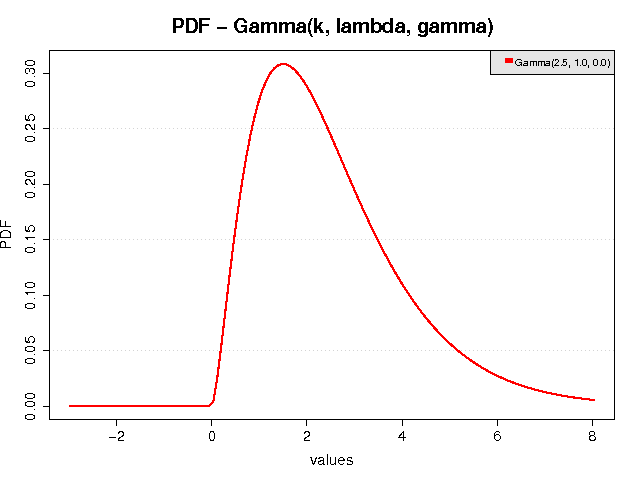
\includegraphics[width=7cm]{pdf_Gamma_2.png}
          \caption{PDF of a Gamma distribution.}
          % \label{PDF14}
        \end{center}
      \end{minipage}
    \end{figure}

    \begin{figure}[H]
      \begin{center}
        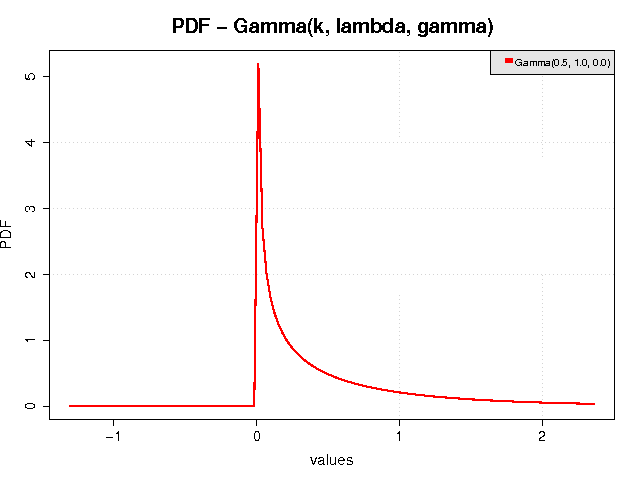
\includegraphics[width=7cm]{pdf_Gamma_3.png}
        \caption{PDF of a Gamma distribution.}
        % \label{PDF15}
      \end{center}
    \end{figure}


  \item {\bf Gumbel distribution}~: Univariate distribution. $\vect{\theta} = \left( \alpha,\beta \right)$, with the constraint $\alpha>0$. The probability density function is expressed as:
    $$
    f_X(x;\vect{\theta}) = \alpha \exp \left( -\alpha(x-\beta) - e^{-\alpha(x-\beta)} \right)
    $$

    We note that a random variable which follows a Gumbel distribution as defined here takes real values in $\mathbb{R}$. $\beta$ describes the most likely value, but this is less than the expected value of the distribution because the distribution is asymmetric (right skewed): the probability values in the distribution's right tail (i.e. values greater than $\beta$) decrease more gradually than those in the left tail (i.e. values less than $\beta$). a provides a measure of dispersion: the probability density function flattens as $\alpha$ decreases.

    \begin{figure}[H]
      \begin{center}
        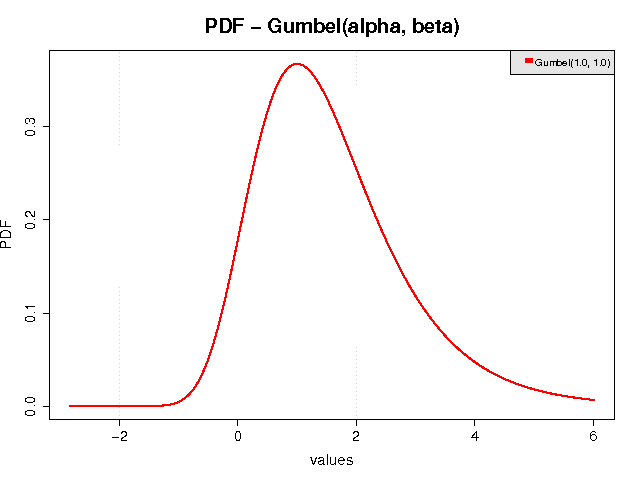
\includegraphics[width=7cm]{pdf_Gumbel.png}
        \caption{PDF of a Gumbel distribution.}
        % \label{PDF16}
      \end{center}
    \end{figure}


  \item {\bf Histogram distribution}~: Univariate distribution. $\vect{\theta} = \left( (h_i, l_i)_i \right)$, with the constraint $h_i>0$ and $l_i>0$. The probability density function is expressed as:
    $$
    f_X(x;\vect{\theta}) = \sum_{i=1}^{n}H_i\;\boldsymbol{1}_{[x_i,x_{i+1}]}(x)
    $$
    where
    \begin{itemize}
    \item $H_i=h_i/S$ is the normalized heights, with $S=\sum_{i=1}^nh_i\,l_i$ being the initial surface of the histogram.
    \item $l_i = x_{i+1} - x_i$, $1\leq i \leq n$
    \item $n$ is the size of the HistogramPairCollection
    \end{itemize}


    \begin{figure}[H]
      \begin{center}
        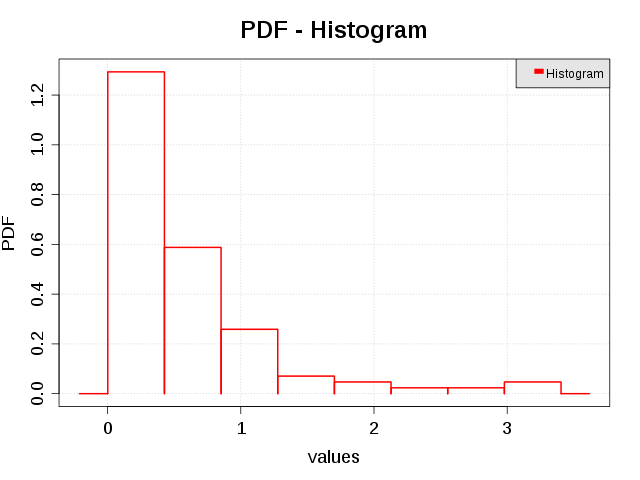
\includegraphics[width=7cm]{pdf_Histogram.png}
        \caption{PDF of a Histogram distribution.}
        % \label{PDF17}
      \end{center}
    \end{figure}



  \item {\bf Inverse Normal distribution}~: Univariate distribution. $\vect{\theta} = \left( \lambda,\mu \right)$, with the constraint $\lambda>0$ and $\mu>0$. The probability density function is expressed as:
    $$
    f_X(x;\vect{\theta}) = \displaystyle \left(\frac{\lambda}{2\pi x^3} \right)^{1/2}e^{-\lambda(x-\mu)^2/(2\mu^2x)} \mathbf{1}_{x>0}
    $$





    \begin{figure}[H]
      \begin{minipage}{8cm}
        \begin{center}
          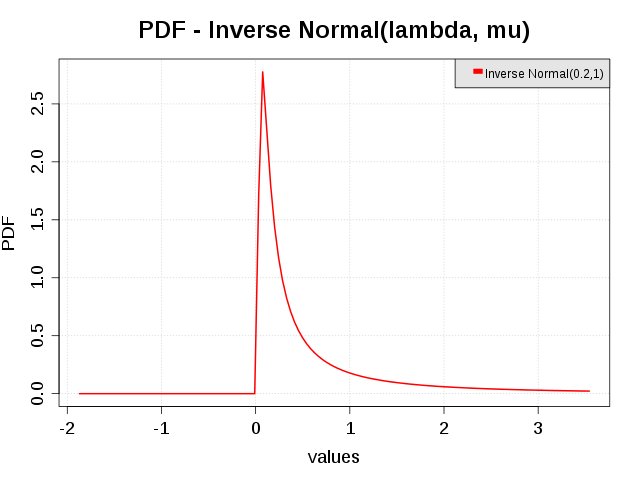
\includegraphics[width=7cm]{pdf_InverseNormal_1.png}
          \caption{PDF of a Inverse Normal distribution.}
          % \label{PDF13}
        \end{center}
      \end{minipage}
      \hfill
      \begin{minipage}{8cm}
        \begin{center}
          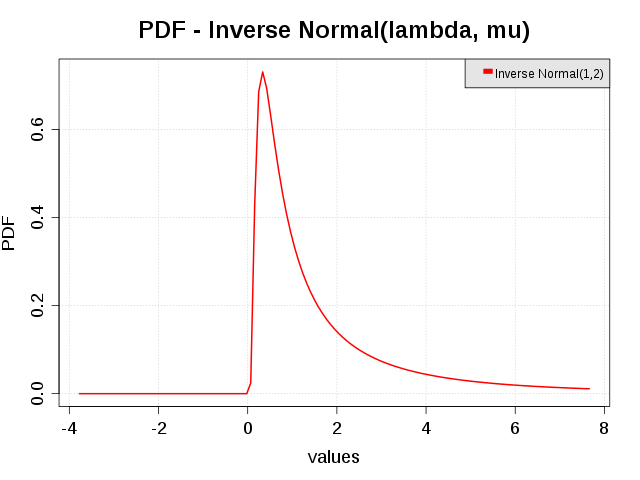
\includegraphics[width=7cm]{pdf_InverseNormal_2.png}
          \caption{PDF of a  Inverse Normal distribution.}
          % \label{PDF14}
        \end{center}
      \end{minipage}
    \end{figure}


  \item {\bf Laplace distribution}~: Univariate distribution. $\vect{\theta} = \left( \lambda, \mu \right)$, with the constraint $\lambda>0$. The probability density function is expressed as:
    $$
    f_X(x;\vect{\theta}) = \displaystyle \frac{\lambda^{\strut}}{2_{\strut}}e^{-\lambda |x-\mu|}
    $$

    The Laplace distribution is the generalisation of the Exponential distribution to the range $\mathbb{R}$.

    \begin{figure}[H]
      \begin{center}
        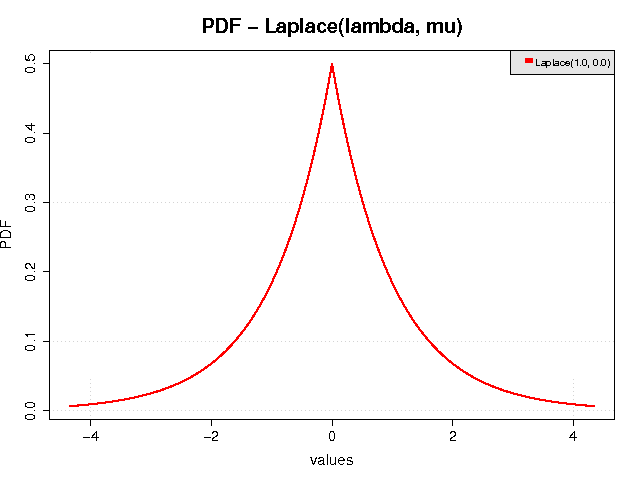
\includegraphics[width=7cm]{pdf_Laplace.png}
        \caption{PDF of a Laplace distribution.}
        % \label{PDF17}
      \end{center}
    \end{figure}





  \item {\bf Logistic distribution}~: Univariate distribution. $\vect{\theta} = \left(\alpha,\beta \right)$, with the constraint $\beta \geq 0$. The probability density function is expressed as:
    $$
    f_X(x;\vect{\theta}) = \frac{\exp \left( \frac{x-\alpha}{\beta} \right)}{\beta \left[ 1+\exp \left( \frac{x-\alpha}{\beta} \right) \right]^2}
    $$
    We note that a random variable which follows a Logistic distribution as defined here takes real values in $\mathbb{R}$. $\alpha$ describes the most likely value. $\beta$ provides a measure of dispersion: the probability density function flattens as $\beta$ decreases.

    \begin{figure}[H]
      \begin{center}
        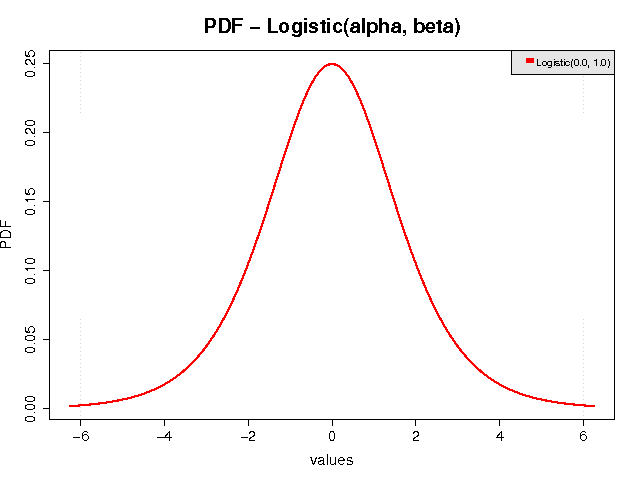
\includegraphics[width=7cm]{pdf_Logistic.png}
        \caption{PDF of a  logistic distribution.}
        % \label{PDF18}
      \end{center}
    \end{figure}


  \item {\bf Log-normal distribution}~: Univariate distribution. $\vect{\theta} = \left(\mu_\ell,\sigma_\ell,\gamma \right)$, with the constraint $\sigma_\ell>0$. The probability density function is expressed as:
    $$
    f_X(x;\vect{\theta}) = \frac{1}{\sigma_\ell (x-\gamma) \sqrt{2\pi}} \exp \left( -\frac{1}{2} \left( \frac{\textrm{ln}(x-\gamma)-\mu_\ell}{\sigma_\ell}  \right)^2 \right) \mathbf{1}_{\gamma \leq x}
    $$
    We note that a random variable which follows a Log-normal distribution as defined here takes values in the range $[\gamma,+\infty[$, and is right skewed.

    \begin{figure}[H]
      \begin{center}
        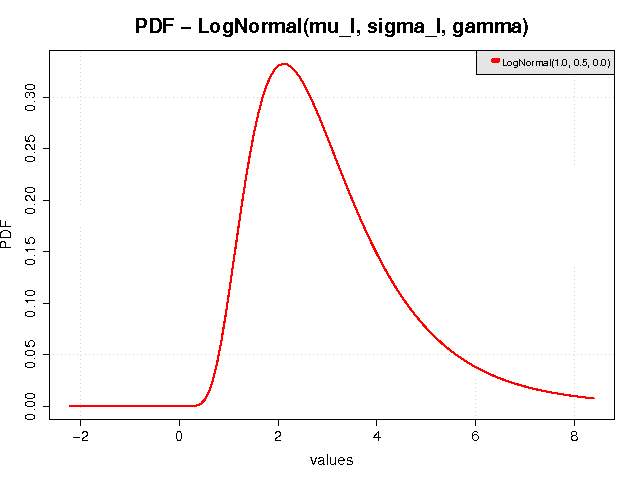
\includegraphics[width=7cm]{pdf_LogNormal.png}
        \caption{PDF of a  LogNormal distribution.}
        % \label{PDF19}
      \end{center}
    \end{figure}


  \item {\bf Log-uniform distribution}~: Univariate distribution. $\vect{\theta} = \left(a_\ell,b_\ell\right)$, with the constraint $b_\ell>a_\ell$. The probability density function is expressed as:
      $$
      f_X(x;\vect{\theta}) = \frac{1}{x(b_\ell-a_\ell)}\mathbf{1}_{a_\ell \leq \log(x) \ leq b_\ell}
      $$
      We note that a random variable which follows a Log-uniform distribution as defined here takes values in the range $[\exp(a_\ell),\exp(b_\ell)]$, and is right skewed.

      \begin{figure}[H]
        \begin{center}
          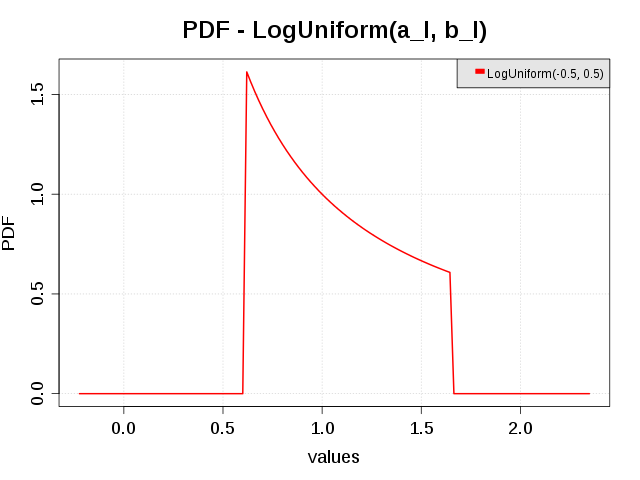
\includegraphics[width=7cm]{pdf_LogUniform.png}
          \caption{PDF of a  LogUniform distribution.}
          % \label{PDF19}
        \end{center}
      \end{figure}


    \item {\bf Non Central Chi Square}~: Univariate distribution. $\vect{\theta} = \left(\nu,\lambda \right)$, with the constraint $\nu>0$ and $\lambda\geq0$. The probability density function is expressed as:
      $$
      f_X(x;\vect{\theta}) = \displaystyle \sum_{j=0}^{\infty} e^{-\lambda}\frac{\lambda^j}{j!}p_{\chi^2(\nu+2j)}(x)
      $$
      where $p_{\chi^2(q)}$ is the probability density function of a $\chi^2(q)$ random variate.




      \begin{figure}[H]
        \begin{minipage}{8cm}
          \begin{center}
            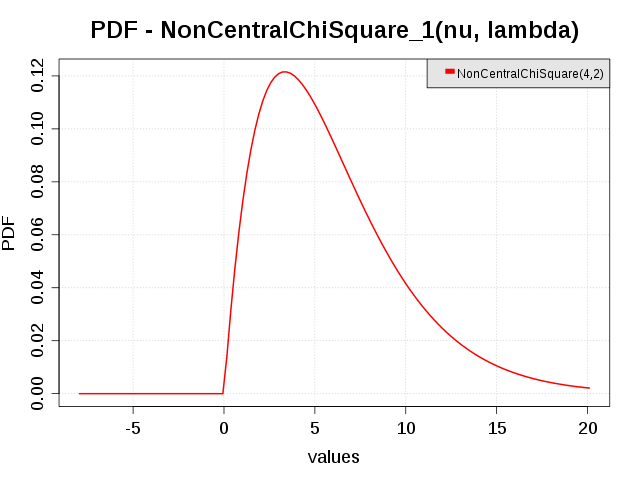
\includegraphics[width=7cm]{pdf_NonCentralChiSquare_1.png}
            \caption{PDF of a Non Central Chi Square distribution.}
            % \label{PDF13}
          \end{center}
        \end{minipage}
        \hfill
        \begin{minipage}{8cm}
          \begin{center}
            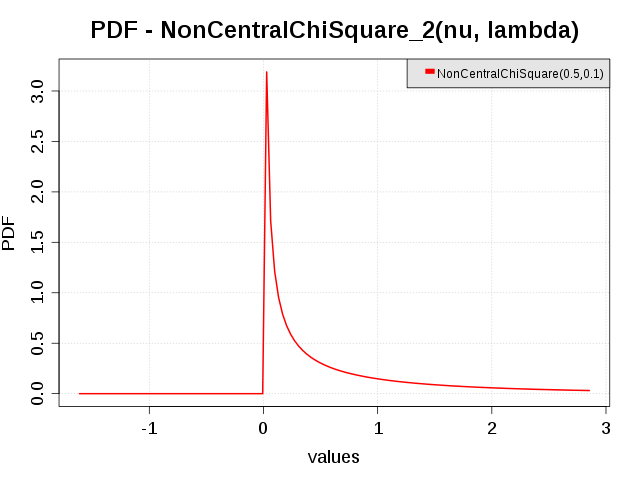
\includegraphics[width=7cm]{pdf_NonCentralChiSquare_2.png}
            \caption{PDF of a  Non Central Chi Square distribution.}
            % \label{PDF14}
          \end{center}
        \end{minipage}
      \end{figure}








    \item {\bf Non Central Student}~: Univariate distribution. $\vect{\theta} = \left(\nu,\delta, \gamma \right)$. Let's note that a random variable $X$ is said to have a standard non-central student distribution $\mathcal{T}(\nu, \delta)$ if it can be written as:
      \begin{equation}
        X = \frac{N}{\sqrt{C/\nu}}
      \end{equation}
      where $N$ has the normal distribution $\mathcal{N}(\delta, 1)$ and $C$ has the $\chi^2(\nu)$ distribution, $N$ and $C$ being independent.\\
      The non-central Student distribution in OpenTURNS has an additional parameter $\gamma$ such that the random variable $X$ is said to have a non-central Student distribution $\mathcal{T}(\nu, \delta, \gamma)$ if $X-\gamma$ has a standard $\mathcal{T}(\nu,\delta)$ distribution.\\

      We explicitate here the probability density function of the Non Central Student :
      $$
      p_{NCS}(x) = \frac{\exp(-\delta^2 / 2)}{\sqrt{\nu\pi} \Gamma(\nu / 2)}\left(\frac{\nu}{\nu + (x-\gamma)^2}\right) ^ {(\nu + 1) / 2} \sum_{j=0}^{\infty} \frac{\Gamma\left(\frac{\nu + j + 1}{2}\right)}{\Gamma(j + 1)}\left(\delta(x-\gamma)\sqrt{\frac{2}{\nu + (x-\gamma)^2}}\right) ^ j
      $$


      \begin{figure}[H]
        \begin{center}
          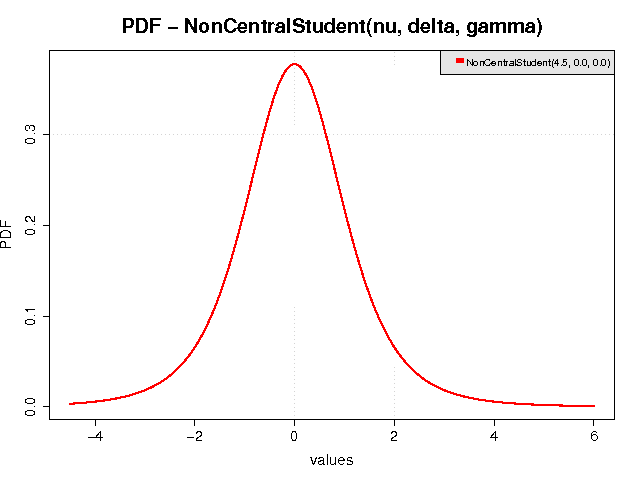
\includegraphics[width=7cm]{pdf_NonCentralStudent.png}
        \end{center}
        \caption{PDF of a Non Central Student distribution.}
        % \label{PDF19bis}
      \end{figure}





    \item {\bf Normal distribution (or Gaussian distribution)}~: Multivariate $n$-dimensional distribution. In the case $n=1$, $\vect{\theta} = \left(\mu,\sigma \right)$, with the constraint  $\sigma>0$. The probability density is given as:
      $$
      f_X(x;\vect{\theta}) = \frac{1}{\sigma \sqrt{2\pi}} \exp \left( -\frac{1}{2} \left( \frac{x-\mu}{\sigma} \right)^2 \right)
      $$
      We note that a random variable which follows a Normal distribution as defined here takes real values in $\mathbb{R}$. $\mu$ provides the most likely value (for which the probability density function is at its highest), and the density function is symmetric around this value (the values $\mu-a$ and $\mu+a$ are equally likely); $\mu$ is also the expected value (mean) of this distribution. Whilst $\sigma$ provides a measure of dispersion: the larger it is, the flatter the probability density function is (i.e. values far away from $\mu$ are still likely, or in other words possible values are more spread out).

      \begin{figure}[H]
        \begin{center}
          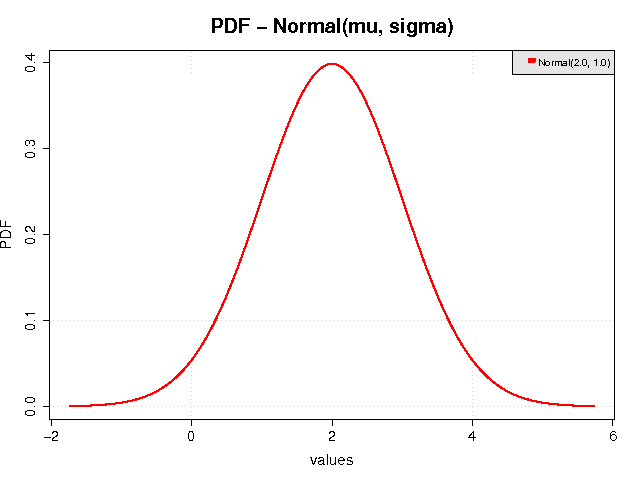
\includegraphics[width=7cm]{pdf_Normal.png}
          \caption{PDF of a Normal distribution.}
          % \label{PDF20}
        \end{center}
      \end{figure}

      In dimension $n>1$, the {\bf Multi-Normal Distribution (or Multivariate Normal Distribution)} writes :
      $$
      f_X(x;\vect{\theta}) = \displaystyle
      \frac{1}
      {
        \displaystyle (2\pi)^{\frac{n}{2}}(\mathrm{det}\mat{\Sigma})^{\frac{1}{2}}
      }
      \displaystyle e^{-\frac{1}{2}\Tr{(\vect{x}-\vect{\mu})}\mat{\Sigma}^{-1^{\strut}}(\vect{x}-\vect{\mu})}
      $$
      where  $\mat{\Sigma} = \mat{\Lambda}_{\vect{\sigma}} \mat{R} \mat{\Lambda}_{\vect{\sigma}}$, $\mat{\Lambda}_{\vect{\sigma}} = \mathrm{diag}(\vect{\sigma})$, $\mat{R}$ SPD, $\sigma_i >0$. The distribution is parameterized by  $(\vect{\mu}, \vect{\sigma},\mat{R})$ or $(\vect{\mu}, \mat{\Sigma})$.





    \item {\bf Random Mixture distribution}~:   Univariate or Multivariate $n$-dimensional distribution, dependaing on the dimension of the associated intial distributions. A Random Mixture $Y$ is defined as an affine combination of  random variables $X_i$ as follows :
      $$
      \displaystyle Y = a_0 + \sum_{i=1}^n a_i X_i
      $$
      where $(a_i)_{ 0 \leq i \leq n} \in \mathbb{R}^{n+1}$ and $(X_i)_{ 1 \leq i \leq n}$ are some independent univariate distributions.\\
      For example,   $$
      Y = 2 + 5X_1 + X_2
      $$
      where :
      \begin{itemize}
      \item  $X_1$ follows a $\mathcal{E}xponential(\lambda = 1.5)$,
      \item  $X_3$ follows a $\mathcal{N}ormal(\mu = 4,Variance = 1)$.
      \end{itemize}
      The pdf and cdf of this distribution are drawn in Fig.\ref{RMpdf} and Fig.\ref{RMcdf}.


      \begin{figure}[H]
        \begin{minipage}{8cm}
          \begin{center}
            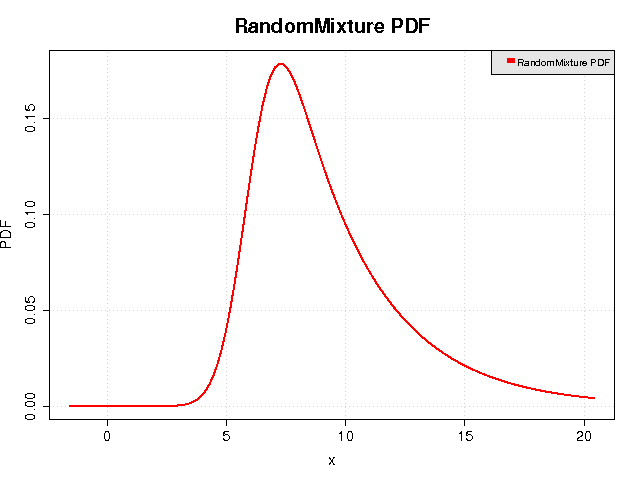
\includegraphics[width=7cm]{RandomMixture_pdf.png}
            \caption{Probability density function of a Random Mixture.}
            \label{RMpdf}
          \end{center}
        \end{minipage}
        \hfill
        \begin{minipage}{8cm}
          \begin{center}
            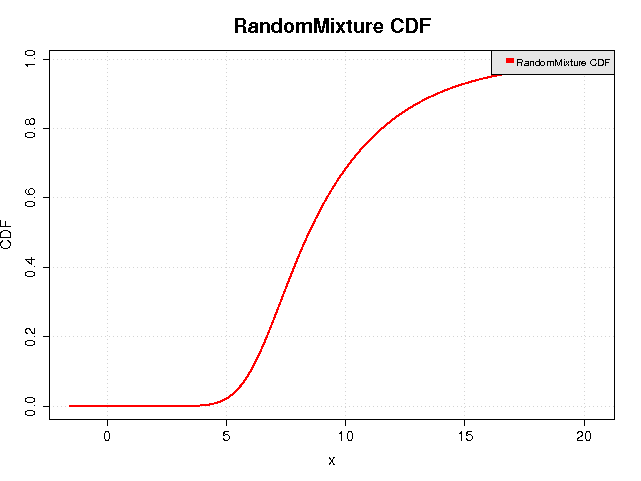
\includegraphics[width=7cm]{RandomMixture_cdf.png}
            \caption{Cumulative density function of a Random Mixture.}
            \label{RMcdf}
          \end{center}
        \end{minipage}
      \end{figure}





    \item {\bf Rice distribution}~:   Univariate distribution. $\vect{\theta} = \left( \sigma, \nu \right)$, with the constraint  $\nu\geq0$ and $\sigma>0$. The probability density is given as:
      $$
      f_X(x;\vect{\theta}) = \displaystyle 2\frac{x}{\sigma^2}p_{\chi^2(2,\frac{\nu^2}{\sigma^2})}(\frac{x^2}{\sigma^2})
      $$
      where $p_{\chi^2(\nu, \lambda)}$ is the probability density function of a Non Central Chi Square distribution.



      \begin{figure}[H]
        \begin{minipage}{8cm}
          \begin{center}
            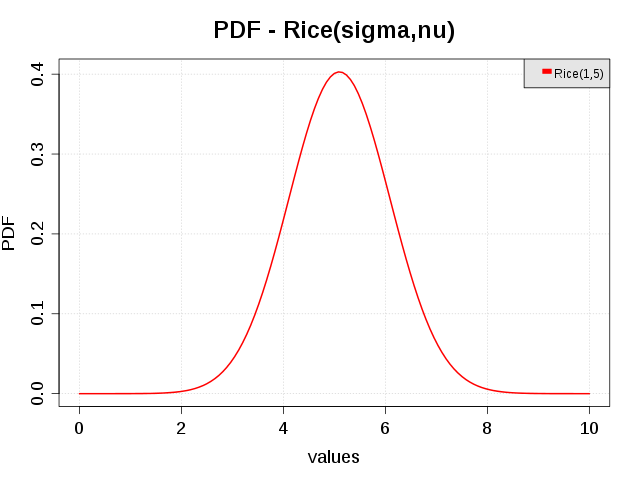
\includegraphics[width=7cm]{pdf_Rice_1.png}
            \caption{Probability density function of a Rice distribution.}
            % \label{RMpdf}
          \end{center}
        \end{minipage}
        \hfill
        \begin{minipage}{8cm}
          \begin{center}
            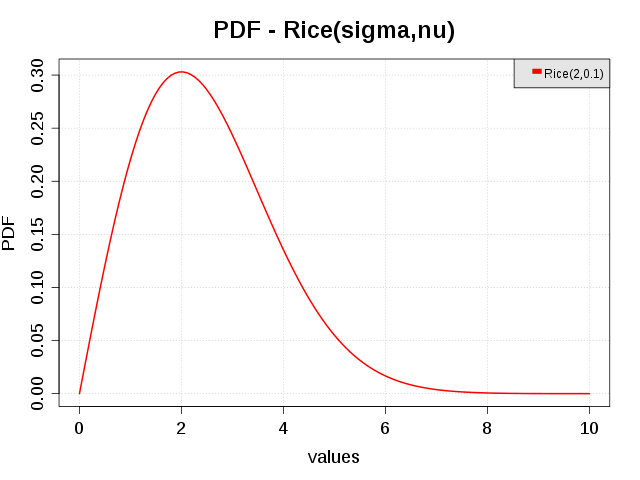
\includegraphics[width=7cm]{pdf_Rice_2.png}
            \caption{Cumulative density function of a Rice distribution.}
            % \label{RMcdf}
          \end{center}
        \end{minipage}
      \end{figure}





    \item {\bf Rayleigh distribution}~:   Univariate distribution. $\vect{\theta} = \left( \sigma, \gamma \right)$, with the constraint  $\sigma>0$.The probability density is given as:
      $$
      f_X(x;\vect{\theta}) = \displaystyle \frac{(x - \gamma)}{\sigma^2}e^{-\frac{(x-\gamma)^2}{2\sigma^2}}\boldsymbol{1}_{[\gamma,+\infty[}(x)
      $$

      \begin{figure}[H]
        \begin{center}
          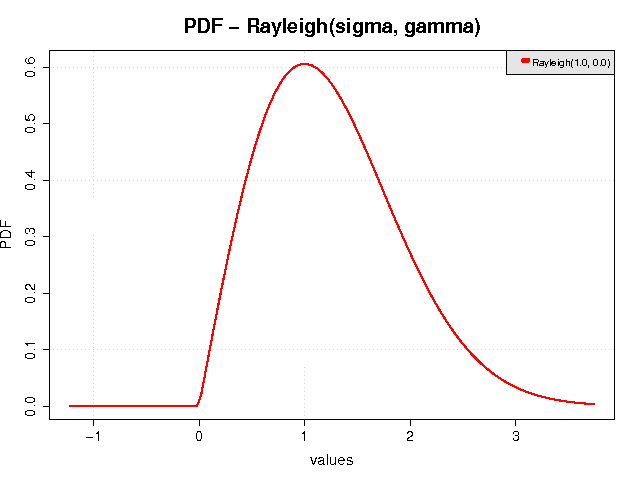
\includegraphics[width=7cm]{pdf_Rayleigh.png}
          \caption{PDF of a Rayleigh distribution.}
          % \label{PDF21}
        \end{center}
      \end{figure}






    \item {\bf Student distribution}~:  Univariate distribution. $\vect{\theta} = \left( \nu,\vect{\mu}, \vect{\sigma}, \mat{R}\right)$, with the constraint $\nu > 2$.The Student distribution has the following  probability density function, written en dimension $d$ :
      $$
      p_T(\vect{x}) = \frac{\Gamma\left(\frac{\nu+d}{2}\right)}
      {(\pi d)^{\frac{d}{2}}\Gamma\left(\frac{\nu}{2}\right)}\frac{\left|\mathrm{det}(\mat{R})\right|^{-1/2}}{\prod_{k=1}^d\sigma_k}\left(1+\frac{\vect{z}^t\mat{R}^{-1}\vect{z}}{\nu}\right)^{-\frac{\nu+d}{2}}
      $$
      where $\vect{z}=\mat{\Delta}^{-1}\left(\vect{x}-\vect{\mu}\right)$ with $\mat{\Delta}=\mat{\mathrm{diag}}(\vect{\sigma})$.\\

      In dimension $d=1$, $\vect{\theta} = (\nu, \mu, \sigma)$ and the distribution writes :
      $$
      \displaystyle p_T(x) = \frac{\Gamma\left(\frac{\nu+1}{2}\right)}
      {\sqrt{\pi}\Gamma\left(\frac{\nu}{2}\right)}\frac{1}{\sigma}\left(1+\frac{(x-\mu)^2}{\nu}\right)^{-\frac{\nu+1}{2}}
      $$
      The parameter $\mu$ describes the most likely value. $\nu$ is a measure of dispersion: the probability density function flattens as $\nu$ decreases.

      \begin{figure}[H]
        \begin{center}
          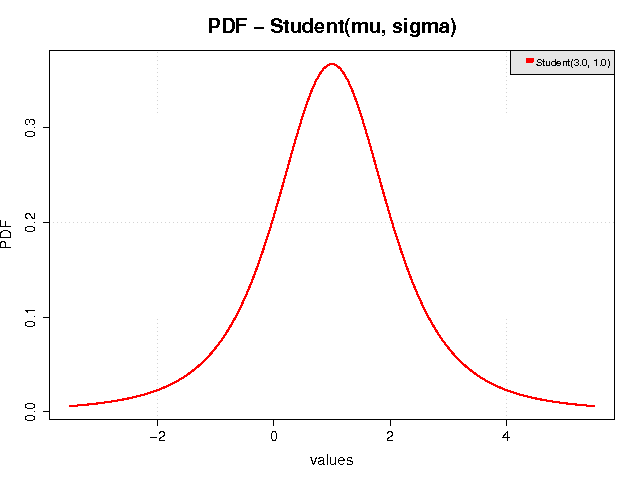
\includegraphics[width=7cm]{pdf_Student.png}
          \caption{PDF of a Student distribution.}
          % \label{PDF22}
        \end{center}
      \end{figure}

    \item {\bf Trapezoidal distribution}~: $\vect{\theta} = \left(a,b,c,d \right)$, with the constraint $a \leq b < c \leq d$. The probability density function is expressed as:
      $$
      f_X(x;\vect{\theta}) = \left\{
        \begin{array}{ll}
          h \frac {x-a}{b-a} & \textrm{if}\ a\leq x \leq b \\
          h & \textrm{if}\ b\leq x \leq c \\
          h \frac{d-x}{d-c}& \textrm{if}\ c\leq x \leq d \\
          0 & \textrm{otherwise}
        \end{array}
      \right.
      $$
      with
      $h=\frac{2}{d+c-a-b}$\\
      We note that a random variable that follows a Trapezoidal distribution as defined here takes values in the interval $[a,d]$.

      \begin{center}
        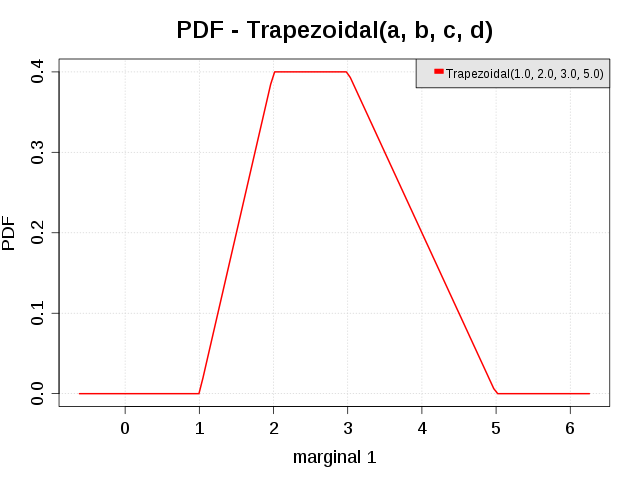
\includegraphics[scale=0.6]{pdf_Trapezoidal.png}
      \end{center}


    \item {\bf Triangular distribution}~: Univariate distribution. $\vect{\theta} = \left(a,b,m \right)$, with the constraints $a \leq m$, $m \leq b$, $b>a$. The probability density function is expressed as:
      $$
      f_X(x;\vect{\theta}) = \left\{
        \begin{array}{ll}
          2 \frac{x-a}{(m-a)(b-a)} & \textrm{if}\ a\leq x \leq m \\
          2 \frac{b-x}{(b-m)(b-a)} & \textrm{if}\ m\leq x \leq b \\
          0 & \textrm{otherwise}
        \end{array}
      \right.
      $$
      We note that a random variable that follows a triangular distribution as defined here takes in the interval $[a,b]$. $m$ describes the most likely value.

      \begin{figure}[H]
        \begin{center}
          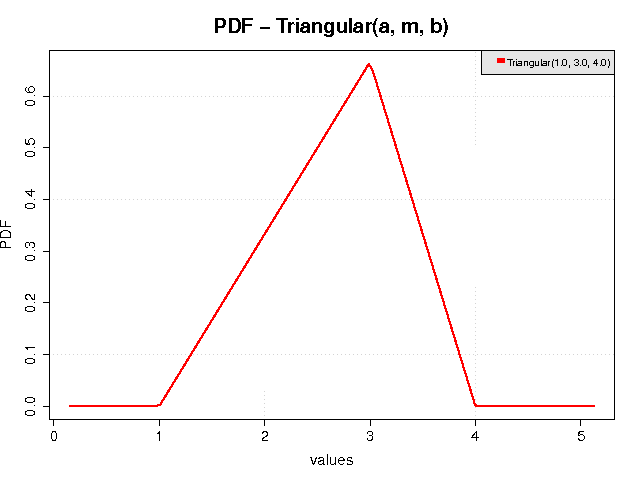
\includegraphics[width=7cm]{pdf_Triangular.png}
          \caption{PDF of a  Triangular distribution.}
          % \label{PDF23}
        \end{center}
      \end{figure}



    \item {\bf Truncated Normal Distribution}~: Univariate distribution. $\vect{\theta} = \left(\mu_n,\sigma_n,a,b \right)$, with the constraints $\sigma_n>0$, $b>a$. The probability density function is expressed as:
      $$
      f_X(x;\vect{\theta}) = \frac{\varphi(\frac{x-\mu_n}{\sigma_n}) / \sigma_n}{\Phi(\frac{b-\mu_n}{\sigma_n})-\Phi(\frac{a-\mu_n}{\sigma_n})} \mathbf{1}_{a \leq x \leq b}
      $$
      where $\varphi$ and $\Phi$ represent the probability density and the cumulative distribution function respectively of the reduced centred Normal distribution (i.e. the mean $\mu$ zero and standard deviation $\sigma$ equal to 1). We note that a random variable that follows a Truncated Normal Distribution takes values in the interval $[a,b]$. $\mu$ describes the most likely value. Whilst $\sigma$ provides a measure of dispersion: the probability density function flattens as s increases (the probability density becomes zero for values outside the interval $[a,b]$).

      \begin{figure}[H]
        \begin{minipage}{8cm}
          \begin{center}
            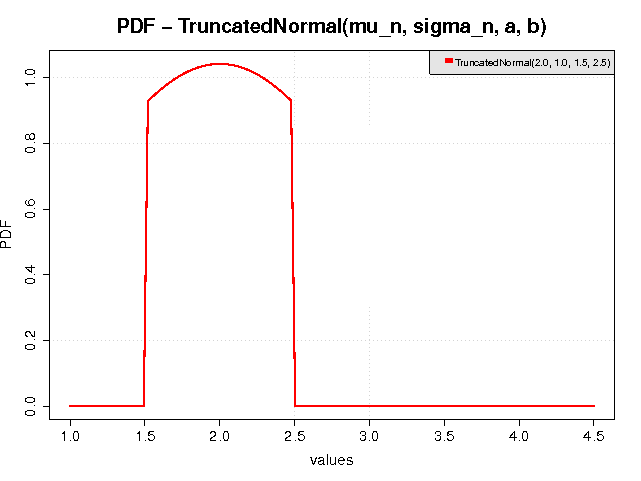
\includegraphics[width=7cm]{pdf_TruncatedNormal_1.png}
            \caption{PDF of a  TruncatedNormal distribution.}
            % \label{PDF24}
          \end{center}
        \end{minipage}
        \hfill
        \begin{minipage}{8cm}
          \begin{center}
            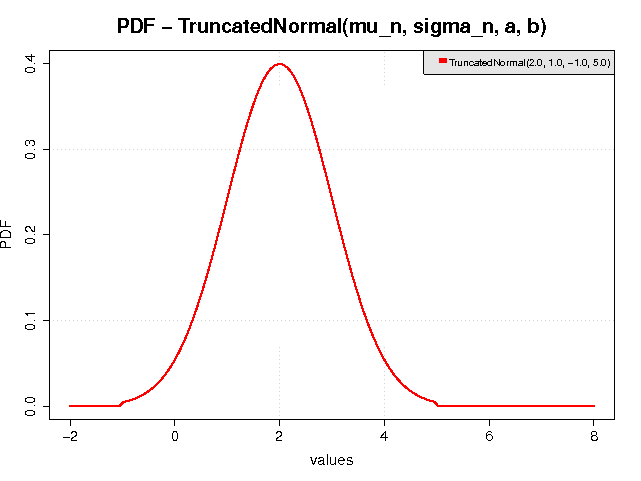
\includegraphics[width=7cm]{pdf_TruncatedNormal_2.png}
            \caption{PDF of a  TruncatedNormal distribution.}
            % \label{PDF25}
          \end{center}
        \end{minipage}
      \end{figure}




    \item {\bf Uniform distribution}~: Univariate distribution.  $\vect{\theta} = \left(a,b \right)$, with the constraint $a < b$. The probability density function is expressed as:
      $$
      f_X(x;\vect{\theta}) = \frac{1}{b-a} \mathbf{1}_{a \leq x \leq b}
      $$
      We note that a random variable that follows a uniform distribution as defined here takes values in the interval $[a,b]$. All values in this interval are equally-likely.

      \begin{figure}[H]
        \begin{center}
          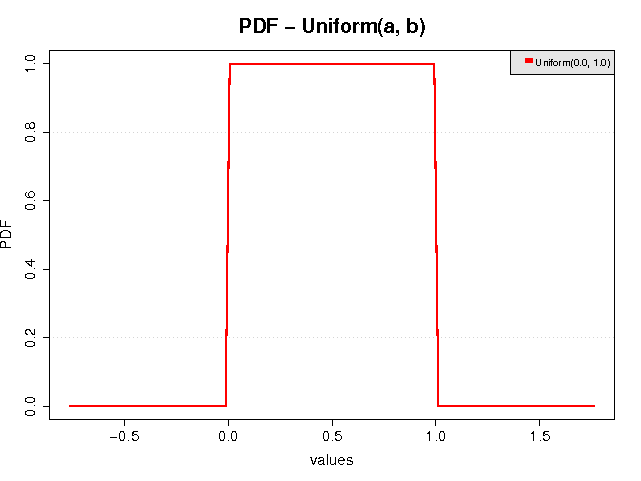
\includegraphics[width=7cm]{pdf_Uniform.png}
          \caption{PDF of a  Uniform distribution.}
          % \label{PDF26}
        \end{center}
      \end{figure}





    \item {\bf Weibull distribution}~: Univariate distribution. $\vect{\theta} = \left( \alpha,\beta, \gamma \right)$, with the constraints $\alpha>0$, $\beta>0$. probability density function is expressed as:
      $$
      f_X(x;\vect{\theta}) = \frac{\beta}{\alpha} \left( \frac{x-\gamma}{\alpha} \right)^{\beta-1} \exp \left( -\left( \frac{x-\gamma}{\alpha} \right)^\beta \right) \mathbf{1}_{\gamma \leq x}
      $$
      We note that a random variable which follows a Weibull distribution as defined here takes values in the range $[\gamma,+\infty[$, and is right skewed. Both $\alpha$ and $\beta$ influence the dispersion. We note that the distribution becomes more skewed as $\beta$ decreases. In the case where $\beta = 1$ this is corresponds to the Exponential distribution.

      \begin{figure}[H]
        \begin{minipage}{8cm}
          \begin{center}
            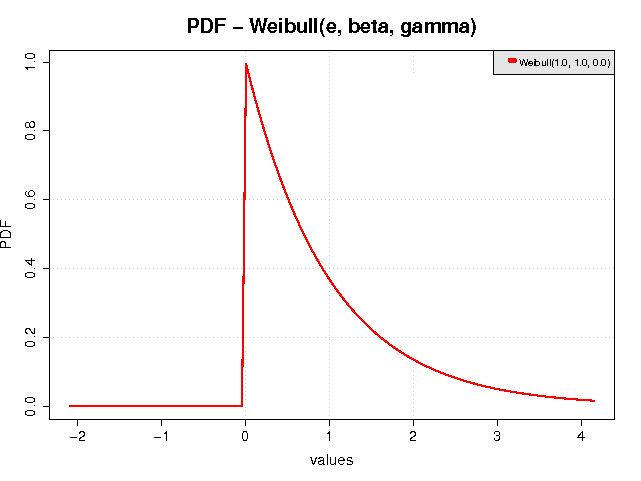
\includegraphics[width=7cm]{pdf_Weibull_1.png}
            \caption{PDF of a  Weibull distribution.}
            % \label{PDF27}
          \end{center}
        \end{minipage}
        \hfill
        \begin{minipage}{8cm}
          \begin{center}
            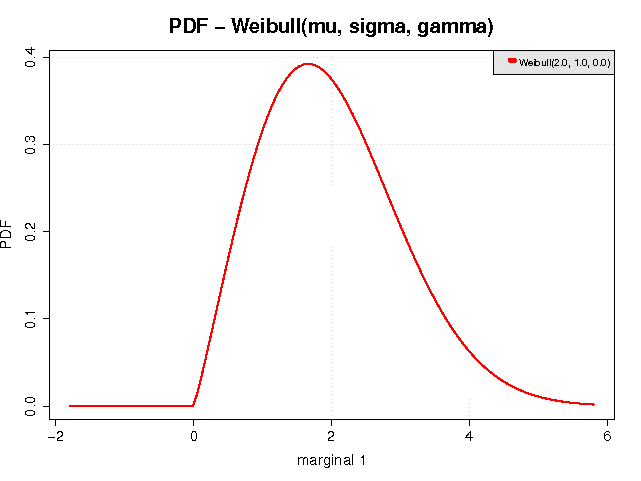
\includegraphics[width=7cm]{pdf_Weibull_2.png}
            \caption{PDF of a Weibull distribution.}
            % \label{PDF28}
          \end{center}
        \end{minipage}
      \end{figure}



    \end{itemize}



    Open TURNS also proposes some Discrete Distributions.

    \begin{itemize}

    \item {\bf Bernoulli distribution}~: Univariate distribution. $\vect{\theta} = p$, with the constraint $0<p<1$. The Bernoulli distribution takes only 2 values : 0 and 1.
      $$
      \Prob{X = 1} = p, \, \Prob{X = 0} = 1-p
      $$

      \begin{figure}[H]
        \begin{minipage}{8cm}
          \begin{center}
            \includegraphics[width=7cm]{pdf_Bernoulli.png}
            \caption{Distribution of a Bernoulli distribution.}
            \label{PDFBernoulli}
          \end{center}
        \end{minipage}
        \hfill
        \begin{minipage}{8cm}
          \begin{center}
            \includegraphics[width=7cm]{cdf_Bernoulli.png}
            \caption{CDF of a Bernoulli distribution.}
            \label{CDFBernoulli}
          \end{center}
        \end{minipage}
      \end{figure}

    \item {\bf Binomial distribution}~: Univariate distribution. $\vect{\theta} = (n,p)$, with the constraint $0<p<1$ and . The Binomial distribution values are the integer between 0 and n.
      $$
      \displaystyle P(X = k) = C_n^k p^k (1-p)^{{n-k}}
      $$
      where
      $$
      \begin{array}{@{}l@{}}
        k^{\strut} \in \{0, \hdots, n\} \\
        n \in \mathbb{N} \\
        p \in [0,1]
      \end{array}
      $$



      \begin{figure}[H]
        \begin{minipage}{8cm}
          \begin{center}
            \includegraphics[width=7cm]{pdf_Binomial.png}
            \caption{Distribution of a Binomial distribution.}
            \label{PDFBinomial}
          \end{center}
        \end{minipage}
        \hfill
        \begin{minipage}{8cm}
          \begin{center}
            \includegraphics[width=7cm]{cdf_Binomial.png}
            \caption{CDF of a Binomial distribution.}
            \label{CDFBinomial}
          \end{center}
        \end{minipage}
      \end{figure}





    \item {\bf Geometric distribution}~: Univariate distribution. $\vect{\theta} = p$, with the constraint $0<p<1$. all natural numbers $k \in \mathbb{N}^*$,
      $$
      \Prob{X = k ; \vect{\theta}} = p \left(1-p\right)^{k-1}
      $$
      We note that a random variable that follows a Geometric Distribution as defined here takes values in $\mathbb{N}^*$.

      \begin{figure}[H]
        \begin{minipage}{8cm}
          \begin{center}
            \includegraphics[width=7cm]{pdf_Geometric.png}
            \caption{Distribution of a Geometric distribution.}
            \label{PDFGeometric}
          \end{center}
        \end{minipage}
        \hfill
        \begin{minipage}{8cm}
          \begin{center}
            \includegraphics[width=7cm]{cdf_Geometric.png}
            \caption{CDF of a Geometric distribution.}
            \label{CDFGeometric}
          \end{center}
        \end{minipage}
      \end{figure}




    \item {\bf Multinomial distribution}~: Multivariate $n$-dimensional distribution. $\vect{\theta} = ((p_k)_{1 \leq k \leq n}, N)$, with the constraint $0<p<1$ and $x_i \in \mathbb{N}^*$,
      $$
      \displaystyle P(\vect{X} = \vect{x}) = \frac{N!}{x_1!\dots x_n! (N-s)!}p_1^{x_1}\dots p_n^{x_n}(1-q)^{N-s}
      $$
      where
      $$
      \begin{array}{@{}l@{}}
        0^{\strut}\leq p_i \leq 1 \\
        x_i\in \mathbb{N} \\
        \displaystyle q = \sum_{k=1}^n p_k \leq 1 \\
        s=  \sum_{k=1}^n x_k \leq N_{\strut}
      \end{array}
      $$
      In dimension $n=1$, this definition corresponds to the Binomial distribution.





    \item {\bf Poisson distribution}~: Univariate distribution. $\vect{\theta} = \lambda$, with the constraint $\lambda > 0$. For all $k \in \mathbb{N}$,
      $$
      \Prob{X = k ; \vect{\theta}} = \frac{\lambda^k}{k!} \exp \left( -\lambda \right)
      $$

      We note that a random variable that follows a Poisson distribution as defined here takes values in $\mathbb{N}$.


      \begin{figure}[H]
        \begin{minipage}{8cm}
          \begin{center}
            \includegraphics[width=7cm]{pdf_Poisson.png}
            \caption{Distribution of a Poisson distribution.}
            \label{PDFPoisson}
          \end{center}
        \end{minipage}
        \hfill
        \begin{minipage}{8cm}
          \begin{center}
            \includegraphics[width=7cm]{cdf_Poisson.png}
            \caption{CDF of a Poisson distribution.}
            \label{CDFPoisson}
          \end{center}
        \end{minipage}
      \end{figure}


    \item {\bf UserDefined}~:  Multivariate $n$-dimensional distribution. $\vect{\theta} = (\vect{x_k}, p_k)_{1 \leq k \leq N}$, with the constraint $\lambda > 0$, where $0\leq p_k \leq 1$, $\displaystyle \sum_{k=1}^{N^{\strut}} p_k = 1$.
      $$
      P(\vect{X} = \vect{x}_k) = p_k)_{1 \leq k \leq N}
      $$

      We note that a random variable that follows a Poisson distribution as defined here takes values in $\mathbb{N}$.


      \begin{figure}[H]
        \begin{minipage}{8cm}
          \begin{center}
            \includegraphics[width=7cm]{pdf_UserDefined.png}
            \caption{Distribution of a  UserDefined distribution.}
            \label{PDFUserDefined}
          \end{center}
        \end{minipage}
        \hfill
        \begin{minipage}{8cm}
          \begin{center}
            \includegraphics[width=7cm]{cdf_UserDefined.png}
            \caption{CDF of a UserDefined distribution.}
            \label{CDFUserDefined}
          \end{center}
        \end{minipage}
      \end{figure}



    \item {\bf Zipf-Mandelbrot distribution}~: Univariate distribution. $\vect{\theta} = \left( N,q,s \right)$, with the constraints $N \geq 1$, $q \geq 0$ and $s>0$. For all $k \in [1,N]$, $k$ integer,
      $$
      \forall k\in [1,N], P(X=k) = \frac{1}{(k+q)^s} \frac{1}{H(N,q,s)}
      $$
      where $H(N,q,s)$ is the Generalized Harmonic Number : $H(N,q,s) = \sum_{i=1}^{N} \displaystyle \frac{1}{(i+q)^s}$.

      \begin{figure}[H]
        \begin{minipage}{8cm}
          \begin{center}
            \includegraphics[width=7cm]{pdf_ZipfMandelbrot_1.png}
            \caption{Distribution of a  Zipf-Mandelbrot distribution.}
            \label{PDFZipfMandelbrot}
          \end{center}
        \end{minipage}
        \hfill
        \begin{minipage}{8cm}
          \begin{center}
            \includegraphics[width=7cm]{cdf_ZipfMandelbrot_1.png}
            \caption{CDF of a Zipf-Mandelbrot  distribution.}
            \label{CDFZipfMandelbrot}
          \end{center}
        \end{minipage}
      \end{figure}



    \end{itemize}

  }

  \Methodology{
    These probability distributions can be used in step B "Quantifying Sources of Uncertainty". Choosing a probability distribution is equivalent to implicitly making a hypothesis on the type of uncertainty of one of the variables $\vect{X}$ defined in step A "Specifying Criteria and the Case Study".
  }
  {
    This parametric approach has the advantage of characterizing the uncertainty using a reduced number of parameters. This is particularly useful when there is little data available for the unknown variables (situation in which a non-parametric approach would be limited -- see \otref{docref_B11_EmpiricalCDF}{empirical distribution function} and \otref{docref_B11_KernelSmoothing}{kernel smoothing}) and even when there is no data (the analysis can thus only rely on expert judgement, easier to interpret when there are few distribution parameters). \vspace{2mm}

    Moreover, a parametric approach is often preferable when the uncertainty study criterion defined in step A is concerned with a rare event, obtaining a precise evaluation of the necessary criteria generally necessitates the extrapolation of X values from the observed data. Beware however! An unwise modelling assumption (bad choice of distribution) can lead to an erroneous extrapolation and thus the results of the study may be false! \vspace{2mm}

    The correct choice of probability distribution is thus crucial. Statistical tools are available to validate or invalidate the choice of distribution given a set of data (see for example \otref{docref_B221_Graph}{Graphical analysis} \otref{docref_B222_TestKS}{Kolmogorov-Smirnov test}). But consideration of the underlying context is also recommended. For example:
    \begin{itemize}
    \item    the Normal distribution is relevant in metrology to represent certain measures of uncertainty.
    \item    the Exponential distribution is useful for modelling uncertainty when considering the life duration of material that is not subject to ageing,
    \item    the Gumbel distribution is defined to describe extreme phenomenon (e.g. maximal annual flow of a river or of wind speed)
    \end{itemize}
    \vspace{2mm}

    Some distributions are often used to express expert judgement in simple terms:
    \begin{itemize}
    \item the Uniform distribution expresses knowledge concerning the absolute limits of variables (i.e. the probability to exceed these limits is strictly zero) without any other prior assumption about the distribution (such as, for example the mean value or the most likely value),
    \item the Triangular distribution expresses knowledge concerning the absolute limits of variables and the most likely value.
    \end{itemize}

    Finally, an important point concerning the multi-dimensional case where $n_X > 1$. Choosing the type of distribution implies an assumption about the uncertainty of each of the variables $X^i$, but also on the potential inter-dependencies between variables. These inter-dependencies between unknown variables can consequently have an impact on the results of the uncertainty study.

    Readers wishing to consider the dependencies in their study more deeply are referred to, for example, \otref{docref_B122_Copulas}{copula method}, \otref{docref_B231_Pearson}{linear correlation}, \otref{docref_B232_Spearman}{rank correlation}. \vspace{2mm}

    The following bibliographical references provide main starting points for further study of this method:
    \begin{itemize}
    \item Saporta, G. (1990). "Probabilit�s, Analyse de donn�es et Statistique", Technip
    \item Dixon, W.J. \& Massey, F.J. (1983) "Introduction to statistical analysis (4th ed.)", McGraw-Hill
      % \item NIST/SEMATECH e-Handbook of Statistical Methods, http://www.itl.nist.gov/div898/handbook/
      % \item D'Agostino, R.B. and Stephens, M.A. (1986). "Goodness-of-Fit Techniques", Marcel Dekker, Inc., New York.
    \item Bhattacharyya, G.K., and R.A. Johnson, (1997). "Statistical Concepts and Methods", John Wiley and Sons, New York.
      % \item Sprent, P., and Smeeton, N.C. (2001). "Applied Nonparametric Statistical Methods -- Third edition", Chapman \& Hall
    \end{itemize}}

\newpage
% Copyright (c)  2005-2010 EDF-EADS-PHIMECA.
% Permission is granted to copy, distribute and/or modify this document
% under the terms of the GNU Free Documentation License, Version 1.2
% or any later version published by the Free Software Foundation;
% with no Invariant Sections, no Front-Cover Texts, and no Back-Cover
% Texts.  A copy of the license is included in the section entitled "GNU
% Free Documentation License".
\renewcommand{\etapemethodo}{B}
\renewcommand{\nomfichier}{docref_B122_Copulas}
\renewcommand{\titrefiche}{Copula}

\Header

\MathematicalDescription{

  \underline{\textbf{Goal}}\\

  To define the joined probability density function of the random input vector $\uX$ by composition, one needs:
  \begin{itemize}
  \item the specification of the copula of interest $C$ with its parameters,
  \item the specification of the ${n_X}$ marginal laws of interest $F_{X_i}$ of the ${n_X}$ input variables $X_i$.
  \end{itemize}

  The joined cumulative density function is therefore defined by :
  $$
  \mathbb P\left( X^1 \leq x^1, X^2 \leq x^2, \cdots, X^{n_X} \leq x^{n_X}\right)       = C\left(F_{X^1}(x^1),F_{X^2}(x^2),\cdots,F_{X^{n_X}}(x^{n_X}) \right)
  $$

  Within this part, we define the concept of copula and its use within Open TURNS.\\


  \underline{\textbf{Principles}}\\

  The copulas enable to represent the part of the joined cumulative density function which is not described by the marginal laws. It enables to represent the dependence structure of the input variables. A copula is a special cumulative density function defined on $[0,1]^{n_X}$ whose marginal distributions are uniform on $[0,1]$. The choice of the dependence structure is disconnected from the choice of the marginal distributions.\\

  \underline{\textbf{Basic properties of copulas}}\\

  A copula, restricted to $[0,1]^{n_X}$ is a $n_U$-dimensional cumulative density function with uniform marginals.

  \begin{itemize}
  \item $C(\underline{u}) \geq 0$,  $\forall \underline{u} \in [0,1]^{n_U}$
  \item $C(\underline{u}) = u_i$, $\forall \underline{u}=(1,\ldots,1,u_i,1,\ldots,1)$
  \item For all $N$-box $\mathcal B = [a_1,b_1] \times \cdots \times [a_{n_U},b_{n_U}] \in [0,1]^{n_U}$, we have $\mathcal V_C(\mathcal B) \geq 0$,     where:
    \begin{itemize}
    \item       $\mathcal V_C(\mathcal B) = \sum_{i=1,\cdots, 2^{n_U}} sign(\underline{v}_i) \times C(\underline{v}_i)$, the summation being made over the $2^{n_U}$ vertices $\underline{v_i}$ of $\mathcal B$.
    \item       $sign(\underline{v}_i)= +1$ if $v_i^k = a_k$ \textit{for an even number of} $k's$, $sign(\underline{v}_i)= -1$ \textit{otherwise}.\\
    \end{itemize}
  \end{itemize}

  \underline{\textbf{Copulas available within Open TURNS}}\\

  Different copulas are available within Open TURNS:\\

  {\bf Independent Copula}: It means that all the input variables are independent the ones from the others. The independent copula is defined by:
  $$
  C^{Indep}(u_1,u_2,\cdots,u_{n_{\:U}}) = \prod_{i=1}^{n_{\:U}} u_i
  $$

  {\bf Gaussian Copula}: The Gaussian copula is parameterized by a correlation matrix $\mathbf R$. The Gaussian copula is thus defined by:
  $$
  C^{Gauss}_{\mathbf R} = \Phi_{\mathbf R}^{n_{\:U}}\left(\Phi^{-1}(u_1),\Phi^{-1}(u_2),\cdots,\Phi^{-1}(u_{n_{\:U}}) \right)
  $$
  where:
  \begin{itemize}
  \item $\Phi_{\mathbf R}^{n_{X}}$ is the multinormal cumulative density function in dimension ${n_{X}}$:
    $$
    \Phi_{\mathbf R}^{n_{X}}(\underline{x}) =  \int_{-\infty}^{x_1} \ldots \int_{-\infty}^{x_{n_{X}}} \frac{1}{{(2\pi.\det{\mathbf R})}^{\frac{n_{X}}{2}}} \: . \: e^{-\frac{^t\underline{u}.\mathbf R.\underline{u}}{2}} \: du_1\ldots du_{n_{\:X}}
    $$
  \item $\Phi$ is the cumulative distribution function of the normal law in dimension 1:
    $$
    \Phi(x) = \int_{-\infty}^x \frac{1}{\sqrt{2\pi}} \: e^{-\frac{t^2}{2}} \: dt
    $$
  \item $\mathbf R$ is the correlation matrix. This matrix is defined by its algebric properties: symmetric, definite and positive. \\
  \end{itemize}


  The correlation matrix $\mathbf R$ can be obtained by different means:
  \begin{itemize}
  \item If one knows the Spearmann correlation Matrix, that is to say,
    $$
    \rho_{ij}^S = \rho^S(X_i,X_j) = \rho^P(F_{X_i}(X_i),F_{X_j}(X_j))
    $$
    the correlation matrix $\mathbf R$ is deduced by the following formula:
    $$
    \mathbf R_{ij} = 2 \sin(\frac{\pi}{6}\rho_{ij}^S)
    $$
  \item If one knows the Kendall measure of correlation, that is to say,
    $$
    \tau_{ij} = \tau(X_i,X_j) = \mathbb P\left((X_{i_1} - X_{i_2}).(X_{j_1} - X_{j_2}) > 0 \right) - P\left((X_{i_1} - X_{i_2}).(X_{j_1} - X_{j_2}) < 0 \right)
    $$
    where $(X_{i_1},X_{j_1})$ and $(X_{i_2},X_{j_2})$ follow the law of $(X_i,X_j)$,
    the correlation matrix $\mathbf R$ is deduced by the following formula:
    $$
    \mathbf R_{ij} = \sin(\frac{\pi}{2} . \tau_{ij})
    $$
  \item If one knows the Pearson correlation Matrix $\mathbf R^P$, there are two possibilities:
    \begin{enumerate}
    \item       If and only if all the marginal laws are Gaussian,
      $$
      \mathbf R \equiv \mathbf R^P
      $$
    \item
      In the other cases, one has to build the correlation matrix $\mathbf R$ by inversion of the following formula from the Pearson Correlation Matrix $\mathbf R^P$:
      $$
      \mathbf R_{ij}^P = \int \int_{\mathbb R^2} (x^i-\mathbb E[X^i])(x^j-\mathbb E[X^j]) \Phi_{ij}(x^i,x^j,\mathbf R_{ij})dx^i dx^j
      $$
    \end{enumerate}
  \end{itemize}



  {\bf Frank Copula}: The Frank copula is parameterized by a scalar $\theta \neq 0 $  . The Frank copula is thus defined by:
  $$
  \displaystyle -\frac{1}{\theta}\log\left(1+\frac{(e^{-\theta u_1}-1)(e^{-\theta u_2}-1}{e^{-\theta}-1}\right)
  $$


  {\bf Clayton Copula}: The Clayton copula is parameterized by a scalar $\theta \geq 0 $ . The Clayton copula is thus defined by:
  $$
  \displaystyle \left(u_1^{-\theta}+u_2^{-\theta}-1\right)^{-1/\theta}
  $$


  {\bf Gumbel Copula}: The Gumbel copula is parameterized by a scalar $\theta \geq 0 $ . The Gumbel copula is thus defined by:
  $$
  \displaystyle \exp\left(-\left((-\log(u_1))^{\theta}+(-\log(u_2))^{\theta}\right)^{1/\theta}\right)
  $$

  {\bf Sklar Copula}: The Sklar copula is obtained directly from the expression of the $n$-dimensional distribution which cumulative distribution function is $F$ with $F_i$ its marginals :
  $$
  C(u_1, \dots, u_n) = F(F_1^{-1}(u_1), \dots, F_n^{-1}(u_n))
  $$


  {\bf Composed Copula}:
  A copula may be defined as the product of other copulas : if $C_1$ and $C_2$ are two copulas respectively of random vectors in  $\mathbb{R}^{n_1}$ and $\mathbb{R}^{n_2}$, we can create the copula of a random vector of $\mathbb{R}^{n_1+n_2}$, noted $C$ as follows :
  $$
  C(u_1, \cdots, u_n) = C_1(u_1, \cdots, u_{n_1}) C_2(u_{n_1+1}, \cdots, u_{n_1+n_2})
  $$
  It means that both subvectors $(u_1, \cdots, u_{n_1})$ and $(u_{n_1+1}, \cdots, u_{n_1+n_2})$ of $\mathbb{R}^{n_1}$ and $\mathbb{R}^{n_2}$ are independent.

}

{

}

\Methodology{
  This method of modelling the dependencies between the input variables is part of the step B of the global methodology ("quantify sources of uncertainty"). It enables to build an expression of the probability density function of the input variables $\uX$ defined in step A ("specification of the model and criteria") by composition with the marginal distributions of each $X^i$. This method requires the knowledge of the Spearman correlation matrix or the Kendall correlation measure. It can also be used if one knows the Pearson correlation matrix, but only with the assumption of Gaussian marginal laws for all the input variables. \\

}
{
  One has to pay attention that the composition of the marginal distributions and the copulas available in Open TURNS is not sufficient to represent all types of dependencies (see examples in the next section). Previous statistical and/or justifications should be done to justify this choice of modeling  dependencies. Besides, as previously discussed, the use of Copula is totally decoupled from the knowledge of the marginal laws of the input variables.

  The following references give a first entry point to the Copulas:
  \begin{itemize}
  \item Nelsen, 'Introduction to Copulas'

  \item Embrechts P., Lindskog F., Mc Neil A., 'Modelling dependence with copulas and application to Risk Management', ETZH 2001.

  \end{itemize}
}

\Example{

  Hereafter  are the iso-curves of the PDF respectively of some copulas of type : independent, Normal, Clayton, Gumbel, Frank.


  \begin{center}
    \includegraphics[width=7cm]{IndependentCopula.pdf}
  \end{center}


  \begin{center}
    \includegraphics[width=7cm]{NormalCopula.pdf}
  \end{center}


  \begin{center}
    \includegraphics[width=7cm]{ClaytonCopula.pdf}
  \end{center}


  \begin{center}
    \includegraphics[width=7cm]{GumbelCopula.pdf}
  \end{center}

  \begin{center}
    \includegraphics[width=7cm]{FrankCopula.pdf}
  \end{center}

}

\newpage
% Copyright (c)  2005-2010 EDF-EADS-PHIMECA.
% Permission is granted to copy, distribute and/or modify this document
% under the terms of the GNU Free Documentation License, Version 1.2
% or any later version published by the Free Software Foundation;
% with no Invariant Sections, no Front-Cover Texts, and no Back-Cover
% Texts.  A copy of the license is included in the section entitled "GNU
% Free Documentation License".
\renewcommand{\etapemethodo}{B}
\renewcommand{\nomfichier}{docref_B122_RandomMixture}
\renewcommand{\titrefiche}{Random Mixture : affine combination of independent univariate distributions}

\Header

\MathematicalDescription{

  \underline{\textbf{Goal}}\vspace{2mm}

  One univariate random variable may be defined as an affine combination of independent univariate random variable, as follows :
  \begin{equation}
    \displaystyle Y = a_0 + \sum_k a_k X_k
    \label{RandomMixtureFormula}
  \end{equation}
  where $(a_i)_{ 0 \leq k \leq n} \in \mathbb{R}$ and $(X_k)_{ 1 \leq k \leq n}$ are some independent univariate distributions.\\

  In such a case, it is possible to evaluate directly the distribution of $Y$ and then to ask $Y$ any request compatible with a distribution : moments, quantiles, probability and cumulative density functions ...
  \vspace*{2mm}




  \underline{\textbf{Principle}}
  \vspace*{2mmm}

  {\bf Evaluation of the probability density  function of the Random Mixture}

  As the univariate random variables $X_i$ are independent, the  characteristic function of $Y$, denoted $\phi_Y$, is easily defined from the characteristic function of $X_k$ denoted $\phi_{X_k}$ as follows :
  \begin{equation}
    \displaystyle \phi_Y(u) = e^{ia_0u} \prod_k \phi_{X_k} (a_ku), \mbox{  for } u \in \mathbb{R}
    \label{CharactFuncY}
  \end{equation}

  Once $ \phi_Y$ evaluated, it is possible to evaluate the probability density  function of $Y$, denoted $p_Y$ : several techniques are possible, as the inversion of the Fourier transformation. This technique is not easy to implement.\\
  Open TURNS uses another technique, based on the Poisson sum formulation, defined as follows :
  \begin{equation}
    \displaystyle   \sum_{k \in \mathbb{Z}} p_Y(y+\frac{2k\pi}{h}) = \frac{h}{2\pi}\sum_{k \in \mathbb{Z}}  \phi_Y(kh)e^{-ikhy}
    \label{PoissonSum}
  \end{equation}

  If $h \approx 0$, then  $\frac{2k\pi}{h} \approx +\infty$ and $p_Y(y+\frac{2k\pi}{h})  \approx 0$ because of the decreasing properties of $p_Y$. Thus, for $h$ \emph{little enough}, the left term of (\ref{PoissonSum}) is approximatively equal to $p_Y(y)$.\\
  Furthermore, the right term of (\ref{PoissonSum}) is a series which converges very fast: only few terms of the series are enough to get machine-precision accuracy. Let us note that the factors $\phi_Y(kh)$, which are expensive to evaluate, do not depend on $y$ and are evaluated once only.\\
  \vspace*{2mm}

  {\bf Evaluation of the moments of the Random Mixture}

  The relation (\ref{RandomMixtureFormula}) enables to evaluate all the moments of the random mixture, if mathematically defined. For example, we have :
  $$
  \left\{
    \begin{array}{lcl}
      E[Y] & = & a_0 + \sum_k a_k E[X_k] \\
      Var[Y] & = &  \sum_k a_k^2 Var[X_k]
    \end{array}
  \right.
  $$


  {\bf Open TURNS}\\
  In the 0.13 version of Open TURNS, distributions which are able to evaluate their characteristic function are the following ones :  $\chi^2$, Exponential, Gamma,  Laplace, Logistic, Mixture, univariate Normal, Rayleigh, Triangular, univariate TruncatedNormal, Uniform, KernelMixture (which the distribution coming from a kernel smoothing method without treatment of bounds), RandomMixture.\\
  Thus, all the requests to $Y$ that require the evaluation of the probability density function may be satisfied only if the univariate random variables $X_i$ follow distributions which characteristic function has been implemented.\\

  For all the other requests, no restriction is assigned.
}
{
  --
}


\Methodology{
  Within the global methodology, random mixtures may be used to define the output variable of interest from some indepedent univariate random variables, within the step B.
}
{
  --
}


\Example{
  The example here is an output variable of interest defined as the following combination :
  $$
  Y = 2 + 5X_1 + X_2
  $$
  where $X_1$ and $X_2$ are independent and :
  \begin{itemize}
  \item  $X_1$ follows a $\mathcal{E}xponential(1.5)$,
  \item  $X_2$ follows a $\mathcal{N}ormal(4,1)$.
  \end{itemize}

  The pdf and cdf graphs are the following ones.

  \begin{center}
    \begin{tabular}{cc}
      \includegraphics[width=8cm]{RandomMixture_pdf.pdf} &   \includegraphics[width=8cm]{RandomMixture_cdf.pdf}
    \end{tabular}
  \end{center}





}

\newpage
% Copyright (c)  2005-2010 EDF-EADS-PHIMECA.
% Permission is granted to copy, distribute and/or modify this document
% under the terms of the GNU Free Documentation License, Version 1.2
% or any later version published by the Free Software Foundation;
% with no Invariant Sections, no Front-Cover Texts, and no Back-Cover
% Texts.  A copy of the license is included in the section entitled "GNU
% Free Documentation License".
\renewcommand{\etapemethodo}{B}
\renewcommand{\nomfichier}{docref_B201_Graph}
\renewcommand{\titrefiche}{Using QQ-plot to compare two samples}

\Header

\MathematicalDescription{

  \underline{\textbf{Goal}} \vspace{2mm}

  Let $X$ be a scalar uncertain variable modelled as a random variable. This method is concerned with the construction of a dataset prior to the choice of a probability distribution for $X$. A QQ-plot (where "QQ" stands for "quantile-quantile") is a tool that may be used to compare two samples $\left\{x_1,\ldots,x_N \right\}$ and $\left\{x'_1,\ldots,x'_M \right\}$~; the goal is to determine graphically whether these two samples come from the same probability distribution or not. If this is the case, the two samples should be aggregated in order to increase the robustness of further statistical analyses.

  \vspace{2mm}

  \underline{\textbf{Principle of the method}} \vspace{2mm}

  A QQ-plot is based on the notion of quantile. The $\alpha$-quantile $q_{X}(\alpha)$ of $X$, where $\alpha \in (0, 1)$, is defined as follows:
  $$
  \Prob{ X \leq q_{X}(\alpha)} = \alpha
  $$
  If a sample $\left\{x_1,\ldots,x_N \right\}$ of $X$ is available, the quantile can be estimated empirically:
  \begin{enumerate}
  \item the sample $\left\{x_1,\ldots,x_N \right\}$ is first placed in ascending order, which gives the sample $\left\{ x_{(1)},\ldots,x_{(N)} \right\}$;
  \item then, an estimate of the $\alpha$-quantile is:
    $$
    \widehat{q}_{X}(\alpha) = x_{([N\alpha]+1)}
    $$
    where $[N\alpha]$ denotes the integral part of $N\alpha$.
  \end{enumerate}

  Thus, the $j^\textrm{th}$ smallest value of the sample $x_{(j)}$ is an estimate $\widehat{q}_{X}(\alpha)$ of the $\alpha$-quantile where $\alpha = (j-1)/N$ ($1 < j \leq N$). Let us then consider our second sample $\left\{x'_1,\ldots,x'_M \right\}$; this one also provides an estimate $\widehat{q}'_{X}(\alpha)$ of this same quantile:
  $$
  \widehat{q}'_{X}(\alpha) = x'_{([M\times(j-1)/N]+1)}
  $$
  If the the two samples correspond to the same probability distribution, then $\widehat{q}_{X}(\alpha)$ and $\widehat{q}'_{X}(\alpha)$ should be close. Thus, graphically, the points $\left\{ \left( \widehat{q}_{X}(\alpha),\widehat{q}'_{X}(\alpha)\right),\  \alpha = (j-1)/N,\ 1 < j \leq N \right\}$ should be close to the diagonal.

  The following figure illustrates the principle of a QQ-plot with two samples of size $M=50$ and $N=50$. Note that the unit of the two axis is that of the variable $X$ studied. In this example, the points remain close to the diagonal and the hypothesis "the two samples come frome the same distribution" does not seem irrelevant, even if a more quantitative analysis (see \otref{docref_B202_Smirnov}{Smirnov test}) should be carried out to confirm this.

  \begin{center}
    \includegraphics[scale=0.5]{QQplotOk.pdf}
  \end{center}

  In this second example, the two samples clearly arise from two different distributions.

  \begin{center}
    \includegraphics[scale=0.5]{QQplotBad.pdf}
  \end{center}

  \vspace{2mm}
}
{
}

\Methodology{
  This method is used in step B "Quantifying Sources of Uncertainty". It is a tool for the construction of a dataset that can be used afterwards to choose  a probability distribution for some uncertain variables defined in step A "Specifying Criteria and the Case Study".
}
{
  A QQ-plot is a graphical analysis, the conclusion of which remains obviously subjective. The reader is referred to \otref{docref_B202_Smirnov}{Smirnov test} for a more quantitative analysis.
  % Bibliographie
  The following bibliographical references provide main starting points for further study of this method:
  \begin{itemize}
  \item Saporta, G. (1990). "Probabilit�s, Analyse de donn�es et Statistique", Technip
  \item Dixon, W.J. \& Massey, F.J. (1983) "Introduction to statistical analysis (4th ed.)", McGraw-Hill
    % \item NIST/SEMATECH e-Handbook of Statistical Methods, http://www.itl.nist.gov/div898/handbook/
  \item D'Agostino, R.B. and Stephens, M.A. (1986). "Goodness-of-Fit Techniques", Marcel Dekker, Inc., New York.
  \item Bhattacharyya, G.K., and R.A. Johnson, (1997). "Statistical Concepts and Methods", John Wiley and Sons, New York.
  \item Sprent, P., and Smeeton, N.C. (2001). "Applied Nonparametric Statistical Methods -- Third edition", Chapman \& Hall
  \end{itemize}}





































\newpage
% Copyright (c)  2005-2010 EDF-EADS-PHIMECA.
% Permission is granted to copy, distribute and/or modify this document
% under the terms of the GNU Free Documentation License, Version 1.2
% or any later version published by the Free Software Foundation;
% with no Invariant Sections, no Front-Cover Texts, and no Back-Cover
% Texts.  A copy of the license is included in the section entitled "GNU
% Free Documentation License".
\renewcommand{\etapemethodo}{B}
\renewcommand{\nomfichier}{docref_B202_Smirnov}
\renewcommand{\titrefiche}{Comparison of two samples using Smirnov test}

\Header

\MathematicalDescription{

  \underline{\textbf{Goal}} \vspace{2mm}

  Let $X$ be a scalar uncertain variable modelled as a random variable. This method is concerned with the construction of a dataset prior to the choice of a probability distribution for $X$. Smirnov's test is a tool that may be used to compare two samples $\left\{x_1,\ldots,x_N \right\}$ and $\left\{x'_1,\ldots,x'_M \right\}$~; the goal is to determine whether these two samples come from the same probability distribution or not. If this is the case, the two samples should be aggregated in order to increase the robustness of further statistical analyses.

  \vspace{2mm}

  \underline{\textbf{Principle of the method}} \vspace{2mm}

  Smirnov's test is a statistical test based on the maximum distance between the cumulative distribution function $\widehat{F}_N$ and $\widehat{F}'_M$ of the samples $\left\{x_1,\ldots,x_N \right\}$ and $\left\{x'_1,\ldots,x'_M \right\}$ (see \otref{docref_B11_EmpiricalCDF}{empirical cumulative distribution function}). This distance is expressed as follows:
  $$
  \widehat{D}_{M,N} = \sup_x \left|\widehat{F}_N\left(x\right) - \widehat{F}'_M\left(x\right)\right|
  $$

  The probability distribution of the distance $\widehat{D}_{M,N}$ is asymptotically known (i.e. as the size of the samples tends to infinity). If $M$ and $N$ are sufficiently large, this means that for a probability $\alpha$, one can calculate the threshold / critical value $d_\alpha$ such that:
  \begin{itemize}
  \item if  $\widehat{D}_{M,N} >d_{\alpha}$, we conclude that the two samples are not identically distributed, with a risk of error $\alpha$,
  \item if  $\widehat{D}_{M,N} \leq d_{\alpha}$, it is reasonable to say that both samples arise frome the same distribution.
  \end{itemize}

  An important notion is the so-called "$p$-value" of the test. This quantity is equal to the limit error probability $\alpha_\textrm{lim}$ under which the "identically-distributed" hypothesis is rejected. Thus, the two samples will be supposed identically distributed if and only if $\alpha_\textrm{lim}$ is greater than the value $\alpha$ desired by the user. Note that the higher $\alpha_\textrm{lim} - \alpha$, the more robust the decision.

  \vspace{2mm}
}
{
  This test is also referred to as the Kolmogorov-Smirnov's test for two samples.
}

\Methodology{
  This method is used in step B "Quantifying Sources of Uncertainty". It is a tool for the construction of a dataset that can be used afterwards to choose  a probability distribution for some uncertain variables defined in step A "Specifying Criteria and the Case Study".
}
{
  The test is concerned with the maximum deviation between the tw empirical distributions; it is by nature highly sensitive to presence of local deviations (two samples may be rejected even if they seem similar for almost the whole domain of variation).\\

  We remind the reader that the underlying theoretical results of the test are asymptotic. There is no rule to determine the minimum number of data values one needs to use this test; but it is often considered a reasonable approximation when $N$ is of an order of a few dozen.

  The following bibliographical references provide main starting points for further study of this method:
  \begin{itemize}
  \item Saporta G. (1990). "Probabilit�s, Analyse de donn�es et Statistique", Technip
  \item Dixon W.J. \& Massey F.J. (1983) "Introduction to statistical analysis (4th ed.)", McGraw-Hill
  \end{itemize}
}

\newpage
% Copyright (c)  2005-2010 EDF-EADS-PHIMECA.
% Permission is granted to copy, distribute and/or modify this document
% under the terms of the GNU Free Documentation License, Version 1.2
% or any later version published by the Free Software Foundation;
% with no Invariant Sections, no Front-Cover Texts, and no Back-Cover
% Texts.  A copy of the license is included in the section entitled "GNU
%  Free Documentation License".
\renewcommand{\etapemethodo}{B}
\renewcommand{\nomfichier}{docref_B21_MaximumLikelihood}
\renewcommand{\titrefiche}{Maximum Likelihood Principle}

\Header

\MathematicalDescription{
  
  \underline{\textbf{Goal}} \vspace{2mm}
  
  This method is concerned with the parametric modelling of a probability distribution for a random vector $\vect{X} = \left( X^1,\ldots,X^{n_X} \right)$. The appropriate probability distribution is found by using a sample of data $\left\{ \vect{x}_1,\ldots,\vect{x}_N \right\}$. Such an approach can be described in two steps as follows:
  \begin{itemize}
  \item	Choose a probability distribution (e.g. the Normal distribution, or any other distribution available in OpenTURNS see \otref{docref_B121_DistributionSelection}{standard parametric models}),
  \item Find the parameter values $\vect{\theta}$ that characterize the probability distribution (e.g. the mean and standard deviation for the Normal distribution) which best describes the sample $\left\{ \vect{x}_1,\ldots,\vect{x}_N \right\}$.
  \end{itemize}
  
  The maximum likelihood method is used for the second step.
  \vspace{2mm}
  
  \underline{\textbf{Principle}} \vspace{2mm}
  
  In the current version of Open TURNS this method is restricted to the case where $n_X = 1$ and continuous probability distributions. Please note therefore that $\vect{X} = X^1 = X$ in the following text.
  The maximum likelihood estimate (MLE) of $\vect{\theta}$ is defined as the value of $\vect{\theta}$ which maximizes the likelihood function $L\left(X,\vect{\theta}\right)$:
  $$
  \hat{\vect{\theta}} = \textrm{argmax}\ L\left(X,\vect{\theta} \right)
  $$
  
  Given that $\left\{x_1,\ldots,x_N \right\}$ is a sample of independent identically distributed (i.i.d) observations, $L\left(x_1,\ldots, x_N, \vect{\theta} \right)$ represents the probability of  observing such a sample assuming that they are taken from a probability distribution with parameters $\vect{\theta}$. In concrete terms, the likelihood $L\left(x_1,\ldots, x_N, \vect{\theta}\right)$ is calculated as follows:
  
  \begin{displaymath}
    L\left(x_1,\ldots, x_N, \vect{\theta} \right) = \prod^{N}_{j=1} f_X\left(x_j;\vect{\theta} \right)
  \end{displaymath}
  if the distribution is continuous, with density $f_X\left(x;\vect{\theta}\right)$. 
  
  For example, if we suppose that $X$ is a Gaussian distribution with parameters $\vect{\theta}= \{ \mu,\sigma \}$  (i.e. the mean and standard deviation),
  \begin{eqnarray*}
    L\left(x_1,\ldots, x_N, \vect{\theta}\right) &=& \prod^{N}_{j=1} \frac{1}{\sigma \sqrt{2\pi}} \exp \left[ -\frac{1}{2} \left( \frac{x_j-\mu}{\sigma}  \right)^2  \right] \\
    &=& \frac{1}{\sigma^N (2\pi)^{N/2}} \exp \left[ -\frac{1}{2\sigma^2} \sum_{j=1}^N \left( x_j-\mu \right)^2  \right] 
  \end{eqnarray*}
  The following figure graphically illustrates the maximum likelihood method, in the particular case of a Gaussian probability distribution. 
  
  \begin{center}
    \includegraphics[scale=0.8]{MV.pdf}
  \end{center}
  
  In general, in order to maximize the likelihood function classical optimization algorithms (e.g. gradient type) can be used. The Gaussian distribution case is an exception to this, as the maximum likelihood estimators are obtained analytically:
  $$
  \widehat{\mu}  = \frac{1}{N} \sum_{i=1}^N x_i,\ \widehat{\sigma^2} = \frac{1}{N} \sum_{i=1}^N \left( x_i - \widehat{\mu} \right)^2
$$

}
{
}


\Methodology{
  Having specified the variable of interest and having defined a criterion (step A "Specifying Criteria and the Case Study"), the uncertainty of the input variable $X^i$ must be then quantified in step B. The superscript $i$ is omitted, as only a single component is used here, that is a single unknown variable (or source of uncertainty).\\
  
  \textbf{Input:}
  
  $\left\{x_1,\ldots,x_N \right\}$~: sample data

  $Distribution$~: : Distribution type chosen from the proposed continuous 1-dimensional distributions in \otref{docref_B121_DistributionSelection}{standard parametric models}\\
  
  
  \textbf{Output :}
  
  $\hat{\vect{\theta}}$~: maximum likelihood estimate of $\vect{\theta}$
}
{
  The sample size used in the maximum likelihood method has an effect on the quality of results. In fact:
  
  \begin{itemize} 
  \item	as $N$ tends to infinity, the asymptotic theory results assure, under certain assumptions concerning the regularity of the model, that the MLE is the best possible estimator (its bias tends towards 0 i.e. no tendency towards under- or over-estimation, the uncertainty of  $\hat{\vect{\theta}}$ is lesser than in all other unbiased estimation methods); in practice, one often considers the asymptotic behaviour to be reached when $N \geq$ a few dozens, even if no theoretical rule can assure this with certitude. 
  \item if $N$ is smaller, the MLE is still useful but $\hat{\vect{\theta}}$ is less robust (uncertainty greater and bias possible).
  \end{itemize}
  
  A more advanced study of the goodness-of-fit of the selected probability distribution with the given sample data is described in \otref{docref_B221_Graph}{Graphical analysis} \otref{docref_B222_TestKS}{Kolmogorov-Smirnov test}, \otref{docref_B222_TestCVM}{Cramer-Von Mises test}, \otref{docref_B222_TestAD}{Anderson-Darling test} and \otref{docref_B222_BayesianInformationCriterion}{BIC criterion}.
  
  The following bibliographical references provide main starting points for further study of  this method:
  \begin{itemize}
  \item Saporta G. (1990). "Probabilités, Analyse de données et Statistique", Technip
  \item Dixon W.J. \& Massey F.J. (1983) "Introduction to statistical analysis (4th ed.)", McGraw-Hill
  \end{itemize}
}

\newpage
% Copyright (c)  2005-2010 EDF-EADS-PHIMECA.
% Permission is granted to copy, distribute and/or modify this document
% under the terms of the GNU Free Documentation License, Version 1.2
% or any later version published by the Free Software Foundation;
% with no Invariant Sections, no Front-Cover Texts, and no Back-Cover
% Texts.  A copy of the license is included in the section entitled "GNU
% Free Documentation License".
\renewcommand{\etapemethodo}{B}
\renewcommand{\nomfichier}{docref_B21_ParametricEstimation}
\renewcommand{\titrefiche}{Parametric Estimation}

\Header

\MathematicalDescription{

  \underline{\textbf{Goal}} \vspace{2mm}

  The objective is to estimate the value of the parameters based on a sample of an unknown distribution, supposed to be a member of a parametric family of distributions. We describes here the estimators implemented in OpenTURNS for the estimation of the several parametric models. They are all derived from either the Maximum Likelihood method or from the method of moments, excepted for the bound parameters that are systematically modified to strictly include the extrem realizations of the underlying sample $(x_1,\dots,x_n)$.

  We suppose that we have a realization $(\vect{x}_1,\dots,\vect{x}_n)$ of a sample $(\vect{X}_1,\dots,\vect{X}_n)$ of size $n$, with the $X_i$ being iid, with common distribution $\mathcal{D}(\vect{\theta})$. The objective is to build an estimator $\Hat{\theta}_n$ of $\vect{\theta}$, based on the realization $(\vect{x}_1,\dots,\vect{x}_n)$. We adopt the following notations:
  \begin{itemize}
  \item $\bar{\vect{x}}_n=\frac{1}{n}\sum_{i=1}^n\vect{x}_i$ the sample mean ($\bar{x}_n$ in the 1D case);
  \item $\sigma_n^X=\sqrt{\frac{1}{n-1}\sum_{i=1}^n(x_i-\bar{x})^2}$ the sample standard deviation in the 1D case;
  \item $x_{(1,n)}=\min_{i=1,\dots,n}x_i$ the minimum of the realization in the 1D case;
  \item $x_{(n,n)}=\max_{i=1,\dots,n}x_i$ the maximum of the realization in the 1D case;
  \item $x_{1/2}$ the median of the sample in the 1D case;
  \end{itemize}

  \underline{\textbf{Continuous univariate distributions:}}\\

  \begin{tabular}{|l|p{12cm}|}
    \hline
    Arcsine & $\begin{array}{l}
      \displaystyle\Hat{\mu} = \Hat{\mu}_x\\
      \displaystyle\Hat{\sigma} = \Hat{\sigma}_x\\
    \end{array}$\\
    \hline
    Beta & $\begin{array}{l}
      \displaystyle\Hat{a}_n=(1-\mathrm{sign}(x_{(1,n)})/(2+n))x_{(1,n)}\\
      \displaystyle\Hat{b}_n=(1+\mathrm{sign}(x_{(n,n)})/(2+n))x_{(n,n)}\\
      \displaystyle\Hat{t}_n=\frac{(\Hat{b}_n-\bar{x}_n)(\bar{x}_n-\Hat{a}_n)}{(\sigma_n^X)^2-1}\\
      \displaystyle\Hat{r}_n=\frac{t(\bar{x}_n-\Hat{a}_n)}{\Hat{b}_n-\Hat{a}_n}
    \end{array}$\\
    \hline
    Burr & $\Hat{c}_n$ is the solution of the non linear equation : 
$$
\displaystyle 1+\frac{c}{n}\left[ SR - \frac{n}{\sum_{i=1}^n \log(1+x_i^c)}SSR\right] = 0
$$
where $ \displaystyle SR = \displaystyle \sum_{i=1}^n \frac{ \log(x_i)}{1+x_i^c}$ and $ \displaystyle SSR = \displaystyle \sum_{i=1}^n \frac{ x_i^c\log(x_i)}{1+x_i^c}$.
Then 
$$\Hat{k}_n =  \frac{n}{\sum_{i=1}^n \log(1+x_i^c)}.
$$


\\
    \hline
  \end{tabular}

  \begin{tabular}{|l|p{12cm}|}
    \hline
    Chi & $\displaystyle\Hat{\nu}_n=\bar{x^2}_n$\\
    \hline
    ChiSquare & $\displaystyle\Hat{\nu}_n=\bar{x}_n$\\
    \hline
    Dirichlet &  Maximum likelihood estimators, according to the reference J. Huang\\
    \hline
    Epanechnikov  & see the Beta distribution\\
    \hline
    Exponential & $\begin{array}{l}
      \displaystyle\Hat{\gamma}_n = (1-\mathrm{sign}(x_{(1,n)})/(2+n))x_{(1,n)}\\
      \displaystyle\Hat{\lambda}_n= 1/\bar{x}_n-\Hat{\gamma}_n
    \end{array}$\\
    \hline
    Fisher-Snedecor   & No factory method implemented so far\\
    \hline
    Gamma & $\begin{array}{l}
      \displaystyle\Hat{\gamma}_n = (1-\mathrm{sign}(x_{(1,n)})/(2+n))x_{(1,n)}\\
      \displaystyle\Hat{\lambda}_n= \frac{\bar{x}_n-\Hat{\gamma}_n}{(\sigma_n^X)^2}\\
      \displaystyle\Hat{k}_n= \frac{(\bar{x}_n-\Hat{\gamma}_n)^2}{(\sigma_n^X)^2}
    \end{array}$\\
    \hline
    Gumbel &  $\begin{array}{l}
      \displaystyle\Hat{\alpha}_n=\frac{\pi}{\sigma_n^X\sqrt{6}}\\
      \displaystyle\Hat{\beta}_n=\bar{x}_n-\frac{\gamma\sqrt{6}}{\pi}\sigma_n^X\\
      \gamma\simeq 0.57721\mbox{ is Euler's constant.}
    \end{array}$\\
    \hline
    Histogram & The bandwidth is the AMISE-optimal one : $h = \displaystyle \frac{(24\sqrt{\pi})^{1/3} \sigma_n}{n^{1/3}}$ where $\sigma_n^2$ is the non biaised variance of the data. The range is $[min(data), max(data)]$.\\
    \hline
     InverseNormal   & $\begin{array}{l}
      \displaystyle\Hat{\mu}_n =  \bar{x}_n\\
      \displaystyle\Hat{\lambda}_n = \left(  \frac{1}{n} \sum_{i=1}^n \frac{1}{x_i} - \frac{1}{\bar{x}_n} \right)^{-1}
    \end{array}$\\
    \hline
    Laplace & $\begin{array}{l}
      \displaystyle\Hat{\mu}_n = x_{1/2}\\
      \displaystyle\Hat{\lambda}_n = \frac{1}{n}\sum_{i=1}^n|x_i-\Hat{\mu}_n|
    \end{array}$\\
    \hline
    Logistic & $\begin{array}{l}
      \displaystyle\Hat{\alpha} = \bar{x}_n\\
      \displaystyle\Hat{\beta}_n = \sigma_n^X
    \end{array}$\\
    \hline
    LogNormal & see text below\\
    \hline
    LogUniform & $\begin{array}{l}
      \displaystyle\Hat{a}_n=(1-1/(2+n))x_{(1,n)}\\
      \displaystyle\Hat{b}_n=(1+1/(2+n))x_{(n,n)}
    \end{array}$\\
    \hline
    Non Central Chi Square   & No factory method implemented so far\\
    \hline
    Non Central Student   & No factory method implemented so far\\
    \hline
    Rayleigh & $\begin{array}{l}
      \displaystyle\Hat{\gamma}_n = (1-\mathrm{sign}(x_{(1,n)})/(2+n))x_{(1,n)}\\
      \displaystyle\Hat{\sigma}_n=\sqrt{\frac{2}{n}\sum_{i=1}^n(x_i-\Hat{\gamma}_n)^2}
    \end{array}$\\
    \hline
    Rice   & No factory method implemented so far\\
    \hline
    Trapezoidal   & Numerical resolution of maximum likelihood estimators\\
    \hline
    Triangular & $\begin{array}{l}
      \displaystyle\Hat{a}_n=(1-\mathrm{sign}(x_{(1,n)})/(2+n))x_{(1,n)}\\
      \displaystyle\Hat{b}_n=(1+\mathrm{sign}(x_{(n,n)})/(2+n))x_{(n,n)}\\
      \displaystyle\Hat{m}_n=3\bar{x}_n-\Hat{a}_n-\Hat{b}_n
    \end{array}$\\
    \hline
  \end{tabular}\rule{0pt}{1em}\\




  \begin{tabular}{|l|p{12cm}|}
    \hline
    TruncatedNormal & Numerical maximum likelihood estimation. \\
    \hline
    Uniform & $\begin{array}{l}
      \displaystyle\Hat{a}_n=(1-\mathrm{sign}(x_{(1,n)})/(2+n))x_{(1,n)}\\
      \displaystyle\Hat{b}_n=(1+\mathrm{sign}(x_{(n,n)})/(2+n))x_{(n,n)}
    \end{array}$\\
    \hline
    Weibull & $\begin{array}{l}
      \displaystyle\Hat{\gamma}_n = (1-\mathrm{sign}(x_{(1,n)})/(2+n))x_{(1,n)}\\
      (\Hat{\alpha}_n,\Hat{\beta}_n)\mbox{ solution of }\left\{\begin{array}{l}
          \bar{x}_n=\Hat{\gamma}_n+\Hat{\alpha}_n+\Gamma(1+1/\Hat{\beta}_n)\\
          (\sigma_n^X)^2=\Hat{\alpha}_n\left(\Gamma(1+2/\Hat{\beta}_n)-\Gamma(1+1/\Hat{\beta}_n)^2\right)
        \end{array}\right.
    \end{array}$\\
    \hline
  \end{tabular}\rule{0pt}{1em}\\


  Details for the logNormal distribution : \\

  We define the sums :
  \begin{eqnarray}
    \displaystyle S_0 & = & \sum_{i=1}^n \frac{1}{x_i - \gamma} \nonumber \\
    \displaystyle S_1 & = & \sum_{i=1}^n log(x_i - \gamma)  \nonumber \\
    \displaystyle S_2 &  = & \sum_{i=1}^n log^2(x_i - \gamma)  \nonumber \\
    \displaystyle S_3 & = & \sum_{i=1}^n \frac{log(x_i - \gamma)}{x_i - \gamma} \nonumber
  \end{eqnarray}

  The Maximum Likelihood estimators of $(\mu^{log}, \sigma^{log}, \gamma)$ are :
  \begin{eqnarray}
    \displaystyle\Hat{\mu}^{log}_n & = & \frac{S_1}{n}  \label{MLEMu3} \\
    \displaystyle\Hat{\sigma}^{log}_n & = & \sqrt{\frac{S_2}{S_4} - \left(\Hat{\mu}^{log}_n\right)^2}  \label{MLESigma3}\\
    \displaystyle \Hat{\gamma}_n &  = & S_0(\left(\Hat{\sigma}^{log}_n\right)^2 - \Hat{\mu}^{log}_n) + S_3
  \end{eqnarray}

  Thus, $\Hat{\gamma}_n$ verifies the relation :
  \begin{equation} \label{relaGamma}
    S_0(S_2-S_1(1+\frac{S_1}{S_4}))+S_4S_3 = 0
  \end{equation}
  Open TURNS tries to solve (\ref{relaGamma})  by the step doubling bracheting method followed by the bisection method. Once $\Hat{\gamma}_n$ is evaluated, $(\Hat{\mu}^{log}_n, \Hat{\sigma}^{log}_n)$ are evaluated as defined in (\ref{MLEMu3}) and (\ref{MLESigma3}).\\
  If not possible, Open TURNS evaluates $\Hat{\gamma}_n$ as :
  $$
  \displaystyle \Hat{\gamma}_n = min(x_i)_{1 \leq i \leq n} - \epsilon \sqrt{\sigma_n^{*}}
  $$
  where $ \displaystyle M_n = \frac{1}{n}\sum_{i=1}^n x_i$ and $ \displaystyle \sigma_n^{*} = \sqrt{\frac{1}{n-1}\sum_{i=1}^n (x_i - M_n)^2}$ and $\epsilon = 10^{-12}$. Then, it evaluates $(\Hat{\mu}^{log}_n, \Hat{\sigma}^{log}_n)$ with the Maximum Likelihood estimators when $\gamma$ is known :
  \begin{eqnarray}
    \displaystyle\Hat{\mu}^{log}_n = \frac{1}{n}\sum_{i=1}^n\log(x_i-\Hat{\gamma}_n)\\
    \displaystyle\Hat{\sigma}^{log}_n=\sqrt{\frac{1}{n-1}\sum_{i=1}^n\left(\log(x_i-\Hat{\gamma}_n) - \Hat{\mu}^{log}_n\right)^2}
  \end{eqnarray}




  \underline{\textbf{Discrete univariate distributions :}}\\

  \begin{tabular}{|l|p{12cm}|}
    \hline
    Bernoulli & $\Hat{p}_n = \bar{x}_n$\\
    \hline
    Binomial & See details below.\\
    \hline
    Geometric & $\Hat{p}_n = \bar{x}_n$\\
    \hline
    Multinomial &
    $      \begin{array}{l}
      data : (\vect{x}^1, \hdots,\vect{x}^n)\\
      \displaystyle  N = max_{i,k} \, x_i^k \\
      \displaystyle  p_i = \frac{1}{nN} \sum_{k=1}^{n} x_i^k
    \end{array}$\\
    \hline
    Negative Binomial & No factory method implemented so far\\
    \hline
  \end{tabular}\rule{0pt}{1em}\\

  \begin{tabular}{|l|p{12cm}|}
    \hline
    Poisson & $\displaystyle\Hat{\lambda}_n = \bar{x}_n$\\
    \hline
    Rice   & No factory method implemented so far\\
    \hline
    UserDefined & Uniform distribution over the sample.\\
    \hline
  \end{tabular}\rule{0pt}{1em}\\


  Details for the Binomial distribution : \\
  We initialize the value of $(n,p_n)$ to $(\displaystyle \frac{M_N^2}{M_N-V_N}, \displaystyle \frac{1}{n}M_N)$ where $M_n$ is the empirical mean of the sample $(x_1, \hdots, x_N)$, and $V_N$ its unbiaised empirical variance, obtained from the moments estimation method.\\
  Then, we evaluate the likelihood of the sample with respect to the Binomial distribution parameterized with $(\displaystyle \frac{M_N^2}{M_N-V_N}, \displaystyle \frac{1}{n}M_N)$. By testing successively $n+1$ and $n-1$ instead of $n$, we determine the variation of the likelihood of  the sample  with respect to the Binomial distribution parameterized with  $(n+1,p_{n+1})$ and $(n-1,p_{n-1})$. We then interate in the sense which makes the likelihood decreasing, until the likelihood stops decreasing. The last couple is the one selected.\rule{0pt}{1em}\\


  \newpage

  \underline{\textbf{Copula distributions :}}\\

  \begin{tabular}{|l|p{12cm}|}
    \hline
    ClaytonCopula & $\displaystyle\Hat{\theta}_n=\frac{2\Hat{\tau}_n^{\strut}}{1_{\strut} - \Hat{\tau}_n}$ where $\Hat{\tau}_n$ is the Kendall-$\tau$ of the sample.\\
    \hline
    FrankCopula & $\Hat{\theta}_n$ solution of $\displaystyle \Hat{\tau}_n = 1-4\left( \frac{1-D(\Hat{\theta}_n, 1)^{\strut}}{\theta} \right)$ where $\Hat{\tau}_n$ is the Kendall-$\tau$ of the sample and $D$ is the Debye function defined as $\displaystyle D(x, n)=\frac{n}{x^n}\int_0^x \frac{t^n}{e^t-1_{\strut}} dt$.\\
    \hline
    GumbelCopula & $\displaystyle \Hat{\theta}_n=\frac{1^{\strut}}{1 - \Hat{\tau}_{n_{\strut}}}$ where $\Hat{\tau}_n$ is the Kendall-$\tau$ of the sample.\\
    \hline
    NormalCopula &  The Kendall-$\tau$ $\Hat{\tau}_n^{\strut}$ of the sample is evaluated. Then the NormalCopula is parameterized by the $R$ correlation matrix defined as : $R_{ij} = sin(\frac{\pi}{2}\tau_{ij})_{\strut}$.\\
    \hline
    Normal & $\begin{array}{l}
      \displaystyle\Hat{\vect{\mu}}_n^{\strut} = \bar{\vect{x}}_n\\
      \displaystyle\Hat{\mathrm{Cov}}_n = \frac{1}{n-1}\sum_{i=1}^n\left(\vect{X}_i-\Hat{\vect{\mu}}_n\right)\left(\vect{X}_i-\Hat{\vect{\mu}}_n\right)^t
    \end{array}$\\
    \hline
    UserDefined & Uniform distribution over the sample.\\
    \hline
  \end{tabular}


}
{
  --
}


\Methodology{
  When the amount of data is sufficient, parametric estimation may be used within Step B ; Quantification of Uncertainties to model the uncertainty of some input random vectors or the output random vector.
}
{
  The following bibliographical references provide main starting points for further study of  this method:
  \begin{itemize}
  \item Huang J., "Maximum Likelihood estimation of Dirichlet Distribution Parameters".
  \item Saporta G. (1990). "Probabilités, Analyse de données et Statistique", Technip
  \item Dixon W.J. \& Massey F.J. (1983) "Introduction to statistical analysis (4th ed.)", McGraw-Hill
  \end{itemize}
}


\newpage
% Copyright (c)  2005-2010 EDF-EADS-PHIMECA.
% Permission is granted to copy, distribute and/or modify this document
% under the terms of the GNU Free Documentation License, Version 1.2
% or any later version published by the Free Software Foundation;
% with no Invariant Sections, no Front-Cover Texts, and no Back-Cover
% Texts.  A copy of the license is included in the section entitled "GNU
% Free Documentation License".
\renewcommand{\etapemethodo}{B}
\renewcommand{\nomfichier}{docref_B221_Graph}
\renewcommand{\titrefiche}{Graphical goodness-of-fit tests : QQ-plot, Kendall Plot and Henry line}

\Header

\MathematicalDescription{

  \underline{\textbf{Goal}} \vspace{2mm}

  This method is concerned with the modelling of a probability distribution of a random vector $\vect{X} = \left( X^1,\ldots,X^{n_X} \right)$. It seeks to verify the compatibility between a sample of data $\left\{ \vect{x}_1,\vect{x}_2,\ldots,\vect{x}_N \right\}$ and a candidate probability distribution previous chosen. Open TURNS enables the use of graphical tools to answer this question in the one dimensional case $n_X =1$, and with a continuous distribution.
  \vspace{2mm}

  \underline{\textbf{Principle}} \vspace{2mm}

  The QQ-plot, and henry line tests are defined in the case to $n_X = 1$. Thus we denote $\vect{X} = X^1 = X$. The first graphical tool provided by Open  TURNS is a QQ-plot (where "QQ" stands for "quantile-quantile"). In the specific case of a Normal distribution (see \otref{docref_B121_DistributionSelection}{standard parametric models}), Henry's line may also be used.

  \textbf{QQ-plot}

  A QQ-Plot is based on the notion of quantile. The $\alpha$-quantile $q_{X}(\alpha)$ of $X$, where $\alpha \in (0, 1)$, is defined as follows:
  $$
  \Prob{ X \leq q_{X}(\alpha)} = \alpha
  $$
  If a sample $\left\{x_1,\ldots,x_N \right\}$ of $X$ is available, the quantile can be estimated empirically:
  \begin{enumerate}
  \item the sample $\left\{x_1,\ldots,x_N \right\}$ is first placed in ascending order, which gives the sample $\left\{ x_{(1)},\ldots,x_{(N)} \right\}$;
  \item then, an estimate of the $\alpha$-quantile is:
    $$
    \widehat{q}_{X}(\alpha) = x_{([N\alpha]+1)}
    $$
    where $[N\alpha]$ denotes the integral part of $N\alpha$.
  \end{enumerate}

  Thus, the $j^\textrm{th}$ smallest value of the sample $x_{(j)}$ is an estimate $\widehat{q}_{X}(\alpha)$ of the $\alpha$-quantile where $\alpha = (j-1)/N$ ($1 < j \leq N$).

  Let us then consider the candidate probability distribution being tested, and let us denote by $F$ its cumulative distribution function. An estimate of the $\alpha$-quantile can be also computed from $F$:
  $$
  \widehat{q}'_{X}(\alpha) = F^{-1} \left( (j-1)/N \right)
  $$
  If $F$ is really the cumulative distribution function of $F$, then $\widehat{q}_{X}(\alpha)$ and $\widehat{q}'_{X}(\alpha)$ should be close. Thus, graphically, the points $\left\{ \left( \widehat{q}_{X}(\alpha),\widehat{q}'_{X}(\alpha)\right),\  \alpha = (j-1)/N,\ 1 < j \leq N \right\}$ should be close to the diagonal.

  The following figure illustrates the principle of a QQ-plot with a sample of size $N=50$. Note that the unit of the two axis is that of the variable $X$ studied; the quantiles determined via $F$ are called here "value of $T$". In this example, the points remain close to the diagonal and the hypothesis "$F$ is the cumulative distribution function of $X$" does not seem irrelevant, even if a more quantitative analysis (see for instance \otref{docref_B222_TestKS}{Kolmogorov-Smirnov goodness-of-fit test}) should be carried out to confirm this.

  \begin{center}
    \includegraphics[scale=0.5]{QQplotDistribOk.pdf}
  \end{center}

  In this second example, the candidate distribution function is clearly irrelevant.

  \begin{center}
    \includegraphics[scale=0.6]{QQplotDistribBad.pdf}
  \end{center}


  \textbf{Henry's line}

  This second graphical tool is only relevant if the candidate distribution function being tested is gaussian. It also uses the ordered sample $\left\{ x_{(1)},\ldots,x_{(N)} \right\}$ introduced for the QQ-plot, and the empirical cumulative distribution function $\widehat{F}_N$ presented in \otref{docref_B11_EmpiricalCDF}{empirical cumulative distribution function}.

  By definition,
  $$
  x_{(j)} = \widehat{F}_N^{-1} \left( \frac{j}{N} \right)
  $$
  Then, let us denote by $\Phi$ the cumulative distribution function of a Normal distribution with mean 0 and standard deviation 1. The quantity $t_{(j)}$ is defined as follows:
  $$
  t_{(j)} = \Phi^{-1} \left( \frac{j}{N} \right)
  $$

  If $X$ is distributed according to a normal probability distribution with mean $\mu$ and standard-deviation $\sigma$, then the points $\left\{ \left( x_{(j)},t_{(j)} \right),\ 1 \leq j \leq N \right\}$ should be close to the line defined by $t = (x-\mu) / \sigma$. This comes from a property of a normal distribution: it the distribution of $X$ is really $\mathcal{N}(\mu,\sigma)$, then the distribution of $(X-\mu) / \sigma$ is $\mathcal{N}(0,1)$.

  The following figure illustrates the principle of Henry's graphical test with a sample of size $N=50$. Note that only the unit of the horizontal axis is that of the variable $X$ studied. In this example, the points remain close to a line and the hypothesis "the distribution function of $X$ is a gaussian one" does not seem irrelevant, even if a more quantitative analysis (see for instance \otref{docref_B222_TestKS}{Kolmogorov-Smirnov goodness-of-fit test}) should be carried out to confirm this.

  \begin{center}
    \includegraphics[scale=0.6]{henryGraph.pdf}
  \end{center}

  In this second example, the hypothesis of a gaussian distribution seems far less relevant because of the behaviour for small values of $X$.

  \begin{center}
    \includegraphics[scale=0.6]{henryBadGraph.pdf}
  \end{center}

  \textbf{Kendall plot}\\

In the bivariate case, the Kendall Ploot test enables to validate the choice of a specific copula model or to verify that two samples share the same copula model.\\
Let $\vect{X}$ be a bivariate random vector which copula is noted $C$.\\

Let $(\vect{X}^i)_{1 \leq i \leq N}$ be a  sample of $\vect{X}$.\\

We note :
$$
\forall i \geq 1, \displaystyle H_i = \frac{1}{n-1} Card \left\{  j \in [1,N], j  \neq i, \, | \, x^j_1 \leq x^i_1 \mbox{ and } x^j_2 \leq x^i_2  \right \}
$$
and $(H_{(1)}, \dots, H_{(N)})$ the  ordered statistics of $(H_1, \dots, H_N)$.\\

The statistic $W_i$ is defined by : 
\begin{equation} \label{Wi}
W_i = N C_{N-1}^{i-1} \int_0^1 t K_0(t)^{i-1} (1-K_0(t))^{n-i} \, dK_0(t)
\end {equation}
where $K_0(t)$ is the cumulative density function of $H_i$. We can show that this is the cumulative density function of the random variate $C(U,V)$ when $U$ and $V$ are independent and follow $Uniform(0,1)$ distributions. \\


In Open TURNS 0.15.0, Eq. (\ref{Wi}) is evaluated with the Monte Carlo sampling method : Open TURNS generates $n$ samples of size $N$ from the bivariate copula $C$, in order to have $n$ realisations of the statistics $H_{(i)},\forall 1 \leq i \leq N$ and have an estimation of $W_i = E[H_{(i)}], \forall i \leq N$. \\

When testing a specific copula with respect to a sample, the Kendall Plot test draws the points $(W_i, H_{(i)})_{1 \leq i \leq N}$. If the points are one the first diagonal, the copula model is validated. \\

When testing whether two samples have the same copula, the Kendall Plot test draws the points $(H^1_{(i)}, H^2_{(i)})_{1 \leq i \leq N}$ respectively associated to the first and second sample. Note that the two samples must have the same size.\\

In Figures  \ref{GoodCop} to \ref{DifCop}, the data 1 and data 2  have been generated from a $Frank(1.5)$ copula, and data 3 from a $Gumbel(4.5)$ copula.\\

Figures \ref{GoodCop} and \ref{BadCop} respectively validates and invalidates the $Frank$ copula model to data 1 and data 2.\\

Figures \ref{SameCop} and \ref{DifCop} respectively validates that data 1 and data 2 share the same copula, and shows that data 1 and data 3 don't share the same copula.

\begin{figure}[H]
  \begin{minipage}{8cm}
    \begin{center}
      \includegraphics[width=8cm]{KendallPlotCopula.pdf}
    \end{center}
    \caption{The Kendall Plot test validates the use of the Frank copula model for the data 1.}
    \label{GoodCop}
  \end{minipage}
  \hfill
  \begin{minipage}{8cm}
    \begin{center}
      \includegraphics[width=8cm]{KendallPlotCopulaBad.pdf}
    \end{center}
    \caption{The Kendall Plot test invalidates the use of the Frank copula model for the data 1.}
    \label{BadCop}
  \end{minipage}
\end{figure}


\begin{figure}[H]
  \begin{minipage}{8cm}
    \begin{center}
      \includegraphics[width=8cm]{KendallPlotSample.pdf}
    \end{center}
    \caption{The Kendall Plot test validates that data 1 and data 2 have the same copula model}.
    \label{SameCop}
  \end{minipage}
  \hfill
  \begin{minipage}{8cm}
    \begin{center}
      \includegraphics[width=8cm]{KendallPlotSampleBad.pdf}
    \end{center}
    \caption{The Kendall Plot test invalidates that data 1 and data 3 have the same copula model}.
    \label{DifCop}
  \end{minipage}
\end{figure}




Remark :  In the case where you want to test a sample with respect to a specific copula, if the size of the sample is superior to 500, we recommend to use the second form of the Kendall plot test : generate a sample of the proper size from your copula and then test both samples. This way of doing is more efficient.


}
{
-
}

\Methodology{
  This method is used in step B "Quantifying Sources of Uncertainty", to verify if the probability distribution is appropriate to describe the uncertainty of a component $X^i$ of the vector of unknown variables defined in step A "Specifying Criteria and the Case Study". The Kendall Plot is used to validate a copula model.
}
{
  Since QQ-plot and Henry's line are graphical analysis, their conclusion remain obviously subjective. The reader is referred to \otref{docref_B222_TestKS}{Komogorov-Smirnov test}, \otref{docref_B222_TestCVM}{Cramer-Von-Mises test}, \otref{docref_B222_TestAD}{Anderson-Darling test} for a more quantitative analysis.

  The following bibliographical references provide main starting points for further study of this method:
  \begin{itemize}
  \item Saporta G. (1990). "Probabilit�s, Analyse de donn�es et Statistique", Technip
  \item Dixon W.J. \& Massey F.J. (1983) "Introduction to statistical analysis (4th ed.)", McGraw-Hill
  \end{itemize}
}

\newpage
% Copyright (c)  2005-2010 EDF-EADS-PHIMECA.
% Permission is granted to copy, distribute and/or modify this document
% under the terms of the GNU Free Documentation License, Version 1.2
% or any later version published by the Free Software Foundation;
% with no Invariant Sections, no Front-Cover Texts, and no Back-Cover
% Texts.  A copy of the license is included in the section entitled "GNU
% Free Documentation License".
\renewcommand{\etapemethodo}{B}
\renewcommand{\nomfichier}{docref_B222_TestChi2}
\renewcommand{\titrefiche}{Chi-squared goodness of fit test}

\Header

\MathematicalDescription{

  \underline{\textbf{Goal}} \vspace{2mm}

  This method is concerned with the modelling of a probability distribution of a random vector $\vect{X} = \left( X^1,\ldots,X^{n_X} \right)$. It seeks to verify the compatibility between a sample of data $\left\{ \vect{x}_1,\vect{x}_2,\ldots,\vect{x}_N \right\}$ and a candidate probability distribution previous chosen. Open TURNS enables the use of the $\chi^2$  Goodness-of-Fit test to answer this question in the one dimensional case $n_X =1$, and with a discrete distribution.
  \vspace{2mm}

  \underline{\textbf{Principle}} \vspace{2mm}

  Let us limit the case to $n_X = 1$. Thus we denote $\vect{X} = X^1 = X$. We also note that as we are considering discrete distributions i.e. those for which the possible values of $X$ belong to a discrete set $\mathcal{E}$, the candidate distribution is characterised by the probabilities $\left\{ p(x;\vect{\theta}) \right\}_{x \in \mathcal{E}}$.

  The chi squared test is based on the fact that if the candidate distribution is appropriate, the number of values in the sample {x1, x2, ..., xN} that are equal to $x$ should be on average equal to $N p(x;\vect{\theta})$. The idea is therefore to compare the "theoretical values" with the actual observed values. This comparison is performed with the aid of the following "distance".
  $$
  \widehat{D}_N^2 = \sum_{x \in \mathcal{E}_N} \frac{\left(Np(x)-n(x)\right)^2}{n(x)}
  $$
  where $\mathcal{E}_N$ denotes the elements of $\mathcal{E}$ which have been observed at least once in the data sample and where $n(x)$ denotes the number of data values in the sample that are equal to $x$.\\

  The probability distribution of the distance $\widehat{D}_N^2$ is asymptotically known (i.e. as the size of the sample tends to infinity), and this asymptotic distribution does not depend on the candidate distribution being tested. If $N$ is sufficiently large, this means that for a probability $\alpha$, one can calculate the threshold / critical value) $d_\alpha$ such that:
  \begin{itemize}
  \item if  $\widehat{D}_N>d_{\alpha}$, we reject the candidate distribution with a risk of error $\alpha$,
  \item if  $\widehat{D}_N \leq d_{\alpha}$, the candidate distribution is considered acceptable.
  \end{itemize}

  An important notion is the so-called "$p$-value" of the test. This quantity is equal to the limit error probability $\alpha_\textrm{lim}$ under which the candidate distribution is rejected. Thus, the candidate distribution will be accepted if and only if $\alpha_\textrm{lim}$ is greater than the value $\alpha$ desired by the user. Note that the higher $\alpha_\textrm{lim} - \alpha$, the more robust the decision.
}
{
}


\Methodology{
  This method is used in step B "Quantifying Sources of Uncertainty", to verify if the probability distribution is appropriate to describe the uncertainty of a component $X^i$ of the vector of unknown variables defined in step A "Specifying Criteria and the Case Study".\\

  \textbf{Input data:}\\
  $\left\{x_1,\ldots,x_N\right\}$ : data sample\\
  $Distribution$ : probability distribution that we are testing for goodness-of-fit \\

  \textbf{Parameters:}\\
  $\alpha$ : Level of significance for the test \\

  \textbf{Outputs:}\\
  $Result$ : Binary variable specifying whether the candidate distribution is rejected (0) or not (1) \\
  $\alpha_\textrm{lim}$ : $p$-value of the test

}
{
  The test is suitable for discrete distributions. It cannot be used for continuous distributions except by means of an arbitrary discretisation of possible values of $X$, an important source of potential error. Readers interested in Goodness of Fit tests for continuous variables are referred to \otref{docref_B222_TestKS}{Kolmogorov-Smirnov test}, \otref{docref_B222_TestCVM}{Cramer-Von Mises test}, \otref{docref_B222_TestAD}{Anderson-Darling test} in the reference documentation.\\

  Even for discrete distributions, certain precautions must be taken when using this test. Firstly, the critical value $d_\alpha$ is only valid for a sufficiently large sample size. No rule exists to determine the minimum number of data values necessary in order to use this test; it is often thought, however, that the approximation is reasonable when $N$ is of the order of a few dozen. But whatever the value of $N$, the distance -- and similarly the $p$-value -- remains a useful tool for comparing different probability distributions to a sample. The distribution which minimizes $\widehat{D}_N$ -- or maximizes the $p$-value -- will be of interest to the analyst.

  On the other hand, the calculation of $d_\alpha$ and of the $p$-value should in theory be modified if we are testing the goodness of fit of a parametric model and if the parameters of the candidate distribution have been estimated from the same sample. The current version of Open TURNS, however, does not permit such a modification, and so the results must be used with care when the $p$-value $\alpha_\textrm{lim}$ and the desired error risk $\alpha$ are very close.\\

  The following bibliographical references provide main starting points for further study of this method:
  \begin{itemize}
  \item Saporta, G. (1990). "Probabilit�s, Analyse de donn�es et Statistique", Technip
  \item Dixon, W.J. \& Massey, F.J. (1983) "Introduction to statistical analysis (4th ed.)", McGraw-Hill
    % \item NIST/SEMATECH e-Handbook of Statistical Methods, http://www.itl.nist.gov/div898/handbook/
  \item D'Agostino, R.B. and Stephens, M.A. (1986). "Goodness-of-Fit Techniques", Marcel Dekker, Inc., New York.
  \item Bhattacharyya, G.K., and R.A. Johnson, (1997). "Statistical Concepts and Methods", John Wiley and Sons, New York.
  \item Sprent, P., and Smeeton, N.C. (2001). "Applied Nonparametric Statistical Methods -- Third edition", Chapman \& Hall
    % \item Burnham, K.P., and Anderson, D.R (2002). "Model Selection and Multimodel Inference: A Practical Information Theoretic Approach", Springer
  \end{itemize}}


\newpage
% Copyright (c)  2005-2010 EDF-EADS-PHIMECA.
% Permission is granted to copy, distribute and/or modify this document
% under the terms of the GNU Free Documentation License, Version 1.2
% or any later version published by the Free Software Foundation;
% with no Invariant Sections, no Front-Cover Texts, and no Back-Cover
% Texts.  A copy of the license is included in the section entitled "GNU
% Free Documentation License".
\renewcommand{\etapemethodo}{B}
\renewcommand{\nomfichier}{docref_B222_TestKS}
\renewcommand{\titrefiche}{Kolmogorov-Smirnov goodness-of-fit test}

\Header

\MathematicalDescription{

  \underline{\textbf{Goal}} \vspace{2mm}

  This method is concerned with the modelling of a probability distribution of a random vector $\vect{X} = \left( X^1,\ldots,X^{n_X} \right)$. It seeks to verify the compatibility between a sample of data $\left\{ \vect{x}_1,\vect{x}_2,\ldots,\vect{x}_N \right\}$ and a candidate probability distribution previous chosen. Open TURNS enables the use of the Kolmogorov-Smirnov Goodness-of-Fit test to answer this question in the one dimensional case $n_X =1$, and with a continuous distribution. \vspace{2mm}

  \underline{\textbf{Principle}} \vspace{2mm}

  Let us limit the case to $n_X = 1$. Thus we denote $\vect{X} = X^1 = X$. This goodness-of-fit test is based on the maximum distance between the cumulative distribution function $\widehat{F}_N$ of the sample $\left\{ x_1,x_2,\ldots,x_N \right\}$ (see \otref{docref_B11_EmpiricalCDF}{empirical cumulative distribution function}) and that of the candidate distribution, denoted $F$. This distance may be expressed as follows:
  $$
  D = \sup_x \left|\widehat{F}_N\left(x\right) - F\left(x\right)\right|
  $$
  With a sample $\left\{ x_1,x_2,\ldots,x_N \right\}$, the distance is estimated by:
  $$
  \widehat{D}_N = \sup_{i=1 \ldots N}\left|F\left(x_i\right)-\frac{i-1}{N} ; \frac{i}{N}-F\left(x_i\right)\right|
  $$

  The probability distribution of the distance $\widehat{D}_N$ is asymptotically known (i.e. as the size of the sample tends to infinity). If $N$ is sufficiently large, this means that for a probability $\alpha$ and a candidate distribution type, one can calculate the threshold / critical value $d_\alpha$ such that:
  \begin{itemize}
  \item if  $\widehat{D}_N>d_{\alpha}$, we reject the candidate distribution with a risk of error $\alpha$,
  \item if  $\widehat{D}_N \leq d_{\alpha}$, the candidate distribution is considered acceptable.
  \end{itemize}
  Note that $d_\alpha$ does not depend on the candidate distribution $F$ being tested, and the test is therefore relevant for any continuous distribution.

  An important notion is the so-called "$p$-value" of the test. This quantity is equal to the limit error probability $\alpha_\textrm{lim}$ under which the candidate distribution is rejected. Thus, the candidate distribution will be accepted if and only if $\alpha_\textrm{lim}$ is greater than the value $\alpha$ desired by the user. Note that the higher $\alpha_\textrm{lim} - \alpha$, the more robust the decision.

  The diagram below illustrates the principle of comparison with the empirical cumulative distribution function for an ordered sample $\left\{5,6,10,22,27\right\}$; the candidate distribution considered here is the Exponential distribution with parameters $\lambda = 0.07$, $\gamma = 0$ (see \otref{docref_B121_DistributionSelection}{standard parametric models}).

  \begin{center}
    \includegraphics[scale=0.5]{kolmo.pdf}
  \end{center}
  \vspace{2mm} }
{
  % Autres notations et appellations
  This method is also referred to in the literature as Kolmogorov's Test.
}

\Methodology{
  This method is used in step B "Quantifying Sources of Uncertainty", to verify if the probability distribution is appropriate to describe the uncertainty of a component $X^i$ of the vector of unknown variables defined in step A "Specifying Criteria and the Case Study".\\

  \textbf{Input data:}\\
  $\left\{x_1,\ldots,x_N\right\}$ : data sample\\
  $Distribution$ : probability distribution that we are testing for goodness-of-fit \\

  \textbf{Parameters:}\\
  $\alpha$ : Level of significance for the test \\

  \textbf{Outputs:}\\
  $Result$ : Binary variable specifying whether the candidate distribution is rejected (0) or not (1) \\
  $\alpha_\textrm{lim}$ : $p$-value of the test
}
{
  % R�f�rences th�oriques de base
  The test is concerned with the maximum deviation between the empirical distribtuion and the candidate distribution, it is by nature highly sensitive to presence of local deviations (a candidate distribution may be rejected even if it correctly describes the sample for almost the whole domain of variation).\\

  We remind the reader that the underlying theoretical results of the test are asymptotic. There is no rule to determine the minimum number of data values one needs to use this test; but it is often considered a reasonable approximation when $N$ is of an order of a few dozen. But whatever the value of $N$, the distance -- and similarly the $p$-value -- remains a useful tool for comparing different probability distributions to a sample. The distribution which minimizes $\widehat{D}_N$ -- or maximizes the $p$-value -- will be of interest to the analyst.

  We also point out that the calculation of $d_\alpha$ should in theory be modified if on is testing the goodness-of-fit to a parametric model where the parameters have been estimated from the same sample. The current version of Open TURNS does not allow this modification, and the results should be therefore used with caution when the $p$-value $\alpha_\textrm{lim}$ and the desired error risk $\alpha$ are very close.

  Readers interested in Goodness of Fit tests for continuous distributions are referred to \otref{docref_B222_TestCVM}{Cramer-Von Mises test} and \otref{docref_B222_TestAD}{Anderson-Darling test} in the reference documentation.

  The following bibliographical references provide main starting points for further study of this method:
  \begin{itemize}
  \item Saporta, G. (1990). "Probabilit�s, Analyse de donn�es et Statistique", Technip
  \item Dixon, W.J. \& Massey, F.J. (1983) "Introduction to statistical analysis (4th ed.)", McGraw-Hill
  \item NIST/SEMATECH e-Handbook of Statistical Methods, http://www.itl.nist.gov/div898/handbook/
  \item D'Agostino, R.B. and Stephens, M.A. (1986). "Goodness-of-Fit Techniques", Marcel Dekker, Inc., New York.
  \item Bhattacharyya, G.K., and R.A. Johnson, (1997). "Statistical Concepts and Methods", John Wiley and Sons, New York.
  \item Sprent, P., and Smeeton, N.C. (2001). "Applied Nonparametric Statistical Methods -- Third edition", Chapman \& Hall
  \end{itemize}
}

\newpage
% Copyright (c)  2005-2010 EDF-EADS-PHIMECA.
% Permission is granted to copy, distribute and/or modify this document
% under the terms of the GNU Free Documentation License, Version 1.2
% or any later version published by the Free Software Foundation;
% with no Invariant Sections, no Front-Cover Texts, and no Back-Cover
% Texts.  A copy of the license is included in the section entitled "GNU
% Free Documentation License".
\renewcommand{\etapemethodo}{B}
\renewcommand{\nomfichier}{docref_B222_TestCVM}
\renewcommand{\titrefiche}{Cramer-Von Mises goodness-of-fit test}

\Header

\MathematicalDescription{

  \underline{\textbf{Objective}} \vspace{2mm}

  This method is concerned with the modelling of a probability distribution of a random vector $\vect{X} = \left( X^1,\ldots,X^{n_X} \right)$. It seeks to verify the compatibility between a sample of data $\left\{ \vect{x}_1,\vect{x}_2,\ldots,\vect{x}_N \right\}$ and a candidate probability distribution previous chosen. Open TURNS enables the use of the Cramer-von-Mises Goodness-of-Fit test to answer this question in the one dimensional case $n_X =1$, and with a continuous distribution. The current version is limited to the case of the Normal distribution. \vspace{2mm}

  \underline{\textbf{Principle}} \vspace{2mm}

  Let us limit the case to $n_X = 1$. Thus we denote $\vect{X} = X^1 = X$. This goodness-of-fit test is based on the distance between the cumulative distribution function $\widehat{F}_N$ of the sample $\left\{ x_1,x_2,\ldots,x_N \right\}$ (see \otref{docref_B11_EmpiricalCDF}{empirical cumulative distribution function}) and that of the candidate distribution, denoted $F$. This distance is no longer the maximum deviation as in the \otref{docref_B222_TestKS}{Kolmogorov-Smirnov test} but the distance squared and integrated over the entire variation domain of the distribution:
  $$
  D = \int^{\infty}_{-\infty} \left[F\left(x\right) - \widehat{F}_N\left(x\right)\right]^2 \, dF
  $$
  With a sample $\left\{ x_1,x_2,\ldots,x_N \right\}$, the distance is estimated by:
  $$
  \widehat{D}_N = \frac{1}{12 N} + \sum^{N}_{i=1}\left[\frac{2i-1}{2N} - F\left(x_i\right)\right]^2
  $$

  The probability distribution of the distance $\widehat{D}_N$ is asymptotically known (i.e. as the size of the sample tends to infinity). If $N$ is sufficiently large, this means that for a probability $\alpha$ and a candidate distribution type, one can calculate the threshold / critical value $d_\alpha$ such that:
  \begin{itemize}
  \item if  $\widehat{D}_N>d_{\alpha}$, we reject the candidate distribution with a risk of error $\alpha$,
  \item if  $\widehat{D}_N \leq d_{\alpha}$, the candidate distribution is considered acceptable.
  \end{itemize}
  Note that $d_\alpha$ depends on the candidate distribution $F$ being tested; the current version of Open TURNS is limited to the case of the Normal distribution.

  An important notion is the so-called "$p$-value" of the test. This quantity is equal to the limit error probability $\alpha_\textrm{lim}$ under which the candidate distribution is rejected. Thus, the candidate distribution will be accepted if and only if $\alpha_\textrm{lim}$ is greater than the value $\alpha$ desired by the user. Note that the higher $\alpha_\textrm{lim} - \alpha$, the more robust the decision.

}
{
  -
}

\Methodology{
  This method is used in step B "Quantifying Sources of Uncertainty", to verify if the probability distribution is appropriate to describe the uncertainty of a component $X^i$ of the vector of unknown variables defined in step A "Specifying Criteria and the Case Study".\\

  \textbf{Input data:}\\
  $\left\{x_1,\ldots,x_N\right\}$ : data sample\\
  $Distribution$ : normal probability distribution that we are testing for goodness-of-fit \\

  \textbf{Parameters:}\\
  $\alpha$ : Level of significance for the test \\

  \textbf{Outputs:}\\
  $Result$ : Binary variable specifying whether the candidate distribution is rejected (0) or not (1) \\
  $\alpha_\textrm{lim}$ : $p$-value of the test}
{
  % R�f�rences th�oriques de base
  The test concerns the deviation squared and integrated over the entire variation domain, it often appears to be more robust than the Kolmogorov-Smirnov test.\\

  We remind the reader that the underlying theoretical results of the test are asymptotic. There is no rule to determine the minimum number of data values one needs to use this test; but it is often considered a reasonable approximation when $N$ is of an order of a few dozen. But whatever the value of $N$, the distance -- and similarly the $p$-value -- remains a useful tool for comparing different probability distributions to a sample. The distribution which minimizes $\widehat{D}_N$ -- or maximizes the $p$-value -- will be of interest to the analyst.

  We also point out that the calculation of $d_\alpha$ should in theory be modified if on is testing the goodness-of-fit to a parametric model where the parameters have been estimated from the same sample. The current version of Open TURNS does not allow this modification, and the results should be therefore used with caution the $p$-value $\alpha_\textrm{lim}$ and the desired error risk $\alpha$ are very close.

  Readers interested in Goodness of Fit tests for continuous distributions are referred to \otref{docref_B222_TestKS}{Kolmogorov-Smirnov test} and \otref{docref_B222_TestAD}{Anderson-Darling test} in the reference documentation. \\

  The following bibliographical references provide main starting points for further study of this method:

  \begin{itemize}
  \item Saporta, G. (1990). "Probabilit�s, Analyse de donn�es et Statistique", Technip
  \item Dixon, W.J. \& Massey, F.J. (1983) "Introduction to statistical analysis (4th ed.)", McGraw-Hill
    % \item NIST/SEMATECH e-Handbook of Statistical Methods, http://www.itl.nist.gov/div898/handbook/
  \item D'Agostino, R.B. and Stephens, M.A. (1986). "Goodness-of-Fit Techniques", Marcel Dekker, Inc., New York.
  \item Bhattacharyya, G.K., and R.A. Johnson, (1997). "Statistical Concepts and Methods", John Wiley and Sons, New York.
  \item Sprent, P., and Smeeton, N.C. (2001). "Applied Nonparametric Statistical Methods -- Third edition", Chapman \& Hall
    % \item Burnham, K.P., and Anderson, D.R (2002). "Model Selection and Multimodel Inference: A Practical Information Theoretic Approach", Springer
  \end{itemize}
}

\newpage
% Copyright (c)  2005-2010 EDF-EADS-PHIMECA.
% Permission is granted to copy, distribute and/or modify this document
% under the terms of the GNU Free Documentation License, Version 1.2
% or any later version published by the Free Software Foundation;
% with no Invariant Sections, no Front-Cover Texts, and no Back-Cover
% Texts.  A copy of the license is included in the section entitled "GNU
% Free Documentation License".
\renewcommand{\etapemethodo}{B}
\renewcommand{\nomfichier}{docref_B222_TestAD}
\renewcommand{\titrefiche}{Anderson-Darling goodness-of-fit test}

\Header

\MathematicalDescription{

  \underline{\textbf{Objective}} \vspace{2mm}

  This method is concerned with the modelling of a probability distribution of a random vector $\vect{X} = \left( X^1,\ldots,X^{n_X} \right)$. It seeks to verify the compatibility between a sample of data $\left\{ \vect{x}_1,\vect{x}_2,\ldots,\vect{x}_N \right\}$ and a candidate probability distribution previous chosen. Open TURNS enables the use of the Anderson-Darling Goodness-of-Fit test to answer this question in the one dimensional case $n_X =1$, and with a continuous distribution. The current version is limited to the case of the Normal distribution. \vspace{2mm}

  \underline{\textbf{Principle}} \vspace{2mm}

  Let us limit the case to $n_X = 1$. Thus we denote $\vect{X} = X^1 = X$. This goodness-of-fit test is based on the distance between the cumulative distribution function $\widehat{F}_N$ of the sample $\left\{ x_1,x_2,\ldots,x_N \right\}$ (see \otref{docref_B11_EmpiricalCDF}{empirical cumulative distribution function}) and that of the candidate distribution, denoted $F$. This distance is a quadratic type, as in the \otref{docref_B222_TestCVM}{Cramer-Von Mises test}, but gives more weight to deviations of extreme values:
  $$
  D = \int^{\infty}_{-\infty} \frac{\displaystyle \left[F\left(x\right) - \widehat{F}_N\left(x\right)\right]^2 }{\displaystyle F(x) \left( 1-F(x) \right) } \, dF(x)
  $$
  With a sample $\left\{ x_1,x_2,\ldots,x_N \right\}$, the distance is estimated by:
  $$
  \widehat{D}_N = -N-\sum^{N}_{i=1} \frac{2i-1}{N} \left[\ln F(x_{(i)})-\ln\left(1-F(x_{(N+1-i)})\right)\right]
  $$
  where $\left\{x_{(1)}, \ldots, x_{(N)}\right\}$ describes the sample placed in ascending order.

  The probability distribution of the distance $\widehat{D}_N$ is asymptotically known (i.e. as the size of the sample tends to infinity). If $N$ is sufficiently large, this means that for a probability $\alpha$ and a candidate distribution type, one can calculate the threshold / critical value $d_\alpha$ such that:
  \begin{itemize}
  \item if  $\widehat{D}_N>d_{\alpha}$, we reject the candidate distribution with a risk of error $\alpha$,
  \item if  $\widehat{D}_N \leq d_{\alpha}$, the candidate distribution is considered acceptable.
  \end{itemize}
  Note that $d_\alpha$ depends on the candidate distribution $F$ being tested; the current version of Open TURNS is limited to the case of the Normal distribution.

  An important notion is the so-called "$p$-value" of the test. This quantity is equal to the limit error probability $\alpha_\textrm{lim}$ under which the candidate distribution is rejected. Thus, the candidate distribution will be accepted if and only if $\alpha_\textrm{lim}$ is greater than the value $\alpha$ desired by the user. Note that the higher $\alpha_\textrm{lim} - \alpha$, the more robust the decision.
}
{
  -
}


\Methodology{
  This method is used in step B "Quantifying Sources of Uncertainty", to verify if the probability distribution is appropriate to describe the uncertainty of a component $X^i$ of the vector of unknown variables defined in step A "Specifying Criteria and the Case Study".\\

  \textbf{Input data:}\\
  $\left\{x_1,\ldots,x_N\right\}$ : data sample\\
  $Distribution$ : normal probability distribution that we are testing for goodness-of-fit \\

  \textbf{Parameters:}\\
  $\alpha$ : Level of significance for the test \\

  \textbf{Outputs:}\\
  $\widehat{D}_N$ : Distance between theoretical and empirical values\\
  $d_{\alpha}$ : Threshold / Critical value which if exceeded the tested probability is rejected\\
  $Result$ : Binary variable specifying whether the candidate distribution is rejected or not
}
{
  The Anderson-Darling test is theoretically designed to be more sensitive to the quality of fit in the tails of the distribution. A user interested in the extreme values of the source of uncertainty being studied will find this particularly interesting but we stress that both tails of the distribution, upper and lower, will influence the test results.\\

  We remind the reader that the underlying theoretical results of the test are asymptotic. There is no rule to determine the minimum number of data values one needs to use this test; but it is often considered a reasonable approximation when $N$ is of an order of a few dozen. But whatever the value of $N$, the distance -- and similarly the $p$-value -- remains a useful tool for comparing different probability distributions to a sample. The distribution which minimizes $\widehat{D}_N$ -- or maximizes the $p$-value -- will be of interest to the analyst.

  We also point out that the calculation of $d_\alpha$ should in theory be modified if on is testing the goodness-of-fit to a parametric model where the parameters have been estimated from the same sample. The current version of Open TURNS does not allow this modification, and the results should be therefore used with caution the $p$-value $\alpha_\textrm{lim}$ and the desired error risk $\alpha$ are very close.

  Readers interested in Goodness of Fit tests for continuous distributions are referred to \otref{docref_B222_TestKS}{Kolmogorov-Smirnov test} and \otref{docref_B222_TestCVM}{Cramer-von-Mises test} in the reference documentation. \\

  The following bibliographical references provide main starting points for further study of this method:

  \begin{itemize}
    % \item Saporta, G. (1990). "Probabilit�s, Analyse de donn�es et Statistique", Technip
    % \item Dixon, W.J. \& Massey, F.J. (1983) "Introduction to statistical analysis (4th ed.)", McGraw-Hill
  \item NIST/SEMATECH e-Handbook of Statistical Methods, http://www.itl.nist.gov/div898/handbook/
  \item D'Agostino, R.B. and Stephens, M.A. (1986). "Goodness-of-Fit Techniques", Marcel Dekker, Inc., New York.
    % \item Bhattacharyya, G.K., and R.A. Johnson, (1997). "Statistical Concepts and Methods", John Wiley and Sons, New York.
  \item Sprent, P., and Smeeton, N.C. (2001). "Applied Nonparametric Statistical Methods -- Third edition", Chapman \& Hall
    % \item Burnham, K.P., and Anderson, D.R (2002). "Model Selection and Multimodel Inference: A Practical Information Theoretic Approach", Springer
  \end{itemize}
}

\newpage
% Copyright (c)  2005-2010 EDF-EADS-PHIMECA.
% Permission is granted to copy, distribute and/or modify this document
% under the terms of the GNU Free Documentation License, Version 1.2
% or any later version published by the Free Software Foundation;
% with no Invariant Sections, no Front-Cover Texts, and no Back-Cover
% Texts.  A copy of the license is included in the section entitled "GNU
% Free Documentation License".
\renewcommand{\etapemethodo}{B}
\renewcommand{\nomfichier}{docref_B222_BayesianInformationCriterion}
\renewcommand{\titrefiche}{Bayesian Information Criterion (BIC)}

\Header

\MathematicalDescription{

  \underline{\textbf{Goal}} \vspace{2mm}

  This method is concerned with the modelling of a probability distribution of a random vector $\vect{X} = \left( X^1,\ldots,X^{n_X} \right)$. It seeks to rank variable candidate distributions by using a sample of data $\left\{ \vect{x}_1,\vect{x}_2,\ldots,\vect{x}_N \right\}$. Open TURNS enables the use of the Bayesian Information Criterion (BIC) to answer this question in the one dimensional case $n_X =1$. \vspace{2mm}

  \underline{\textbf{Principle}} \vspace{2mm}

  Let us limit the case to $n_X = 1$. Thus we denote $\vect{X} = X^1 = X$. Moreover, let us denote by $\mathcal{M}_1$,\ldots, $\mathcal{M}_K$ the parametric models envisaged by the user among the \otref{docref_B121_DistributionSelection}{standard parametric models}. We suppose here that the parameters of these models have been estimated previously by the \otref{docref_B21_MaximumLikelihood}{maximum likelihood method} on the basis of the sample $\left\{ \vect{x}_1,\vect{x}_2,\ldots,\vect{x}_n \right\}$. We denote by $L_i$ the maximized likelihood for the model $\mathcal{M}_i$.

  By definition of the likelihood, the higher $L_i$, the better the model describes the sample. However, using the likelihood as a criterion to rank the candidate probability distributions would involve a risk: one would almost always favour complex models involving many parameters. If such models provide indeed a large numbers of degrees-of-freedom that can be used to fit the sample, one has to keep in mind that complex models may be less robust that simpler models with less parameters. Actually, the limited available information ($N$ data points) does not allow to estimate robustly too many parameters.

  The BIC criterion can be used to avoid this problem. The principle is to rank $\mathcal{M}_1$,\ldots, $\mathcal{M}_K$ according to the following quantity:
  $$
  \textrm{BIC}_i = \log \left( L_i \right) - \frac{p_i}{2} \log(n)
  $$
  where $p_i$ denotes the number of parameters being adjusted for the model $\mathcal{M}_i$. The larger $\textrm{BIC}_i$, the better the model. Note that the idea is to introduce a penalization term that increases with the numbers of parameters to be estimated. A complex model will then have a good score only if the gain in terms of likelihood is high enough to justify the number of parameters used.

  The term "Bayesian Information Criterion" comes the interpretation of the quantity $\textrm{BIC}_i$. In a bayesian context, the unknow "true" model may be seen as a random variable. Suppose now that the user does not have any informative prior information on which model is more relevant among $\mathcal{M}_1$,\ldots, $\mathcal{M}_K$; all the models are thus equally likely from the point of view of the user. Then, one can show that $\textrm{BIC}_i$ is an approximation of the posterior distribution's logarithm for the model $\mathcal{M}_i$.
}
{

}


\Methodology{
  This method is used in step B "Quantifying Sources of Uncertainty", to verify if the probability distribution is appropriate to describe the uncertainty of a component $X^i$ of the vector of unknown variables defined in step A "Specifying Criteria and the Case Study".
}
{
  Compared to other criteria proposed in literature for model selection and based on the same idea of penalization (such as the AIC criterion), the BIC criterion tends to favour models with a small number of parameters. Moreover, note that the undelying hypothesis is that the user does not have any significant prior information on which model is more relevant; if such prior information is available (for instance via literature or expert judgement), the BIC criterion becomes less relevant.

  Readers interested in other ways to rank candidate models referred to \otref{docref_B222_TestKS}{Kolmogorov-Smirnov test}, \otref{docref_B222_TestCVM}{Cramer-Von Mises test} and \otref{docref_B222_TestAD}{Anderson-Darling test} in the reference documentation.

  The following bibliographical references provide main starting points for further study of this method:
  \begin{itemize}
  \item Saporta, G. (1990). "Probabilit�s, Analyse de donn�es et Statistique", Technip
  \item Dixon, W.J. \& Massey, F.J. (1983) "Introduction to statistical analysis (4th ed.)", McGraw-Hill
    % \item NIST/SEMATECH e-Handbook of Statistical Methods, http://www.itl.nist.gov/div898/handbook/
  \item D'Agostino, R.B. and Stephens, M.A. (1986). "Goodness-of-Fit Techniques", Marcel Dekker, Inc., New York.
  \item Bhattacharyya, G.K., and R.A. Johnson, (1997). "Statistical Concepts and Methods", John Wiley and Sons, New York.
    % \item Sprent, P., and Smeeton, N.C. (2001). "Applied Nonparametric Statistical Methods -- Third edition", Chapman \& Hall
  \item Burnham, K.P., and Anderson, D.R (2002). "Model Selection and Multimodel Inference: A Practical Information Theoretic Approach", Springer
  \end{itemize}
}

% \newpage
% \input{docref_B223_Bootstrap.tex}
\newpage
% Copyright (c)  2005-2010 EDF-EADS-PHIMECA.
% Permission is granted to copy, distribute and/or modify this document
% under the terms of the GNU Free Documentation License, Version 1.2
% or any later version published by the Free Software Foundation;
% with no Invariant Sections, no Front-Cover Texts, and no Back-Cover
% Texts.  A copy of the license is included in the section entitled "GNU
% Free Documentation License".
\renewcommand{\etapemethodo}{B}
\renewcommand{\nomfichier}{docref_B231_Pearson}
\renewcommand{\titrefiche}{Pearson Correlation Coefficient}

\Header


\MathematicalDescription{
  \underline{\textbf{Goal}} \vspace{2mm}

  This method is concerned with the parametric modelling of a probability distribution for a random vector $\vect{X} = \left( X^1,\ldots,X^{n_X} \right)$. It aims to measure a type of dependence (here a linear correlation) which may exist between two components $X^i$ and $X^j$.
  \vspace{2mm}

  \underline{\textbf{Principle}} \vspace{2mm}

  The Pearson's correlation coefficient $\rho_{U,V}$  aims to measure the strength of a linear relationship between two random variables $U$ and $V$. It is defined as follows:
  $$
  \rho_{U,V} = \frac{\displaystyle \Cov{U,V}}{\sigma_U \sigma_V}
  $$
  where $\Cov{U,V} = \Expect{ \left( U - m_U \right) \left( V - m_V \right) }$, $m_U= \Expect{U}$, $m_V= \Expect{V}$, $\sigma_U= \sqrt{\Var{U}}$  and  $\sigma_V= \sqrt{\Var{V}}$. If we have a sample made up of a set of $N$ pairs $\left\{ (u_1,v_1),(u_2,v_2),\ldots,(u_N,v_N) \right\}$, Pearson's correlation coefficient can be estimated using  the formula:
  $$
  \widehat{\rho}_{U,V} = \frac{ \displaystyle \sum_{i=1}^N \left( u_i - \overline{u} \right) \left( v_i - \overline{v} \right) }{ \sqrt{\displaystyle \sum_{i=1}^N \left( u_i - \overline{u} \right)^2 \left( v_i - \overline{v} \right)^2} }
  $$
  where $\overline{u}$  and  $\overline{v}$ represent the empirical means of the samples $(u_1,\ldots,u_N)$ and $(v_1,\ldots,v_N)$.

  Pearson's correlation coefficient takes values between -1 and 1. The closer its absolute value is to 1, the stronger the indication is that a linear relationship exists between variables $U$ and $V$.
  The sign of Pearson's coefficient indicates if the two variables increase or decrease in the same direction (positive coefficient) or in opposite directions (negative coefficient). We note that a correlation coefficient equal to 0 does not necessarily imply the independence of variables $U$ and $V$: this property is in fact theoretically guaranteed only if $U$ and $V$ both follow a Normal distribution. In all other cases, there are two possible situations in the event of a zero Pearson's correlation coefficient:
  \begin{itemize}
  \item the variables $U$ and $V$ are in fact independent,
  \item or a non-linear relationship exists between $U$ and $V$.
  \end{itemize}

  \begin{center}
    \includegraphics[width=0.5\textwidth]{pearson.pdf}
  \end{center}
}
{
  The estimate $\widehat{\rho}$ of Pearson's correlation coefficient is sometimes denoted by $r$.
}


\Methodology{
  Pearson's correlation coefficient can be used in step B "Quantifying Sources of Uncertainty". Having defined the vector $\underline{X}$ of input variables in step A "Specifying Criteria and the Case Study", \otref{docref_B231_TestPearson}{Pearson's Independence Test} shows how to test for the existence of a linear type of dependency between two components $X^i$ and $X^j$.
  Such a relationship should in fact be taken in to account so as not to falsify the results of step C "Propagation of Uncertainty".


  Pearson's correlation coefficient is also used in step C' "Sensitivity Analysis and Ranking of Sources of Uncertainty". If a propagation of uncertainty with Monte-Carlo simulation (step C, \otref{docref_C221_MonteCarloStd}{Mean and Variance Estimation using Standard Monte Carlo}) has been carried out, \otref{docref_Cprime212_Pearson}{Pearson's Ranking} shows the user how to class the components of the input vector $\underline{X}$ according to their impact on the uncertainty of a final variable / output variable defined in step A.

}
{
  Regardless of the method used in step B or step C', we recall that the Pearson's coefficient is only useful in measuring a linear relationship between two variables. Readers are referred to the following references:
  \begin{itemize}
  \item Saporta, G. (1990). "Probabilit�s, Analyse de donn�es et Statistique", Technip
  \item Dixon, W.J. \& Massey, F.J. (1983) "Introduction to statistical analysis (4th ed.)", McGraw-Hill
    % \item NIST/SEMATECH e-Handbook of Statistical Methods, http://www.itl.nist.gov/div898/handbook/
    % \item D'Agostino, R.B. and Stephens, M.A. (1986). "Goodness-of-Fit Techniques", Marcel Dekker, Inc., New York.
  \item Bhattacharyya, G.K., and R.A. Johnson, (1997). "Statistical Concepts and Methods", John Wiley and Sons, New York.
    % \item Sprent, P., and Smeeton, N.C. (2001). "Applied Nonparametric Statistical Methods -- Third edition", Chapman \& Hall
    % \item Burnham, K.P., and Anderson, D.R (2002). "Model Selection and Multimodel Inference: A Practical Information Theoretic Approach", Springer
  \end{itemize}
}

\newpage
% Copyright (c)  2005-2010 EDF-EADS-PHIMECA.
% Permission is granted to copy, distribute and/or modify this document
% under the terms of the GNU Free Documentation License, Version 1.2
% or any later version published by the Free Software Foundation;
% with no Invariant Sections, no Front-Cover Texts, and no Back-Cover
% Texts.  A copy of the license is included in the section entitled "GNU
% Free Documentation License".
\renewcommand{\etapemethodo}{B}
\renewcommand{\nomfichier}{docref_B231_TestPearson}
\renewcommand{\titrefiche}{Pearson's correlation test}

\Header

\MathematicalDescription{

  \underline{\textbf{Goal}} \vspace{2mm}

  This method is concerned with the modelling of a probability distribution of a random vector $\vect{X} = \left( X^1,\ldots,X^{n_X} \right)$. It seeks to find a type of dependency (here a linear correlation) which may exist between two components $X^i$ and $X^j$. \vspace{2mm}

  \underline{\textbf{Principle}} \vspace{2mm}

  The Pearson's correlation coefficient  $\rho_{U,V}$, defined in \otref{docref_B231_Pearson}{Pearson's Coefficient}, measures the strength of a linear relationship between two random variables $U$ and $V$. If we have a sample made up of $N$ pairs $\left\{ (u_1,v_1),(u_2,v_2),(u_N,v_N) \right\}$, we denote $\widehat{\rho}_{U,V}$  to be the estimated coefficient.

  Even in the case where two variables $U$ and $V$ have a Pearson's coefficient  $\rho_{U,V}$ equal to zero, the estimate  $\widehat{\rho}_{U,V}$ obtained from the sample may be non-zero: the limited sample size does not provide the perfect image of the real correlation. Pearson's test nevertheless enables one to determine if the value obtained by $\widehat{\rho}_{U,V}$ is significantly different from zero. More precisely, the user first chooses a probability $\alpha$. From this value the critical value $d_\alpha$  is calculated such that:
  \begin{itemize}
  \item         if $\left| \widehat{\rho}_{U,V} \right| > d_\alpha$, one can conclude that the real Pearson's correlation coefficient $\rho_{U,V}$   is not zero; the risk of error in making this assertion is controlled and equal to $\alpha$;
  \item if $\left| \widehat{\rho}_{U,V} \right| \leq d_\alpha$, there is insufficient evidence to reject the null hypothesis $\rho_{U,V} = 0$.
  \end{itemize}

  An important notion is the so-called "$p$-value" of the test. This quantity is equal to the limit error probability $\alpha_\textrm{lim}$ under which the null correlation hypothesis is rejected. Thus, Pearson's coefficient is supposed non zero if and only if $\alpha_\textrm{lim}$ is greater than the value $\alpha$ desired by the user. Note that the higher $\alpha_\textrm{lim} - \alpha$, the more robust the decision.

  \begin{center}
    \includegraphics[width=0.5\textwidth]{pearson2.pdf}
  \end{center}

}
{
  -
}

\Methodology{
  The Pearson's test is used in step B "Quantifying Sources of Uncertainty". It enables us to verify if a linear type of dependency exists between the two components $X^i$ and $X^j$ of the input variable vector $\underline{X}$ defined in step A "Specifying Criteria and the Case Study". Such a relationship should in fact be taken into account to avoid distortion of results in step C "Propagation of Uncertainty".

  {\bf Input data~:}\\
  Two samples $\left\{ x^i_1,\ldots,x^i_N \right\}$  and $\left\{ x^j_1,\ldots,x^j_N \right\}$  of variables $X^i$ and $X^j$, each pair $\left( x^i_k,x^j_k \right)$  corresponding to a simultaneous sampling of the two variables

  {\bf Parameters~:}\\
  a probability $\alpha$ taking values strictly between 0 and 1, defining the risk of permissible decision error (significance level)

  {\bf Outputs~:}\\
  $Result$ : Binary variable specifying whether the hypothesis of a correlation coefficient equal to 0 is rejected (0) or not (1) \\
  $\alpha_\textrm{lim}$ : $p$-value of the test}
{
  Certain precautions should be taken when interpreting the Pearson's test results.
  \begin{itemize}
  \item The underlying theory of the Pearson test assumes in fact that the variables $X^i$ and $X^j$ are both normally distributed. In all other cases, the decision produced by the test is only valid if the sample size $N$ is sufficiently large (in practice $N \geq$ a few dozen, even if there is no theoretical result that enables us to prove that asymptotic behaviour has been attained).
  \item Still considering the case of distributions other than the Normal distribution, whatever the value of $N$, we recall that  $\rho_{X^i,X^j}= 0$ does not enable us to conclude that $X^i$ and $X^j$ are independent (see \otref{docref_B231_Pearson}{Pearson's Correlation Coefficient}).
  \item More generally, the numerical value of Pearson's correlation coefficient can only be interpreted when the two variables studied $X^i$ and $X^j$ are related in a linear way; the scatter plot of points $\left\{ (x^i_1,x^j_1),\ldots,(x^i_N,x^j_N) \right\}$  provides some indication concerning the validity of this hypothesis.
  \end{itemize}

  The following pages describe methods which enable us to test the hypothesis of the Normal distribution using the available sample $\left\{ x^i_1,\ldots,x^i_N \right\}$ and $\left\{ x^j_1,\ldots,x^j_N \right\}$: \otref{docref_B222_TestKS}{Kolmogorov-Smirnov Goodness of Fit Test},
  \otref{docref_B222_TestCVM}{Cramer-von Mises Goodness of Fit Test}, \otref{docref_B222_TestAD}{Anderson-Darling Goodness of Fit Test}.

  Out of Pearson's test validity domain (i.e. linear relationship, Normal distributions), \otref{docref_B232_TestSpearman}{Spearman's test} provides some answers.

  The following bibliographical references provide main starting points for further study of this method:
  \begin{itemize}
  \item Saporta, G. (1990). "Probabilités, Analyse de données et Statistique", Technip
  \item Dixon, W.J. \& Massey, F.J. (1983) "Introduction to statistical analysis (4th ed.)", McGraw-Hill
    % \item NIST/SEMATECH e-Handbook of Statistical Methods, http://www.itl.nist.gov/div898/handbook/
    % \item D'Agostino, R.B. and Stephens, M.A. (1986). "Goodness-of-Fit Techniques", Marcel Dekker, Inc., New York.
  \item Bhattacharyya, G.K., and R.A. Johnson, (1997). "Statistical Concepts and Methods", John Wiley and Sons, New York.
    % \item Sprent, P., and Smeeton, N.C. (2001). "Applied Nonparametric Statistical Methods -- Third edition", Chapman \& Hall
    % \item Burnham, K.P., and Anderson, D.R (2002). "Model Selection and Multimodel Inference: A Practical Information Theoretic Approach", Springer
  \end{itemize}
}

\newpage
% Copyright (c)  2005-2010 EDF-EADS-PHIMECA.
% Permission is granted to copy, distribute and/or modify this document
% under the terms of the GNU Free Documentation License, Version 1.2
% or any later version published by the Free Software Foundation;
% with no Invariant Sections, no Front-Cover Texts, and no Back-Cover
% Texts.  A copy of the license is included in the section entitled "GNU
% Free Documentation License".
\renewcommand{\etapemethodo}{B}
\renewcommand{\nomfichier}{docref_B232_Spearman}
\renewcommand{\titrefiche}{Spearman correlation coefficient}

\Header

\MathematicalDescription{

  \underline{\textbf{Goal}} \vspace{2mm}

  This method is concerned with the parametric modelling of a probability distribution for a random vector $\vect{X} = \left( X^1,\ldots,X^{n_X} \right)$. It aims to measure a type of dependence (here a monotonous correlation) which may exist between two components $X^i$ and $X^j$.\vspace{2mm}

  \underline{\textbf{Principle}} \vspace{2mm}

  The Spearman's correlation coefficient $\rho^S_{U,V}$  aims to measure the strength of a monotonic relationship between two random variables $U$ and $V$. It is in fact equivalent to the Pearson's correlation coefficient after having transformed $U$ and $V$ to linearize any monotonic relationship (remember that Pearson's correlation coefficient may only be used to measure the strength of linear relationships, see \otref{docref_B231_Pearson}{Pearson's Correlation Coefficient}):
  $$
  \rho^S_{U,V} = \rho_{F_U(U),F_V(V)}
  $$
  where $F_U$ and $F_V$ denote the cumulative distribution functions of $U$ and $V$.

  If we arrange a sample made up of $N$ pairs  $\left\{ (u_1,v_1),(u_2,v_2),\ldots,(u_N,v_N) \right\}$, the estimation of Spearman's correlation coefficient first of all requires a ranking to produce two samples $(u_1,\ldots,u_N)$ and $(v_1,\ldots,v_N)$. The ranking $u_{[i]}$ of the observation $u_i$ is defined as the position of $u_i$ in the sample reordered in ascending order: if $u_i$ is the smallest value in the sample $(u_1,\ldots,u_N)$, its ranking would equal 1; if $u_i$ is the second smallest value in the sample, its ranking would equal 2, and so forth. The ranking transformation is a procedure that takes the sample $(u_1,\ldots,u_N)$) as input data and produces the sample $(u_{[1]},\ldots,u_{[N]})$ as an output result.

  For example, let us consider the sample $(u_1,u_2,u_3,u_4) = (1.5,0.7,5.1,4.3)$. We therefore have $(u_{[1]},u_{[2]}u_{[3]},u_{[4]}) = (2,1,4,3)$. $u_1 = 1.5$ is in fact the second smallest value in the original, $u_2 = 0.7$ the smallest, etc.

  The estimation of Spearman's correlation coefficient is therefore equal to Pearson's coefficient estimated with the aid of the $N$ pairs $(u_{[1]},v_{[1]})$, $(u_{[2]},v_{[2]})$, \ldots, $(u_{[N]},v_{[N]})$:
  $$
  \widehat{\rho}^S_{U,V} = \frac{ \displaystyle \sum_{i=1}^N \left( u_{[i]} - \overline{u}_{[]} \right) \left( v_{[i]} - \overline{v}_{[]} \right) }{ \sqrt{\displaystyle \sum_{i=1}^N \left( u_{[i]} - \overline{u}_{[]} \right)^2 \left( v_{[i]} - \overline{v}_{[]} \right)^2} }
  $$
  where $\overline{u}_{[]}$ and  $\overline{v}_{[]}$ represent the empirical means of the samples $(u_{[1]},\ldots,u_{[N]})$ and $(v_{[1]},\ldots,v_{[N]})$.

  The Spearman's correlation coefficient takes values between -1 and 1. The closer its absolute value is to 1, the stronger the indication is that a monotonic relationship exists between variables $U$ and $V$. The sign of Spearman's coefficient indicates if the two variables increase or decrease in the same direction (positive coefficient) or in opposite directions (negative coefficient). We note that a correlation coefficient equal to 0 does not necessarily imply the independence of variables $U$ and $V$. There are two possible situations in the event of a zero Spearman's correlation coefficient:
  \begin{itemize}
  \item the variables $U$ and $V$ are in fact independent,
  \item or a non-monotonic relationship exists between $U$ and $V$.
  \end{itemize}

  \begin{center}
    \includegraphics[width=0.5\textwidth]{spearman.pdf}
  \end{center}
}
{
  Spearman's coeeficient is often referred to as the rank correlation coefficient.
}



\Methodology{
  Spearman's correlation coefficient can be used in step B "Quantifying Sources of Uncertainty". Having defined the vector $\underline{X}$ of input variables in step A "Specifying Criteria and the Case Study", \otref{docref_B232_TestSpearman}{Spearman's Independence Test} shows how to test for the existence of a monotonous type of dependency between two components $X^i$ and $X^j$.
  Such a relationship should in fact be taken in to account so as not to falsify the results of step C "Propagation of Uncertainty".

  Spearman's correlation coefficient is also used in step C' "Sensitivity Analysis and Ranking of Sources of Uncertainty". If a propagation of uncertainty with Monte-Carlo simulation (step C, \otref{docref_C221_MonteCarloStd}{Mean and Variance Estimation using Standard Monte Carlo}) has been carried out, \otref{docref_Cprime212_Spearman}{Spearman's Ranking} shows the user how to class the components of the input vector $\underline{X}$ according to their impact on the uncertainty of a final variable / output variable defined in step A.
}
{
  Regardless of the method used in step B or step C', we recall that the Spearman's coefficient is only useful in measuring a monotonous relationship between two variables. Readers are referred to the following references:
  \begin{itemize}
  \item Saporta, G. (1990). "Probabilit�s, Analyse de donn�es et Statistique", Technip
  \item Dixon, W.J. \& Massey, F.J. (1983) "Introduction to statistical analysis (4th ed.)", McGraw-Hill
    % \item NIST/SEMATECH e-Handbook of Statistical Methods, http://www.itl.nist.gov/div898/handbook/
    % \item D'Agostino, R.B. and Stephens, M.A. (1986). "Goodness-of-Fit Techniques", Marcel Dekker, Inc., New York.
  \item Bhattacharyya, G.K., and R.A. Johnson, (1997). "Statistical Concepts and Methods", John Wiley and Sons, New York.
  \item Sprent, P., and Smeeton, N.C. (2001). "Applied Nonparametric Statistical Methods -- Third edition", Chapman \& Hall
    % \item Burnham, K.P., and Anderson, D.R (2002). "Model Selection and Multimodel Inference: A Practical Information Theoretic Approach", Springer
  \end{itemize}}

\newpage
% Copyright (c)  2005-2010 EDF-EADS-PHIMECA.
% Permission is granted to copy, distribute and/or modify this document
% under the terms of the GNU Free Documentation License, Version 1.2
% or any later version published by the Free Software Foundation;
% with no Invariant Sections, no Front-Cover Texts, and no Back-Cover
% Texts.  A copy of the license is included in the section entitled "GNU
% Free Documentation License".
\renewcommand{\etapemethodo}{B}
\renewcommand{\nomfichier}{docref_B232_TestSpearman}
\renewcommand{\titrefiche}{Spearman correlation test}

\Header

\MathematicalDescription{

  \underline{\textbf{Goal}} \vspace{2mm}

  This method is concerned with the modelling of a probability distribution of a random vector $\vect{X} = \left( X^1,\ldots,X^{n_X} \right)$. It seeks to find a type of dependency (here a monotonous correlation) which may exist between two components $X^i$ and $X^j$. \vspace{2mm}

  \underline{\textbf{Principle}} \vspace{2mm}

  The Spearman's correlation coefficient  $\rho^S_{U,V}$, defined in \otref{docref_B232_Spearman}{Spearman's Coefficient}, measures the strength of a monotonous relationship between two random variables $U$ and $V$. If we have a sample made up of $N$ pairs $\left\{ (u_1,v_1),(u_2,v_2),(u_N,v_N) \right\}$, we denote $\widehat{\rho}^S_{U,V}$  to be the estimated coefficient.

  Even in the case where two variables $U$ and $V$ have a Spearman's coefficient  $\rho^S_{U,V}$ equal to zero, the estimate  $\widehat{\rho}^S_{U,V}$ obtained from the sample may be non-zero: the limited sample size does not provide the perfect image of the real correlation. Pearson's test nevertheless enables one to determine if the value obtained by $\widehat{\rho}^S_{U,V}$ is significantly different from zero. More precisely, the user first chooses a probability $\alpha$. From this value the critical value $d_\alpha$  is calculated automatically such that:
  \begin{itemize}
  \item         if $\left| \widehat{\rho}^S_{U,V} \right| > d_\alpha$, one can conclude that the real Spearman's correlation coefficient $\rho^S_{U,V}$   is not zero; the risk of error in making this assertion is controlled and equal to $\alpha$;
  \item if $\left| \widehat{\rho}^S_{U,V} \right| \leq d_\alpha$, there is insufficient evidence to reject the null hypothesis $\rho^S_{U,V} = 0$.
  \end{itemize}

  An important notion is the so-called "$p$-value" of the test. This quantity is equal to the limit error probability $\alpha_\textrm{lim}$ under which the null correlation hypothesis is rejected. Thus, Spearman's's coefficient is supposed non zero if and only if $\alpha_\textrm{lim}$ is greater than the value $\alpha$ desired by the user. Note that the higher $\alpha_\textrm{lim} - \alpha$, the more robust the decision.

  \begin{center}
    \includegraphics[width=0.5\textwidth]{spearman2.pdf}
  \end{center}
}
{
  -
}

\Methodology{
  The Spearman's test is used in step B "Quantifying Sources of Uncertainty". It enables us to verify if a monotonous type of dependency exists between the two components $X^i$ and $X^j$ of the input variable vector $\underline{X}$ defined in step A "Specifying Criteria and the Case Study". Such a relationship should in fact be taken into account to avoid distortion of results in step C "Propagation of Uncertainty".

  {\bf Input data~:}\\
  Two samples $\left\{ x^i_1,\ldots,x^i_N \right\}$  and $\left\{ x^j_1,\ldots,x^j_N \right\}$  of variables $X^i$ and $X^j$, each pair $\left( x^i_k,x^j_k \right)$  corresponding to a simultaneous sampling of the two variables

  {\bf Parameters~:}\\
  a probability $\alpha$ taking values strictly between 0 and 1, defining the risk of permissible decision error (significance level)

  {\bf Outputs~:}\\
  $Result$ : Binary variable specifying whether the hypothesis of a correlation coefficient equal to 0 is rejected (0) or not (1) \\
  $\alpha_\textrm{lim}$ : $p$-value of the test
}
{
  Certain precautions should be taken when interpreting the Spearman's test results.
  \begin{itemize}
  \item Remember that  $\rho_{X^i,X^j}= 0$ does not enable us to conclude that $X^i$ and $X^j$ are independent (see \otref{docref_B232_Spearman}{Spearman's correlation coefficient}).
  \item More generally, the numerical value of Spearman's correlation coefficient can only be interpreted when the two variables studied $X^i$ and $X^j$ are related in a monotonous way; the scatter plot of points $\left\{ (x^i_1,x^j_1),\ldots,(x^i_N,x^j_N) \right\}$  provides some indication concerning the validity of this hypothesis.
  \end{itemize}

  The following bibliographical references provide main starting points for further study of this method:
  \begin{itemize}
  \item Saporta, G. (1990). "Probabilit�s, Analyse de donn�es et Statistique", Technip
  \item Dixon, W.J. \& Massey, F.J. (1983) "Introduction to statistical analysis (4th ed.)", McGraw-Hill
    % \item NIST/SEMATECH e-Handbook of Statistical Methods, http://www.itl.nist.gov/div898/handbook/
    % \item D'Agostino, R.B. and Stephens, M.A. (1986). "Goodness-of-Fit Techniques", Marcel Dekker, Inc., New York.
  \item Bhattacharyya, G.K., and R.A. Johnson, (1997). "Statistical Concepts and Methods", John Wiley and Sons, New York.
  \item Sprent, P., and Smeeton, N.C. (2001). "Applied Nonparametric Statistical Methods -- Third edition", Chapman \& Hall
    % \item Burnham, K.P., and Anderson, D.R (2002). "Model Selection and Multimodel Inference: A Practical Information Theoretic Approach", Springer
  \end{itemize}

}

\newpage
% Copyright (c)  2005-2010 EDF-EADS-PHIMECA.
% Permission is granted to copy, distribute and/or modify this document
% under the terms of the GNU Free Documentation License, Version 1.2
% or any later version published by the Free Software Foundation;
% with no Invariant Sections, no Front-Cover Texts, and no Back-Cover
% Texts.  A copy of the license is included in the section entitled "GNU
% Free Documentation License".
\renewcommand{\etapemethodo}{B}
\renewcommand{\nomfichier}{docref_B233_TestChi2}
\renewcommand{\titrefiche}{Chi-squared test for independence}

\Header

\MathematicalDescription{

  \underline{\textbf{Goal}} \vspace{2mm}

  This method is concerned with the parametric modelling of a probability distribution for a random vector $\vect{X} = \left( X^1,\ldots,X^{n_X} \right)$. We seek here to detect possible dependencies that may exist between two components $X^i$ and $X^j$. In response to this, Open TURNS offers the use of the $\chi^2$ test for Independence for discrete probability distributions.
  \vspace{2mm}

  \underline{\textbf{Principle}} \vspace{2mm}

  As we are considering discrete distributions, the possible values for $X^i$ and $X^j$ respectively belong to the discrete sets $\mathcal{E}_i$  and $\mathcal{E}_j$. The $\chi^2$ test of independence can be applied when we have a sample consisting of $N$ pairs $\left\{ (x^i_1,x^j_1),(x^i_2,x^j_2),(x^i_N,x^j_N) \right\}$. We denote:
  \begin{itemize}
  \item $n_{u,v}$ the number of pairs in the sample such that $x^i_k = u$ and $x^j_k = v$,
  \item $n^i_{u}$ the number of pairs in the sample such that $x^i_k = u$,
  \item $n^j_{v}$ the number of pairs in the sample such that $x^j_k = v$.
  \end{itemize}

  The test thus uses the quantity denoted  $\widehat{D}_N^2$:
  $$
  \widehat{D}_N^2 = \sum_{u \in \mathcal{E}_i}\sum_{v\in \mathcal{E}_2}\frac{\left(p_{u,v} - p^j_{v}p^i_{u}\right)^2}{p^i_{u}p^j_{v}}
  $$
  where:
  $$
  p_{u,v} = \frac{n_{u,v}}{N},\ p^i_{u} =  \frac{n^i_{u}}{N},\ p^j_{v} =  \frac{n^j_{v}}{N}
  $$

  The probability distribution of the distance $\widehat{D}_N^2$ is asymptotically known (i.e. as the size of the sample tends to infinity). If $N$ is sufficiently large, this means that for a probability $\alpha$, one can calculate the threshold (critical value) $d_\alpha$ such that:
  \begin{itemize}
  \item if $\widehat{D}_N>d_{\alpha}$, we conclude, with the risk of error $\alpha$, that a dependency exists between $X^i$ and $X^j$,
  \item if $\widehat{D}_N \leq d_{\alpha}$, the independence hypothesis is considered acceptable.
  \end{itemize}

  An important notion is the so-called "$p$-value" of the test. This quantity is equal to the limit error probability $\alpha_\textrm{lim}$ under which the independence hypothesis is rejected. Thus, independence is assumed if and only if $\alpha_\textrm{lim}$ is greater than the value $\alpha$ desired by the user. Note that the higher $\alpha_\textrm{lim} - \alpha$, the more robust the decision.

}
{
  This method is also referred to in the literature as the $\chi^2$ test of contingency.
}


\Methodology{
  The $\chi^2$ independence test is used in step B "Quantifying Sources of Uncertainty". It enables the existence of a dependency between two components $X^i$ and $X^j$ of the input vector $\underline{X}$, defined in step A "Specifying Criteria and the Case Study", to be verified.

  {\bf Input data~:}\\
  Two samples $\left\{ x^i_1,\ldots,x^i_N \right\}$  and $\left\{ x^j_1,\ldots,x^j_N \right\}$  of variables $X^i$ and $X^j$, each pair $\left( x^i_k,x^j_k \right)$  corresponding to a simultaneous sampling of the two variables

  {\bf Parameters~:}\\
  a probability $\alpha$ taking values strictly between 0 and 1, defining the risk of permissible decision error (significance level)

  {\bf Outputs~:}\\
  $Result$ : Binary variable specifying whether the hypothesis of independence is rejected (0) or not (1) \\
  $\alpha_\textrm{lim}$ : $p$-value of the test
}
{
  The $\chi^2$ test of independence can be applied when the two variables of study are discrete. Its use for continuous distributions is only possible by means of an arbitrary discretisation of possible values of $X$, a high source of potential error.

  On the other hand, no hypothesis is made in the form of the relationship between the two tested variables.
  Readers interested in the detection of dependencies between two continuous variables are referred to \otref{docref_B231_Pearson}{Pearson's Test} and \otref{docref_B232_Spearman}{Spearman's test} in the reference documentation.\\

  The following bibliographical references provide main starting points to further study of this method:
  \begin{itemize}
  \item Saporta, G. (1990). "Probabilit�s, Analyse de donn�es et Statistique", Technip
  \item Dixon, W.J. \& Massey, F.J. (1983) "Introduction to statistical analysis (4th ed.)", McGraw-Hill
    % \item NIST/SEMATECH e-Handbook of Statistical Methods, http://www.itl.nist.gov/div898/handbook/
    % \item D'Agostino, R.B. and Stephens, M.A. (1986). "Goodness-of-Fit Techniques", Marcel Dekker, Inc., New York.
  \item Bhattacharyya, G.K., and R.A. Johnson, (1997). "Statistical Concepts and Methods", John Wiley and Sons, New York.
  \item Sprent, P., and Smeeton, N.C. (2001). "Applied Nonparametric Statistical Methods -- Third edition", Chapman \& Hall
    % \item Burnham, K.P., and Anderson, D.R (2002). "Model Selection and Multimodel Inference: A Practical Information Theoretic Approach", Springer
  \end{itemize}}


\newpage
% Copyright (c)  2005-2010 EDF-EADS-PHIMECA.
% Permission is granted to copy, distribute and/or modify this document
% under the terms of the GNU Free Documentation License, Version 1.2
% or any later version published by the Free Software Foundation;
% with no Invariant Sections, no Front-Cover Texts, and no Back-Cover
% Texts.  A copy of the license is included in the section entitled "GNU
% Free Documentation License".
\renewcommand{\etapemethodo}{B}
\renewcommand{\nomfichier}{docref_B234_LinearRegression}
\renewcommand{\titrefiche}{Linear regression}

\Header

\MathematicalDescription{

  \underline{\textbf{Goal}} \vspace{2mm}

  This method is concerned with the parametric modelling of a probability distribution for a random vector $\vect{X} = \left( X^1,\ldots,X^{n_X} \right)$. It aims to measure a type of dependence (here a linear relation) which may exist between a component $X^i$ and other uncertain variables $X^j$.
  \vspace{2mm}

  \underline{\textbf{Principle of the method}} \vspace{2mm}

  The principle of the multiple linear regression model is to find the function that links the variable $X^i$ to other variables $X^{j_1}$,\ldots,$X^{j_K}$ by means of a linear model:
  $$
  X^i = a_0 + \sum_{j \in \{ j_1,\ldots,j_K \} } a_j X^j + \varepsilon
  $$
  where $\varepsilon$ describes a random variable with zero mean and standard deviation $\sigma$ independent of the input variables $X^i$. For given values of $X^{j_1}$,\ldots,$X^{j_K}$, the average forecast of $X^i$ is denoted by $\widehat{X}^i$ and is defined as:
  $$
  \widehat{X}^i = a_0 + \sum_{j \in \{ j_1,\ldots,j_K \} } a_j X^j
  $$

  The estimators for the regression coefficients $\widehat{a}_0,\widehat{a}_1,\ldots,\widehat{a}_{K}$, and the standard deviation $\sigma$ are obtained from a sample of $(X^i,X^{j_1},\ldots,X^{j_K})$, that is a set of $N$ values $(x^i_1,x_1^{j_1},\ldots,x_1^{j_K})$,\ldots,$(x^i_n,x_n^{j_1},\ldots,x_n^{j_K})$. They are determined via the least-squares method:

  $$
  \left\{ \widehat{a}_0,\widehat{a}_1,\ldots,\widehat{a}_{K} \right\} = \textrm{argmin} \sum_{k=1}^n \left[ x^i_k - a_0 - \sum_{j \in \{ j_1,\ldots,j_K \} } a_j x^j_k \right]^2
  $$

  In other words, the principle is to minimize the total quadratic distance between the observations $x^i_k$ and the linear forecast $\widehat{x}^i_k$.

  Some estimated coefficient $\widehat{a}_\ell$ may be close to zero, which may indicate that the variable $X^{j_\ell}$ does not bring valuable information to forecast $X^i$. Open TURNS includes a classical statistical test to identify such situations: Fisher's test.  For each estimated coefficient $\widehat{a}_\ell$, an important characteristic is the so-called "$p$-value" of Fisher's test. The coefficient is said to be "significant" if and only if $\alpha_{\ell \textrm{lim}}$ is greater than a value $\alpha$ chosen by the user (typically 5\% or 10\%). The higher the $p$-value, the more significant the coefficient.

  Another important characteristic of the adjusted linear model is the coefficient of determination $R^2$. This quantity indicates the part of the variance of $X^i$ that is explained by the linear model:
  $$
  R^2 = \frac{ \displaystyle \sum_{k=1}^n \left( x^i_k - \overline{x}^i \right)^2 - \sum_{k=1}^n \left( x^i_k - \widehat{x}_k^i \right)^2 }{ \sum_{k=1}^n \left( x^i_k - \overline{x}^i \right)^2 }
  $$
  where $\overline{x}^i$ denotes the empirical mean of the sample $\left\{ x^i_1,\ldots,x^i_n  \right\}$.

  Thus, $0 \leq R^2 \leq 1$. A value close to 1 indicates a good fit of the linear model, whereas a value close to 0 indicates that the linear model does not provide a relevant forecast. A statistical test allows to detect significant values of $R^2$. Again, a $p$-value is provided: the higher the $p$-value, the more significant the coefficient of determination.

  By definition, the multiple regression model is only relevant for linear relationships, as in the following simple example where $X^2 = a_0 + a_1 X^1$.

  \begin{center}
    \includegraphics[scale=0.45]{OKlinearRegModel.pdf}
  \end{center}

  In this second example (still in dimension 1), the linear model is not relevant because of the exponential shape of the relation. But a linear approach would be useful on the transformed problem $X^2 = a_0 + a_1 \exp X^1$. In other words, what is important is that the relationships between $X^i$ and the variables $X^{j_1}$,\ldots,$X^{j_K}$ is linear with respect to the regression coefficients $a_j$.

  \begin{center}
    \includegraphics[scale=0.45]{WronglinearRegModel.pdf}
  \end{center}

  The value of $R^2$ is a good indication of the goodness-of fit of the linear model. However, several other verifications have to be carried out before concluding that the linear model is satisfactory. For instance, one has to pay attentions to the "residuals" $\{ u_1,\ldots,u_N \} $ of the regression:
  $$
  u_j = x^i - \widehat{x}^i
  $$
  A residual is thus equal to the difference between the observed value of $X^i$ and the average forecast provided by the linear model. A key-assumption for the robustness of the model is that the characteristics of the residuals do not depend on the value of $X^i,X^{j_1}$,\ldots,$X^{j_K}$: the mean value should be close to 0 and the standard deviation should be constant. Thus, plotting the residuals versus these variables can fruitful.

  In the following example, the behaviour of the residuals is satisfactory: no particular trend can be detected neither in the mean nor in he standard deviation.

  \begin{center}
    \includegraphics[scale=0.45]{OKlinearRegModelResidual.pdf}
  \end{center}

  The next example illustrates a less favourable situation: the mean value of the residuals seems to be close to 0 but the standard deviation tends to increase with $X$. In such a situation, the linear model should be abandoned, or at least used very cautiously.

  \begin{center}
    \includegraphics[scale=0.45]{WronglinearRegModelResidual.pdf}
  \end{center}

  \vspace{2mm}
}
{
}

\Methodology{
  Multiple linear regression can be used in step B "Quantifying Sources of Uncertainty". Having defined the vector $\underline{X}$ of input variables in step A "Specifying Criteria and the Case Study", linear regression allows to detect a linear type of dependency between uncertain variables.
  Such a relationship should in fact be taken in to account so as not to bias the results of step C "Propagation of Uncertainty".
}
{
  As we have seen in the mathematical description, there is a consequent list of verifications that have to be carried to validate the linear model. In particular, underlying assumptions on the residuals are important to ensure the robustness of the average forecast. Detecting a non-conform behaviour of the residuals can also provide leads on transformations that could be carried out before applying linear regression (such as considering the logarithm of a variable instead of the variable itself).

  The following bibliographical references provide main starting points for further study of this method:
  \begin{itemize}
  \item Saporta, G. (1990). "Probabilit�s, Analyse de donn�es et Statistique", Technip
  \item Dixon, W.J. \& Massey, F.J. (1983) "Introduction to statistical analysis (4th ed.)", McGraw-Hill
  \item NIST/SEMATECH e-Handbook of Statistical Methods, http://www.itl.nist.gov/div898/handbook/
    % \item D'Agostino, R.B. and Stephens, M.A. (1986). "Goodness-of-Fit Techniques", Marcel Dekker, Inc., New York.
  \item Bhattacharyya, G.K., and R.A. Johnson, (1997). "Statistical Concepts and Methods", John Wiley and Sons, New York.
    % \item Sprent, P., and Smeeton, N.C. (2001). "Applied Nonparametric Statistical Methods -- Third edition", Chapman \& Hall
    % \item Burnham, K.P., and Anderson, D.R (2002). "Model Selection and Multimodel Inference: A Practical Information Theoretic Approach", Springer
  \end{itemize}}

\newpage

\section{Open TURNS' methods for Step C: uncertainty propagation}

This section is organized according to the different uncertainty criterion defined in step A: deterministic min-max criterion, probabilist criterion on central dispersion (expectation and variance), probability of exceeding a threshold / failure probability, and probabilistic criterion based on quantiles. Each method proposed for these criteria is described at the end of the section. \\

In order to generate random simulations according to a particular distribution, it is necessary to first generate random simulations according to the Uniform(0,1) distribution : Open TURNS uses the Mersenne Twister algorithm. Then, several techniques exist in order to transform these uniform random simulations into random simulations according to a particular distribution :

\begin{itemize}

\item \otref{docref_C_UniformRandomGenerator}{Uniform Random Generator} -- see page \pageref{docref_C_UniformRandomGenerator} \vspace{2mm}
\item \otref{docref_C_DistributionRealisations}{Distribution Realisations} -- see page \pageref{docref_C_DistributionRealisations} \vspace{2mm}

\end{itemize}

Furthermore,  low-discrepancy sequences are commonly used as a replacement of uniformly distributed random numbers. They are also called  \emph{quasi-random} or  \emph{sub-random} sequences : the \emph{quasi} modifier is used to denote more clearly that the values of a low-discrepancy sequence are neither random nor pseudorandom, but such sequences share some properties of random variables and in certain applications such as the quasi-Monte Carlo method their lower discrepancy is an important advantage. (source Wikipedia).

\begin{itemize}
\item \otref{docref_C_LowDiscrepancySequence}{Low Discrepancy Sequence} -- see page \pageref{docref_C_LowDiscrepancySequence} \vspace{2mm}
\end{itemize}


\subsection{Min-max criterion}

The min or max of the ouput variable of interest can be found thanks to different techniques : \otref{docref_C11_MinMax}{Min-Max Approach} -- see page \pageref{docref_C11_MinMax}, based on :

\begin{itemize}
\item an  experiment plane which can be deterministic or probabilistic : \otref{docref_C11_ExperimentPlanes}{Experiment Planes} -- see page \pageref{docref_C11_ExperimentPlanes}
\item an optimization algorithm which researches the extreme values of the limit state function in a specified interval (which may be infinite) : \otref{docref_C11_OptimizationAlgo}{Optimization algorithm} -- see page \pageref{docref_C11_OptimizationAlgo}

\end{itemize}

\subsection{Probabilistic criterion}

\subsubsection{Central dispersion}

Two categories of method are proposed: approximation methods and sampling methods.

\begin{itemize}

\item Approximation methods
  \begin{itemize}
  \item \otref{docref_C211_QuadraticCumul}{Quadratic combination / Perturbation method}  -- see page \pageref{docref_C211_QuadraticCumul} \vspace{2mm}
  \end{itemize}

\item Sampling methods
  \begin{itemize}
  \item \otref{docref_C221_MonteCarloStd}{Standard Monte Carlo simulation}  -- see page \pageref{docref_C221_MonteCarloStd} \vspace{2mm}
  \end{itemize}

\end{itemize}

\subsubsection{Probability of exceeding a threshold / failure probability / probability of an event}

Again, two categories of methods are proposed: approximation methods and sampling methods.

\begin{itemize}

\item Approximation methods
  \begin{itemize}
  \item FORM-SORM methods
    \begin{itemize}
    \item \otref{docref_C311_TransIso}{Preliminary isoprobabilistic transformation}  -- see page \pageref{docref_C311_TransIso} \vspace{2mm}
    \item \otref{docref_C311_TransIso_GeneralizedNataf}{Generalized Nataf isoprobabilistic transformation}  -- see page \pageref{docref_C311_TransIso_GeneralizedNataf} \vspace{2mm}
    \item \otref{docref_C311_TransIso_Rosenblatt}{Rosenblatt isoprobabilistic transformation}  -- see page \pageref{docref_C311_TransIso_Rosenblatt} \vspace{2mm}
    \item \otref{docref_C311_Form}{FORM algorithm}  -- see page \pageref{docref_C311_Form} \vspace{2mm}
    \item \otref{docref_C311_Sorm}{SORM algorithm}  -- see page \pageref{docref_C311_Sorm} \vspace{2mm}
    \item \otref{docref_C311_ReliabilityIndex}{Reliability index}  -- see page \pageref{docref_C311_ReliabilityIndex} \vspace{2mm}
    \end{itemize}
  \item Validation of FORM-SORM underlying hypothesis
    \begin{itemize}
    \item \otref{docref_C312_SampleSphere}{Preliminary sphere sampling}  -- see page \pageref{docref_C312_SampleSphere} \vspace{2mm}
    \item \otref{docref_C312_StrongMaxTest}{Strong-maximum test}  -- see page \pageref{docref_C312_StrongMaxTest} \vspace{2mm}
    \end{itemize}
  \end{itemize}

\item Sampling methods
  \begin{itemize}
  \item \otref{docref_C321_MonteCarloStd}{Monte Carlo}  -- see page \pageref{docref_C321_MonteCarloStd}
  \item Accelerated simulation
    \begin{itemize}
    \item \otref{docref_C322_TI}{Importance Simulation}  -- see page \pageref{docref_C322_TI} \vspace{2mm}
    \item \otref{docref_C322_DirectionalSimulation}{Directional Simulation}  -- see page \pageref{docref_C322_DirectionalSimulation} \vspace{2mm}
    \item \otref{docref_C322_LHS}{Latin Hypercube Simulation}  -- see page \pageref{docref_C322_LHS} \vspace{2mm}
    \item \otref{docref_C322_QuasiMonteCarlo}{Quasi-Monte Carlo Simulation}  -- see page \pageref{docref_C322_QuasiMonteCarlo} \vspace{2mm}
    \end{itemize}
  \end{itemize}

\end{itemize}

\subsubsection{Quantile of a variable of interest}

Only one sampling approach is available in the current version of Open TURNS.

\begin{itemize}

\item \otref{docref_C41_MonteCarloStd}{Monte carlo Simulation and Wilk's formula} -- see page \pageref{docref_C41_MonteCarloStd} \vspace{2mm}

\end{itemize}

\newpage

\subsection{Methods description}

% Copyright (c)  2005-2010 EDF-EADS-PHIMECA.
% Permission is granted to copy, distribute and/or modify this document
% under the terms of the GNU Free Documentation License, Version 1.2
% or any later version published by the Free Software Foundation;
% with no Invariant Sections, no Front-Cover Texts, and no Back-Cover
% Texts.  A copy of the license is included in the section entitled "GNU
% Free Documentation License".
\renewcommand{\etapemethodo}{C}
\renewcommand{\nomfichier}{docref_C_UniformRandomGenerator}
\renewcommand{\titrefiche}{Uniform Random Generator}

\Header

\MathematicalDescription{

  \underline{\textbf{Goal}} \vspace{2mm}

  Generating simulations according to a distribution is based on generating simulations according to a Uniform distribution on $[0,1]$ : several techniques exist then to transform a realization according to a uniform distribution onto a rezlisation according to a distribution which cumulative distribution function is $F$ (refer to \otref{docref_C_DistributionRealisations}{Distribution realizations} for each Open TURNS distribution). \\
  Thus, the quality of the random generation of simulation is entirely based on the quality of the \emph{deterministic} algorithm which simulates realizations of the Uniform(0,1) distribution.\\
  Open TURNS uses the DSFTM algorithm described here, which is the acronyme of {\bf D}ouble precision {\bf S}IMD oriented{\bf F}ast {\bf M}ersenne {\bf T}wister.\\



  \underline{\textbf{Principle}} \vspace{2mm}

  Each character is detailed of the acronym is detailed :
  \begin{itemize}
  \item {\bf S = SIMD = Single Instruction Multiple Data} : the DSFMT algorithm is able to detect and take profit of the capacity of the microprocessor to realise several operations at a time.
  \item {\bf F = Fast} : the transformation of the $k$-th state vector of the random generator into the  $(k+1)$-th state vector is written in order to optimize its performance.
  \item {\bf MT = Mersenne Twister} : the algorithm characteristics are the following ones :

    \begin{enumerate}
    \item the algorithm is initialized with a high Mersenne Number, of type $2^{2^n}-1$, with $n=19937$.
    \item the algorithm period $T$ depends on that initial point : $T = 2^{19937} \simeq 10^{6000}$. As a general way, the bad effects of the periodicity of the algorithm arise as soon as the number of simulations is greater than $\, \simeq \sqrt{T}$ simulations. Here, we have : $\sqrt{T} =2^{9968}\simeq 10^{3000}$.
    \item the realizations of the DSFMT algorithm are uniformly distributed within $[0,1]^n$ until $n=624$.
    \end{enumerate}
  \end{itemize}


}
{--}


\Methodology{

  The uniform random generator is called as soon as some random realizations are required.  Then, they participate to the Step C : <<Propagating Uncertainties>> of the Methodologie.\\
  The User of Open TURNS is able to save and specify its initial state.


}
{
  In order to appreciate the quality of the DSFMT algorithm, a comparison with some another algorithms is interesting :
  \begin{itemize}
  \item Crystal Ball : the random generator of the versions 7.1 and 7.3, and also the random generator of the current version at 30/06/2008 are multiplicative congruential generators, which simulations $R_n$ are given by the relation $R_{n+1}=(62089911 R_n) \, mod (2^{31} - 1)$. Their periodicity are $T = 2^{31}-2$. \\
    So, it is recommended not to generate numerical samples of size greater than $\sqrt{T} = 46340$!\\
    Furthermore, realizations can not be considered as independent and uniformly spread within  $[0,1]^n$ as soon as $n=3$....

  \item Excel: the random generator has a periodicity equal to $T = 65000$ : it is recommended not to generate numerical samples of size greater than $\sqrt{T} = 256$.

  \end{itemize}



}
\Example{
  --
}

\newpage
% Copyright (c)  2005-2010 EDF-EADS-PHIMECA.
% Permission is granted to copy, distribute and/or modify this document
% under the terms of the GNU Free Documentation License, Version 1.2
% or any later version published by the Free Software Foundation;
% with no Invariant Sections, no Front-Cover Texts, and no Back-Cover
% Texts.  A copy of the license is included in the section entitled "GNU
% Free Documentation License".
\renewcommand{\etapemethodo}{C}
\renewcommand{\nomfichier}{docref_C_DistributionRealisations}
\renewcommand{\titrefiche}{Distribution realizations}

\Header

\MathematicalDescription{

  \underline{\textbf{Goal}} \vspace{2mm}

  The objective is to transform a random realization of the Uniform(0,1) distribution onto a random realization of a distribution which cumulative density function is $F$.\\

  \underline{\textbf{Principle}} \vspace{2mm}

  Several classical techniques exist :
  \begin{itemize}
  \item The inversion of the CDF: if $U$ is distributed according to the uniform distribution over $[0, 1]$ (the bounds 0 and 1 may or may not be included), then $X=F^{-1}(U)$ is distributed according to the CDF $F$. If $F^{-1}$ has a simple analytical expression, it provides an efficient way to generate realizations of $X$. Two points need to be mentioned:
    \begin{enumerate}
    \item If the expression of $F^{-1}(U)$ involves the quantity $1-U$ instead of $U$, it can be replaced by $U$ as $U$ and $1-U$ are identically distributed;
    \item The numerical range of $F$ is always bounded (i.e. the interval over which it is invertible) even if its mathematical range is unbounded, and the numerical range may not preserve the symmetry of its mathematical counterpart. It can lead to biased nonuniform generators, even if this bias is usually small. For example, using standard double precision, the CDF of the standard normal distribution is numerically invertible over $[A,B]$ with $A\simeq -17.3$ and $B\simeq 8.5$.
    \end{enumerate}

  \item The rejection method: suppose that one want to sample a random variable $X$ with a continuous distribution with PDF $p_X$ and that we know how to sample a random variable $Y$ with a continuous distribution with PDF $p_Y$. We suppose that there exist a positive scalar $k$ such that $\forall t\in\mathbb{R}, p_X(t)\leq kp_Y(t)$. The rejection method consists of the following steps:
    \begin{enumerate}
    \item Generate $y$ according to $p_Y$;
    \item Generate $u$ according to a random variable $U$ independent of $Y$ and uniformly distributed over $[0, 1]$;
    \item If $u\leq p_X(u)/(kp_Y(u))$, accept $y$ as a realization of $X$, else return to step 1.
    \end{enumerate}
    The rejection method can be improved in several ways:
    \begin{itemize}
    \item If the evaluation of $\rho(u)=p_X(u)/(kp_Y(u))$ is costly, and if one knows a cheap function $h$ such that $h(u) \leq \rho(u)$, then one can first check if $u\leq h(u)$ and directly accept $y$ if the test is positive (quick acceptance step). This is very effective if $h(u)$ can be evaluated from quantities that have to be computed to evaluate $\rho(u)$: $h$ is a kind of cheap version of $\rho$. The same trick can be use if one knows a cheap function $m$ such that $m(u) \geq \rho(u)$: one checks if $u\geq m(u)$ and directly reject $y$ if the test is positive (quick rejection test). The combination of quick acceptation and quick rejection is called a \emph{squeeze}.
    \item The test $u\leq \rho(u)$ can be replaced by an equivalent one but much more computationaly efficient.
    \end{itemize}

  \item The transformation method: suppose that one want to sample a random variable that is the image by a simple transformation of another random variable (or random vector) that can easily be sampled. It is easy to sample this last random variable (or vector) and then transform this realization through the transformation to get the needed realization. This method can be combined with the rejection method for example, to build $h$ or $m$ implicitely.
  \item The sequential search method (discrete distributions): it is a particular version of the CDF inversion method, dedicated to discrete random variables. One generates a realizaton $u$ of a random variable $U$ uniformly distributed over $[0, 1]$, then we search the smallest integer $k$ such that $u\leq\sum_{i=0}^kp_i$, where $p_i=\mathbb{P}(X=i)$.
  \item The stable distribution method (archimedean copulas): to be detailed.
  \item The conditional CDF inversion (general copula or general multivariate distributions): this method is a general procedure to sample a multivariate distribution. One generate in sequence a realization of the first marginal distribution, then a realization of the distribution of the second component conditionally to the value taken by the first component, and so on. Each step is done by inversion of the conditional CDF of the component $i$ with respect to the value taken by the preceding components.
  \item The ratio of uniforms method: this is a special combination of the rejection method and the transformation method that has gained a great popularity due to its concision and its verstility. Let $\mathcal{A}=\{(u,v):\quad 0\leq u\leq \sqrt{f\left(\frac{u}{v}\right)}\}$. If $(U,V)$ is a random vector uniformly distributed over $\mathcal{A}$, then $\frac{U}{V}$ has density $f/\int f$. The generation of $(U, V)$ is done by a rejection method, using a bounded enclosing region of $\mathcal{A}$. It can be done if and only if both $f(x)$ and $x^2f(x)$ are bounded. This method can be enhanced by using quick acceptance and quick rejection steps.
  \item The ziggurat method: this method allows for a very fast generation of positive random variate with decreasing PDF. The graph of the PDF is partitioned into horizontal slices of equal mass, the bottom slice covering the whole support of the PDF. All these slices have a maximal enclosed rectangle (the top one being empty) and a minimal enclosing rectangle (the bottom one not being defined). Then, one generate a discrete uniform random variable $d$ over the number of slice. It selects a slice, and if this slice has both an enclosed and an enclosing rectangle, one generates a realization of a continuous uniform random variable on $[0,L_i]$, $L_d$ being the length of the enclosing rectangle of slice $d$. The enclosing and the enclosed rectangles define an efficient squeeze for a rejection method. If the bottom slice is selected, one has to sample the tail distribution conditional to the length of the enclosed rectangle: it is the only case where a costly non-uniform random number has to be computed. If the number of slices is large enough, this case appears only marginally, which is the main reason for the method efficiency.
  \end{itemize}

  We describe here the techniques involved in Open TURNS.\\
  \begin{tabular}{|l|l|}
    \hline
    \multicolumn{1}{|c|}{Distribution} & \multicolumn{1}{c|}{Method} \\
    \hline
    Arcsine & CDF inversion. \\
    \hline
    Bernoulli & CDF inversion. \\
    \hline
    Beta & \begin{tabular}{l}
      CDF inversion if $r=1$ or $t-r=1$. \\
      Rejection (Johnk's method) for $t\leq 1$. \\
      Rejection (Cheng's method) for $r>1$, $t-r>1$. \\
      Rejection (Atkinson and Whittaker method 1) for $t > 1, \max(r, t-r) < 1$. \\
      Rejection (Atkinson and Whittaker method 2) for $t > 1, \max(r, t-r) > 1$.
    \end{tabular}\\
    \hline
    Binomial & Squeeze end Reject method. See the Hormann reference. \\
    \hline
    Burr & CDF inversion. \\
    \hline
    Chi & Transformation. \\
    \hline
    ChiSquare & See the Gamma distribution. \\
    \hline
    ClaytonCopula & Conditional CDF inversion. \\
    \hline
    ComposedCopula & Simulation of the copula one by one then association. \\
    \hline
    ComposedDistribution & Simulation of the copula and the marginale with the  CDF inversion technique. \\
    \hline
    Dirichlet & Transformation. \\
    \hline
    Epanechnikov & CDF inversion. \\
    \hline
    Exponential & CDF inversion. \\
    \hline
    Fisher-Snedecor & Transformation. \\
    \hline
    FrankCopula & Conditional CDF inversion. \\
    \hline
    Gamma & Transformation and rejection (Marsaglia and Tsang method). \\
    \hline
    Geometric & CDF inversion. \\
    \hline
    GumbelCopula & Stable distribution. \\
    \hline
    Gumbel & CDF inversion. \\
    \hline
    Histogram & CDF inversion. \\
    \hline
    IndependentCopula & Transformation. \\
    \hline
    InverseNormal & Transformation. \\
    \hline
    KernelMixture & Transformation. \\
    \hline
    Laplace & CDF inversion. \\
    \hline
    Logistic & CDF inversion. \\
    \hline
    LogNormal & Transformation. \\
    \hline
    LogUniform & Transformation. \\
    \hline
    MinCopula & Transformation. \\
    \hline
    Mixture & Transformation. \\
    \hline
    MultiNomial & Conditional CDF inversion. \\
    \hline
    Non Central Chi Square & Transformation. \\
    \hline
    Non Central Student & Transformation. \\
    \hline
    NormalCopula & Transformation of independent Normal realizations. \\
    \hline
    Normal & \begin{tabular}{l}
      1D: Ziggurat method \\
      nD: Transformation of independent Normal realizations.
    \end{tabular} \\
    \hline
    Poisson &  \begin{tabular}{l}
      Sequential search for $\mu < 6$. \\
      Ratio of uniforms for $\mu\geq 6$
    \end{tabular} \\
    \hline
    RandomMixture & Transformation. \\
    \hline
    Rayleigh & CDF inversion. \\
    \hline
    Rice & Transformation. \\
    \hline
  \end{tabular}

  \newpage
  \begin{tabular}{|l|l|}
    \hline
    \multicolumn{1}{|c|}{Distribution} & \multicolumn{1}{c|}{Method} \\
    \hline
    SklarCopula & Conditional CDF inversion by Gaussian quadrature and numerical inversion. \\
    \hline
    Student & Transformation. \\
    \hline
    Trapezoidal & CDF inversion. \\
    \hline
    Triangular & CDF inversion. \\
    \hline
    TruncatedDistribution on $[a,b]$&  \begin{tabular}{l}
      We note $F$ the CDF of the non truncated distribution : \\
      if $F(b)-F(a)<s$ : CDF inversion.   \\
      if $F(b)-F(a)>s$ : rejection. \\
      By default, $s=0.5$ (modifiable).
    \end{tabular}  \\
    \hline
    TruncatedNormal & \begin{tabular}{l}
      small truncation interval: CDF inversion. \\
      large truncation interval: rejection.
    \end{tabular} \\
    \hline
    Uniform & Transformation. \\
    \hline
    UserDefined & Sequential search. \\
    \hline
    Weibull & CDF inversion. \\
    \hline
    Zipf-Mandelbrot & Bisection search. \\
    \hline
  \end{tabular}
}
{
  --
}


\Methodology{
  These techniques are performed as soon as some random realizations are required. Then, they participate to the Step C : <<Propagating Uncertainties>> of the Methodologie.
}
{
  The following bibliographical references provide main starting points for further study of non-uniform random variate generation:
  \begin{itemize}
  \item Luc Devroye, "Non-Uniform RandomVariate Generation", Springer-Verlag, 1986, available online at:
    http://cg.scs.carleton.ca/~luc/nonuniformrandomvariates.zip
    and with the important errata at:
    http://cg.scs.carleton.ca/~luc/errors.pdf
  \item Volfgang Hormann, "The generation of Binomial Random Variates"
  \item George Marsaglia and Wai Wan Tsang, "A Simple Method for Generating Gamma, Journal of Statistical Computational and Simulation, vol 46, pp101 - 110,1993.
    Variables", ACM Transactions on Mathematical Software, Vol. 26, No. 3,
    September 2000, Pages 363-372.
  \item Doornik, J.A. (2005), "An Improved Ziggurat Method to Generate Normal
    Random Samples", mimeo, Nuffield College, University of Oxford.
  \item Kjersti Aas, "Modelling the dependence structure of financial assets: a survey of four copulas",
    Norwegian Computing Center report nr. SAMBA/22/04, December 2004.
  \item E. Stadlober, "The ratio of uniforms approach for generating discrete random variates". Journal of Computational and Applied Mathematics, vol. 31, no. 1, pp. 181-189, 1990.
  \end{itemize}
}
\Example{

  --

}

\newpage
% Copyright (c)  2005-2010 EDF-EADS-PHIMECA.
% Permission is granted to copy, distribute and/or modify this document
% under the terms of the GNU Free Documentation License, Version 1.2
% or any later version published by the Free Software Foundation;
% with no Invariant Sections, no Front-Cover Texts, and no Back-Cover
% Texts.  A copy of the license is included in the section entitled "GNU
% Free Documentation License".
\renewcommand{\etapemethodo}{C}
\renewcommand{\nomfichier}{docref_C_LowDiscrepancySequence}
\renewcommand{\titrefiche}{Low Discrepancy Sequence}

\Header

\MathematicalDescription{

  \underline{\textbf{Goal}} \vspace{2mm}

  (text extracted from Wikipedia)\\.

  A low-discrepancy sequence is a sequence with the property that for all values of $N$, its subsequence $(x_1, \hdots, x_N)$ has a low discrepancy.\\

  The discrepancy of a sequence is low if the number of points in the sequence falling into an arbitrary set B is close to proportional to the measure of B, as would happen on average (but not for particular samples) in the case of a uniform distribution. Specific definitions of discrepancy differ regarding the choice of B (hyperspheres, hypercubes, etc.) and how the discrepancy for every B is computed (usually normalized) and combined (usually by taking the worst value).\\

  Low-discrepancy sequences are also called quasi-random or sub-random sequences, due to their common use as a replacement of uniformly distributed random numbers. The "quasi" modifier is used to denote more clearly that the values of a low-discrepancy sequence are neither random nor pseudorandom, but such sequences share some properties of random variables and in certain applications such as the quasi-Monte Carlo method their lower discrepancy is an important advantage.

  At least three methods of numerical integration can be phrased as follows. Given a set $\{x_1, \hdots, x_N\}$ in the interval [0,1], approximate the integral of a function f as the average of the function evaluated at those points:

  $$
  \int_0^1 f(u)\,du \approx \frac{1}{N}\,\sum_{i=1}^N f(x_i).
  $$
  \begin{itemize}
  \item If the points are chosen as $x_i = i/N$, this is the rectangle rule.
  \item If the points are chosen to be randomly  distributed, this is the Monte Carlo method : \otref{docref_C221_MonteCarloStd}{Standard Monte-Carlo simulation}  -- see page \pageref{docref_C221_MonteCarloStd}.
  \item If the points are chosen as elements of a low-discrepancy sequence, this is the quasi-Monte Carlo method : \otref{docref_C322_QuasiMonteCarlo}{Quasi-Monte Carlo simulation}  -- see page \pageref{docref_C322_QuasiMonteCarlo}.
  \end{itemize}

  \underline{\textbf{Principle}} \vspace{2mm}

  The {\bf discrepancy} of a set $P = \{x_1, \hdots, x_N\}$ is defined, using Niederreiter's notation, as
  $$
  D_N(P) = \sup_{B\in J} \left| \frac{A(B;P)}{N} - \lambda_s(B) \right|
  $$
  where $\lambda-s$ is the s-dimensional Lebesgue measure, $A(B;P)$ is the number of points in $P$ that fall into $B$, and $J$ is the set of s-dimensional intervals or boxes of the form :
  $$
  \prod_{i=1}^s [a_i, b_i) = \{ \mathbf{x} \in \mathbf{R}^s : a_i \le x_i < b_i \} \,
  $$
  where $0 \le a_i < b_i \le 1$ .

  The star-discrepancy D*N(P) is defined similarly, except that the supremum is taken over the set J* of intervals of the form
  $$
  \prod_{i=1}^s [0, u_i)
  $$
  where $u_i$ is in the half-open interval $[0, 1)$.

  The two are related by
  $$
  D^*_N \le D_N \le 2^s D^*_N . \,
  $$

  The {\bf Koksma-lawka inequality}, shows that the error of such a method can be bounded by the product of two terms, one of which depends only on f, and the other one is the discrepancy of the set $\{x_1, \hdots, x_N\}$.\\

  Let $\bar I^s$ be the s-dimensional unit cube, $\bar I^s = [0, 1] � ... � [0, 1]$. Let $f$ have bounded variation $V(f)$ on $I^s$ in the sense of Hardy and Krause. Then for any $(x_1, \hdots, x_N)$ in $I^s = [0, 1) � ... � [0, 1)$,
  $$
  \left| \frac{1}{N} \sum_{i=1}^N f(x_i) - \int_{\bar I^s} f(u)\,du \right| \le V(f)\, D_N^* (x_1,\ldots,x_N).
  $$

  The Koksma-Hlawka inequality is sharp in the following sense: For any point set $\{x_1, \hdots, x_N\}$ in $I^s$ and any $\epsilon >0$ > 0, there is a function $f$ with bounded variation and $V(f)=1$ such that :
  $$
  \left| \frac{1}{N} \sum_{i=1}^N f(x_i) - \int_{\bar I^s} f(u)\,du \right|>D_{N}^{*}(x_1,\ldots,x_N)-\epsilon.
  $$

  Therefore, the quality of a numerical integration rule depends only on the discrepancy $D^*_N(x_1,\hdots,x_N)$.

  Constructions of sequence are known, due to Faure, Halton, Hammersley, Sobol', Niederreiter and van der Corput, such that :
  $$
  D_{N}^{*}(x_1,\ldots,x_N)\leq C\frac{(\ln N)^{s}}{N}.
  $$
  where $C$ is a certain constant, depending on the sequence. These sequences are believed to have the best possible order of convergence. See also: van der Corput sequence, Halton sequences, Sobol sequences. In the case of the Haselgrove sequence, we have:
$$
  \forall \epsilon>0,\exists C_{\epsilon}>0\mbox{ such that }D_{N}^{*}(x_1,\ldots,x_N)\leq \frac{C_{\epsilon}}{N^{1-\epsilon}}.
$$
which means a worse asymptotic performance than the previous sequence, but can be interesting for finite sample size.\\

  {\bf Remark 1} : \\
  If $\{x_1, \hdots, x_N\}$ is a low-discrepancy sequence, then $\displaystyle \frac{1}{N} \sum_{i=1}^{N} \delta_{x_i}$ converges weakly towards $\lambda^s$ the $s$-dimensional Lebesgue measure on $[0,1]^s$, which garanties that for all test function (continuous and bounded) $\phi$,  $\displaystyle <\frac{1}{N} \sum_{i=1}^{N} \delta_{x_i},\phi>$ converges towards  $<\lambda^s, \phi> = \int \phi \, d\lambda^s$. We then obtain :
  $$
  \displaystyle \frac{1}{N} \sum_{i=1}^{N} \phi(x_i) \longrightarrow \int \phi \, dx
  $$
  Be carefull : using low discrepancy sequences instead of random distributed points do not lead to the same control of the variance of the approximation : in the case of  random distributed points, this control is given by the Central Limit Theorem that provides confidence intervals. In the case of low discrepancy sequences, it is given by the Koksma-Hlawka inequality.\\

  {\bf Remark 2} : \\
  It is possible to generate low discrepancy sequence according to measures different from the Lebesgue one, by using the inverse CDF technique. But be carefull : in Open TURNS, the inverse CDF technique is not the one used in all the cases (some distributions are generated thanks to the rejection method for example) : that's why it is not recommended, in the general case, to substitute a low discrepancy sequence to the uniform random  generator.

  {\bf Remark 3} : \\
  The low-discrepancy sequences have performances that deteriorate rapidly with the problem dimension, as the bound on the discrepancy increases exponentially with the dimension. This behaviour is shared by all the low discrepancy sequences, even if all the standard low-discrepancy sequences don't exhibit this behaviour with the same intensity. According to the given reference, the following recommandation can be made:
  \begin{itemize}
  \item Use Halton or ReverseHalton sequences for dimensions not greater than 8;
  \item Use Faure sequences for dimensions not greater than 25;
  \item Use Haselgrove sequences for dimensions not greater than 50;
  \item Use Sobol sequences for dimensions up to several hundreds (but Open TURNS implementation of the Sobol sequence is limited to dimension less or equal to 40).
  \end{itemize}
}
{Low-discrepancy sequences are also called quasi-random or sub-random sequences, but it can be confusing as they are deterministic and that they don't have the same statistical properties as traditional pseudo-random sequences.}


\Methodology{

  Low discrepancy sequences may be used to evaluate the probability that the output variable of interest exceeds a given threshold, through the Quasi-Monte Carlo method. Then they participate to the Step C : <<Propagating Uncertainties>> of the Methodology.\\
  More generally, they can be used toapproximate the integral of a function  as the average of the function evaluated at the points of the sequences.


}
{
  For some information on the performance of the different low-discrepancy sequences for high dimensional applications, one can find useful material in:
  \begin{itemize}
  \item Inna Krykova, "Evaluating of path-dependent securities with low discrepancy methods", Master of Science Thesis, Worcester Polytechnic Institute, 2003.
  \end{itemize}
}
\Example{
  To illustrate this method, we consider the sampling strategy of an input vector of dimension 2. Both components follow a uniform law $\mathcal U(0,1)$.
  The figures compare the population of 300 points obtained by a the Sobol, Halton, reverse halton sequences and the uniformly generated thanks to the Mersenne Twister generator (\otref{docref_C_UniformRandomGenerator}{Uniform Random Generator} -- see page \pageref{docref_C_UniformRandomGenerator}). These figures are for illustration purpose and do not suggest any systematic superiority of one sequence over the others.



  \begin{figure}[H]
    \begin{minipage}{0.5\textwidth}
      \begin{center}
        \includegraphics[width=0.95\textwidth]{sobol_cloud.pdf}
        \caption{Sobol sequence.}
        \label{Sobol}
      \end{center}
    \end{minipage}
    \hfill
    \begin{minipage}{0.5\textwidth}
      \begin{center}
        \includegraphics[width=0.95\textwidth]{faure_cloud.pdf}
        \caption{Faure sequence.}
        \label{Faure}
      \end{center}
    \end{minipage}
  \end{figure}

  \begin{figure}[H]
    \begin{minipage}{0.5\textwidth}
      \begin{center}
        \includegraphics[width=0.95\textwidth]{reverseHalton_cloud.pdf}
        \caption{Reverse Halton sequence.}
        \label{ReverseHalton}
      \end{center}
    \end{minipage}
    \hfill
    \begin{minipage}{0.5\textwidth}
      \begin{center}
        \includegraphics[width=0.95\textwidth]{halton_cloud.pdf}
        \caption{Halton sequence.}
        \label{Halton}
      \end{center}
    \end{minipage}
  \end{figure}

  \begin{figure}[H]
    \begin{minipage}{0.5\textwidth}
      \begin{center}
        \includegraphics[width=0.95\textwidth]{haselgrove_cloud.pdf}
        \caption{Haselgrove sequence.}
        \label{Haselgrove}
      \end{center}
    \end{minipage}
    \hfill
    \begin{minipage}{0.5\textwidth}
      \begin{center}
        \includegraphics[width=0.95\textwidth]{mersenne_twister_cloud.pdf}
        \caption{Uniform random sequence.}
        \label{UniformRandom}
      \end{center}
    \end{minipage}
  \end{figure}

}

\newpage
% Copyright (c)  2005-2010 EDF-EADS-PHIMECA.
% Permission is granted to copy, distribute and/or modify this document
% under the terms of the GNU Free Documentation License, Version 1.2
% or any later version published by the Free Software Foundation;
% with no Invariant Sections, no Front-Cover Texts, and no Back-Cover
% Texts.  A copy of the license is included in the section entitled "GNU
% Free Documentation License".
\renewcommand{\etapemethodo}{C}
\renewcommand{\nomfichier}{docref_C11_MinMax}
\renewcommand{\titrefiche}{Min-Max Approach}

\Header

\MathematicalDescription{
  \underline{\textbf{Goal}} \vspace{2mm}

  The method is used in the following context: $\vect{x}= \left( x^1,\ldots,x^{n_X} \right)$ is a vector of  unknown variables, $\vect{d}$ a vector considered to be well known or where uncertainty is negligible, and $\vect{y}=h(\vect{x},\vect{d})= \left( y^1,\ldots,y^{n_Y} \right)$ describes the variables of interest. The objective here is to determine the extreme (minimum and maximum) values of the components of $\underline{y}$ for all possible values of $\vect{x}$.
  \vspace*{2mm}

  \underline{\textbf{Principle}} \vspace{2mm}

  Several techniques enable to determine the extreme (minimum and maximum) values of the variables $\vect{y}$ for the set of all possible values of $\vect{x}$ :
  \begin{itemize}
  \item techniques based on experiment planes : the extreme values of $\vect{y}$ are sought for only a finite set of combinations $\left\{ \vect{x}_1 , \ldots , \vect{x}_N \right\}$,
  \item techniques using optimization algorithms.
  \end{itemize}


  {\bf Techniques based on experiment planes}\\

  In that case, the min-max approach consists in three steps:
  \begin{itemize}
  \item choice of experiment design used  to determine the combinations  $\left\{ \vect{x}_1 , \ldots , \vect{x}_N \right\}$ of the input random variables,
  \item calculation of  $\vect{y}_i = h(\vect{x}_i,\vect{d})$ for $i=1,\ldots,N$,
  \item calculation of  $\min_{1 \leq i \leq N} y^k_i$  and of  $\max_{1 \leq i \leq N} y^k_i$, together with the combinations related to these extreme values: $\vect{x}_{k,\min} = \textrm{argmin}_{1 \leq i \leq N} y^k_i$  and $\vect{x}_{k,\max} = \textrm{argmax}_{1 \leq i \leq N} y^k_i$.
  \end{itemize} \vspace{2mm}

  The type of experiment plane is influent on the quality of the response surface and then on the evaluation of its extreme values. Open TURNS proposes different kinds of experiment planes : \otref{docref_C11_ExperimentPlanes}{Experiment Planes} -- see page \pageref{docref_C11_ExperimentPlanes}.



  {\bf Techniques based on optimization algorithm}\\

  The min or max value of the output variable of interest is searched thanks to a optimization algorithm : \otref{docref_C11_OptimizationAlgo}{Optimization Algorithmes} -- see page \pageref{docref_C11_OptimizationAlgo}.

}
{
  --
}



\newpage
% Copyright (c)  2005-2010 EDF-EADS-PHIMECA.
% Permission is granted to copy, distribute and/or modify this document
% under the terms of the GNU Free Documentation License, Version 1.2
% or any later version published by the Free Software Foundation;
% with no Invariant Sections, no Front-Cover Texts, and no Back-Cover
% Texts.  A copy of the license is included in the section entitled "GNU
% Free Documentation License".
\renewcommand{\etapemethodo}{C}
\renewcommand{\nomfichier}{docref_C11_ExperimentPlanes}
\renewcommand{\titrefiche}{Experiment Planes}

\Header

\MathematicalDescription{
  \underline{\textbf{Goal}} \vspace{2mm}

  The method is used in the following context: $\vect{x}= \left( x^1,\ldots,x^{n_X} \right)$ is a vector of  input parameters. We want to determine a partiocular set of values of $\vect{x}$ according to a particular experiment plane.
  \vspace*{2mm}

  \underline{\textbf{Principle}} \vspace{2mm}

  Different types of experiment planes can be determined :
  \begin{itemize}
  \item some \emph{stratified} patterns : axial, composite, factorial or box patterns,
  \item some \emph{weighted} patterns that we can split into different categories : the random patterns, the low discrepancy sequences and the Gauss product.
  \end{itemize}

  \vspace*{2mm}
  {\bf Stratified experiment planes}\\

  All stratified  experiment planes are defined from the data of a center point and some discretization levels. Open TURNS proposes the same number of levels for each direction : let us denote by $n_{level}$ that discretization number.\\

  The axial pattern contains points only along the axes. It is not convenient to model interactions between variables. The  pattern is obtained by discretizing each direction according to specified levels, symmetrically with respect to the center of the experiment plane. The number of points generated is $1 + 2n* n_{level}$.\\

  The  factorial pattern contains points only on diagonals. It is not convenient to model influences of single input variables. The pattern is obtained by discretizing each principal diagonal according to the specified levels, symmetrically with respect to the center of the experiment plane. The number of points generated is $1 +  2^n*n_{level}$.\\

  The composite pattern is the union of both previous ones. The number of points generated is $1 + 2n*n_{level} +  2^n*n_{level}$.\\

  The box pattern is a simple regular discretization of a pavement around the center of the experiment plane,  with the number of intermediate points specified for each direction (denoted $n_{level}(direction \, \, i)$).  The number of points generated is $\displaystyle \prod_{i=1}^{n} (2+n_{level}(direction \, \, i))$.\\

  The following figures illustrates the different deterministic patterns obtained.

  \newpage
  \begin{center}
    \begin{tabular}{cc}
      \includegraphics[width=8cm]{TranslatedScaledAxialGrid.pdf} &   \includegraphics[width=8cm]{TranslatedScaledFactorialGrid.pdf}
    \end{tabular}
  \end{center}


  \begin{center}
    \begin{tabular}{cc}
      \includegraphics[width=8cm]{TranslatedScaledCompositeGrid.pdf} &   \includegraphics[width=8cm]{TranslatedScaledBoxGrid.pdf}
    \end{tabular}
  \end{center}

  \vspace*{2mm}
  {\bf Weighted experiment planes}\\

  The first category is the {\itshape random patterns}, where the set of input data is generated from the joint distribution of the input random vector, according to the Monte Carlo sampling technique or the LHS one (refer to \otref{docref_C321_MonteCarloStd}{Monte Carlo Simuylation} and \otref{docref_C322_LHS}{Latin Hypercube Sampling}).\\
  Care : the LHS sampling method requires the independence of the input random variables.\\


  The second category is the {\itshape low discrepancy sequences} (refer to \otref{docref_C_LowDiscrepancySequence}{Low Discrepancy Sequence}). Open TURNS proposes the Faure, Halton, Haselgrove, Reverse Halton and Sobol sequences.\\


  The third category is the {\itshape Gauss product} which is the set of points which  components are the respective Gauss set (ie the roots of the orthogonal polynomials with respect to the univariate distribution).



}
{
  In the case of deterministic experiment plane patterns, one can also refer to the terms "deterministic" study of uncertainty or the study of uncertainty "by intervals", when fixing a lower and upper value for each of the input components $x^i$, and by seeking the minimum and maximum values in a complete (factorial) design with the combinations of $\vect{x}$ also generated.
}

\Methodology{
  This method is used in step C "Propagation of uncertainty" to evaluate a deterministic minimum-maximum type of criterion for the output value defined in step A "Specifying the Criteria and the Case Study".\\
  It can also be used within the Quasi-Monte carlo technique to approximate the probability of excedding a given threshold.

}
{
  --

}



\newpage
% Copyright (c)  2005-2010 EDF-EADS-PHIMECA.
% Permission is granted to copy, distribute and/or modify this document
% under the terms of the GNU Free Documentation License, Version 1.2
% or any later version published by the Free Software Foundation;
% with no Invariant Sections, no Front-Cover Texts, and no Back-Cover
% Texts.  A copy of the license is included in the section entitled "GNU
% Free Documentation License".
\renewcommand{\etapemethodo}{C}
\renewcommand{\nomfichier}{docref_C11_OptimizationAlgo}
\renewcommand{\titrefiche}{Optimization Algorithms}

\Header

\MathematicalDescription{
  \underline{\textbf{Goal}} \vspace{2mm}

  The method is used in the following context: $\vect{x}= \left( x^1,\ldots,x^{n_X} \right)$ is a vector of  unknown variables, $\vect{d}$ a vector considered to be well known or where uncertainty is negligible, and $y = h(\vect{x},\vect{d})= $ is the scalar variable of interest. The objective here is to determine the extreme (minimum and maximum) values of  $y$ when $\vect{x}$ varies. \vspace{2mm}

  \underline{\textbf{Principle}} \vspace{2mm}

  It is possible to use some optimization algorithms. We give the principle of the TNC (Truncated Newton Constrained) algorithm which minimizes a function with variables subject to bounds, using gradient information.\\

  Truncated-Newton methods are a family of methods suitable for solving large nonlinear optimization problems. At each iteration, the current estimate of the solution is updated by approximately solving the Newton equations using an iterative algorithm. This results in a doubly iterative method : an outer iteration for the nonlinear optimization problem and an inner iteration for the Newton equations. The inner iteration is typically stopped or {\itshape truncated} before the solution to the Newton equations is obtained.\\


  The TNC algorithm resolves : $\min_{\vect{x} \in [\vect{a},\vect{b}] \in \overline{\mathbb{R}}^n} f(\vect{x})$ and proceeds as follows under the proper regularity of the objective function $f$ :
  $$
  \left\{
    \begin{array}{l}
      \vect{\nabla f}(\vect{x}) =\vect{0}  \\
      \mat{\nabla_2} f(\vect{x}) \mbox{ is definite positive}
    \end{array}
  \right.
  $$

  The Taylor development of second order of $f$ around  $\vect{x}_k$ leads to the determination of the iterate $\vect{x}_{k+1}$ such as :
  \begin{equation}\label{linearSystem}
    \left\{
      \begin{array}{lcl}
        \vect{\Delta}_k & = & \vect{x}_{k+1} - \vect{x}_k  \\
        \mat{\nabla_2} f(\vect{x}_k)\vect{\Delta}_k & = & -\vect{\nabla f}(\vect{x}_k)
      \end{array}
    \right.
  \end{equation}

  The equation (\ref{linearSystem}) is truncated : the iterative research of $\vect{\Delta}_k$ is stopped as soon as $\vect{\Delta}_k$ verifies :
  $$
  || \mat{\nabla_2} f(\vect{x}_k)\vect{\Delta}_k + \vect{\nabla f}(\vect{x}_k) || \leq \eta ||\vect{\nabla f}(\vect{x}_k) ||
  $$
  At last, the iteration $k+1$ is defined by :
  $$
  \vect{x}_{k+1} = \vect{x}_k + \alpha_k \vect{\Delta}_k
  $$
  where $\alpha_k$ is the parameter $stepmx$.



}
{
  -
}

\Methodology{
  This method is used in step C "Propagation of uncertainty" to evaluate a the minimum-maximum type of criterion for the output value defined in step A "Specifying the Criteria and the Case Study".

}
{
  More details may be found in the following reference :
  \begin{itemize}
  \item Stephen G. Nash, 1999, "A survey of Truncated-Newton methods", Systems Engineering and Operations Research Dept., George Mason University, Fairfax, VA 22030.
  \end{itemize}
}



\newpage
% Copyright (c)  2005-2010 EDF-EADS-PHIMECA.
% Permission is granted to copy, distribute and/or modify this document
% under the terms of the GNU Free Documentation License, Version 1.2
% or any later version published by the Free Software Foundation;
% with no Invariant Sections, no Front-Cover Texts, and no Back-Cover
% Texts.  A copy of the license is included in the section entitled "GNU
% Free Documentation License".
\renewcommand{\etapemethodo}{C}
\renewcommand{\nomfichier}{docref_C211_QuadraticCumul}
\renewcommand{\titrefiche}{Taylor variance decomposition  / Perturbation Method}

\Header

\MathematicalDescription{

  \underline{\textbf{Goal}}\\
  The quadratic combination approach is a probabilistic approach designed to propagate the uncertainties of the input variables $\uX$ through the model $h$ towards the output variables $\uY$. It enables to access the central dispersion (Expectation, Variance) of the output variables.\\

  \underline{\textbf{Principles}}\\

  This method is based on a Taylor decomposition of the output variable $\uY$ towards the $\uX$ random vectors around the mean point $\muX$. Depending on the order of the Taylor decomposition (classically first order or second order), one can obtain different formulas. For easiness of the reading, we first present the formulas  with $n_Y=1$ before the ones obtained for $n_Y > 1$.\\

  \textbf{\underline{Case $n_Y = 1$}}\\

  As $Y=h(\uX)$, the Taylor decomposition around $\ux = \muX$ at the second order yields to:

  $$
  Y = h(\muX) + < \underline{\nabla} h(\muX) , \: \uX - \muX> + \frac{1}{2}<<\underline{\underline{\nabla }}^2 h(\muX,\: \underline{\mu}_{\:X}),\: \uX - \muX>,\: \uX - \muX> + o(\Cov \uX)
  $$
  where:
  \begin{itemize}
  \item $\muX = \Expect{\uX}$ is the vector of the input variables at the mean values of each component.

  \item $\Cov \uX$ is the covariance matrix of the random vector $\uX$. The elements are the followings : $(\Cov \uX)_{ij} = \Expect{\left(X^i - \Expect{X^i} \right)\times\left(X^j - \Expect{X^j} \right)}$

  \item $\underline{\nabla} h(\muX) = \: ^t \left( \frac{\partial y}{\partial x^j}\right)_{\ux\: =\: \muX} = \: ^t \left( \frac{\partial h(\ux)}{\partial x^j}\right)_{\ux\: =\: \muX} $ is the gradient vector taken at the value $\ux = \muX$ and $j=1,\ldots,n_X$.

  \item $\underline{\underline{\nabla}}^2 h(\ux,\ux)$ is a matrix. It is composed by the second order derivative of the output variable towards the $i^\textrm{th}$ and $j^\textrm{th}$ components of $\ux$ taken around $\ux = \muX$. It yields to: $\left( \nabla^2 h(\muX,\muX) \right)_{ij} =\left( \frac{\partial^2 h(\ux,\ux)}{\partial x^i \partial x^j}\right)_{\ux\: =\: \muX}$
  \item $<,>$ is a scalar product between two vectors.

  \end{itemize}

  \underline{\textbf{Approximation at the order 1 - \textit{Case $n_Y = 1$}}}\\

  \underline{\textit{Expectation:}}\\

  $$
  \Expect{Y} = h(\muX)
  $$

  \underline{\textit{Variance:}}\\

  $$
  \Var Y = \sum_{i,j=1}^{n_X} \frac{\partial h(\muX)}{\partial X^i} . \frac{\partial h(\muX)}{\partial X^j}.(\Cov \uX)_{ij}
  $$

  \underline{\textbf{Approximation at the order 2 - \textit{Case $n_Y = 1$}}}\\

  \underline{\textit{Expectation:}}\\
  \begin{eqnarray*}
    \begin{split}
      \Expect{Y} = h(\muX) + \frac{1}{2}. \sum_{i,j=1}^{n_X} \frac{\partial^2 h(\muX,\muX)}{\partial x^i \partial x^j} . (\Cov \uX)_{ij}
    \end{split}
  \end{eqnarray*}

  \underline{\textit{Variance:}}\\
  The decomposition of the variance at the order 2 is not implemented in the standard version of Open TURNS. It requires both the knowledge of higher order derivatives of the model and the knowledge of moments of order strictly greater than 2 of the pdf.\\


  \textbf{\underline{Case $n_Y > 1$}}\\

  The quadratic combination approach can be developped at different orders from the Taylor decomposition of the random vector $\uY$. As $\uY=h(\uX)$, the Taylor decomposition around $\ux = \muX$ at the second order yields to:
  $$
  \uY = h(\muX) + <\underline{\underline{\nabla}}h(\muX) , \: \uX - \muX> + \frac{1}{2}<<\underline{\underline{\underline{\nabla }}}^2 h(\muX,\: \underline{\mu}_{\:X}),\: \uX - \muX>,\: \uX - \muX> + o(\Cov \uX)
  $$
  where:
  \begin{itemize}
  \item $\muX = \Expect{\uX}$ is the vector of the input variables at the mean values of each component.

  \item $\Cov \uX$ is the covariance matrix of the random vector $\uX$. The elements are the followings : $(\Cov \uX)_{ij} = \Expect{\left(X^i - \Expect{X^i} \right)^2}$

  \item $\underline{\underline{\nabla}} h(\muX) = \: ^t \left( \frac{\partial y^i}{\partial x^j}\right)_{\ux\: =\: \muX} = \: ^t \left( \frac{\partial h^i(\ux)}{\partial x^j}\right)_{\ux\: =\: \muX} $ is the transposed Jacobian matrix with $i=1,\ldots,n_Y$ and $j=1,\ldots,n_X$.

  \item $\underline{\underline{\underline{\nabla^2}}} h(\ux\:,\ux)$ is a tensor of order 3. It is composed by the second order derivative towards the $i^\textrm{th}$ and $j^\textrm{th}$ components of $\ux$ of the $k^\textrm{th}$ component of the output vector $h(\ux)$. It yields to: $\left( \nabla^2 h(\ux) \right)_{ijk} = \frac{\partial^2 (h^k(\ux))}{\partial x^i \partial x^j}$

  \item $<\underline{\underline{\nabla}}h(\muX) , \: \uX - \muX> = \sum_{j=1}^{n_X} \left( \frac{\partial {\uy}}{\partial {x^j}}\right)_{\ux = \muX} . \left( X^j-\muX^j \right)$

  \item $ <<\underline{\underline{\underline{\nabla }}}^2 h(\muX,\: \underline{\mu}_{X}),\: \uX - \muX>,\: \uX - \muX> = \left( ^t (\uX^i - \muX^i). \left(\frac{\partial^2 y^k}{\partial x^i \partial x^k}\right)_{\ux = \muX}. (\uX^j - \muX^j) \right)_{ijk}$

  \end{itemize}

  \underline{\textbf{Approximation at the order 1 - \textit{Case $n_Y > 1$}}}\\

  \underline{\textit{Expectation:}}
  $$
  \Expect{\uY} \approx \underline{h}(\muX)
  $$
  Pay attention that $\Expect{\uY}$ is a vector. The $k^\textrm{th}$ component of this vector is equal to the $k^\textrm{th}$ component of the output vector computed by the model $h$ at the mean value. $\Expect{\uY}$ is thus the computation of the model at mean.

  \underline{\textit{Variance:}}

  $$
  \Cov \uY \approx ^t\underline{\underline{\nabla}}\:\underline{h}(\muX).\Cov \uX.\underline{\underline{\nabla}}\:\underline{h}(\muX)
  $$

  \underline{\textbf{Approximation at the order 2 - \textit{Case $n_Y > 1$}}}\\

  \underline{\textit{Expectation:}}

  $$
  \Expect{\uY} \approx \underline{h}(\muX) + \frac{1}{2}.\underline{\underline{\underline{\nabla}}}^2 \underline{\underline{h}}(\muX,\muX) \odot \Cov \uX
  $$

  This last formulation is the reduced writing of the following expression:

  $$
  (\Expect{\uY})_k \approx (\underline{h}(\muX))_k + \left( \sum_{i=1}^{n_X}\frac{1}{2} (\Cov \uX)_{ii}.{(\nabla^2\:h(\uX))}_{iik} + \sum_{i=1}^{n_X} \sum_{j=1}^{i-1} (\Cov X)_{ij}.{(\nabla^2\:h(\uX))}_{ijk}  \right)_k
  $$

  \underline{\textit{Variance:}}

  The decomposition of the variance at the order 2 is not implemented in the standard version of Open TURNS. It requires both the knowledge of higher order derivatives of the model and the knowledge of moments of order strictly greater than 2 of the pdf.

}
{
  Perturbation methods
}


\Methodology{
  This method is part of the step C 'Propagation of Uncertainties' of the global methodology. It requires the definition of the input random vector $\uX$, the definition of the model of interest $h$ ((both should have been done in step specification of model and criteria).

}
{
  This method is well fitted when one wants to obtain the parameters of the central dispersion. Be careful, if the model is largely non linear or not monotonous, the Taylor approximation at the order 2 may not be accurate on the domain of the input variables and thus the assessment of the first and second order moments may be largely false. Besides, one has to pay attention that this method is generally not justified to compute low probabilities.
  Pay attention that the mean and variance obtained by quadratic decomposition should not be used tu deduce low probabilities. For instance, the 95 \% quantile of $Y^i$ is generally not equal to the $\mu_Y^i + 1,64 . \sigma^i$ - except if one may prove that $Y^i$ follows a gaussian distribution - and the error is potentially huge.
}

\newpage
% Copyright (c)  2005-2010 EDF-EADS-PHIMECA.
% Permission is granted to copy, distribute and/or modify this document
% under the terms of the GNU Free Documentation License, Version 1.2
% or any later version published by the Free Software Foundation;
% with no Invariant Sections, no Front-Cover Texts, and no Back-Cover
% Texts.  A copy of the license is included in the section entitled "GNU
% Free Documentation License".

\renewcommand{\etapemethodo}{C}
\renewcommand{\nomfichier}{docref_C221_MonteCarloStd}
\renewcommand{\titrefiche}{Estimating the mean and variance using the Monte Carlo Method}

\Header

\MathematicalDescription{

  \underline{\textbf{Goal}} \vspace{2mm}

  Let us denote $\underline{Y} = h\left( \vect{X},\vect{d} \right) = \left( Y^1,\ldots,Y^{n_Y} \right)$, where $\vect{X}= \left( X^1,\ldots,X^{n_X} \right)$ is a random vector, and $\vect{d}$ a  deterministic vector. We seek here to evaluate, the characteristics of the central part (central tendency and spread i.e. mean and variance) of the probability distribution of a variable $Y^i$, using the probability distribution of the random vector $\vect{X}$.
  \vspace{2mm}

  \underline{\textbf{Principle}} \vspace{2mm}

  The Monte Carlo method is a numerical integration method using sampling, which can be used, for example, to determine the mean and standard deviation of a random variable $Y^i$ (if these quantities exist, which is not the case for all probability distributions):
  $$
  m_{Y^i} = \int u \, f_{Y^i}(u) \, du,\ \sigma_{Y^i} = \sqrt{\int \left( u-m_{Y^i} \right)^2 \, f_{Y^i}(u) \, du}
  $$
  where $f_{Y^i}$ represents the probability density function of $Y^i$.

  Suppose now that we have the sample $\left\{ y^i_1,\ldots,y^i_N \right\}$ of $N$ values randomly and independently sampled from the probability distribution $f_{Y^i}$; this sample can be obtained by drawing a $N$ sample $\left\{ \vect{x}_1,\ldots,\vect{x}_N \right\}$ of the random vector $\vect{X}$ (the distribution of which is known) and by computing $\vect{y}_j = h \left( \vect{x}_j,\underline{d} \right) \ \forall 1 \leq j \leq N$.
  Then, the Monte-Carlo estimations for the mean and standard deviation are the empirical mean and standard deviations of the sample:
  $$
  \widehat{m}_{Y^i} = \frac{1}{N} \sum_{j=1}^N y^i_j,\ \widehat{\sigma}_{Y^i} = \sqrt{\frac{1}{N} \sum_{j=1}^N \left( y^i_j - \widehat{m}_{Y^i} \right)^2}
  $$
  These are just estimations, but by the law of large numbers their convergence to the real values $m_{Y^i}$ and $\sigma_{Y^i}$ is assured as the sample size $N$ tends to infinity. The Central Limit Theorem enables the difference between the estimated value and the sought value to be controlled by means of a confidence interval (especially if N is sufficiently large, typically $N$ > a few dozens even if there is now way to say for sure if the asymptotic behaviour is reached). For a probability $\alpha$ strictly between 0 and 1 chosen by the user, one can, for example, be sure with a confidence $\alpha$, that the true value of $m_{Y^i}$ is between $\widehat{m}_{i,\inf}$ and $\widehat{m}_{i,\sup}$ calculated analytically from simple formulae. To illustrate, for $\alpha = 0.95$:
  $$
  \widehat{m}_{i,\inf} = \widehat{m}_{Y^i} - 1.96 \frac{\displaystyle \widehat{\sigma}_{Y^i}}{\displaystyle \sqrt{N}},\ \widehat{m}_{i,\sup} = \widehat{m}_{Y^i} + 1.96 \frac{\widehat{\sigma}_{Y^i}}{\sqrt{N}},\ \textrm{that is to say}\ \textrm{Pr} \left(  \widehat{m}_{i,\inf} \leq m_{Y^i} \leq \widehat{m}_{i,\sup} \right) = 0.95
  $$
  The size of the confidence interval, which  represents the uncertainty of this mean estimation, decreases as $N$ increases but more gradually (the rate is proportional to $\sqrt{N}$: multiplying $N$ by 100 reduces the length of the confidence interval  $\left| \widehat{m}_{i,\inf}-\widehat{m}_{i,\sup} \right|$ by a factor 10).

  \begin{center}
    \includegraphics[scale=0.8]{MC.pdf}
  \end{center}
}
{
  Direct sampling, crude Monte Carlo method, Classical Monte Carlo integration
}

\Methodology{
  In the overall process, the Monte Carlo simulation method for estimating the variance appears in step C "Propagation of Uncertainty" when the study of uncertainty is concerned with the dispersion of the variable of interest ${Y^i}$ defined in step A "Specifying Criteria and the Case Study". To be more precise, this method requires that the following steps have previously been previously completed:
  \begin{itemize}
  \item step A: specification of input variables $\vect{X}$ and $\vect{d}$ and the output variable of interest $\underline{Y}=h(\vect{X},\vect{d})$,
  \item step B: use of one of the proposed techniques for determining the probability distribution of  the variable $\vect{X}$,
  \end{itemize}

  The method's parameters are the following:
  \begin{itemize}
  \item number $N$ of simulations,
  \item probability $\alpha$ giving the required confidence level for the confidence intervals,
  \end{itemize}

  The method described here returns the following results:
  \begin{itemize}
  \item the Monte-Carlo estimates  $\widehat{m}_{Y^i}$ and $\widehat{\sigma}_{Y^i}$ for the mean and standard deviations of the variable of interest $Y^i$,
  \item the confidence interval $\left[ \widehat{m}_{i,\inf},\widehat{m}_{i,\sup} \right]$ for the mean $m_{Y^i}$.
  \end{itemize}
}
{
  The Monte-Carlo method does not require any assumptions on the form of the function $h$ which relates $\vect{X}$ and $\underline{Y}$, except that the expected value and standard deviation of $Y^i$ should exist (which is not the case, for example, if $Y^i$ follows the Cauchy distribution).

  Actually, the only limitation resides in $N$, the number of simulations, which if not sufficiently high (because of the CPU time required for an estimation of $\underline{Y}=h(\vect{X},\vect{d})$), can result in too greater uncertainty for the estimations of  $\widehat{m}_{Y^i}$ and $\widehat{\sigma}_{Y^i}$. It is fitting then to verify the convergence of the estimators, especially by plotting the graph of the coefficient de variation  $\widehat{\sigma}_{Y^i} / \widehat{m}_{Y^i}$ as a function of $N$: if convergence is not visible, it is necessary to increase $N$ or if needed to choose another propagation method to estimate the central uncertainty of $\underline{Y}$ (see \otref{docref_C211_QuadraticCumul}{Quadratic combination / Perturbation method}).

  The following references provide a bibliographic starting point for interested readers for further study of the method described here:
  \begin{itemize}
  \item Robert C.P., Casella G. (2004). "Monte Carlo Statistical Methods", Springer, ISBN 0-387-21239-6, 2nd ed.
  \item Rubinstein R.Y. (1981). "Simulation and The Monte Carlo methods", John Wiley \& Sons
  \item "Guide to the expression of Uncertainty in Measurements (GUM)", ISO publication
  \end{itemize}
}

\newpage
% Copyright (c)  2005-2010 EDF-EADS-PHIMECA.
% Permission is granted to copy, distribute and/or modify this document
% under the terms of the GNU Free Documentation License, Version 1.2
% or any later version published by the Free Software Foundation;
% with no Invariant Sections, no Front-Cover Texts, and no Back-Cover
% Texts.  A copy of the license is included in the section entitled "GNU
% Free Documentation License".
\renewcommand{\nomfichier}{docref_C311_TransIso}
\renewcommand{\titrefiche}{Isoprobabilistic transformation preliminary to FORM-SORM methods}

\Header

\MathematicalDescription{
  \underline{\textbf{Goal}} \vspace{2mm}

  The isoprobabilistic transformation is used in the following context : $\vect{X}$ is the input random vector, $F_i$ the cumulative density functions of its components and $C$ its copula.\\

  Let us denote by $\vect{d}$ a deterministic vector, $g(\vect{X}\,,\,\vect{d})$ the limit state function of the model, $\cd_f = \{\vect{X} \in \Rset^n \, / \, g(\vect{X}\,,\,\vect{d}) \le 0\}$ the event considered here and {g(\vect{X}\,,\,\vect{d}) = 0} its boundary.\\

  One way to evaluate the probability content $P_f$ of the event $\cd_f$:
  \begin{equation}\label{PfXIsoProb}
    P_f = \mathbb{P}[g(\vect{X}\,,\,\vect{d})\leq 0]=   \int_{\cd_f} \pdf\, d\vect{x}
  \end{equation}
  is to introduce an isoprobabilistic transformation $T$ which is a diffeomorphism from $\supp(\vect{X})$ into $\mathbb{R}^n$, such that the distribution of the random vector $\vect{U}=T(\vect{X})$ has the following properties : $\vect{U}$ and $\mat{R}\,\vect{U}$ have the same distribution for all rotations $\mat{R}\in\mathcal{SO}_n(\mathbb{R})$. \\

  Such transformations exist and the most widely used are :
  \begin{itemize}
  \item the Generalized Nataf transformation (refer to \otref{docref_C311_TransIso_Generalized Nataf}{Generalized Nataf}),
  \item the Rosenblatt transformation (refer to \otref{docref_C311_TransIso_Rosenblatt}{Rosenblatt}).
  \end{itemize}

  \vspace{2mm}

  \underline{\textbf{Principle}} \vspace{2mm}


  If we suppose that the numerical model $g$ has suitable properties of differentiability, the evaluation of the probability (\ref{PfXIsoProb}) can be transformed in the evaluation of the probability:

  \begin{equation}
    \label{StandardSpace}
    P_f = \mathbb{P}[G(\vect{U}\,,\,\vect{d})\leq 0] = \int_{\mathbb{R}^n} \boldsymbol{1}_{G(\vect{u}\,,\,\vect{d}) \leq 0}\,f_{\vect{U}}(\vect{u})\,d\vect{u}
  \end{equation}
  where $T$ is a $C^1$-diffeomorphism called an \emph{isoprobabilistic transformation}, $f_{\vect{U}}$ the probability density function of $\vect{U}=T(\vect{X})$ and $G=f\circ T^{-1}$.\\
  The vector $\vect{U}$ is said to be in the \emph{standard space}, whereas $\vect{X}$ is in the \emph{physical space}.\\

  The interest of such a transformation is the rotational invariance of the distributions in the standard space : the random vector $\vect{U}$ has a spherical distribution, which means that the density function $f_{\vect{U}}$ is a function of $\|\vect{u}\|$. Thus, without loss of generality, it is possible to map the general failure domain $\mathcal{D}$ to a domain $\mathcal{D}'$ for which the design point ${\vect{u}^{*}}'$ (the point of the event boundary at minimal distance from the center of the standard space) is supported by the last axis (see Figure (\ref{Invariance}).



  % \begin{figure}[Hhtbp]
  \begin{center}
    \includegraphics{FigureRotationFinal.pdf}
  \end{center}
  \label{Invariance}
  % \caption{\label{Invariance} Rotational invariance after the application of the iso-probabilistic transformation Nataf, Generalized Nataf or Rosenblatt. }
  % \label{Rotation}
  % \end{figure}

  The following transformations verify that property, under some specific conditions on the dependence structure of the random vector $\vect{X}$ :
  \begin{itemize}
  \item the Nataf transformation (see [A. Nataf]) : $\vect{X}$ must have a normal copula,
  \item the Generalized Nataf transformation (see [R. Lebrun, A. Dutfoy, 2008, b]) : $\vect{X}$ must have an elliptical copula,
  \item the Rosenblatt transformation (see [M. Rosenblatt]) : there is no condition on the copula of $\vect{X}$ .
  \end{itemize}

  Open TURNS uses automatically the Generalized Nataf transformation when the copula is elliptical and the Rosenblatt transformation for any other case.
}
{
  --}

\Methodology{
  Within the global methodology, the isoprobabilistic transformation is used in the First and Second Order Reliability Method to evaluate the probability content of the event $\cd_f$ (refer to \otref{docref_C311_Form}{FORM} and \otref{docref_C311_Sorm}{SORM}).
}
{
  According to the isoprobabilistic transformation used, the standard space differs ([R. Lebrun, A. Dutfoy, 2008, b]) : in the standard space of the Generalized Nataf transformation, distributions are spherical, with zero mean, unit variance and unit correlation matrix. The type of the spherical distribution is the type of the elliptical copula of the initial random vector $\vect{X}$. In the standard space of the Rosenblatt transformation, distributions are normal distributions with zero mean, unit variance and independent components (which is equivalent, in that normal case, to a unit correlation matrix).\\


  The reference [R. Lebrun, A. Dutfoy, 2008, c] makes a comparison between both isoprobabilistic transformations : Generalized Nataf and Rosenblatt. The conclusions are the following ones : In the case where the copula of the random vector $\vect{X}$ is normal, the canonical Rosenblatt transformation (it means when the conditionning order follows the natural order of the components) and the Nataf transformation are identical; if the conditionning order is not the canonical one, both transformations only differ by an orthogonal transformation.\\
  In the case where the copula of the random vector $\vect{X}$ is elliptical without being normal, both transformations differ and both standard spaces can not be compared.\\



  Let's note some usefull references:
  \begin{itemize}
  \item A. Der Kiureghian, P.L. Liu, 1986,"Structural Reliability Under Incomplete Probabilistic Information", Journal of Engineering Mechanics, vol 112, n�1, pp85-104.
  \item R. Lebrun, A. Dutfoy, 2008, b, "A generalisation of the Nataf transformation to distributions with elliptical copula", Probabilistic Engineering Mechanics 24 (2009), pp. 172-178, doi:10.1016/j.probengmech.2008.05.001.
  \item R. Lebrun, A. Dutfoy, 2008, c, "Do Rosenblatt and Nataf isoprobabilistic transformations really differ?", submitted to Probabilistic Engineering Mechanics in august 2008, under review so far.
  \item A. Nataf, "D�termination des distributions de probabilit�s dont les marges sont donn�es", Comptes Rendus de l'Acad�mie des Sciences, 225, 42-43.
  \item M. Rosenblatt, "Remarks on a Multivariat Transformation", The Annals of Mathematical Statistics, Vol. 23, No 3, pp. 470-472.
  \end{itemize}


}

\Example{
  Refer to \otref{docref_C311_TransIso_Generalized Nataf}{Generalized Nataf} or \otref{docref_C311_TransIso_Rosenblatt}{Rosenblatt} to have some examples of isoprobabilistic transformations.
}

\newpage
% Copyright (c)  2005-2010 EDF-EADS-PHIMECA.
% Permission is granted to copy, distribute and/or modify this document
% under the terms of the GNU Free Documentation License, Version 1.2
% or any later version published by the Free Software Foundation;
% with no Invariant Sections, no Front-Cover Texts, and no Back-Cover
% Texts.  A copy of the license is included in the section entitled "GNU
% Free Documentation License".
\renewcommand{\nomfichier}{docref_C311_TransIso_GeneralizedNataf}
\renewcommand{\titrefiche}{Generalized Nataf Transformation}

\Header

\MathematicalDescription{
  \underline{\textbf{Goal}} \vspace{2mm}

  The Generalized Nataf transformation is an isoprobabilistic transformation (refer to \otref{docref_C311_TransIso}{Isoprobabilistic Transformation}) which is used under the following context : $\vect{X}$ is the input random vector,  $F_i$ the cumulative density functions of its components and $C$ its copula, which is supposed to be elliptical.\\

  Let us denote by $\vect{d}$ a determinist vector, $g(\vect{X}\,,\,\vect{d})$ the limit state function of the model, $\cd_f = \{\vect{X} \in \Rset^n \, / \, g(\vect{X}\,,\,\vect{d}) \le 0\}$ the  event considered here and {g(\vect{X}\,,\,\vect{d}) = 0} its boundary.\\

  One way to evaluate the probability content of the event $\cd_f$:
  \begin{equation}\label{PfX}
    P_f = \mathbb{P}[g(\vect{X}\,,\,\vect{d})\leq 0]=   \int_{\cd_f}  \pdf\, d\vect{x}
  \end{equation}
  is to use the Generalized Nataf transformation  $T$  which is a diffeomorphism from $\supp(\vect{X})$ into the standard space $\mathbb{R}^n$, where distributions are spherical, with zero mean, unit variance and unit correlation matrix. The type of the spherical distribution is the type of the elliptical copula $C$.

  The Generalized Nataf transformation presented here is a generalisation of the traditional Nataf transformation (see [A. Nataf]) : the reference [R. Lebrun, A. Dutfoy a] shows that the Nataf transformation can be used only if the copula of $\vect{X}$ is normal. The Generalized Nataf transformation (see [R. Lebrun, A. Dutfoy b]) extends the Nataf transformation to elliptical copulas.

  \vspace{2mm}

  \underline{\textbf{Principle}} \vspace{2mm}

  Let us recall some definitions.\\

  A random vector $\vect{X}$ in $\mathbb{R}^n$ has an \emph{elliptical distribution} if and only if there exists a deterministic vector $\vect{\mu}$ such that the characteristic function of $\vect{X} - \vect{\mu}$ is a scalar function of the quadratic form $\vect{u}^t\mat{\Sigma}\, \vect{u}$:
  $$
  \varphi_{\vect{X}-\vect{\mu}}(\vect{u})=\psi(\vect{u}^t\,\mat{\Sigma}\, \vect{u})
  $$
  with $\mat{\Sigma}$ a symmetric positive definite matrix of rank $p$. As $\mat{\Sigma}$ is symmetric positive, it can be written in the form $\mat{\Sigma}=\mat{D}\,\mat{R}\,\mat{D}$, where $\mat{D}$ is the diagonal matrix $\mat{\diag{\sigma_i}}$ with $\sigma_i=\sqrt{\Sigma_{ii}}$ and $R_{ij}=\frac{\Sigma_{ij}}{\sqrt{\Sigma_{ii}\Sigma_{jj}}}$.\\
  With a specific choice of normalisation for $\psi$, in the case of finite second moment, the covariance matrix of $\vect{X}$ is $\mat{\Sigma}$ and $\mat{R}$ is then its linear correlation matrix. The matrix $\mat{R}$ is always well-defined, even if the distribution has no finite second moment: even in this case, we call it the correlation matrix of the distribution. We note $\vect{\sigma}=(\sigma_1,\dots,\sigma_n)$.\\

  We denote by $E_{\vect{\mu},\vect{\sigma},\mat{R},\psi}$ the cumulative distribution function of the elliptical distribution $\mathcal{E}_{\vect{\mu},\vect{\sigma}, \mat{R},\psi}$.\\

  An \emph{elliptical copula} $C^E_{\mat{R},\psi}$ is the copula of an elliptical distribution $\mathcal{E}_{\vect{\mu},\vect{\sigma},\mat{R},\psi}$.\\

  The \emph{generic elliptical representative} of an elliptical distribution family $\mathcal{E}_{\vect{\mu},\vect{\sigma},\mat{R},\psi}$ is the elliptical distribution whose cumulative distribution function is $E_{\vect{0},\vect{1},\mat{R},\psi}$.\\

  The \emph{standard spherical representative} of an elliptical distribution family $\mathcal{E}_{\vect{\mu},\vect{\sigma},\mat{R},\psi}$ is the spherical distribution whose cumulative distribution function is $E_{\vect{0},\vect{1},\mat{I}_n,\psi}$.\\

  The family of distributions with marginal cumulative distribution functions are $F_1,\dots,F_n$ and any elliptical copula $C^E_{\mat{R},\psi}$ is denoted by $\mathcal{D}_{F_1,\dots,F_n,C^E_{\mat{R},\psi}}$. The cumulative distribution function of this distribution is noted $D_{F_1,\dots,F_n,C^E_{\mat{R},\psi}}$.\\

  The random vector $\vect{X}$ is supposed to be continuous and with full rank. It is also supposed that its cumulative marginal distribution functions $F_i$  are strictly increasing (so they are bijective) and that the matrix $\mat{R}$ of its elliptical copula is symmetric positive definite.\\

  {\bf Generalized Nataf transformation} :   Let $\vect{X}$ in $\mathbb{R}^n$ be a continuous random vector following the distribution $D_{F_1,\dots,F_n,C^E_{\mat{R},\psi}}$. The \emph{Generalized Nataf transformation} $T_{Nataf}^{gen}$ is defined by:
  \begin{equation}
    \vect{u} = T_{Nataf}^{gen}(\vect{X})=T_3\circ T_2\circ T_1(\vect{X})
  \end{equation}
  where the three transformations $T_1$, $T_2$ and $T_3$ are given by:
  \begin{equation}
    \begin{array}{l}
      \begin{array}{rcl}
        T_1 : \mathbb{R}^n & \rightarrow & \mathbb{R}^n\\
        \vect{x} & \mapsto & \vect{w}=\Tr{(F_1(x_1),\dots,F_n(x_n))}
      \end{array}\\
      \begin{array}{rcl}
        T_2 : \mathbb{R}^n & \rightarrow & \mathbb{R}^n\\
        \vect{w} & \mapsto & \vect{v}=\Tr{(E^{-1}(w_1),\dots,E^{-1}(w_n))}
      \end{array}\\
      \begin{array}{rcl}
        T_3 : \mathbb{R}^n & \rightarrow & \mathbb{R}^n\\
        \vect{v} & \mapsto & \vect{u}=\mat{\Gamma}\,\vect{v}
      \end{array}
    \end{array}
  \end{equation}
  where $E$ is the cumulative distribution function of the standard 1-dimensional elliptical distribution with characteristic generator $\psi$ and $\mat{\Gamma}$ is the inverse of the Cholesky factor of $\mat{R}$.\\

  The distribution of $\vect{W}=T_2\circ T_1(\vect{X})$ is the generic elliptical representative associated to the copula of $\vect{X}$. The step $T_3$ maps this distribution into its standard representative, following exactly the same algebra as the normal copula. Thus, in the Generalized Nataf standard space, the random vector $\vect{U}$ follows the standard representative distribution of the copula of the physical random vector $\vect{X}$. \\
  If the copula of $\vect{X}$ is normal,  $\vect{U}$ follows the standard normal distribution with independent components.


  % \begin{figure}[Hhtbp]
  \begin{center}\label{genNataf}
    \includegraphics{FigureNatafGener.pdf}
    % \caption{ }
  \end{center}
  % \end{figure}


}
{
  --}

\Methodology{
  Within the global methodology, the isoprobabilistic transformation is used in the First and Second Order reliability Method to evaluate  the probability content of the event $\cd_f$ (refer to \otref{docref_C311_Form}{FORM} and \otref{docref_C311_Sorm}{SORM}). It is an alternative to the Rosenblatt  transformation (refer to \otref{docref_C311_TransIso_Rosenblatt}{Rosenblatt}) in the case where the copula is  elliptical (refer to \otref{docref_C311_TransIso}{Isoprobabilistic Transformation} for more details on isoprobabilistic transformations).\\
  Open TURNS uses the Generalized Nataf transformation to map in the standard space any random vector which copula is elliptical.
}
{

  Traditionnally, the Nataf transformation is used in the case where the information on the random vector $\vect{X}$ is limited to the distributions of its components $F_i$ and its linear correlation matrix  (or Pearson correlation coefficient, refer to \otref{docref_B231_Pearson}{Pearson correlation coefficient}). It is important to note that the Nataf transformation adds some information on the dependence structure by modeling it with a normal copula. This \emph{implicit hypothesis} might have a great impact on the precision of the evaluation of the event probability (see [R. Lebrun, A. Dutfoy, 2008, a]). That's why the Nataf transformation may be used only if it has been verified whether the normal copula is a proper modelisation of the dependence structure of the random vector $\vect{X}$. \\

  Furthermore, the normal copula of the random vector $\vect{X}$ is parameterized from its linear correlation matrix, which arises some problems due to the fact that the linear correlation matrix is not a usefull indicator of the dependence between two correlated variables (see [R. Lebrun, A. Dutfoy, 2008, a]). More adapted indicators of the dependence structure are the Spearman rank correlation coefficents (refer to \otref{docref_B232_Spearman}{Spearman correlation coefficient}), the Kendall rate or the upper and lower tail coefficients (see R. Lebrun, A. Dutfoy, 2008, c]).\\


  Let's note some usefull references:
  \begin{itemize}
  \item O. Ditlevsen and H.O. Madsen, 2004, "Structural reliability methods," Department of mechanical engineering technical university of Denmark - Maritime engineering, internet publication.
  \item J. Goyet, 1998, "S�curit� probabiliste des structures - Fiabilit� d'un �l�ment de structure," Coll�ge de Polytechnique.
  \item A. Der Kiureghian, P.L. Liu, 1986,"Structural Reliability Under Incomplete Probabilistic Information", Journal of Engineering Mechanics, vol 112, n�1, pp85-104.
  \item R. Lebrun, A. Dutfoy, 2008, a, "An innovating analysis of the Nataf transformation from the copula viewpoint", Probabilistic  Engineering Mechanics, doi:10.1016/j.probengmech.2008.08.001.
  \item R. Lebrun, A. Dutfoy, 2008, b, "A generalisation of the Nataf transformation to distributions with elliptical copula", Probabilistic  Engineering Mechanics, doi:10.1016/j.probengmech.2008.05.001.
  \item R. Lebrun, A. Dutfoy, 2008, c, "A practical approach to dependence modelling using copulas", submitted to Risk and Reliability Journal in november 2008, under review so far.
  \item  H.O. Madsen, Krenk, S., Lind, N. C., 1986, "Methods of Structural Safety," Prentice Hall.
  \item  A. Nataf, "D�termination des distributions de probabilit�s dont les marges sont donn�es", Comptes Rendus de l'Acad�mie des Sciences, 225, 42-43.
  \end{itemize}


}

\Example{

  Let us consider a  2-dimensional random vector $\vect{X} = (X_1, X_2)$ defined by its marginal cumulative distribution functions $(F^{1}, F^{2})$ and its copula $C$. We suppose that each component follows an exponential distributions defined as  $X_1 \sim \mathcal{E}(\lambda_1)$ and $X_2 \sim \mathcal{E}(\lambda_2)$. The copula $C^N_{\mat{R}}$ is supposed to be normal, where $\mat{R} = \left(
    \begin{array}{cc}
      1\quad & \rho \\
      \rho\quad & 1
    \end{array}
  \right)$.\\

  We consider the following limit state function $g$ defined by:
  \begin{equation}
    g(X_1, X_2) = 8X_1+2X_2-1
  \end{equation}


  The Generalized Nataf transformation (which is equivalent to the tranditionnal Nataf transformation here since the copula is normal) leads to the normal random  vector $\vect{U}$ defined as:
  \begin{equation}
    \vect{U} = \mat{\Gamma}
    \left(
      \begin{array}{l}
        \Phi^{-1}\circ F^1(X_1)\\
        \Phi^{-1}\circ F^2(X_2)
      \end{array}
    \right)
  \end{equation}
  As $\mat{\Gamma} = \displaystyle \left(
    \begin{array}{cc}
      1 & 0\\
      \displaystyle -\frac{\rho }{\sqrt{1-\rho^2}} & \displaystyle \frac{1 }{\sqrt{1-\rho^2}}
    \end{array}
  \right)$, we have:
  \begin{equation}
    \left\{
      \begin{array}{lcl}
        U_1 & = & \Phi^{-1}\circ F^1(X_1)\\
        U_2 & = & \displaystyle -\frac{\rho \Phi^{-1} \circ F^1(X_1)}{\sqrt{1-\rho^2}} + \frac{\Phi^{-1}\circ F^2(X_2)}{\sqrt{1-\rho^2}}
      \end{array}
    \right.
  \end{equation}

  The expression of the limit state in the standard space has the parametric expression, where $\xi \in [0,+\infty[$:
  \begin{equation}\label{SelRosCan}
    \left\{
      \begin{array}{lcl}
        u_1 & = & \Phi^{-1} \circ F^1(\xi) \\
        u_2 & = & \displaystyle \frac{ \Phi^{-1} \circ F^2( \frac{1-8\xi}{2}) - \rho  \Phi^{-1} \circ F^1(\xi)}{\sqrt{1-\rho^2}}
      \end{array}
    \right.
  \end{equation}


}

\newpage
% Copyright (c)  2005-2010 EDF-EADS-PHIMECA.
% Permission is granted to copy, distribute and/or modify this document
% under the terms of the GNU Free Documentation License, Version 1.2
% or any later version published by the Free Software Foundation;
% with no Invariant Sections, no Front-Cover Texts, and no Back-Cover
% Texts.  A copy of the license is included in the section entitled "GNU
% Free Documentation License".
\renewcommand{\nomfichier}{docref_C311_TransIso_Rosenblatt}
\renewcommand{\titrefiche}{Rosenblatt Transformation}

\Header

\MathematicalDescription{
  \underline{\textbf{Goal}} \vspace{2mm}

  The Rosenblatt transformation is an isoprobabilistic transformation (refer to  \otref{docref_C311_TransIso}{Isoprobabilistic Transformation}) which is used under the following context : $\vect{X}$ is the input random vector,  $F_i$ the cumulative density functions of its components and $C$ its copula, without no condition on its type.\\

  Let us denote by $\vect{d}$ a determinist vector, $g(\vect{X}\,,\,\vect{d})$ the limit state function of the model, $\cd_f = \{\vect{X} \in \Rset^n \, / \, g(\vect{X}\,,\,\vect{d}) \le 0\}$ the  event considered here and {g(\vect{X}\,,\,\vect{d}) = 0} its boundary.\\

  One way to evaluate the probability content of the event $\cd_f$:
  \begin{equation}\label{PfX2}
    P_f = \mathbb{P}[g(\vect{X}\,,\,\vect{d})\leq 0]=   \int_{\cd_f}  \pdf\, d\vect{x}
  \end{equation}
  is to use the Rosenblatt transformation  $T$  which is a diffeomorphism from $\supp(\vect{X})$ into the standard space $\mathbb{R}^n$, where distributions are normal, with zero mean, unit variance and unit correlation matrix (which is equivalent in that normal case to independent components). \\


  \vspace{2mm}

  \underline{\textbf{Principle}} \vspace{2mm}

  Let us recall some definitions.\\

  The \emph{cumulative distribution function $F_{1,k}$} of the $k$-dimensional random vector $(X_1, \dots, X_k)$ is defined by its marginal distributions $F_i$ and the copula $C_{1,k}$ through the relation :
  \begin{equation}
    F_{1,k}(x_1,\dots, x_k) = C_{1,k}(F_1(x_1),\dots, F_k(x_k))
  \end{equation}
  with
  \begin{equation}\label{subCopula}
    C_{1,k}(u_1, \dots, u_k) = C(u_1, \dots, u_k, 1, \dots, 1)
  \end{equation}


  The \emph{cumulative distribution function of the conditional variable  $X_k|X_1, \dots, X_{k-1}$} is defined by:
  \begin{equation}
    F_{k|1, \dots, k-1} (x_k|x_1, \dots, x_{k-1})   =  \displaystyle \frac{\partial^{k-1} F_{1,k}(x_1, \dots, x_k)}{\partial x_1 \dots \partial x_{k-1}} /\frac{\partial^{k-1} F_{1,k-1}(x_1, \dots, x_{k-1})} {\partial x_1 \dots \partial x_{k-1}}
  \end{equation}

  {\bf Rosenblatt transformation} :  Let $\vect{X}$ in $\mathbb{R}^n$ be a continuous random vector defined by its marginal cumulative distribution functions $F_i$ and its  copula  $C$. The \emph{Rosenblatt transformation} $T_{Ros}$ of $\vect{X}$ is  defined by:
  \begin{equation}\label{usualRos}
    \vect{U} = T_{Ros}(\vect{X})=T_2\circ T_1(\vect{X})
  \end{equation}
  where both transformations $T_1$, and $T_2$  are given by:
  \begin{equation}\label{usualRosDetailed}
    \begin{array}{rcl}
      T_1 : \mathbb{R}^n & \rightarrow & \mathbb{R}^n\\
      \vect{X} & \mapsto & \vect{Y}=
      \left(
        \begin{array}{l}
          F_1(X_1)\\
          \dots \\
          F_{k|1, \dots, k-1}(X_k|X_1, \dots, X_{k-1})\\
          \dots \\
          F_{n|1, \dots, n-1}(X_n|X_1, \dots, X_{n-1})
        \end{array}
      \right)
    \end{array}
  \end{equation}

  \begin{equation}\label{usualRosDetailed2}
    \begin{array}{rcl}
      T_2 : \mathbb{R}^n & \rightarrow & \mathbb{R}^n\\
      \vect{Y} & \mapsto & \vect{U}=
      \left(
        \begin{array}{l}
          \Phi^{-1}(Y_1)\\
          \dots \\
          \Phi^{-1}(Y_n)
        \end{array}
      \right)
    \end{array}
  \end{equation}
  where $F_{k|1, \dots, k-1}$ is the cumulative distribution function of the conditional random variable $X_k|X_1, \dots, X_{k-1}$ and $\Phi$ the cumulative distribution function of the standard $1$-dimensional Normal distribution.\\


}
{
  --}

\Methodology{
  Within the global methodology, the Rosenblatt transformation is used in the First and Second Order reliability Method to evaluate  the probability content of the event $\cd_f$ (refer to \otref{docref_C311_Form}{FORM} and \otref{docref_C311_Sorm}{SORM}). It is an alternative to the Generalized Nataf transformation (\otref{docref_C311_TransIso_GeneralizedNataf}{Generalized Nataf}) in the case where the copula is not elliptical (refer to \otref{docref_C311_TransIso}{Isoprobabilistic Transformation} for more details on isoprobabilistic transformations).\\
  Open TURNS uses the Rosenblatt transformation to map in the standard space any random vector which copula is not elliptical (for which the Generalized Nataf transformation can not be used).
}
{

  The first step of the Rosenblatt transformation needs to make a choice on the order of the conditionning (in the $T_1$ transformation). The order presented here is called the \emph{canonical order} as it follows the natural order of the components. It is interesting to study the impact of that choice of the Rosenblatt standard space and thus on the FORM and SORM approximations of the event probability.\\

  The article [R. Lebrun, A. Dutfoy, 2008, c] shows that if the initial vector $\vect{X}$ has a normal copula, the effect of changing the order of conditioning in the Rosenblatt transformation  is to apply an orthogonal transformation to the canonical Rosenblatt standard space. In the context of the FORM or SORM approximations, it will change the location of the design point, but due to the rotational invariance of the distribution of $\vect{U}$ in the standard space (this distribution is spherical), it will not change the key quantities evaluated using these approximations :
  \begin{itemize}
  \item the Hohenbichler reliability index, which is the distance of the limit state surface from the center of the standard space,
  \item the FORM approximation of the probability of the failure space which relies only on the  Hohenbichler reliability index,
  \item the SORM approximations of the probability of the failure space, which rely on both the Hohenbichler reliability index and the curvatures of the limit state function at the design point (the point of the failure space the nearest the center of the standard space).
  \end{itemize}

  If the copula of the input vector $\vect{X}$ is not normal, the conditioning order generally has an impact on the results given by the FORM and SORM approximations.\\

  Let us recall that it is only the approximate values that are impacted by the conditioning order, not the exact value of the probability : whatever the choosen conditioning order, the associated Rosenblatt transformation remains an isoprobabilistic transformation!\\







  Let's note some usefull references:
  \begin{itemize}
  \item O. Ditlevsen and H.O. Madsen, 2004, "Structural reliability methods," Department of mechanical engineering technical university of Denmark - Maritime engineering, internet publication.
  \item J. Goyet, 1998,"S�curit� probabiliste des structures - Fiabilit� d'un �l�ment de structure," Coll�ge de Polytechnique.
  \item A. Der Kiureghian, P.L. Liu, 1986,"Structural Reliability Under Incomplete Probabilistic Information", Journal of Engineering Mechanics, vol 112, n�1, pp85-104.
  \item R. Lebrun, A. Dutfoy, 2008, a, "An innovating analysis of the Nataf transformation from the copula viewpoint", Probabilistic  Engineering Mechanics, doi:10.1016/j.probengmech.2008.08.001.
  \item R. Lebrun, A. Dutfoy, 2008, b, "A generalisation of the Nataf transformation to distributions with elliptical copula", Probabilistic  Engineering Mechanics, doi:10.1016/j.probengmech.2008.05.001.
  \item R. Lebrun, A. Dutfoy, 2008, c, "Do Rosenblatt and Nataf isoprobabilistic transformations really differ?", submitted to Probabilistic  Engineering Mechanics in august 2008, under review so far.
  \item  H.O. Madsen, Krenk, S., Lind, N. C., 1986, "Methods of Structural Safety," Prentice Hall.
  \item  A. Nataf, "D�termination des distributions de probabilit�s dont les marges sont donn�es", Comptes Rendus de l'Acad�mie des Sciences, 225, 42-43.
  \item  M. Rosenblatt, "Remarks on a Multivariat Transformation", The Annals of Mathematical Statistics, Vol. 23, No 3, pp. 470-472.
  \end{itemize}


}

\Example{

  Let us consider a  2-dimensional random vector $\vect{X} = (X_1, X_2)$ defined by its marginal cumulative distribution functions $(F_1, F_2)$ and its copula $C$. We suppose that each component follows an exponential distributions defined as  $X_1 \sim \mathcal{E}(\lambda_1)$ and $X_2 \sim \mathcal{E}(\lambda_2)$. The copula $C_{\theta}$ is supposed to be a Frank copula, where $\theta \in \mathcal{R}$, which is defined by :
  \begin{equation}\label{FrankCopula}
    C_{\theta}(u,v) = \displaystyle -\frac{1}{\theta}ln \left( 1+\frac{(e^{-\theta u}-1)(e^{-\theta v}-1)}{e^{-\theta }-1}  \right), \, \, \, \mbox{for } (u,v,) \in [0,1]^2
  \end{equation}

  This copula is not elliptical but archimedian.\\


  The cumulative distribution function of the conditional variable $X_2|X_1$ is defined by :
  \begin{equation}
    F_{2|1}(x_2|x_1) = C_{2|1}(F_2(x_2)|F_1(x_1)) = C_{2|1}(1-e^{-\lambda_2 x_2},1-e^{-\lambda_1 x_1})
  \end{equation}

  where the conditional copula of $X_2|X_1$ is defined by :
  \begin{equation}
    C_{2|1}(v|u) =  \displaystyle -\frac{e^{-\theta u}(e^{-\theta v}-1)}{e^{-\theta v}-e^{-\theta u}(e^{-\theta v}-1)-e^{-\theta}}
  \end{equation}

  The Rosenblatt transformation  leads to the normal random  vector $\vect{U}$ defined as:
  \begin{equation}
    \vect{U} =
    \left(
      \begin{array}{l}
        \Phi^{-1}(1-e^{-\lambda_1 x_1})\\
        \displaystyle  \Phi^{-1}[C_{2|1}(1-e^{-\lambda_2 x_2},1-e^{-\lambda_1 x_1})]
      \end{array}
    \right)
  \end{equation}

  If we consider the following limit state function $g$ defined by:
  \begin{equation}\label{LSTEx}
    g(X_1, X_2) = 8X_1 + 2X_2-1
  \end{equation}
  it is possible to draw the transformations of the limit state surface into the standard space when using the canonical order in the Rosenblatt transformation and its inverse. The following figure draws them in the case where $\theta = 10$, $\lambda_1 = 1$ and $\lambda_2 = 3$.

  \begin{center}
    \includegraphics[height=7cm]{Final_SEL_ex2_marginExp.pdf}
  \end{center}



}

\newpage
% Copyright (c)  2005-2010 EDF-EADS-PHIMECA.
% Permission is granted to copy, distribute and/or modify this document
% under the terms of the GNU Free Documentation License, Version 1.2
% or any later version published by the Free Software Foundation;
% with no Invariant Sections, no Front-Cover Texts, and no Back-Cover
% Texts.  A copy of the license is included in the section entitled "GNU
% Free Documentation License".
\renewcommand{\nomfichier}{docref_C311_Form}
\renewcommand{\titrefiche}{FORM}

\Header

\MathematicalDescription{

  \underline{\textbf{Goal}} \vspace{2mm}

  The First Order Reliability Method is used under the following context: $\vect{X}$ is the input random vector and $\pdf$ its joint density probability function.\\

  Let us denote by $\vect{d}$ a determinist vector, $g(\vect{X}\,,\,\vect{d})$ the limit state function of the model, $\cd_f = \{\vect{X} \in \Rset^n \, / \, g(\vect{X}\,,\,\vect{d}) \le 0\}$ the  event considered here and {g(\vect{X}\,,\,\vect{d}) = 0} its boundary.\\

  The objective of FORM is to evaluate the probability content of the event $\cd_f$:
  \begin{equation}\label{PfX5}
    P_f = \mathbb{P}[g(\vect{X}\,,\,\vect{d})\leq 0]=   \int_{\cd_f}  \pdf\, d\vect{x}
  \end{equation}
  \vspace{2mm}

  \underline{\textbf{Principle}}

  \begin{center}
    \includegraphics{FigureForm.pdf}
    \label{FORM}
  \end{center}

  The method proceeds in three steps :

  \begin{enumerate}
  \item Map the probabilistic model in terms of $\vect{X}$ thanks to an isoprobabilistic transformation (refer to \otref{docref_C311_TransIso}{Isoprobabilistic Transformation}) $T$ which is a diffeomorphism from $\supp(\vect{X})$ into $\mathbb{R}^n$, such that the distribution of the random vector $\vect{U}=T(\vect{X})$ has the following properties : $\vect{U}$ and $\mat{R}\,\vect{U}$ have the same distribution for all rotations $\mat{R}\in\mathcal{SO}_n(\mathbb{R})$.\\
    The usual isoprobabilistic transformations are the Generalized Nataf transformation (refer to \otref{docref_C311_TransIso_GeneralizedNataf}{Generalized Nataf}) and the Rosenblatt one (refer to \otref{docref_C311_TransIso_Rosenblatt}{Rosenblatt}).\\
    The mapping of the limit state function is $G(\vect{U}\,,\,\vect{d}) =  g(T^{-1}(\vect{U}\,,\,\vect{d}))$. Then, the event probability $P_f$ rewrites :
    \begin{equation}\label{PfU3}
      P_f = \mathbb{P}[G(\vect{U}\,,\,\vect{d})\leq 0] = \int_{\mathbb{R}^n} \boldsymbol{1}_{G(\vect{u}\,,\,\vect{d}) \leq 0}\,f_{\vect{U}}(\vect{u})\,d\vect{u}
    \end{equation}
    where $f_{\vect{U}}$ is the density function of the distribution in the standard space : that distribution is spherical (invariant by rotation by definition). That property implies that $f_{\vect{U}}$ is a function of $||\vect{U}||^2$ only. Furthermore, we suppose that outside the sphere which tangents the limit state surface in the standard space, $f_{\vect{U}}$ is decreasing.

  \item Find the design point $\vect{u}^*$ which is the point verifying the event of maximum likelihood : the decreasing hypothesis of the standard distribution $f_{\vect{U}}$ outside the sphere which tangents the limit state surface in the standard space implies that the design point is the point on the limit state boundary the nearest to the origin of the standard space. Thus, $\vect{u}^*$ is the result of a constrained optimization problem.

  \item In the standard space, approximate the limit state surface in the standard space by a linear surface at the design point $ \vect{u}^*$. Then, the probability $P_f$ (\ref{PfU3}) where the limit state surface has been approximated by a linear surface (hyperplane) can be obtained exactly, thanks to the rotation invariance of the standard distribution $f_{\vect{U}}$ :
    \begin{equation}\label{PfFORM}
      P_{f,FORM}        =
      \left|
        \begin{array}{ll}
          E(-\beta_{HL}) & \mbox{if the origin of the $\vect{u}$-lies in the domain $\cd_f$} \\
          E(+\beta_{HL}) & \mbox{otherwise}
        \end{array}
      \right.
    \end{equation}

    where $\beta_{HL}$ is the Hasofer-Lind reliability index (refer to  \otref{docref_C311_ReliabIndex}{Reliability index}), defined as the distance of the design point $\vect{u}^*$ to the origin of the standard space and $E$ the marginal cumulative density function of the spherical distributions in the standard space.\\

    Let us recall here (refer to \otref{docref_C311_TransIso}{Isoprobabilistic Transformation}) that in the Rosenblatt standard space, random vectors follow the standard normal distribution (with zero mean, unit variance and unit correlation matrix), which implies that $E = \Phi$. In the Generalized Nataf standard space, random vectors follow some spherical distributions, with zero mean, unit variance, unit correlation matrix and which type $\psi$ is the one of the copula of the physical random vector $\vect{X}$ : in that case, $E$ is the 1D cumulative distribution function with zero mean, unit variance and which type is $\psi$.
  \end{enumerate}
}
{
  Here, the event considered is explicited directly from the limit state function $g(\vect{X}\,,\,\vect{d})$ : this is the classical structural reliability formulation.\\
  However, if the event is a threshold exceedance, it is useful to explicite the variable of interest $Z=\tilde{g}(\vect{X}\,,\,\vect{d})$, evaluated from the model $\tilde{g}(.)$. In that case, the event considered, associated to the threshold $z_s$ has the formulation~: $\cd_f = \{ \vect{X} \in \Rset^n \, / \, Z=\tilde{g}(\vect{X}\,,\,\vect{d}) > z_s \}$
  and the limit state function is : $g(\vect{X}\,,\,\vect{d}) = z_s - Z = z_s - \tilde{g}(\vect{X}\,,\,\vect{d})$. $P_f$ is the threshold exceedance probability, defined as : $P_f     =       P(Z \geq z_s) = \int_{g(\vect{X}\,,\,\vect{d}) \le 0}  \pdf\, d\vect{x}$.
}


\Methodology{
  Within the global methodology, the First Order Reliability Method is used in the step C: "Uncertainty propagation" in the case of the evaluation of the probability of an event by an approximation method.\\
  It requires to have fulfilled the following steps beforehand:
  \begin{itemize}
  \item step A: identify of an input vector $\vect{X}$ of sources of uncertainties and an output variable of interest $Z=\tilde{g}(\vect{X},\vect{d})$, result of the model $\tilde{g}()$; identify a probabilistic criteria such as a threshold exceedance $Z > z_s$ or equivalently a failure event ${g(\vect{X}\,,\,\vect{d}) \le 0}$,
  \item step B: identify one of the proposed techniques to estimate a probabilistic model of the input vector $\vect{X}$,
  \item step C: select an appropriate optimization algorithm among those proposed.
  \end{itemize}

  The First Order Reliability Method provides the following results:
  \begin{itemize}
  \item the FORM probability calculated by eq.\ref{PfFORM},
  \item the importance factors associated to the event (refer to \otref{docref_Cprime31_FactImp}{Importance Factors} ),
  \item if asked by the user, the sensitivity factors associated to the event (refer to \otref{docref_Cprime31_FactSens}{Sensitivity Factors} ).
  \end{itemize}
}
{
  One is usually interested in the evaluation of a very small probability $P_f$ where the evaluation of the limit state function of the model requires computationally expensive subroutines. The FORM method has been designed specifically for such cases for which simulation techniques (see for instance \otref{docref_C321_MonteCarloStd}{standard sampling approach}) are computationally prohibitive.\\

  The quality of the results obtained by the First Order Reliability Method depends on:
  \begin{itemize}
  \item the quality of the optimization algorithm used to find the design point: it is important that the optimization converges towards the global minimum of the distance function %(refer to \otref{docu_C311_AlgoOpt}{Optimisation Algorithm}).
  \item the quality of the computation of the gradients of the limit state function. It is important to choose an optimization algorithm adapted to the model considered %((refer to \otref{docu_C311_AlgoOpt}{Optimisation Algorithm}).
  \item the quality of the design point in the $\vect{u}$-space. It has several fields:
    \begin{itemize}
    \item the shape of the limit state surface: the boundary is supposed to be well approximated        by a plane near the design point,
    \item the unicity of the design point in the $\vect{u}$-space: FORM is valid when there is only one point on the limit state surface at a distance minimal to the origin,
    \item the strongness of the design point: FORM is valid under the hypothesis that most of the contribution to $P_f$ is concentrated in the vicinity of the design point, which is the case both when around $\vect{P}^*$, the contribution decreases rapidly with the distance to $\vect{P}^*$ and when there is no local maximum with comparable density.
    \end{itemize}

    The first hypothesis can be checked by testing other method to evaluate $P_f$ : SORM (refer to
    \otref{docref_C311_Sorm}{SORM}~) that takes into account the curvatures of the surface, or importance sampling techniques (refer to \otref{docref_C322_TI}{Importance sampling}) that makes no hypothesis on the shape of the surface.\\
    The unicity and the strongness of the design point can be checked thanks to the Strong Maximum Test (refer to \otref{docref_C312_StrongMaxTest}{Strong Max Test}).\\
    Accelerated sampling techniques such as directional sampling  (refer to \otref{docref_C322_SimuDir}{Directional sampling}) are also still valid if the unicity or strongness are doubtful.\\
    A limitation of FORM (or SORM) approximation is that it is generally impossible to quantify the approximation error. Although the method has been used satisfactorily in many circumstances, it is generally useful, if computationally possible, to validate Form/Som using at least one of the techniques above mentioned.
  \end{itemize}



  Let's note some usefull references:
  \begin{itemize}
  \item O. Ditlevsen and H.O. Madsen, 2004, "Structural reliability methods," Department of mechanical engineering technical university of Denmark - Maritime engineering, internet publication.
  \item R. Lebrun, A. Dutfoy, 2008, "A generalisation of the Nataf transformation to distributions with elliptical copula", Probabilistic Engineering Mechanics 24 (2009), pp. 172-178, doi:10.1016/j.probengmech.2008.05.001.
  \item R. Lebrun, A. Dutfoy, 2008, "Do Rosenblatt and Nataf isoprobabilistic transformations really differ?", submitted to Probabilistic  Engineering Mechanics in august 2008, under temptatively accepted so far.
  \item H. O. Madsen, Krenk, S., Lind, N. C., 1986, "Methods of Structural Safety," Prentice Hall.
  \end{itemize}
}
\Example{
  {\bf Example 1 } :
  Let's apply this method to the following analytical example which considers a cantilever beam, of Young's modulus E, length L, section modulus I. We apply a concentrated bending force at the other end of the beam. The vertical displacement $y$ of the extr�me end is equal to :
  $$
  y(E, F, L, I) = \displaystyle \frac{FL^3}{3EI}
  $$
  The objective is to propagate until $y$ the uncertainties of the variables $(E, F, L, I)$.\\
  The input random vector is $\vect{X} = (E, F, L, I)$, which probabilistic modelisation is (unity is not precised):
  $$
  \left\{
    \begin{array}{lcl}
      E & = & Normal(50, 1) \\
      F & = & Normal(1, 1) \\
      L & = & Normal(10, 1) \\
      I & = & Normal(5, 1)
    \end{array}
  \right.
  $$
  The event considered is the threshold exceedance : $\cd_f = \{(E, F, L, I) \in \Rset^4 \, / \, y(E, F, L, I) \ge 3\}$
  We obtain the following results, where the Generalized Nataf transformation has been used :
  \begin{itemize}
  \item[$\bullet$] design point in the $\vect{x}$-space, $P^* = (E^* = 49.97,F^* = 1.842, l^* = 10.45,I^* = 4.668)$
  \item[$\bullet$] the generalized and Hasofer  reliability index : $\beta_g = \beta_{HL} = 1.009$
  \item[$\bullet$] the FORM probability : $P_{f,FORM} = 1.564e^{-1}$
  \end{itemize}


  {\bf Example 2 } : If we evaluate the FORM probability in the example described in \otref{docref_C311_TransIso_Rosenblatt}{Rosenblatt},  in the case where $\theta = 10$, $\lambda_1 = 1$ and $\lambda_2 = 3$ and where we considered the canonical order and its inverse of the Rosenblatt transformation, we obtain :
  \begin{equation}
    \left\{
      \begin{array}{lcl}
        \beta_{CanOrd} & = & 1.24 \\[0.5em]
        \beta_{InvOrd} & = & 1.17
      \end{array}
    \right.
  \end{equation}

  which leads to different FORM approximations of the failure probability:
  \begin{equation}
    \left\{
      \begin{array}{lcl}
        P^{FORM}_{CanOrd} & = & 1.07 \, 10^{-1} \\[0.5em]
        P^{FORM}_{InvOrd} & = & 1.22 \, 10^{-1}
      \end{array}
    \right.
  \end{equation}


}

\newpage
% Copyright (c)  2005-2010 EDF-EADS-PHIMECA.
% Permission is granted to copy, distribute and/or modify this document
% under the terms of the GNU Free Documentation License, Version 1.2
% or any later version published by the Free Software Foundation;
% with no Invariant Sections, no Front-Cover Texts, and no Back-Cover
% Texts.  A copy of the license is included in the section entitled "GNU
% Free Documentation License".
\renewcommand{\nomfichier}{docref_C311_Sorm}
\renewcommand{\titrefiche}{SORM}

\Header

\MathematicalDescription{

  \underline{\textbf{Goal}} \vspace{2mm}

  The Second Order Reliability Method is used in the same context as the First Order Reliability: refer to \otref{docref_C311_Form}{FORM} for further details.
  The objective of SORM is to evaluate the probability content of the event $\cd_f = \{\vect{X} \in \Rset^n \, / \, g(\vect{X}\,,\,\vect{d}) \le 0\}$ :
  \begin{equation}\label{PfX4}
    P_f = \mathbb{P}[g(\vect{X}\,,\,\vect{d})\leq 0]=   \int_{\cd_f}  \pdf\, d\vect{x}
  \end{equation}

  \vspace{2mm}

  \underline{\textbf{Principle}}

  \begin{center}
    % \includegraphics[scale=0.8]{FigureSorm.pdf}
  \end{center}

  The principle is the same as for FORM. After having mapped the physical space into the standard through an isoprobabilistic transformation (refer to  \otref{docref_C311_TransIso}{Isoprobabilistic Transformation}), eq. (\ref{PfX4}) becomes :
  \begin{equation}\label{PfU2}
    P_f = \mathbb{P}[G(\vect{U}\,,\,\vect{d})\leq 0] = \int_{\mathbb{R}^n} \boldsymbol{1}_{G(\vect{u}\,,\,\vect{d}) \leq 0}\,f_{\vect{U}}(\vect{u})\,d\vect{u}
  \end{equation}
  where $f_{\vect{U}}$ is the density function of the distribution in the standard space :  that distribution is spherical (invariant by rotation by definition). That property implies that $f_{\vect{U}}$ is a function of $||\vect{U}||^2$ only. Furthermore, we suppose that outside the sphere which tangents the limit state surface in the standard space, $f_{\vect{U}}$ is decreasing. \\
  The difference with FORM comes from the approximation of the limit state surface at the design point $ \vect{P}^*$ in the standard space : SORM approximates it by a quadratic surface that has the same main curvatures at the design point.\\

  Let us denote by $n$ the dimension of the random vector $\vect{X}$ and $(\kappa_i)_{1 \leq i \leq n-1}$ the $n-1$ main curvatures of the limite state function at the design point in the standard space.\\

  Several approximations are available in the standard version of Open TURNS, detailed here in the case where the origin of the standard space does not belong to the failure domain : \\

  \begin{itemize}
  \item Breitung's formula is an asymptotic results (see [Breitung]: the usual formula used in the normal standard space, has been generalized in [R. Lebrun, A. Dutfoy, 2008, b] to standard spaces where the distribution is spherical, with $E$ the marginal cumulative density function of the spherical distributions in the standard space (see  \otref{docref_C311_TransIso_Generalized Nataf}{Generalized Nataf}) :
  \end{itemize}
  \begin{equation}
    \label{PfSORM_B}
    P_{Breitung}^{generalized}  \stackrel{\beta\rightarrow\infty}{=} E(-\beta)\prod_{i=1}^{n-1}\frac{1}{\sqrt{1+\beta\kappa_i}}
  \end{equation}
  where $\Phi$ is the cumulative distribution function of the standard 1D normal distribution.

  \begin{itemize}
  \item Hohenbichler's formula is an approximation of equation (\ref{PfSORM_B}):
    \begin{equation}
      \label{PfSORM_HB}
      \displaystyle P_{Hohenbichler} = \Phi(-\beta_{HL}) \prod_{i=1}^{n-1} \left( 1-\frac{\phi(-\beta_{HL})}{\Phi(-\beta_{HL})}\kappa_i  \right)  ^{1/2}
    \end{equation}
    {\bf This formula is valid only in the normal standard space  and if $\boldsymbol{\forall i, 1-\frac{\phi(-\beta_{HL})}{\Phi(-\beta_{HL})}\kappa_i > 0}$}.
  \item Tvedt's formula (Tvedt, 1988) :
    \begin{equation}
      \label{PfSORM_T}
      \left\{
        \begin{array}{lcl}
          \displaystyle P_{Tvedt} & = & A_1 + A_2 + A_3 \\
          \displaystyle A_1 & = &  \displaystyle \Phi(-\beta_{HL}) \prod_{i=1}^{i=N-1} \left( 1+\beta_{HL} \kappa_i \right) ^{-1/2}\\
          \displaystyle A_2 & = &   \displaystyle\left[ \beta_{HL}  \Phi(-\beta_{HL}) -  \phi(\beta_{HL})\right ]  \left[  \prod_{j=1}^{N-1}  \left( 1+\beta_{HL} \kappa_i \right) ^{-1/2} -    \prod_{j=1}^{N-1}  \left( 1+(1 + \beta_{HL}) \kappa_i \right) ^{-1/2} \right ] \\
          \displaystyle A_3 & = &  \displaystyle(1 + \beta_{HL}) \left[ \beta_{HL}  \Phi(-\beta_{HL}) -  \phi(\beta_{HL})\right ]  \left[  \prod_{j=1}^{N-1}  \left( 1+\beta_{HL} \kappa_i \right) ^{-1/2} \right.\\
          & & \displaystyle\left. - \mathcal{R}e \left(   \prod_{j=1}^{N-1}  \left( 1+(i + \beta_{HL}) \kappa_j \right) ^{-1/2}  \right)\right ]
        \end{array}
      \right.
    \end{equation}
    where $ \mathcal{R}e$ is the complex real part and $i$ the complex number such that $i^2 = -1$ and $\Phi$ the cumulative distribution function of the standard 1D normal distribution.\\
    {\bf This formula is valid only in the normal standard space  and if $\boldsymbol{\forall i, 1+\beta \kappa_i > 0}$ and $\boldsymbol{\forall i, 1+(1 + \beta) \kappa_i> 0}$}.
  \end{itemize}

}
{
  --}


\Methodology{
  Within the global methodology, the Second Order Reliability Method is used in the step C : "Uncertainty propagation" in the case of the evaluation of the probability of an event
  by an approximation method.\\
  It requires to have fulfilled the following steps beforehand:
  \begin{itemize}
  \item step A1: identify of an input vector $\vect{X}$ of sources of uncertainties and an output variable of interest $Z=\tilde{g}(\vect{X},\vect{d})$, result of the model $\tilde{g}()$; identify a probabilistic criteria such as a threshold exceedance $Z > z_s$ or equivalently a failure event ${g(\vect{X}\,,\,\vect{d}) \le 0}$,
  \item step B: identify one of the proposed techniques to estimate a probabilistic model of the input vector $\vect{X}$,
  \item step C: select an appropriate optimization algorithm among those proposed.
  \end{itemize}

  The Second Order Reliability Method provides the following results :
  \begin{itemize}
  \item the SORM probabilities calculated in Eqs. (\ref{PfSORM_B}),(\ref{PfSORM_HB}), (\ref{PfSORM_T})
  \item the importance factors associated to the event : refer to \otref{docref_Cprime31_FactImp}{Importance Factors} to obtain details,
  \item if asked by user, the sensitivity factors associated to the event : refer to \otref{docref_Cprime31_FactSens}{Sensitivity Factors} to obtain details.
  \end{itemize}
}
{
  The motivations for using SORM are similar to the motivations for using FORM. As it takes into account the curvatures of the limit state surface, SORM is usually more accurate than FORM e.g. in case when the event boundary is highly curved.\\

  The evaluation of the previous formulas requires that the limit state function be twice differentiable at the design point.\\

  The quality of the results obtained by the Second Order Reliability Method depends on the quality of the design point (same points as the FORM approximation), on the shape of the event boundary which must be well approximated by a quadratic surface near the design point and on the accuracy of the computed curvatures, which depends on the accuracy of both the evaluation of the gradient and the hessian at the design point.\\

  The Tvedt formula is exact for a quadratic surface and asympototically exact for another types of surfaces. The Hohen-Bichler formula is a variant as regards to the Breitung one.\\

  At last, let us note that the SORM approximation depend on the geometry of the limit state function in the standard space and thus it depends on the isoprobabilistic transformation used. In the normal copula case, [R. Lebrun, A. Dutfoy, 2008, c] has showned that both isoprobabilistic transformations are identical and then the SORM approximations are identical too. But, in all the other cases, both isoprobabilistic transformations lead to different standard spaces and thus to different SORM approximations. As the same way, the conditionning order in the Rosenblatt transformation has also an impact on the SORM approximations when the copula of the rnadom vector $\vect{X}$ is not normal.\\

  Let us note some useful references :
  \begin{itemize}
  \item Breitung K. a, "Asymptotic approximation for probability integral," Probability Engineering Mechanics, 1989, Vol 4, No. 4.
  \item Breitung K. b, 1984, "Asymptotic Approximation for multinormal Integrals," Journal of Engineering Mechanics, ASCE, 110(3), 357-366.
  \item Hohenbichler M., Rackwitz R., 1988, "Improvement of second order reliability estimates by importance sampling," Journal of Engineering Mechanics, ASCE,114(12), pp 2195-2199.
  \item R. Lebrun, A. Dutfoy, b, 2008, "A generalisation of the Nataf transformation to distributions with elliptical copula", Probabilistic Engineering Mechanics 24 (2009), pp. 172-178, doi:10.1016/j.probengmech.2008.05.001.
  \item R. Lebrun, A. Dutfoy, 2008, c, "Do Rosenblatt and Nataf isoprobabilistic transformations really differ?", submitted to Probabilistic  Engineering Mechanics in august 2008, under review so far.
  \item Tvedt L. 1988, "Second order reliability by an exact integral," proc. of the IFIP Working Conf. Reliability and Optimization of Structural Systems, Thoft-Christensen (Ed), pp377-384.
  \item Zhao Y. G., Ono T., 1999, "New approximations for SORM : part 1", Journal of Engineering Mechanics, ASCE,125(1), pp 79-85.
  \item Zhao Y. G., Ono T., 1999, "New approximations for SORM : part 2", Journal of Engineering Mechanics, ASCE,125(1), pp 86-93.
  \item Adhikari S., 2004, "Reliability analysis using parabolic failure surface approximation", Journal of Engineering Mechanics, ASCE,130(12), pp 1407-1427.
  \end{itemize}
}

\Example{

  Let's apply this method to the following analytical example which considers a cantilever beam, of Young's modulus E, length L, section modulus I. We apply a concentrated bending force at the other end of the beam. The vertical displacement $y$ of the extr�me end is equal to :
  $$
  y(E, F, L, I) = \displaystyle \frac{FL^3}{3EI}
  $$
  The objective is to propagate until $y$ the uncertainties of the variables $(E, F, L, I)$.\\
  The input random vector is $\vect{X} = (E, F, L, I)$, which probabilistic modelisation is (unity is not precised):
  $$
  \left\{
    \begin{array}{lcl}
      E & = & Normal(50, 1) \\
      F & = & Normal(1, 1) \\
      L & = & Normal(10, 1) \\
      I & = & Normal(5, 1)
    \end{array}
  \right.
  $$
  The four random variables are independant.\\

  The event considered is the threshold exceedance : $\cd_f = \{(E, F, L, I) \in \Rset^4 \, / \, y(E, F, L, I) \ge 3\}$
  We obtain the following results :
  $$
  \left\{
    \begin{array}{lcl}
      P_{Breitung} & = & 2.5491 e^{-1}\, \% \\
      P_{Hohenbichler} & = & 2.648 e^{-1}\, \% \\
      P_{Tvedt} & = & 2.601e^{-1}
    \end{array}
  \right.
  $$
  These three approximations are coherent between them, which increases confidence in these results.
}

\newpage
% Copyright (c)  2005-2010 EDF-EADS-PHIMECA.
% Permission is granted to copy, distribute and/or modify this document
% under the terms of the GNU Free Documentation License, Version 1.2
% or any later version published by the Free Software Foundation;
% with no Invariant Sections, no Front-Cover Texts, and no Back-Cover
% Texts.  A copy of the license is included in the section entitled "GNU
% Free Documentation License".
\renewcommand{\etapemethodo}{C}
\renewcommand{\nomfichier}{docref_C311_ReliabilityIndex}
\renewcommand{\titrefiche}{Reliability Index}

\Header

\MathematicalDescription{

  \underline{\textbf{Goal}} \vspace{2mm}

  The generalised reliability index $\beta$ is used under the following context : $\vect{X}$ is a probabilistic input vector, $\pdf$ its joint density probability, $\vect{d}$ a determinist vector, $g(\vect{X}\,,\,\vect{d})$ the limit state function of the model, $\cd_f = \{\vect{X} \in \Rset^n \, / \, g(\vect{X}\,,\,\vect{d}) \le 0\}$ the  event considered here and {g(\vect{X}\,,\,\vect{d}) = 0} its boundary.\\
  The probability content of the event $\cd_f$ is $P_f$:
  \begin{eqnarray}\label{PfX6}
    P_f =       \int_{g(\vect{X}\,,\,\vect{d}) \le 0}  \pdf\, d\vect{x}.
  \end{eqnarray}

  The generalised reliability index is defined as :
  $$
  \beta_g = \Phi^{-1}(1-P_f) = -\Phi^{-1}(P_f).
  $$

  As $\beta_g$ increases, $P_f$ decreases rapidly.\\

  \vspace{2mm}

  \underline{\textbf{Principle}} \vspace{2mm}

  Open TURNS standard version  evaluates :
  \begin{itemize}
  \item[$\bullet$] $\beta_{FORM}$ the FORM reliability index, where $P_f$ is obtained with a FORM approximation (refer to \otref{docref_C311_Form}{FORM}\textasciitilde): in this case, the generalised reliability index is equal to the Hasofer-Lindt reliability index $\beta_{HL}$, which is the distance of the design point from the origin of the standard space,
  \item[$\bullet$] $\beta_{SORM}$ the SORM reliability index, where $P_f$ is obtained with a SORM approximation : Breitung, Hohen-Bichler or Tvedt (refer to \otref{docref_C311_Sorm}{SORM}),
  \item[$\bullet$] $\beta_g$ the generalised reliability index, where $P_f$ is obtained with another technique : Monte Carlo simulations, importance samplings,... (refer to \otref{docref_C321_MonteCarloStd}{Monte Carlo}, \otref{docref_C322_LHS}{LHS}\otref{docref_C322_TI}{Importance samplings} and \otref{docref_C322_DirectionalSimulation}{Directional Simulation}\textasciitilde).
  \end{itemize}
}
{
  --}

\Methodology{
  Within the global methodology, the reliability index is used in the step C: "Uncertainty propagation" in the case of the evaluation of the probability of an event.\\
  It requires to have fulfilled before the following steps:
  \begin{itemize}
  \item step A1: identify of an input vector $\vect{X}$ of sources of uncertainties and an output variable of interest $Z=\tilde{g}(\vect{X},\vect{d})$, result of the model $\tilde{g}()$,
  \item step A22: identify a probabilistic criteria such as a threshold exceedance $Z > z_s$ or equivalently a failure event ${g(\vect{X}\,,\,\vect{d}) \le 0}$,
  \item step B: identify one of the proposed techniques to estimate a probabilistic model of the input vector $\vect{X}$,
  \item step C3: select a method to evaluate the probability content of the event : the FORM or SORM approximation (step C31) or a simulation method (step C32).
  \end{itemize}
}
{
  Interesting litterature on the subject is :
  \begin{itemize}
  \item Cornell, "A probability-based structural code," Journal of the American Concrete Institute, 1969, 66(12), 974-985.
  \item O. Ditlevsen, 1979, "Generalised Second moment reliability index," Journal of Structural Mechanics,  ASCE, Vol.7, pp. 453-472.
  \item O. Ditlevsen and H.O. Madsen, 2004, "Structural reliability methods," Department of mechanical engineering technical university of Denmark - Maritime engineering, internet publication.
  \item Hasofer and Lind, 1974, "Exact and invariant second moment code format," Journal of Engineering Mechanics Division, ASCE, Vol. 100, pp. 111-121.
  \end{itemize}
}

\Example{

  Let's apply this method to the following analytical example which considers a cantilever beam, of Young's modulus E, length L, section modulus I. We apply a concentrated bending force at the other end of the beam. The vertical displacement $y$ of the extr�me end is equal to :
  $$
  y(E, F, L, I) = \displaystyle \frac{FL^3}{3EI}
  $$
  The objective is to propagate until $y$ the uncertainties of the variables $(E, F, L, I)$.\\
  The input random vector is $\vect{X} = (E, F, L, I)$, which probabilistic modelisation is (unity is not precised):
  $$
  \left\{
    \begin{array}{lcl}
      E & = & Normal(50, 1) \\
      F & = & Normal(1, 1) \\
      L & = & Normal(10, 1) \\
      I & = & Normal(5, 1)
    \end{array}
  \right.
  $$
  The four random variables are independant.\\

  The event considered is the threshold exceedance : $\cd_f = \{(E, F, L, I) \in \Rset^4 \, / \, y(E, F, L, I) \ge 3\}$
  We obtain the following results :
  \begin{itemize}
  \item[$\bullet$] design point in the $\vect{x}$-space, $P^* = (E^* = 49.97,F^* = 1.842, l^* = 10.45,I^* = 4.668)$
  \item[$\bullet$] generalized and Hasofer-Lind reliability index : $\beta_g = \beta_{HL} = 1.009$
  \item[$\bullet$] Breitung generalized reliability index $\beta_{Breitung} = 6.591 e^{-1}$
  \item[$\bullet$] HohenBichler generalized reliability index $\beta_{HohenBichler} = 6.285e^{-1}$
  \item[$\bullet$] Tvedt generalized reliability index $\beta_{Tvedt} = 6.429e^{-1}$
  \end{itemize}
  We note here that the three approximations SORM are consistent between them and different from the FORM one. It may signify that the curvatures are not important to take into account in the evaluation of the event probability.
}

\newpage
% Copyright (c)  2005-2010 EDF-EADS-PHIMECA.
% Permission is granted to copy, distribute and/or modify this document
% under the terms of the GNU Free Documentation License, Version 1.2
% or any later version published by the Free Software Foundation;
% with no Invariant Sections, no Front-Cover Texts, and no Back-Cover
% Texts.  A copy of the license is included in the section entitled "GNU
% Free Documentation License".
\renewcommand{\nomfichier}{docref_C312_SampleSphere}
\renewcommand{\titrefiche}{Sphere sampling method}

\Header

\MathematicalDescription{
  \underline{\textbf{Goal}} \vspace{2mm}

  Within the context of the First and Second Order of the Reliability Method (refer to \otref{docref_C311_Form}{FORM} and \otref{docref_C311_Sorm}{SORM}), the Strong Maximum Test (refer to \otref{docref_C312_StrongMaxTest}{Strong Maximum Test}) helps to check whether the design point computed is :
  \begin{itemize}
  \item the true design point, which means a global maximum point,
  \item a strong design point, which means that there is no other local maximum verifying the event and associated to a value near the global maximum.
  \end{itemize}

  The Strong Maximum Test samples a sphere in the standard space. Open TURNS standard version uses the gaussian random sampling technique described hereafter.
  \vspace{2mm}

  \underline{\textbf{Principle}} \vspace{2mm}

  Open TURNS standard version uses the gaussian random sampling technique:
  \begin{enumerate}
  \item sampling of points in $\mathbb{R}^N$ according to a radial distribution : we generate  $N$ independent standard normal samples,
  \item  projection of the points onto $\mathcal{S}^{*}$ : we map the points different from the origin using the transformation $M\longmapsto m$ such as $\displaystyle\mathbf{Om}=R\frac{\mathbf{OM}}{\|\mathbf{OM}\|}$ where $R$ is the radius of the sphere of interest. This transformation does not depend on the angular coordinates. Thus, the generated points follow a uniform distribution on $\mathcal{S}^{*}$.
  \end{enumerate}

  A result of such an algorithm is drawn on the following figure \ref{figstoch2}.
  \begin{center}
    \resizebox{6cm}{6cm}{\label{figstoch2}\includegraphics{AleaGauss.pdf}}
    % \caption{Stochastic sampling of $\mathcal{S}_3$ : gaussian method.}
    % \label{figstoch2}
  \end{center}
}
{
  -
}

\Methodology{
  Within the global methodology, the sphere sampling method  is used in the step C, within the Strong Maximum Test (refer to \otref{docref_C312_StrongMaxTest}{Strong Max Test}).\\
  It requires to have fulfilled the following steps beforehand:
  \begin{itemize}
  \item step A: identify of an input vector $\vect{X}$ of sources of uncertainties and an output variable of interest $Z=\tilde{g}(\vect{X},\vect{d})$, result of the model $\tilde{g}()$; identify a probabilistic criteria such as a threshold exceedance $Z > z_s$ or equivalently a failure event ${g(\vect{X}\,,\,\vect{d}) \le 0}$,
  \item step B: identify one of the proposed techniques to estimate a probabilistic model of the input vector $\vect{X}$,
  \item step C: select an appropriate optimization algorithm among those proposed to evaluate the Form or Sorm approximations of $P_f$; evaluate the quality of the design point resulting from the previous step thanks to the Strong Maximum Test.
  \end{itemize}
}
{
  Other methods can be used to sample the hypersphere of dimension $N-1$ in $\mathbb{R}^N$ : the exclusion method and the parametric method.\\
  The parametric method uses the polar coordinates : the angle parameters are discretized uniformly. It has the inconvenient to generate points principally in the two poles zones.\\
  The exclusion method generates points uniformly within the hypercube containing exactly the sphere. Then we keep only the points located inside the sphere, and we project them on the sphere. This method has the inconvenient to be inefficient for high dimensions : the fraction between the  volume of the hypersphere and the volume of the hypercube  is less than $0.7 \%$ as soon as the dimension is greater than 9. Il means that for a dimension greater than 9, $99.3\%$ of the points generated are rejected. \\

  Let's note some usefull references:
  \begin{itemize}
  \item Luban, Marshall, Staunton, 1988, "An efficient method for generating a uniform distribution of points within a hypersphere," Computer in Physics, 2(6), 55.
  \end{itemize}
}

\newpage
% Copyright (c)  2005-2010 EDF-EADS-PHIMECA.
% Permission is granted to copy, distribute and/or modify this document
% under the terms of the GNU Free Documentation License, Version 1.2
% or any later version published by the Free Software Foundation;
% with no Invariant Sections, no Front-Cover Texts, and no Back-Cover
% Texts.  A copy of the license is included in the section entitled "GNU
% Free Documentation License".
\renewcommand{\nomfichier}{docref_C312_StrongMaxTest}
\renewcommand{\titrefiche}{Strong Maximum Test : a design point validation}

\Header

\MathematicalDescription{
  \underline{\textbf{Goal}} \vspace{2mm}

  The Strong Maximum Test is used under the following context: $\vect{X}$ denotes a random input vector, representing the sources of uncertainties, $\pdf$ its joint density probability, $\vect{d}$ a determinist vector, representing the fixed variables $g(\vect{X}\,,\,\vect{d})$ the limit state function of the model, $\cd_f = \{\vect{X} \in \Rset^n \, / \, g(\vect{X}\,,\,\vect{d}) \le 0\}$ the  event considered here and ${g(\vect{X}\,,\,\vect{d}) = 0}$ its boundary (also called limit state surface).\\

  The probability content of the event $\cd_f$ :
  \begin{eqnarray}
    \label{PfX12}
    P_f &=&     \int_{{g(\vect{X}\,,\,\vect{d}) \le 0}}  \pdf\, d\vect{x}.
  \end{eqnarray}
  may be evaluated with the FORM (refer to \otref{docref_C311_Form}{FORM}) or SORM method (refer to \otref{docref_C311_Sorm}{SORM}).\\

  In order to evaluate an approximation of $P_f$, these analytical methods uses the Nataf isoprobabilistic transformation which maps the probabilistic model in terms of $\vect{X}$ onto an equivalent model in terms of $n$ independant standard normal random  $\vect{U}$ (refer to \otref{docref_C311_TransIso}{Isoprobabilistic Transformation} to have details on the transformation). In that new $\vect{u}$-space, the event  has the new expression defined from the transformed limit state function of the model $G$ : $\cd_f = \{\vect{U} \in \Rset^n \, / \, G(\vect{U}\,,\,\vect{d}) \le 0\}$ and its boundary :  $\{\vect{U} \in \Rset^n \, / \,G(\vect{U}\,,\,\vect{d}) = 0\}$.\\

  These analytical methods rely on the assumption that most of the contribution to $P_f$ comes from points located in the vicinity of a particular point $P^*$, the design point, defined in the $\vect{u}$-space as the point located on the limit state surface and of maximal likelihood. Given the probabilistic caracteristics of the $\vect{u}$-space, $P^*$ has a geometrical interpretation : it is the point located on the event boundary and at minimal distance from the center of the $\vect{u}$-space. Thus, the design point $P^*$ is the result of a constrained optimization problem.\\

  The FORM/SORM methods suppose that $P^*$ is unique.\\

  One important difficulty comes from the fact that numerical method involved in the determination of $P^*$ gives no guaranty of a global optimum : the point to which it converges might be a local optimum only. In that case, the contribution of the points in the vicinity of the real design point is not taken into account, and this contribution is the most important one.\\
  Furthermore, even in the case where the global optimum has really been found, there may exist another local optimum $\tilde{P}^*$ which likelihood is slightly inferior to the design point one, which means its distance from the center of the $\vect{u}$-space  is slightly superior to the design point one. Thus, points in the vicinity of $\tilde{P}^*$ may contribute significantly to the probability $P_f$ and are not taken into account in the Form and Sorm approximations. \\
  In these both cases, the Form and Sorm approximations are of bad quality because they neglict  important contributions to $P_f$ .\\

  The Strong Maximum Test helps to evaluate the quality of the design point resulting from the optimization algorithm. It checks whether the design point computed is :
  \begin{itemize}
  \item the {\em true} design point, which means a global maximum point,
  \item a {\em strong} design point, which means that there is no other local maximum located on the event boundary and which likelihood is slightly inferior to the design point one.
  \end{itemize}
  This verification is very important in order to give sense to the FORM and SORM approximations .\\

  \vspace{2mm}

  \underline{\textbf{Principle}} \vspace{2mm}

  The principle of the Strong Maximum Test, which principles are drawn on the figure (\ref{SMT}) relies on the geometrical definition of the design point. \\
  The objective is to detect all the points $\tilde{P}^*$ in the ball of radius $R_{\varepsilon} = \beta(1+\delta_{\varepsilon})$ which are potentially the real design point (case of $\tilde{P}_2^*$) or which contribution to $P_f$ is not negligeable as regards the approximations Form and Sorm (case of $\tilde{P}_1^*$). The contribution of a point is considered as negligeable when its likelihood in the $\vect{u}$-space is more than $\varepsilon$-times lesser than the design point one. The radius $R_{\varepsilon}$ is the distance to the $\vect{u}$-space center upon which points are considered as negligeable in the evaluation of $P_f$.\\
  In order to catch the potential points located on the sphere of radius $R_{\varepsilon}$ (frontier of the zone of prospection), it is necessary to go a little further more : that's why the test samples the sphere of radius  $R = \beta(1+\tau \delta_{\varepsilon})$, with $\tau >0$.\\
  Points on the sampled sphere ( refer to \otref{docref_C312_SampleSphere}{Sample Sphere} to have details on the generation of the sample) which are in the vicinity of the design point $P^*$ are less interesting than those verifying the event and located {\itshape far} from the design point : these last ones might reveal a potential $\tilde{P}^*$ which contribution to $P_f$ has to be taken into account. The  vicinity of the design point is defined with the angular parameter $\alpha$ as the cone centered on $P^*$ and of half-angle $\alpha$.\\
  The number $N$ of the simulations sampling the sphere of radius $R$ is determined  to ensure that the test detect with a probability greater than $(1 - q)$ any point verifying the event and outside the design point vicinity.

  \begin{figure}[H]
    \begin{center}
      \includegraphics[scale=0.85]{FigureStrongMaxTest.pdf}
      \caption{The Strong Maximum Test to validate the quality of the design point : unicity and strongness}
      \label{SMT}
    \end{center}
  \end{figure}

  The vicinity of the Design Point  is the arc of the sampled sphere which is inside the half space which frontier is the linearized limit state function at the Design Point (see figure (\ref{vicinity}) : the vicinity is the arc included in the half space $D_1$).

  \begin{figure}[H]
    \begin{center}
      \includegraphics[width=7cm]{StrongMaxTest_vicinity.png}
      \caption{Vicinity of the Design Point in the standard space : the half space $D_1$}
      \label{vicinity}
    \end{center}
  \end{figure}

}
{
  --}


\Methodology{
  Within the global methodology, the First Order Reliability Method is used in the step C: "Uncertainty propagation" in the case of the evaluation of the probability of an event by an approximation method.\\
  The Strong Maximum Test proceeds as follows. The User selects the parameters :
  \begin{itemize}
  \item the importance level $\varepsilon$, where $0 < \varepsilon < 1$,
  \item the accuracy level $\tau$, where $\tau >0$,
  \item the confidence level $(1 - q)$ where $0<q<1$ or the number of points $N$ used to sample the sphere. The parameters are deductible from one other.
  \end{itemize}
  The Strong Maximum Test will sample the sphere of radius  $\beta(1+\tau  \delta_{\varepsilon})$, where  $\delta_{\varepsilon} =        \sqrt{1 - 2 \frac{\ln(\varepsilon)}{\beta^2}}- 1$. \\
  The test will detect with a probability greater than $(1 - q)$ any point of $\cd_f$ which contribution to $P_f$ is not negligeable (i.e. which density value in the $\vect{u}$-space is greater than $\varepsilon$ times the density value  at the design point).\\




  The Strong Maximum Test provides :
  \begin{itemize}
  \item set 1 : all the points detected on the sampled sphere  that are in $\cd_f$ and outside the design point vicinity, with the corresponding value of the limit state function,
  \item set 2 : all the points detected on the sampled sphere  that are in $\cd_f$ and in the design point vicinity, with the corresponding value of the limit state function ,
  \item set 3 : all the points detected on the sampled sphere  that are outside $\cd_f$ and  outside the design point vicinity, with the corresponding value of the limit state function,
  \item set 4 : all the points detected on the sampled sphere  that are outside $\cd_f$ but in the vicinity of the design point, with the corresponding value of the limit state function.
  \end{itemize}
  Points are described by their coordinates  in the $\vect{x}$-space.
}
{
  The parameter $\tau$ is directly linked to the hypothesis according to which the boundary of the space $\cd_f$ is supposed to be well approximated by a plane near the design point, which is primordial for a FORM approximation of the probability content of $\cd_f$. Increasing $\tau$ is increasing the  area where the approximation FORM is applied. \\
  The parameter $\tau$ also serves as a measure of distance from the design point $\vect{OP}^*$ for a hypothetical local maximum : the greater it is, the further we search for another local maximum.\\
  Numerical experiments show that it is recommanded to take $\tau \leq 4$ (see the given reference below).\\

  The following table  helps to quantify the parameters of the test for a problem of dimension 5.

  \begin{center}

    \begin{tabular}{cc}

      \begin{tabular}{|c|c|c|c|c|c|}
        \hline
        $\beta_g$ & $\varepsilon$  & $\tau$  & $1-q$  & $\delta_{\varepsilon}$  & $N$ \\
        \hline
        3.0  & 0.01  & 2.0 &  0.9   & $4.224 e^{-1}$  &62\\
        \hline
        3.0   &0.01  & 2.0  & 0.99  & $4.224 e^{-1}$ & 124\\
        \hline
        3.0   &0.01  & 4.0  & 0.9   &$4.224 e^{-1}$ &15\\
        \hline
        3.0   &0.01  & 4.0  & 0.99  & $4.224 e^{-1}$ & 30\\
        \hline
        3.0   &0.1   &2.0  & 0.9   &$2.295 e^{-1}$ & 130\\
        \hline
        3.0   &0.1  & 2.0  & 0.99 &  $2.295 e^{-1}$ & 260\\
        \hline
        3.0   &0.1  & 4.0  & 0.9  & $2.295 e^{-1}$ & 26\\
        \hline
        3.0   &0.1   &4.0  & 0.99  & $2.295  e^{-1}$& 52\\
        \hline
        5.0   &0.01  & 2.0  & 0.9 &  $1.698 e^{-1}$  &198\\
        \hline
        5.0   &0.01  & 2.0 &  0.99  & $1.698 e^{-1}$ & 397\\
        \hline
        5.0   &0.01  &4.0 &  0.9   & $1.698 e^{-1}$ & 36\\
        \hline
        5.0   &0.01   &4.0  & 0.99  & $1.698 e^{-1}$ & 72\\
        \hline
        5.0   &0.1  & 2.0  & 0.9  & $8.821  e^{-2}$& 559\\
        \hline
        5.0   &0.1  & 2.0  & 0.99   & $8.821 e^{-2}$  &1118\\
        \hline
        5.0   &0.1  & 4.0  & 0.9   & $8.821  e^{-2}$ &85\\
        \hline
        5.0   &0.1  & 4.0 &  0.99   & $8.821 e^{-2}$   &169\\
        \hline
      \end{tabular}

      &

      \begin{tabular}{|c|c|c|c|c|c|}
        \hline
        $\beta_g$ & $\varepsilon$  & $\tau$  & $N$ & $\delta_{\varepsilon}$ & $1-q$   \\
        \hline
        3.0   & 0.01   & 2.0  &  100  &  $4.224e^{-1}$   & 0.97\\
        \hline
        3.0  &  0.01   & 2.0   &   1000   & $4.224e^{-1}$   & 1.0\\
        \hline
        3.0  &  0.01 &   4.0  &    100  &  $4.224e^{-1}$  &  1.0\\
        \hline
        3.0  &  0.01  &  4.0  &    1000  &  $4.224e^{-1}$  &  1.0\\
        \hline
        3.0  &  0.1 &   2.0  &    100 &   $2.295e^{-1}$ &   0.83\\
        \hline
        3.0   & 0.1  &  2.0  &      1000  &  $2.295e^{-1}$  &  1.0\\
        \hline
        3.0  &  0.1  &  4.0 &       100  &  $2.295e^{-1}$ &   1.0\\
        \hline
        3.0   & 0.1   & 4.0  &   1000  & $2.295e^{-1}$  &  1.0\\
        \hline
        5.0  & 0.01 &  2.0  &  100  & $1.698e^{-1}$ &  0.69\\
        \hline
        5.0  & 0.01  & 2.0 &   1000  & $1.698e^{-1}$  & 1.0\\
        \hline
        5.0 &  0.01 &  4.0  & 100  & $1.698e^{-1}$  & 1.0\\
        \hline
        5.0  & 0.01 &  4.0  &   1000  & $1.698e^{-1}$  & 1.0\\
        \hline
        5.0  & 0.1&  2.0  &  100  & $8.821 e^{-2}$&  0.34\\
        \hline
        5.0   &0.1 &  2.0&    1000&   $8.821 e^{-2}$ &  0.98\\
        \hline
        5.0   &0.1  & 4.0  &  100  & $8.821 e^{-2}$  & 0.93\\
        \hline
        5.0   &0.1  & 4.0 &   1000 & $8.821 e^{-2}$  & 0.99\\
        \hline
      \end{tabular}

    \end{tabular}
  \end{center}


  As the Strong Maximum Test involves the computation of $N$ values of the limit state function, which is computationally intensive, it is interesting to have more than just an indication about the quality of $\vect{OP}^*$. In fact, the test gives some information about the trace of the limit state function on the sphere of radius $\beta(1+\tau \delta_{\varepsilon})$ centered on the origin of the $\vect{u}$-space. Two cases can be distinguished:
  \begin{itemize}
  \item Case 1: set 1 is empty. We are confident on the fact that $\vect{OP}^*$ is a design point verifying the hypothesis according to which most of the contribution of $P_f$ is concentrated in the vicinity of $\vect{OP}^*$. By using the value of the limit state function on the sample $(\vect{U}_1, \dots, \vect{U}_N)$, we can check if the limit state function is reasonably linear in the vicinity of $\vect{OP}^*$, which can validate the second hypothesis of FORM. \\
    If the behaviour of the limit state function is not linear, we can decide to use an importance sampling version of the Monte Carlo method for computing the probability of failure (refer to \otref{docref_C322_TI}{Importance sampling}). However, the information obtained through the Strong Max Test, according to which $\vect{OP}^*$ is the actual design point, is quite essential : it allows to construct an effective importance sampling density, e.g. a multidimensional gaussian distribution centered on $\vect{OP}^*$.
  \item Case 2: set 1 is not empty. There are two possibilities:
    \begin{enumerate}
    \item We have found some points that suggest that $\vect{OP}^*$ is not a strong maximum, because for some points of the sampled sphere, the value taken by the limit state function is slightly negative;
    \item We have found some points that suggest that $\vect{OP}^*$ is not even the global maximum, because for some points of the sampled sphere, the value taken by the limit state function is very negative.\\
      In the first case, we can decide to use an importance sampling version of the Monte Carlo method for computing the probability of failure, but with a mixture of e.g. multidimensional gaussian distributions centered on the $U_i$ in $\cd_f$ (refer to \otref{docref_C322_TI}{Importance Sampling}).
      In the second case, we can restart the search of the design point by starting at the detected $U_i$.
    \end{enumerate}
  \end{itemize}
  More details can be found in the following reference:
  \begin{itemize}
  \item A. Dutfoy, R. Lebrun, 2006, "The Strong Maximum Test: an efficient way to assess the quality of a design point," PSAM8, New Orleans.
  \item A. Dutfoy, R. Lebrun, 2007, 'Le test du maximum fort : une fa�on efficace de valider la qualit� d'un point de conception', CFM 07, Grenoble, France.
  \end{itemize}
}


\newpage
% Copyright (c)  2005-2010 EDF-EADS-PHIMECA.
% Permission is granted to copy, distribute and/or modify this document
% under the terms of the GNU Free Documentation License, Version 1.2
% or any later version published by the Free Software Foundation;
% with no Invariant Sections, no Front-Cover Texts, and no Back-Cover
% Texts.  A copy of the license is included in the section entitled "GNU
% Free Documentation License".
\renewcommand{\etapemethodo}{C}
\renewcommand{\nomfichier}{docref_C321_MonteCarloStd}
\renewcommand{\titrefiche}{Monte Carlo Simulation}

\Header

\MathematicalDescription{
  \underline{\textbf{Goal}} \vspace{2mm}

  Using the probability distribution of a random vector $\vect{X}$, we seek to evaluate the following probability:
  $$
  P_f = \Prob{g\left( \vect{X},\vect{d} \right) \leq 0}
  $$
  Here, $\vect{X}$ is a random vector, $\vect{d}$ a deterministic vector, $g(\vect{X},\vect{d})$ the function known as "limit state function"
  which enables the definition of the event $\cd_f = \{\vect{X} \in \Rset^n \, / \, g(\vect{X},\vect{d}) \le 0\}$.

  \vspace{2mm}

  \underline{\textbf{Principle}} \vspace{2mm}

  If we have the set $\left\{ \vect{x}_1,\ldots,\vect{x}_N \right\}$ of $N$ independent samples of the random vector $\vect{X}$, we can estimate $\widehat{P}_f$ as follows:
  $$
  \widehat{P}_f = \frac{1}{N} \sum_{i=1}^N \mathbf{1}_{ \left\{ g(\vect{x}_i,\vect{d}) \leq 0 \right\} }
  $$
  where $\mathbf{1}_{ \left\{ g(\vect{x}_i,\vect{d}) \leq 0 \right\} }$ describes the indicator function equal to 1 if $g(\vect{x}_i,\vect{d}) \leq 0$ and equal to 0 otherwise; the idea here is in fact to estimate the required probability by the proportion of cases, among the $N$ samples of $\vect{X}$, for which the event $\cd_f$ occurs.

  By the law of large numbers, we know that this estimation converges to the required value $P_f$ as the sample size $N$ tends to infinity.

  The Central Limit Theorem allows to build an asymptotic confidence interval using the normal limit distribution as follows:
  $$
  \lim_{N\rightarrow\infty}\Prob{P_f\in[\widehat{P}_{f,\inf},\widehat{P}_{f,\sup}]}=\alpha
  $$
  with $\widehat{P}_{f,\inf}=\widehat{P}_f - q_{\alpha}\sqrt{\frac{\widehat{P}_f(1-\widehat{P}_f)}{N}}$, $\widehat{P}_{f,\sup}=\widehat{P}_f + q_{\alpha}\sqrt{\frac{\widehat{P}_f(1-\widehat{P}_f)}{N}}$ and $q_\alpha$ is the $(1+\alpha)/2$-quantile of the standard normal distribution.

  One can also use a convergence indicator that is independent of the confidence level $\alpha$: the coefficient of variation, which is the ratio between the asymptotic standard deviation deviation of the estimate and its mean value. It is a relative measure of dispersion given by:
  $$
  \textrm{CV}_{\widehat{P}_f}=\sqrt{ \frac{1-\widehat{P}_f}{N \widehat{P}_f}}\simeq\frac{1}{\sqrt{N\widehat{P}_f}}\mbox{ for }\widehat{P}_f\ll 1
  $$


  It must be emphasize that these results are \emph{asymptotic} and as such needs that $N\gg 1$. The convergence to the standard normal distribution is dominated by the skewness of $\mathbf{1}_{ \left\{ g(\vect{x}_i,\vect{d}) \leq 0 \right\} }$ divided by the sample size $N$, it means $\frac{1-2P_f}{N\sqrt{P_f(1-P_f)}}$. In the usual case $P_f\ll 1$, the distribution is highly skewed and this term is approximately equal to $\frac{1}{N\sqrt{P_f}}\simeq\textrm{CV}_{\widehat{P}_f}/\sqrt{N}$. A rule of thumb is that if $\textrm{CV}_{\widehat{P}_f}<0.1$ with $N>10^2$, the asymptotic nature of the Central Limit Theorem is not problematic.

  \begin{center}
    \includegraphics[scale=0.8]{MC2.pdf}
  \end{center}
}
{
  Direct sampling, Crude Monte Carlo method, Classical Monte Carlo integration
}

\Methodology{
  This method is used in step C and enables the probability of exceeding the threshold of an output variable (we refer to the probability of exceeding the threshold (critical region) because the inequality $g(\vect{X},\vect{d}) \leq 0$ by convention defines a reliability/critical region, and is in the general case the rewritten inequality of type $Z \geq \textrm{threshold}$ where $Z$ is a a random variable function of $\vect{X}$ and $\vect{d}$).

  This amounts to calculating the cumulative distribution function of the output variable at a point and thus propagating the uncertainty defined in step B using the model defined in step A.\\

  Input data:
  \begin{itemize}
  \item $\vect{X}$: random vector modelling the unknown variables defined in step A and for which the joint probability density function has been defined in step B,
  \item $\vect{d}$: vector of deterministic calculation parameters,
  \item $g(\vect{X},\vect{d}) \leq 0$: probabilistic criterion specified in step A,
  \end{itemize}

  Parameters:
  \begin{itemize}
  \item $N$: number of simulations to be carried out (samples to be taken) (maximal in the case where $\left( \textrm{CV}_{\widehat{P}_f} \right)_{\max}$ is specified, see next parameter),
  \item $\left( \textrm{CV}_{\widehat{P}_f} \right)_{\max}$: maximal coefficient of variation of the probability estimator (optional),
  \item $\alpha$: confidence level required for the confidence interval.
  \end{itemize}

  Outputs:
  \begin{itemize}
  \item $\widehat{P}_f$: estimation of the probability of exceeding the threshold (critical value/region),
  \item $\textrm{Var}({\widehat{P}_f})$: estimation of the variance of the probability estimator,
  \item $\widehat{P}_{f,\sup}-\widehat{P}_{f,\inf}$: length of the confidence interval.
  \end{itemize}
}
{
  The standard Monte-Carlo method requires very few special properties for the function $g$: it should be measurable and integrable but can be irregular, non-convex\ldots On the other hand, this method is not suitable when the probability to be estimated is small and when the CPU time needed to evaluate the criterion $g(\vect{X},\vect{d}) \leq 0$ is considerable. In practice, the standard Monte-Carlo method is not recommended except if one has (for $P_f < 10^{-2}$):
  $$
  \frac{ \displaystyle t_\textrm{CPU} \left\{ g(\vect{X},\vect{d}) \leq 0 \right\} }{ \displaystyle P_f \times (\textrm{estimation precision})^2 } \leq \textrm{available machine time}
  $$
  where:
  \begin{itemize}
  \item $t_\textrm{CPU} \left\{ g(\vect{X},\vect{d}) \leq 0 \right\}$~: CPU time needed to evaluation the criterion $\left\{ g(\vect{X},\vect{d}) \leq 0 \right\}$ for given data values of $\vect{X}$ and $\vect{d}$,
  \item estimation precision: desired limit for the coefficient of variation of the estimator,
  \item available machine time: desired limit on the total duration of the estimation.
  \end{itemize}

  Readers interested in the problem of estimating the probability of exceeding a threshold are referred to \otref{docref_C311_Form}{FORM}, \otref{docref_C311_Sorm}{SORM}, \otref{docref_C322_LHS}{LHS}, \otref{docref_C322_TI}{Importance Sampling} and \otref{docref_C322_DirectionalSimulation}{Directional Simulation}.

  The following provide an interesting bibliographical starting point to further study of this method:
  \begin{itemize}
  \item Robert C.P., Casella G. (2004). Monte-Carlo Statistical Methods, Springer, ISBN 0-387-21239-6, 2nd ed.
  \item Rubinstein R.Y. (1981). Simulation and The Monte-Carlo methods, John Wiley \& Sons
  \end{itemize}
}

\newpage
%Copyright (c)  2005-2010 EDF-EADS-PHIMECA.
%  Permission is granted to copy, distribute and/or modify this document
%  under the terms of the GNU Free Documentation License, Version 1.2
%  or any later version published by the Free Software Foundation;
%  with no Invariant Sections, no Front-Cover Texts, and no Back-Cover
%  Texts.  A copy of the license is included in the section entitled "GNU
%  Free Documentation License".
\renewcommand{\etapemethodo}{C}
\renewcommand{\nomfichier}{docref_C322_TI}
\renewcommand{\titrefiche}{Importance Simulation}

\Header

\MathematicalDescription{
\underline{\textbf{Goal}}\\
Let us note $\mathcal D_f = \{\ux \in \mathbb R^{n_X} | g(\ux,\underline{d}) \leq 0\}$.
The goal is to estimate the following probability:
\begin{eqnarray*}
        P_f &=& \int_{\mathcal D_f} f_{\uX}(\ux)d\ux\\
            &=& \int_{\mathbb R^{n_X}} \mathbf{1}_{\{g(\ux,\underline{d}) \:\leq 0\: \}}f_{\uX}(\ux)d\ux\\
            &=& \Prob {\{g(\uX,\underline{d}) \leq 0\}}
\end{eqnarray*}

\underline{\textbf{Principles}}\\
        This is a sampling-based method. The main idea of the Importance Sampling method is to replace the initial probability distribution of the input variables by a more "efficient" one. "Efficient" means that more events will be counted in the failure domain $\mathcal D_f$ and thus reduce the variance of the estimator of the probability of exceeding a threshold. Let $\underline{Y}$ be a random vector such that its probability density function $f_{\underline{Y}}(\underline{y}) > 0$ almost everywhere in the domain $\mathcal D_f$,

\begin{eqnarray*}
P_f &=& \int_{\mathbb R^{n_X}} \mathbf{1}_{\{g(\ux,\underline{d}) \leq 0 \}}f_{\uX}(\ux)d\ux\\
    &=& \int_{\mathbb R^{n_X}} \mathbf{1}_{\{g(\ux,\underline{d}) \leq 0 \}} \frac{f_{\uX}(\ux)}{f_{\underline{Y}}(\ux)}f_{\underline{Y}}(\ux)d\ux
\end{eqnarray*}

The estimator built by Importance Sampling method is:
$$
	\hat{P}_{f,IS}^N = \frac{1}{N}\sum_{i=1}^N \mathbf{1}_{\{g(\underline{Y}_{\:i}),\underline{d}) \leq 0 \}}\frac{f_{\uX}(\underline{Y}_{\:i})}{f_{\underline{Y}}(\underline{Y}_{\:i})}
$$
where:
	\begin{itemize}
		\item $N$ is the total number of computations,
		\item	the random vectors $\{\underline{Y}_i, i=1\hdots N\}$ are independent, identically distributed and following the probability density function $f_{\uY}$
	\end{itemize}
	
\underline{\textbf{Confidence Intervals}}\\
With the notations,
\begin{eqnarray*}
	\mu_N &=& \frac{1}{N}\sum_{i=1}^N \mathbf{1}_{\{g(\underline{y}_{\:i}),\underline{d}) \leq 0 \}}\frac{f_{\uX}(\underline{y}_{\:i})}{f_{\underline{Y}}(\underline{y}_{\:i})}\\
	\sigma_N^2 &=& \frac{1}{N}\sum_{i=1}^N (\mathbf{1}_{\{g(\underline{y}_i),\underline{d}) \leq 0 \}}\frac{f_{\uX}(\underline{y}_{\:i})}{f_{\underline{Y}}(\underline{y}_{\:i})} - \mu_N)^2
\end{eqnarray*}

The asymptotic confidence interval of order $1-\alpha$ associated to the estimator $P_{f,IS}^N$ is 
$$
[ \mu_N - \frac{q_{1-\alpha / 2} . \sigma_N}{\sqrt{N}} \: ; \: \mu_N + \frac{q_{1-\alpha / 2} . \sigma_N}{\sqrt{N}} ]
$$

where $q_{1-\alpha /2}$ is the $1-\alpha / 2$ quantile from the standard distribution $\mathcal N(0,1)$.

\index{tirage d'importance}
}
{
% Autres notations et appellations
This method could also be found under the name "Strategic Sampling", "Ponderated Sampling" or "Biased Sampling" (even if this estimator is not biased as it gives exactly the same result).
}

\Methodology{
This method is part of the step C of the global methodology. It requires the specification the joined probability density function of the input variables and the value of the threshold and the comparison operator.\\
}
{
There is no general result concerning the reduction of variance of $\hat{P}_{f,IS}^N$ in comparison with the variance of the initial Monte Carlo estimator $\hat{P}_{f,MC}^N$. Nevertheless, if one knows well the model (regularity, monotoneous,...), it is possible to define a more efficient joined probability density function.
Nevertheless, there is a reduction of variance if one chooses a density $f_{\underline{Y}}(\underline{y})$ such that $f_{\underline{Y}}(\underline{y})> f_{\underline{X}}(\underline{y})$ almost everywhere in the failure space. Indeed, in this case $\frac{f_{\uX}(\underline{y})}{f_{\underline{Y}}(\underline{y})} < 1$ on all the domain, the variance being equal to:
$$
\Var {\hat{P}_{f,IS}} = \int_{\mathcal D_f} \left( \frac{f_{\uX}(\underline{y})}{f_{\underline{Y}}(\underline{y})} \right)^2 d\underline{y} - P_f^2 \ \ < \ \ \Var {\hat{P}_{f,MC}} = P_f-P_f^2
$$

Moreover, one has to pay attention to define the same support for the joined pdf of the input variables to ensure the convergence.


The following references are a first introduction to the Monte Carlo methods:

W.G. Cochran. \textit{Sampling Techniques}. John Wiley and Sons, 1977.

M.H. Kalos et P.A. \textit{Monte Carlo Methods, volume I: Basics}. John Wiley and Sons, 1986.

R.Y. Rubinstein. \textit{Simulation and the Monte Carlo Method}. John Wiley and Sons, 1981.

Autres r�f�rences � int�grer
 
}

%\Example{
%
%	Knowing that $X \hookrightarrow \mathcal N(0,1)$ and $Y \hookrightarrow \mathcal N(0,1)$, we want to compute:
%	$$
%		\mathbb P_f = \mathbb E(\mathbf 1_{X+Y > s}) = \int_{\mathbb R^2}\mathbf 1_{x+y \leq s}\:\frac{1}{2\pi}e^{-{\frac{x^2+y^2}{2}}}\:dxdy
%	$$
%	
%%	\begin{figure}
%%		\centering
%%			\includegraphics[width=0.85\textwidth]{E_comp_MC_TI.eps}
%%		\label{fig:Ex_comp_MC_TI}
%%	\end{figure}
%
%In this case, the failure domain is the domain $D_2$ from the previous figure. Let $\mathcal E$ be the function defined by:
%$$
%	\mathcal E(s) = \frac{Var(P_{f,IS}^N)}{Var(P_{f,MC}^N)}
%$$
%
%Let$\mathcal E$ is a measure of the efficiency of the Importance Sampling method vs the crude Monte Carlo method.
%
%\begin{itemize}
%	\item
%		When $\mathcal E \leq 1$, it means that the variance of the estimator built by the Importance Sampling method is smaller than the variance of the estimator obtained by a crude Monte Carlo method. In this case, the Importance Sampling method is better than the crude Monte Carlo method (which means that the asymptotic Confidence Interval is smaller).
%	\item
%			When $\mathcal E \geq 1$, it means that the variance of the estimator built by the Importance Sampling method is greater than the variance of the estimator obtained by a crude Monte Carlo method. In this case, the Importance Sampling method is worse than the crude Monte Carlo method (which means that the asymptotic Confidence Interval is bigger).
%\end{itemize}
%
%ONe can show that:
%
%$$
%	\mathcal E(s) = \frac{e^{\frac{s^2}{2}}+\frac{1}{2}.erf(s)-\frac{1}{2}}{\frac{1}{2}+\frac{1}{2}.erf(s)}
%$$
%where $erf(s) = \frac{2}{\sqrt{\pi}}\int_0^s\:e^{-t^2}\:dt $ 
%
%
%%\begin{figure}
%%	\centering
%%		\includegraphics[width=0.80\textwidth]{Pf_vs_s.eps}
%%	\label{fig:Pf}
%%\end{figure}
%
%The more s increases, the more the value of $P_f$ decreases (the domain $D_2$ is smaller and smaller), which is shown in the previous figure.
%
%
%%\begin{figure}
%%	\centering
%%		\includegraphics[width=0.80\textwidth]{Eff_IS_MC_P2_vs_S.eps}
%%	\label{fig:Var_s_P1}
%%\end{figure}
%
%This curve shows the efficiency $\mathcal E$ vs $s$.
%
%%\begin{figure}
%%	\centering
%%		\includegraphics[width=0.80\textwidth]{Eff_IS_MC_P2_vs_Pf.eps}
%%	\label{fig:Var_s_P1}
%%\end{figure}
%This curve shows the efficiency $\mathcal E$ vs $P_f$.
%}



\newpage
% Copyright (c)  2005-2010 EDF-EADS-PHIMECA.
% Permission is granted to copy, distribute and/or modify this document
% under the terms of the GNU Free Documentation License, Version 1.2
% or any later version published by the Free Software Foundation;
% with no Invariant Sections, no Front-Cover Texts, and no Back-Cover
% Texts.  A copy of the license is included in the section entitled "GNU
% Free Documentation License".
\renewcommand{\etapemethodo}{C}
\renewcommand{\nomfichier}{docref_C322_DirectionalSimulation}
\renewcommand{\titrefiche}{Directional Simulation}

\Header

\MathematicalDescription{
  \underline{\textbf{Goal}} \vspace{2mm}

  Using the probability distribution of a random vector $\vect{X}$, we seek to evaluate the following probability:
  $$
  P_f = \Prob{g\left( \vect{X},\vect{d} \right) < 0}
  $$
  Here, $\vect{X}$ is a random vector, $\vect{d}$ a deterministic vector, $g(\vect{X},\vect{d})$ the function known as "limit state function"
  which enables the definition of the event $\cd_f = \{\vect{X} \in \Rset^n \, / \, g(\vect{X},\vect{d}) \le 0\}$.

  \vspace{2mm}

  \underline{\textbf{Principle}} \vspace{2mm}

  The directional simulation method is an accelerated sampling method. It implies a preliminary \otref{docref_C311_TransIso}{iso-probabilistic transformation}, as for \otref{docref_C311_Form}{FORM} and \otref{docref_C311_Sorm}{SORM} methods; however, it remains based on sampling and is thus not an approximation method.
  In the transformed space, the (transformed) uncertain variables $\vect{U}$ are independant standard gaussian variables (mean equal to zero and standard deviation equal to 1).

  Roughly speaking, each simulation of the directional simulation algorithm is made of three steps. For the $i^\textrm{th}$ iteration, these steps are the following:

  \begin{itemize}
  \item Let $\mathcal{S} = \big\{ \vect{u} \big| ||\vect{u}|| = 1 \big\}$. A point $P_i$ is drawn randomly on $\mathcal{S}$ according to a uniform distribution.
  \item In the direction starting from the origin and passing through $P_i$, solutions of the equation $g(\vect{X},\vect{d}) = 0$ (i.e. limits of $\cd_f$) are searched. The set of values of $\underline{u}$ that belong to $\cd_f$ is deduced for these solutions: it is a subset $I_i \subset \mathbb{R}$.
  \item Then, one calculates the probability $q_i = \mathbb{P} \left( ||\vect{U}|| \in I_i  \right)$. By property of independant standard variable, $||\vect{U}||^2$ is a random variable distributed according to a chi-square distribution, which makes the computation effortless.
  \end{itemize}
  Finally, the estimate of the probability $P_f$ after $N$ simulations is the following:
  $$
  \widehat{P}_{f,DS} = \frac{1}{N} \sum_{i=1}^N q_i
  $$

  The following figure illustrates the principle of an iteration in dimension 2.

  \begin{center}
    \includegraphics[scale=1]{Sdir.pdf}
  \end{center}

  The Central Limit Theorem enables the difference between the estimated value and the sought value to be controlled by means of a confidence interval (if N is sufficiently large, typically $N$ > a few dozens even if there is now way to say for sure if the asyptotic behaviour is reached). For a probability $\alpha$ strictly between 0 and 1 chosen by the user, one can, for example, be sure with a confidence $\alpha$, that the true value of $P_f$ is between $\widehat{P}_{f,\inf}$ and $\widehat{P}_{f,\sup}$ calculated analytically from simple formulae. To illustrate, for $\alpha = 0.95$:
  $$
  \widehat{P}_{f,\inf} = \widehat{P}_{f,DS} - 1.96 \frac{\sigma_q}{\sqrt{N}},\ \widehat{P}_{f,\sup} = \widehat{P}_{f,DS} + 1.96 \frac{\sigma_q}{\sqrt{N}}
  $$
  $$
  \textrm{that is to say}\ \textrm{Pr} \left(  \widehat{P}_{f,\inf} \leq P_f \leq \widehat{P}_{f,\sup} \right) = 0.95
  $$
  where $\sigma_q$ denotes the empirical standard deviation of the sample $\left\{ q_1,\ldots,q_N \right\}$.

  In practice in Open TURNS, the Directional Sampling simulation requires the choice of:
  \begin{itemize}
  \item[$\bullet$] a Root Strategy :
    \begin{itemize}
    \item  RiskyAndFast : for each direction, we check whether there is a sign changement of the standard limit state function between the maximum distant point (at distance {\itshape MaximumDistance} from the center of the standard space) and the center of the standard space. \\
      In case of sign changement, we research one root in the segment [origin, maximum distant point] with the selected non linear solver.\\
      As soon as founded, the segment [root, infinity point] is considered within the failure space.

    \item MediumSafe : for each direction, we go along the direction by step of length {\itshape stepSize} from the origin to the maximum distant point (at distance {\itshape MaximumDistance} from the center of the standard space) and we check whether there is a sign changement on each segment so formed.\\
      At the first sign changement, we research one root in the concerned segment with the selected non linear solver. Then, the segment [root, maximum distant point] is considered within the failure space. \\
      If {\itshape stepSize} is small enough, this strategy garantees us to find the root which is the nearest from the origin.

    \item SafeAndSlow : for each direction, we go along the direction by step of length {\itshape stepSize} from the origin to the maximum distant point(at distance {\itshape MaximumDistance} from the center of the standard space) and we check whether there is a sign changement on each segment so formed.\\
      We go until the maximum distant point.  Then, for all the segments where we detected a the presence of a root, we research the root with the selected non linear solver. We evaluate the contribution to the failure probability of each segment. \\
      If {\itshape stepSize} is small enough, this strategy garantees us to find all the roots in the direction and the contribution of this direction to the failure probability is precisely evaluated.
    \end{itemize}

  \item[$\bullet$] a Non Linear Solver :
    \begin{itemize}
    \item Bisection : bisection algorithm,
    \item Secant : based on the evaluation of a segment between the two last iterated points,
    \item Brent : mix of Bisection, Secant and inverse quadratic interpolation.
    \end{itemize}
  \item[$\bullet$] and a Sampling Strategy :
    \begin{itemize}
    \item RandomDirection : we generate some points on the sphere unity according to the uniform distribution and we consider both opposite directions so formed.
    \item OrthogonalDirection : this strategy is parameterized by $k\in \mathbb{N}$. We generate one direct orthonormalized base $(e_1, \dots, e_{n_X})$ within the set of orthonormalized bases. We consider all the renormalized linear combinations of $k$ vectors within the $n_X$ vectors of the base, where the coefficients of the linear combinations are equal to ${+1, -1}$. There are $C_n^k 2^k$ new vectors $v_i$. We consider each direction defined by each vector $v_i$.\\
      If $k=1$, we consider all the axes of the standard space.
    \end{itemize}
  \end{itemize}
}
{
}

\Methodology{
  This method is used in step C and enables the probability of exceeding the threshold of an output variable (we refer to the probability of exceeding the threshold (critical region) because the inequality $g(\vect{X},\vect{d}) \le 0$ by convention defines a reliability/critical region, and is in the general case the rewritten inequality of type $Z \geq \textrm{threshold}$ where $Z$ is a a random variable function of $\vect{X}$ and $\vect{d}$).

  This amounts to calculating the cumulative distribution function of the output variable at a point and thus propagating the uncertainty defined in step B using the model defined in step A.\\

  Input data:
  \begin{itemize}
  \item $\vect{X}$: random vector modelling the unknown variables defined in step A and for which the joint probability density function has been defined in step B,
  \item $\vect{d}$: vector of deterministic calculation parameters,
  \item $g(\vect{X},\vect{d})<0$: probabilistic criterion specified in step A,
  \end{itemize}

  Parameters:
  \begin{itemize}
  \item $N$: number of simulations,
  \item $\alpha$: confidence level required for the confidence interval,
  \item Root Strategy,
  \item Non-linear Solver,
  \item Sampling Strategy.
  \end{itemize}

  Outputs:
  \begin{itemize}
  \item $\widehat{P}_{f,DS}$: estimation of the probability of exceeding the threshold,
  \item $\textrm{Var}({\widehat{P}_f})$: estimation of the variance of the probability estimator,
  \item $\widehat{P}_{f,\sup}-\widehat{P}_{f,\inf}$: length of the confidence interval.
  \end{itemize}
}
{
  Readers interested in the problem of estimating the probability of exceeding a threshold are also referred to \otref{docref_C311_Form}{FORM}, \otref{docref_C311_Sorm}{SORM}, \otref{docref_C322_LHS}{LHS}, \otref{docref_C322_TI}{Importance Sampling} and \otref{docref_C321_MonteCarloStd}{Crude Monte-Carlo sampling}.

  The following provide an interesting bibliographical starting point to further study of this method:
  \begin{itemize}
  \item Robert C.P., Casella G. (2004). Monte-Carlo Statistical Methods, Springer, ISBN 0-387-21239-6, 2nd ed.
  \item Rubinstein R.Y. (1981). Simulation and The Monte-Carlo methods, John Wiley \& Sons
  \item Bjerager, P. (1988). "Probability integration by Directional Simulation". Journal of Engineering Mechanics, vol. 114, n�8
  \end{itemize}
}

\newpage
%Copyright (c)  2005-2010 EDF-EADS-PHIMECA.
%  Permission is granted to copy, distribute and/or modify this document
%  under the terms of the GNU Free Documentation License, Version 1.2
%  or any later version published by the Free Software Foundation;
%  with no Invariant Sections, no Front-Cover Texts, and no Back-Cover
%  Texts.  A copy of the license is included in the section entitled "GNU
%  Free Documentation License".
\renewcommand{\etapemethodo}{C}
\renewcommand{\nomfichier}{docref_C322_LHS}
\renewcommand{\titrefiche}{Latin Hypercube Simulation}

\Header

\MathematicalDescription{

\underline{\textbf{Goal}}\\
Let us note $\mathcal D_f = \{\ux \in \mathbb R^{n_X} \space | \space  g(\ux,\underline{d}) \leq 0\}$.
The goal is to estimate the following probability:
\begin{eqnarray*}
P_f  &=& \int_{\mathcal D_f} f_{\uX}(\ux)d\ux\\
     &=& \int_{\mathbb R^{n_X}} \mathbf{1}_{\{g(\ux,\underline{d}) \leq 0 \}}f_{\uX}(\ux)d\ux\\
     &=& \Prob {\{\space g(\uX,\underline{d}) \leq 0 \}}
\end{eqnarray*}

\underline{\textbf{Principles}}\\

LHS or \space Latin Hypercube Sampling is a sampling method enabling to better cover the domain of variations of the input variables, thanks to a stratified sampling strategy. This method is applicable in the case of independent input variables.  The sampling procedure is based on dividing the range of each variable into several intervals of equal probability. The sampling is undertaken as follows:

\begin{itemize}
\item   \textbf{Step n�1}\ \ The range of each input variable is stratified into isoprobabilistic cells,
\item	\textbf{Step n�2}\ \ A cell is uniformly chosen among all the available cells,
\item \textbf{Step n�3}\ \ The random number is obtained by inverting the Cumulative Density Function locally in the chosen cell,
\item \textbf{Step n�4}\ \ All the cells having a common strate with the previous cell are put apart from the list of available cells.
\end{itemize}

The estimator of the probability of failure with LHS is given by:
$$
\hat{P}_{f,LHS}^N = \frac{1}{N}\sum_{i=1}^N \mathbf{1}_{\{g(\uX^i,\underline{d}) \leq 0 \}}
$$
where the sample of $ \{ \uX^i,i=1 \hdots N \}$ is obtained as described previously.\\
One can show that:
$$
\Var{\hat{P}_{f,LHS}^N} \leq \frac{N}{N-1} . \Var{	\hat{P}_{f,MC}^N}
$$
where:
\begin{itemize}
\item	$\Var {\hat{P}_{f,LHS}^N}$ is the variance of the estimator of the probability of exceeding a threshold computed by the LHS technique,
\item	$\Var {\hat{P}_{f,MC}^N}$ is the variance of the estimator of the probability of exceeding a threshold computed by a crude Monte Carlo method.
\end{itemize}


\underline{\textbf{Confidence Interval}}\\
With the notations,
\begin{eqnarray*}
\mu_N &=& \frac{1}{N}\sum_{i=1}^N \mathbf{1}_{\{g(\underline{x}_i),\underline{d}) \leq 0 \}}\\
\sigma_N^2 &=& \frac{1}{N}\sum_{i=1}^N (\mathbf{1}_{\{g(\underline{x}^i),\underline{d}) \leq 0 \}} - \mu_N)^2
\end{eqnarray*}

the asymptotic confidence interval of order $1-\alpha$ associated to the estimator $P_{f,LHS}^N$ is 
$$
[ \mu_N - \frac{q_{1-\alpha / 2} . \sigma_N}{\sqrt{N}} \space ; \space \mu_N + \frac{q_{1-\alpha / 2} . \sigma_N}{\sqrt{N}} ]
$$
where $q_{1-\alpha /2}$ is the $1-\alpha / 2$ quantile from the reduced standard gaussian law $\mathcal N(0,1)$.

It gives an unbiased estimate for $P_f$ (reminding that all input variables must be independent).

}
{
% Autres notations et appellations
This method is derived from a more general method called 'Stratified Sampling'.
}

\Methodology{
This method is part of the step C of the global methodology. It requires the specification of the joined probability density function of the input variables and the definition of the threshold. The PDF must have an independent copula.
}
{

\begin{itemize}
\item	This method \textit{a priori} enables a better exploration of the domain of variations of the input variables. No general rule can guarantee a better efficiency of the LHS sampling than the classical Monte Carlo sampling. Nevertheless, one can show that the LHS strategy leads to a variance reduction if the model is motoneous over each variable.
\item Be careful, this method is valid only if the input random variables are independent!
\item Moreover, for reliability problems, when the failure probability is low, the tails of the distributions usually contain the most influent domains in terms of reliability. 
\item A fruitful link towards the global approach can be established with the files
\end{itemize}	


\otref{docref_C321_MonteCarloStd}{Monte Carlo Method to evaluate a probability to exceed a threshold}, \\
\otref{docref_C322_TI}{Importance Sampling to evaluate a probability to exceed a threshold} coming from the methodology. 

}

\Example{
To illustrate this method, we consider the sampling strategy of an input vector of dimension 2. Both components follow a uniform law $\mathcal U(0,1)$.
The figure compares the population of 30 points obtained by a Latin Hypercube Sampling and by a Monte Carlo Sampling.

\begin{center}
\includegraphics[width=0.80\textwidth]{LHS_vs_MC.pdf}
\end{center}

With the LHS sampling strategy, each row and each column is filled by a blue square whereas some row and column do not contain any red cross.

}

\newpage
% Copyright (c)  2005-2010 EDF-EADS-PHIMECA.
% Permission is granted to copy, distribute and/or modify this document
% under the terms of the GNU Free Documentation License, Version 1.2
% or any later version published by the Free Software Foundation;
% with no Invariant Sections, no Front-Cover Texts, and no Back-Cover
% Texts.  A copy of the license is included in the section entitled "GNU
% Free Documentation License".
\renewcommand{\etapemethodo}{C}
\renewcommand{\nomfichier}{docref_C322_QuasiMonteCarlo}
\renewcommand{\titrefiche}{Quasi Monte Carlo}

\Header

\MathematicalDescription{

  \underline{\textbf{Goal}}\\
  Let us note $\mathcal D_f = \{\ux \in \mathbb R^{n_X} \: | \:  g(\ux,\underline{d}) \leq 0\}$.
  The goal is to estimate the following probability:
  \begin{eqnarray*}\label{integ}
  P_f &=& \int_{\mathcal D_f} f_{\uX}(\ux)d\ux\\
      &=& \int_{\mathbb R^{n_X}} \mathbf{1}_{\{g(\ux,\underline{d}) \leq 0 \}}f_{\uX}(\ux)d\ux\\
      &=& \Prob {\{\:g(\uX,\underline{d}) \leq 0 \}}
  \end{eqnarray*}
Quasi-Monte Carlo is a technique which approximates the integral (\ref{integ})   using low discrepancy sequences  $\{\vect{x}^1, ..., \vect{x}^N\}$ instead of randomly generated sequences, as follows : 
$$
 P_f \approx \frac{1}{N}\,\sum_{i=1}^N  \mathbf{1}_{\mathcal D_f}(\ux_i) f(\ux_i). 
$$
To have information on low discrepancy sequences, refer to \otref{docref_C_LowDiscrepancySequence}{Low Discrepancy Sequence} -- see page \pageref{docref_C_LowDiscrepancySequence}. \\


  \underline{\textbf{Principles}}\\

  In general, the integral of a function $f$  on $\Delta = [0,1]^s$ can be approximated by using some low discrepancy sequence $\{\vect{x}_1, \hdots, \vect{x}_N\}$  as follows : 
$$
    \int_{\Delta} f(\vect{u})\,d\vect{u} \approx \frac{1}{N}\,\sum_{i=1}^N f(\vect{x}_i). 
$$

The low discrepancy sequence is generated on $\Delta$ according to the Lebesgue measure then may be transformed to any measure $\mu$ thanks to the inverse CDF technique in order to approximate the integral : 
$$
    \int_{\mathbb R^s} f(\vect{u})\,d\vect{u} \approx \frac{1}{N}\,\sum_{i=1}^N f(\vect{x}_i). 
$$


As the sequence is not randomly generated, we can not use the Central Limit Theorem in order to control the quality of the approximation. This quality is given by the  Koksma-Hlawka inequality that we recall here : 
 $$
  \left\lvert \frac{1}{N}\sum_{i=1}^Nf(\vect{x}_i) - \int_If(\vect{x})d\vect{x} \right\rvert \le Var(f)D^N(\vect{x}_1, ..., \vect{x}_N)
  $$

where $D^N(\vect{x}_1, ..., \vect{x}_N)$ is the discrepancy of the sequence $\{\vect{x}_1, \hdots, \vect{x}_N\}$.\\

For Halton, Inverse Halton and Sobol sequences, we have : 
$$
D^N = O\biggl(\frac{\log^s{N}}{N}\biggr)
$$
Thus, asymptotically the error converges in $O\biggl(\frac{\log^s{N}}{N}\biggr)$, instead of $O\biggl(\frac{1}{\sqrt{N}}\biggr)$ for traditional Monte Carlo. The convergence rate depends on the dimension $s$ so one must have $N >> e^s$.
}
{
  % other notations
  --
}

\Methodology{
  This method is part of the step C of the global methodology. It requires the specification of the joined probability density function of the input variables and the definition of the threshold. The PDF must have an independent copula.
}
{This method \textit{a priori} provides an asymptotically higher convergence rate than traditional Monte Carlobut no general rule can guarantee a better efficiency of the Quasi-Monte Carlo sampling than the classical Monte Carlo sampling.\\
The advantages of Quasi-Monte Carlo sampling tend to disappear with the increase of the number of dimensions of the input variables. \\
It is recommended to use the Quasi-Monte Carlo technique with high sampling sizes or with very low dimensionality.\\
This method is valid only if the input random variables are independent.\\
A fruitful link towards the global approach can be established with the files : 
  \begin{itemize}
  \item \otref{docref_C321_MonteCarloStd}{Monte Carlo method to evaluate a probability to exceed a threshold},
  \item   \otref{docref_C322_LHS}{Latin Hypercube Sampling to evaluate a probability to exceed a threshold},
  \item  \otref{docref_C322_TI}{Importance Sampling to evaluate a probability to exceed a threshold} coming from the methodology.
\end{itemize}
}

\Example{
 --
}

\newpage
% Copyright (c)  2005-2010 EDF-EADS-PHIMECA.
% Permission is granted to copy, distribute and/or modify this document
% under the terms of the GNU Free Documentation License, Version 1.2
% or any later version published by the Free Software Foundation;
% with no Invariant Sections, no Front-Cover Texts, and no Back-Cover
% Texts.  A copy of the license is included in the section entitled "GNU
% Free Documentation License".
\renewcommand{\etapemethodo}{C}
\renewcommand{\nomfichier}{docref_C41_MonteCarloStd}
\renewcommand{\titrefiche}{Estimating a quantile by Sampling / Wilks' Method}

\Header

\MathematicalDescription{

  \underline{\textbf{Goal}} \vspace{2mm}

  Let us denote $\underline{Y} = h\left( \vect{X},\vect{d} \right) = \left( Y^1,\ldots,Y^{n_Y} \right)$, where $\vect{X}= \left( X^1,\ldots,X^{n_X} \right)$ is a random vector, and $\vect{d}$ a  deterministic vector. We seek here to evaluate, using the probability distribution of the random vector $\vect{X}$, the $\alpha$-quantile $q_{Y^i}(\alpha)$ of $Y^i$, where $\alpha \in (0, 1)$:
  $$
  \Prob{ Y^i \leq q_{Y^i}(\alpha)} = \alpha
  $$
  \vspace{2mm}

  \underline{\textbf{Principle}} \vspace{2mm}

  If we have a sample $\left\{ \vect{x}_1,\ldots,\vect{x}_N \right\}$ of $N$ independent samples of the random vector $\vect{X}$, $q_{Y^i}(\alpha)$ can be estimated as follows:

  \begin{itemize}
  \item the sample $\left\{ \vect{x}_1,\ldots,\vect{x}_N \right\}$ of vector $\vect{X}$ is  first transformed to a sample $\left\{ y^i_1,\ldots,y^i_N \right\}$ of the variable $Y^i$, using $\underline{y} = h(\vect{x}_i,\vect{d})$,
  \item the sample $\left\{ y^i_1,\ldots,y^i_N \right\}$ is then placed in ascending order, which gives the sample $\left\{ y^{(1)},\ldots,y^{(N)} \right\}$,
  \item this empirical estimation of the quantile is then calculated by the formula:
    $$
    \widehat{q}_{y^i}(\alpha) = y^{([N\alpha]+1)}
    $$
    where $[N\alpha]$ denotes the integral part of $N\alpha$.
  \end{itemize}

  For example, if  $N=100$ and  $\alpha = 0.95$, $\widehat{q}_Z(0.95)$  is equal to  $y^{(96)}$, which is the $5^\textrm{th}$ largest value of the sample $\left\{ y^i_1,\ldots,y^i_N \right\}$. We note that this estimation has no meaning unless $1/N \leq \alpha \leq 1-1/N$. For example, if $N=100$, one can only consider values of a to be between 1\% and 99\%. \vspace{2mm}

  It is also possible to calculate an upper limit for the quantile with a confidence level $\beta$ chosen by the user; one can then  be sure with a $\beta$ level of confidence that the real value of $q_{Y^i}(\alpha))$ is less than or equal to $\widehat{q}_{Y^i}(\alpha)_{\sup}$:
  $$
  \Prob{q_{Y^i}(\alpha) \leq \widehat{q}_{Y^i}(\alpha)_{\sup}} = \beta
  $$

  The most robust method for calculating this upper limit consists of taking $\widehat{q}_{Y^i}(\alpha)_{\sup} = y^{(j(\alpha,\beta,N))}$  where $j(\alpha,\beta,N)$ is an integer between 2 and $N$ found by solving the equation:
  $$
  \sum_{k=1}^{j(\alpha,\beta,N) - 1} C^k_N \alpha^k \left( 1-\alpha \right)^{N-k} = \beta
  $$

  A solution to this does not necessarily exist, i.e. there may be no integer value for $j(\alpha,\beta,N)$ satisfying this equality; one can in this case choose the smallest integer $j$ such that:
  $$
  \sum_{k=1}^{j(\alpha,\beta,N) - 1} C^k_N \alpha^k \left( 1-\alpha \right)^{N-k} > \beta
  $$
  which ensures that  $\Prob{q_{Y^i}(\alpha) \leq \widehat{q}_{Y^i}(\alpha)_{\sup}} > \beta$; in other words,  the level of confidence of the quantile estimation is greater than that initially required.

  This formula of the confidence interval can be used in two ways:
  \begin{itemize}
  \item either directly to determine $j(\alpha,\beta,N)$ for the values $\alpha,\beta,N$ chosen by the user,
  \item or in reverse to determine the number $N$ of simulations to be carried out for the values $\alpha,\beta$ and $j(\alpha,\beta,N)$ chosen by the user; this is known as Wilks' formula.
  \end{itemize}

  For example for  $\alpha = \beta = 95\%$, we take $j=59$ with  $N = 59$ simulations (that is the maximum value out of  59 samples) or else  $j = 92$ with $N = 93$ simulations (that is the second largest result out of the 93 selections). For values of $N$ between $59$ and $92$, the upper limit is the maximum value of the sample. The following tabular presents the whole results for $N \leq 1000$, still for $\alpha = \beta = 95\%$. \vspace{2mm}



  \begin{center}
    \footnotesize
    \begin{tabular}{|c|c|c|}
      \hline
      $N$ & Rank of the uper bound of the quantile & Rank of the empirical the quantile \\
      \hline
      59 & 59 & 57\\
      93 & 92 & 89\\
      124 & 122 & 118\\
      153 & 150 & 146 \\
      181 & 177 & 172 \\
      208 & 203 & 198 \\
      234 & 228 & 223 \\
      260 & 253 & 248 \\
      286 & 278 & 272 \\
      311 & 302 & 296 \\
      336 & 326 & 320 \\
      361 & 350 & 343 \\
      386 & 374 & 367 \\
      410 & 397 & 390 \\
      434 & 420 & 413 \\
      458 & 443 & 436 \\
      482 & 466 & 458 \\
      506 & 489 & 481 \\
      530 & 512 & 504 \\
      554 & 535 & 527 \\
      577 & 557 & 549 \\
      601 & 580 & 571 \\
      624 & 602 & 593 \\
      647 & 624 & 615 \\
      671 & 647 & 638 \\
      694 & 669 & 660 \\
      717 & 691 & 682 \\
      740 & 713 & 704 \\
      763 & 735 & 725 \\
      786 & 757 & 747 \\
      809 & 779 & 769 \\
      832 & 801 & 791 \\
      855 & 823 & 813 \\
      877 & 844 & 834 \\
      900 & 866 & 856 \\
      923 & 888 & 877 \\
      945 & 909 & 898 \\
      968 & 931 & 920 \\
      991 & 953 & 942 \\
      \hline
    \end{tabular}
  \end{center}

}
{
  $\widehat{q}_{Y^i}(\alpha)$ is often called the "empirical $\alpha$-quantile" for the variable ${Y^i}$.
}


\Methodology{
  In the overall process, the Monte Carlo simulation method for estimating the variance appears in step C "Propagation of Uncertainty" when the study of uncertainty is concerned with the dispersion of the variable of interest ${Y^i}$ defined in step A "Specifying Criteria and the Case Study".

  Input data:
  \begin{itemize}
  \item $\vect{X}$: random vector modelling the unknown variables defined in step A and for which the joint probability density function has been defined in step B,
  \item $\vect{d}$: vector of deterministic calculation parameters,
  \item $\underline{Y} = h(\vect{X},\vect{d})$: output variable / variable of  interest specified in step A
  \end{itemize}

  Parameters:
  \begin{itemize}
  \item $\alpha$: quantile level ($\alpha$-quantile),
  \item $\beta$: confidence level for the quantile's upper bound,
  \item $N$: number of simulations to be carried out (which can be computed by Open TURNS using Wilk's formula)
  \end{itemize}

  Outputs:
  \begin{itemize}
  \item $\widehat{q}_Z(\alpha)$: quantile estimate,
  \item $\widehat{q}_Z(\alpha)_{\sup}$: quantile upper bound with confidence $\beta$
  \end{itemize}
}
{
  The Monte-Carlo standard method does not require the function $h$ to have any special property  (it can be non-linear, non-monotonic, non-differentiable, discontinuous, etc.) and the number of necessary simulations does not depend on the number of components of vector $\vect{X}$. On the other hand, this method is not suitable (for the estimation of the quantile) or is very conservative (for the estimation of the upper limit) if $N$ is small and if $\alpha$ and $\beta$ are very close to 1.

  The following references provide an interesting bibliographical starting point for further study of the method described here:
  \begin{itemize}
  \item Wilks, S.S. (1962). "Mathematical Statistics", New
    York, John Wiley.
  \item Robert C.P., Casella G. (2004). Monte-Carlo Statistical Methods, Springer, ISBN 0-387-21239-6, 2nd ed.
  \item Rubinstein R.Y. (1981). Simulation and The Monte-Carlo methods, John Wiley \& Sons
  \end{itemize}
}

\newpage

\section{Open TURNS' methods for Step C': ranking uncertainty sources / sensitivity analysis}

Ranking methods can be used to analyse the respective importance of each uncertainty source with respect to a probabilistic criterion.
Open TURNS proposes ranking methods for two probabilistic criteria defined in the \otrefext{OpenTURNS_GlobalMethodology}{global methodology guide}: probabilist criterion on central dispersion (expectation and variance), probability of exceeding a threshold / failure probability.

\subsection{Probabilistic criteria}

\subsubsection{Central dispersion probabilistic criterion}

Each propagation method available for this criterion (see step C) leads to one or several ranking methods.

\begin{itemize}

\item Approximation methods
  \begin{itemize}
  \item \otref{docref_Cprime211_ImportanceFactor}{Quadratic combination's importance factors}  -- see page \pageref{docref_Cprime211_ImportanceFactor} \vspace{2mm}
  \end{itemize}

\item Sampling methods
  \begin{itemize}
  \item \otref{docref_Cprime212_Pearson}{Ranking based on Pearson correlation}  -- see page \pageref{docref_Cprime212_Pearson} \vspace{2mm}
  \item \otref{docref_Cprime212_Spearman}{Ranking based on Spearman rank correlation}  -- see page \pageref{docref_Cprime212_Spearman} \vspace{2mm}
  \item \otref{docref_Cprime212_SRC}{Ranking based on Standard Regression Coefficients (SRC)}  -- see page \pageref{docref_Cprime212_SRC} \vspace{2mm}
  \item \otref{docref_Cprime212_PCC}{Ranking based on Partial (Pearson) Correlation Coefficients (PCC)}  -- see page \pageref{docref_Cprime212_PCC} \vspace{2mm}
  \item \otref{docref_Cprime212_PRCC}{Ranking based on Partial (Spearman) Rank Correlation coefficients (PRCC)}  -- see page \pageref{docref_Cprime212_PRCC} \vspace{2mm}
  \item \otref{docref_Cprime212_SobolIndices}{Sensivity analysis using Sobol indices}  -- see page \pageref{docref_Cprime212_SobolIndices} \vspace{2mm}
  \end{itemize}

\end{itemize}

\subsubsection{Probability of exceeding a threshold / failure probability}

\begin{itemize}

\item Approximation methods
  \begin{itemize}
  \item FORM-SORM methods
    \begin{itemize}
    \item \otref{docref_Cprime31_ImportanceFactor}{FORM Importance Factors}  -- see page \pageref{docref_Cprime31_ImportanceFactor} \vspace{2mm}
    \item \otref{docref_Cprime31_SensitivityFactor}{FORM Sensitivity Factors}  -- see page \pageref{docref_Cprime31_SensitivityFactor} \vspace{2mm}
    \end{itemize}
  \end{itemize}

\end{itemize}

\newpage

\subsection{Methods description}

% Copyright (c)  2005-2010 EDF-EADS-PHIMECA.
% Permission is granted to copy, distribute and/or modify this document
% under the terms of the GNU Free Documentation License, Version 1.2
% or any later version published by the Free Software Foundation;
% with no Invariant Sections, no Front-Cover Texts, and no Back-Cover
% Texts.  A copy of the license is included in the section entitled "GNU
% Free Documentation License".
\renewcommand{\etapemethodo}{C'}
\renewcommand{\nomfichier}{docref_Cprime211_ImportanceFactor}
\renewcommand{\titrefiche}{Importance Factors derived from Taylor Variance Decomposition  Method}

\Header

\MathematicalDescription{
  \textbf{\underline{Goal}}\\

  The importance factors derived from a quadratic combination method are defined to discriminate the influence of the different inputs towards the output variable for central dispersion analysis.\\


  \textbf{\underline{Principles}}\\

  The importance factors are derived from the following expression. It can be shown by Taylor expansion of the output variable $z$ ($n_Z = 1$) around $\ux = \muX$ and computation of the variance that :
  $$
  \Var Z \approx \nabla h(\muX).\Cov \uX .^t\nabla h(\muX)
  $$
  which can be re written :
  \begin{eqnarray*}
    \begin{split}
      & 1 & \approx & \ \ \sum_{i=1}^{n_X}\frac{\partial h(\muX)}{\partial X^i}\times\frac{  \sum_{j=1}^{n_X} \frac{\partial h(\muX)}{\partial x^j}.(\Cov \uX)_{ij} }{\Var Y}\\
      &  & \approx & \ \ \mathcal F_1 + \mathcal F_2 + \ldots + \mathcal F_{n_X}
    \end{split}
  \end{eqnarray*}

  \textbf{\underline{Vectorial definition}}\\

  $$
  \underline{\mathcal F} = \nabla h(\muX) \times \frac{\Cov \uX .^t\nabla h(\muX)}{\Var Z}
  $$

  \textbf{\underline{Scalar definition}}\\

  $$
  \mathcal F_i = \frac{\partial h(\muX)}{\partial x^i} \times \frac{\sum_{j=1}^{n_X} \frac{\partial h(\muX)}{\partial x^j}.(\Cov \uX)_{ij} }{\Var Y}
  $$

  where:
  \begin{itemize}
  \item $\nabla h(\ux) = \left( \frac{\partial h(\ux)}{\partial x^i}\right)_{i=1,\ldots,n_X}$ is the gradient of the model at the point $\ux$,
  \item $\Cov \uX$ is the covariance matrix,
  \item $\muX$ is the mean of the input random vector,
  \item $\Var Z$ is the variance of the output variable.
  \end{itemize}

  \textbf{\underline{Interpretation of the importance factors}}\\

  Let us note that this interpretation supposes that $(X^i)_i$ are independent.\\

  Each coefficient $\frac{\partial h(\ux)}{\partial x^i}$ is a linear estimate of the number of units change in the variable $y=h(\ux)$ as a result of a unit change in the variable $x^i$. This first term depends on the physical units of the variables and is  meaningful only when the units of the model are known. In the general case, as the variables have different physical units, it is not possible to compare these sensitivities $\frac{\partial h(\ux)}{\partial x^i}$ the one with the others. This is the reason why the importance factor used within Open TURNS are normalized factors. These factors enable to make the results comparable independently of the original units of the inputs of the model. The second term $\frac{\sum_{j=1}^{n_X} \frac{\partial h(\muX)}{\partial x^j}.(\Cov \uX)_{ij} }{\Var Z}$ is the renormalization factor.\\

  To summarize, the coefficients $(\mathcal F_i)_{i=1,\ldots,n_X}$ represent a linear estimate of the percentage change in the variable $z = h(\ux)$ caused by one percent change in the variable $x^i$. The importance factors are independent of the original units of the model, and are comparable with each other.

}
{
  Importance Factors derived from Perturbation Methods
}

\Methodology{

  These computations are part of the step C' of the global methodology. It requires to have performed the steps A, B and C.\\

}
{
  The computation of these importance factors enables to rank the influence of the input variables towards the output variable. These factors are computed 'near' the mean value of the output. Thus, it should not be used to evaluate the importance of the input variable around the tail of the output distribution (high level quantile for example).
}

\Example{
--
}

\newpage
% Copyright (c)  2005-2010 EDF-EADS-PHIMECA.
% Permission is granted to copy, distribute and/or modify this document
% under the terms of the GNU Free Documentation License, Version 1.2
% or any later version published by the Free Software Foundation;
% with no Invariant Sections, no Front-Cover Texts, and no Back-Cover
% Texts.  A copy of the license is included in the section entitled "GNU
% Free Documentation License".
\renewcommand{\nomfichier}{docref_Cprime212_Pearson}
\renewcommand{\titrefiche}{Uncertainty ranking using Pearson's correlation}

\Header

\MathematicalDescription{
  \underline{\textbf{Goal}} \vspace{2mm}

  This method is concerned with analysing the influence the random vector $\vect{X} = \left( X^1,\ldots,X^{n_X} \right)$ has on a random variable $Y^j$ which is being studied for uncertainty. Here we attempt to measure linear relationships that exist between $Y^j$ and the different components $X^i$. \vspace{2mm}

  \underline{\textbf{Principle}} \vspace{2mm}

  Pearson's correlation coefficient $\rho_{Y^j,X^i}$, defined in  \otref{docref_B231_Pearson}{Pearson's Coefficient}, measures the strength of a linear relation between two random variables $Y^j$ and $X^i$. If we have a sample made up of  $N$ pairs $(y^j_1,x^i_1)$, $(y^j_2,x^i_2)$, \ldots, $(y^j_N,x^i_N)$, we can obtain $\widehat{\rho}_{Y^j,X^i}$ an estimation of Pearson's coefficient. The hierarchical ordering of Pearson's coefficients is of interest in the case where the relationship between $Y^j$ and $n_X$ variables $\left\{ X^1,\ldots,X^{n_X} \right\}$ is close to being a linear relation:
  $$
  Y^j \simeq a_0 + \sum_{i=1}^{n_X} a_i X^i
  $$
  To obtain an indication of the role played by each $X^i$ in the dispersion of $Y^j$, the idea is to estimate Pearson's correlation coefficient  $\widehat{\rho}_{X^i,Y^j}$ for each $i$. One can then order the $n_X$ variables $X^1,\ldots, X^{n_X}$ taking absolute values of the correlation coefficients: the higher the value of  $\left| \widehat{\rho}_{X^i,Y^j} \right|$  the greater the impact the variable $X^i$ has on the dispersion of $Y^j$.

  \begin{center}
    \includegraphics[width=0.5\textwidth]{pearson3.pdf}
  \end{center}
}
{
  -
}

\Methodology{
  After a propagation of uncertainty (step C) using \otref{docref_C221_MonteCarloStd}{Standard Monte Carlo} simulation, a hierarchy of sources of uncertainty can be obtained using Pearson's correlation coefficients. In fact, the $N$ simulations enable the pairs  $(y^j_1, x^i_1)$, $(y^j_2, x^i_2)$,\ldots, $(y^j_N, x^i_N)$ to be generated, where:
  \begin{itemize}
  \item $\underline{X} = \left\{ X^1,\ldots,X^n \right\}$ describes the input vector specified in  step A "Specifying Criteria and the Case Study",
  \item $Y^j$ describes a variable of interest or output variable defined in the same step.
  \end{itemize}

  The results produced as output of this method are the estimated Pearson's correlation coefficients $\widehat{\rho}_{X^i,Y^j}$ that the user may use, taking absolute values, to order the variables $X^i$ hierarchically.
}
{
  This method of uncertainty ranking is particularly useful:
  \begin{itemize}
  \item when the study of uncertainty is concerned with the central dispersion of the variable of interest $Y^j$ and not with its extreme values,
  \item when the relationships between $Y^j$ and each of the components of $\underline{X}$ are close to linear relationships (so that Pearson's correlation coefficient can be interpreted),
  \item when this linear relationship is close to  $Y^j = a_0 + \sum_{i=1}^{n_X} a_i X^i$ (i.e. no product terms of the type $X^i X^j$), and when the components of vector $\underline{X}$ are statistically independent.  If this is not the case, $\left| \widehat{\rho}_{X^i,Y^j} \right|$  reflects not only the influence of $X^i$ on $Y^j$ but equally the influence of  other variables $X^j$ related to $X^i$ (e.g. an unimportant variable $X^i$ could have a strong coefficient for the correlation with $Y^j$ only because it is related -- statistically or by a product term -- to another variable $X^j$ which has enormous impact on $Y^j$).
  \end{itemize}

  Readers interested in other methods of uncertainty ranking that can be applied after Monte-Carlo simulation when the assumptions of linearity and/or independence are violated are also referred to \otref{docref_Cprime212_Spearman}{Uncertainty ranking using Spearman}, \otref{docref_Cprime212_SRC}{Hierarchical Ordering using SRC}, \otref{docref_Cprime212_PCC}{Uncertainty ranking with Pearson's Partial Correlation Coefficients} and \otref{docref_Cprime212_PRCC}{Uncertainty ranking using Spearman's Partial Correlation Coefficients}.

  The following references provide an interesting bibliographic starting point to further study of the method described here:
  \begin{itemize}
  \item Saltelli, A., Chan, K., Scott, M. (2000). "Sensitivity Analysis", John Wiley \& Sons publishers, Probability and Statistics series
  \item J.C. Helton, F.J. Davis (2003). "Latin Hypercube sampling and the propagation of uncertainty analyses of complex systems". Reliability Engineering and System Safety 81, p.23-69
  \item J.P.C. Kleijnen, J.C. Helton (1999). "Statistical analyses of scatterplots to identify factors in large-scale simulations, part 1 : review and comparison of techniques". Reliability Engineering and System Safety 65, p.147-185
  \end{itemize}
}

\newpage
% Copyright (c)  2005-2010 EDF-EADS-PHIMECA.
% Permission is granted to copy, distribute and/or modify this document
% under the terms of the GNU Free Documentation License, Version 1.2
% or any later version published by the Free Software Foundation;
% with no Invariant Sections, no Front-Cover Texts, and no Back-Cover
% Texts.  A copy of the license is included in the section entitled "GNU
% Free Documentation License".
\renewcommand{\nomfichier}{docref_Cprime212_Spearman}
\renewcommand{\titrefiche}{Uncertainty ranking using Spearman's correlation}

\Header

\MathematicalDescription{
  \underline{\textbf{Goal}} \vspace{2mm}

  This method is concerned with analyzing the influence the random vector $\vect{X} = \left( X^1,\ldots,X^{n_X} \right)$ has on a random variable $Y^j$ which is being studied for uncertainty. Here we attempt to measure monotonic relationships that exist between $Y^j$ and the different components $X^i$. \vspace{2mm}

  \underline{\textbf{Principle}} \vspace{2mm}

  Spearman's correlation coefficient  $\rho^S_{Y^j,X^i}$, defined in \otref{docref_B232_Spearman}{Spearman's Coefficient}, measures the strength of a monotonic relation between two random variables $Y^j$ and $X^i$. If we have a sample made up of $N$ pairs $(y^j_1,x^i_1)$, $(y^j_2,x^i_2)$, \ldots, $(y^j_N,x^i_N)$, we can obtain  $\widehat{\rho}^S_{Y^j,X^i}$ an estimation of Spearman's coefficient.

  Hierarchical ordering using Spearman's coefficients is concerned with the case where the variable $Y^j$ monotonically depends on the $n_X$ variables $\left\{ X^1,\ldots,X^{n_X} \right\}$. To obtain an indication of the role played by each $X^i$ in the dispersion of $Y^j$, the idea is to estimate the Spearman correlation coefficients  $\widehat{\rho}^S_{X^i,Y^j}$ for each $i$. One can then order the $n_X$ variables $X^1,\ldots, X^{n_X}$ taking absolute values of the Spearman coefficients: the higher the value of  $\left| \widehat{\rho}^S_{X^i,Y^j} \right|$, the greater the impact the variable $X^i$ has on the dispersion of $Y^j$.

  \begin{center}
    \includegraphics[width=0.5\textwidth]{spearman3.pdf}
  \end{center}
}
{
}

\Methodology{
  After a propagation of uncertainty (step C) using \otref{docref_C221_MonteCarloStd}{Standard Monte Carlo} simulation, a hierarchy of sources of uncertainty can be obtained using Spearman's correlation coefficients. In fact, the $N$ simulations enable the pairs  $(y^j_1, x^i_1)$, $(y^j_2, x^i_2)$,\ldots, $(y^j_N, x^i_N)$ to be generated, where:
  \begin{itemize}
  \item $\underline{X} = \left\{ X^1,\ldots,X^n \right\}$ describes the input vector specified in  step A "Specifying Criteria and the Case Study",
  \item $Y^j$ describes the final variable of interest or output variable defined in the same step.
  \end{itemize}

  The results produced as output of this method are the estimated Spearman's correlation coefficients $\widehat{\rho}^S_{X^i,Y^j}$ that the user may use, taking absolute values, to order the variables $X^i$ hierarchically.
}
{
  This method of hierarchical ordering is particularly useful:
  \begin{itemize}
  \item when the study of uncertainty is concerned with the central dispersion of the variable of interest $Y^j$ and not with its extreme values,
  \item when the relationships between $Y^j$ and each of the components of $\underline{X}$ are monotonic relationships (so that Spearman's correlation coefficient can be interpreted),
  \item when the components of vector $\underline{X}$ are statistically independent. If this is not the case, $\left| \widehat{\rho}^S_{X^i,Y^j} \right|$  reflects not only the influence of $X^i$ on $Y^j$ but equally the influence of  other variables $X^j$ related to $X^i$ (e.g. an unimportant variable $X^i$ could have a strong coefficient for the correlation with $Y^j$ only because it is related to another variable $X^j$ which has enormous impact on $Y^j$).
  \end{itemize}

  Readers interested in other methods of uncertainty ranking  that can be applied after Monte-Carlo simulation when the assumptions of independence are violated are also referred to \otref{docref_Cprime212_SRC}{Uncertainty ranking using SRC}, \otref{docref_Cprime212_PCC}{Uncertainty ranking with Pearson's Partial Correlation Coefficients} and \otref{docref_Cprime212_PRCC}{Uncertainty ranking using Spearman's Partial Correlation Coefficients}.

  The following references provide an interesting bibliographic starting point to further study of the method described here:
  \begin{itemize}
  \item Saltelli, A., Chan, K., Scott, M. (2000). "Sensitivity Analysis", John Wiley \& Sons publishers, Probability and Statistics series
  \item J.C. Helton, F.J. Davis (2003). "Latin Hypercube sampling and the propagation of uncertainty analyses of complex systems". Reliability Engineering and System Safety 81, p.23-69
  \item J.P.C. Kleijnen, J.C. Helton (1999). "Statistical analyses of scatterplots to identify factors in large-scale simulations, part 1 : review and comparison of techniques". Reliability Engineering and System Safety 65, p.147-185
  \end{itemize}
}

\newpage
% Copyright (c)  2005-2010 EDF-EADS-PHIMECA.
% Permission is granted to copy, distribute and/or modify this document
% under the terms of the GNU Free Documentation License, Version 1.2
% or any later version published by the Free Software Foundation;
% with no Invariant Sections, no Front-Cover Texts, and no Back-Cover
% Texts.  A copy of the license is included in the section entitled "GNU
% Free Documentation License".
\renewcommand{\nomfichier}{docref_Cprime212_SRC}
\renewcommand{\titrefiche}{Uncertainty Ranking using Standard Regression Coefficients}

\Header

\MathematicalDescription{
  \underline{\textbf{Goal}} \vspace{2mm}

  This method is concerned with analysing the influence the random vector $\vect{X} = \left( X^1,\ldots,X^{n_X} \right)$ has on a random variable $Y^j$ which is being studied for uncertainty. Here we attempt to measure linear relationships that exist between $Y^j$ and the different components $X^i$. \vspace{2mm}

  \underline{\textbf{Principle}} \vspace{2mm}

  The principle of the multiple linear regression model (see \otref{docref_B234_LinearRegression}{Linear Regression} for more details) consists of attempting to find the function that links the variable $Y^j$ to the $n_x$ variables $X^1$,\ldots,$X^{n_X}$ by means of a linear model:
  $$
  Y^j = a_0 + \sum_{i=1}^{n_X} a_i X^i + \varepsilon
  $$
  where $\varepsilon$ describes a random variable with zero mean and standard deviation $\sigma$ independent of the input variables $X^i$. If the random variables $X^1,\ldots,X^{n_X}$ are independent, the variance of $Y^j$ can be written as follows:
  $$
  \Var{Y^j} = \sum_{i=1}^n a_i^2 \Var{X^i} + \sigma^2
  $$

  The estimators   for the regression coefficients $\widehat{a}_0,\widehat{a}_1,\ldots,\widehat{a}_{n_X}$, and the standard deviation $\sigma$ are obtained from a sample of $(Y^j,X^1,\ldots,X^{n_X})$, that is a set of $N$ values $(y^j_1,x_1^1,\ldots,x_1^{n_X})$,\ldots,$(y^j_N,x_N^1,\ldots,x_N^{n_X})$. Uncertainty ranking by linear regression uses these estimates, and involves ordering the $n_X$ variables $X^1,\ldots, X^{n_X}$ in terms of the estimated contribution of each $X^i$ to the variance $Y^j$:
  $$
  \widehat{C}_i = \frac{\displaystyle \widehat{a}_i^2 \widehat{\sigma}^2_i}{\displaystyle \sum_{j=1}^{n_X} a_j^2 \widehat{\sigma}^2_j + \widehat{\sigma}^2}
  $$
  where $\widehat{\sigma}_j$ describes the empirical standard deviation of the sample $(x^j_1,\ldots,x^j_N)$. This estimated contribution is by definition between 0 and 1. The closer it is to 1, the greater the impact the variable $X^i$ has on the dispersion of $Y^j$.
}
{
  The contribution to the variance $C_i$ is sometimes described in the literature as the "importance factor", because of the similarity between this approach to linear regression and the method of cumulative variance quadratic which uses the term importance factor (see \otref{docref_C211_QuadraticCumul}{Quadratic combination -- Perturbation method} and \otref{docref_Cprime211_Factimp}{Importance Factors}).
}

\Methodology{
  After a propagation of uncertainty (step C) using \otref{docref_C221_MonteCarloStd}{Standard Monte Carlo} simulation, a hierarchy of sources of uncertainty can be obtained using Linear Regression. In fact, the $N$ simulations enable the pairs  $(y^j_1, x^i_1)$, $(y^j_2, x^i_2)$,\ldots, $(y^j_N, x^i_N)$ to be generated, where:
  \begin{itemize}
  \item $\underline{X} = \left\{ X^1,\ldots,X^n \right\}$ describes the input vector specified in  step A "Specifying Criteria and the Case Study",
  \item $Y^j$ describes the final variable of interest or output variable defined in the same step.
  \end{itemize}

  The results produced as output of this method are the estimated variance contributions $\widehat{C}_i$ that the user may use to order the variables $X^i$ hierarchically.
}
{
  This method of hierarchical ordering is particularly useful:
  \begin{itemize}
  \item when the study of uncertainty is concerned with the central dispersion of the variable of interest $Y^j$ and not with its extreme values,
    item when the relationships between $Y^j$ and the components of $\underline{X}$ are close to linear relationships, and more generally when all the underlying assumptions of the multiple linear regression model are valid,
  \item when the components of vector $\underline{X}$ are independent, because if this is not the case the decomposition of the variance of $Y^j$ given here would be no longer exact,
  \item when the number $N$ of Monte-Carlo simulations is significantly higher than the number $n_X$ of input random variables (it is preferable to have $N/n_X$ at least greater by a factor of 10 so that the estimation of the $n_X$ correlation coefficients provides a reasonable picture of reality).
  \end{itemize}

  Readers interested in the assumptions made for multiple linear regression models and in the tests needed to validate these assumptions are referred to \otref{docref_B234_LinearRegression}{Linear Regression}.

  Other methods of uncertainty ranking can be applied after Monte-Carlo simulation, requiring a lesser number $N$ of simulations or that can deal with non-linear/non-independent cases, are described in \otref{docref_Cprime212_Pearson}{Uncertainty Ranking using Pearson}, \otref{docref_Cprime212_Spearman}{Uncertainty Ranking using Spearman}, \otref{docref_Cprime212_PCC}{Uncertainty Ranking using Pearson's Partial Correlation Coefficients} and \otref{docref_Cprime212_PRCC}{Uncertainty Ranking using Pearson's Partial Correlation Coefficients}.

  The following references provide an interesting bibliographic starting point to further study of the method described here:
  \begin{itemize}
  \item Saltelli, A., Chan, K., Scott, M. (2000). "Sensitivity Analysis", John Wiley \& Sons publishers, Probability and Statistics series
  \item J.C. Helton, F.J. Davis (2003). "Latin Hypercube sampling and the propagation of uncertainty analyses of complex systems". Reliability Engineering and System Safety 81, p.23-69
  \item J.P.C. Kleijnen, J.C. Helton (1999). "Statistical analyses of scatterplots to identify factors in large-scale simulations, part 1 : review and comparison of techniques". Reliability Engineering and System Safety 65, p.147-185
  \end{itemize}
}

\newpage
% Copyright (c)  2005-2010 EDF-EADS-PHIMECA.
% Permission is granted to copy, distribute and/or modify this document
% under the terms of the GNU Free Documentation License, Version 1.2
% or any later version published by the Free Software Foundation;
% with no Invariant Sections, no Front-Cover Texts, and no Back-Cover
% Texts.  A copy of the license is included in the section entitled "GNU
% Free Documentation License".
\renewcommand{\nomfichier}{docref_Cprime212_PCC}
\renewcommand{\titrefiche}{Uncertainty Ranking using Pearson's Partial Correlation Coefficients}

\Header

\MathematicalDescription{
  \underline{\textbf{Goal}} \vspace{2mm}

  This method is concerned with analyzing the influence the random vector $\vect{X} = \left( X^1,\ldots,X^{n_X} \right)$ has on a random variable $Y^j$ which is being studied for uncertainty. Here we attempt to measure linear relationships that exist between $Y^j$ and the different components $X^i$. \vspace{2mm}

  \underline{\textbf{Principle}} \vspace{2mm}

  The basic method of hierarchical ordering using Pearson's coefficients (see \otref{docref_Cprime212_Pearson}{Uncertainty Ranking using Pearson}) is concerned with the case where the variable $Y^j$ linearly depends on $n_X$ variables $\left\{ X^1,\ldots,X^{n_X} \right\}$ but this can be misleading when statistical dependencies or interactions between the variables $X^i$ (e.g. a crossed term $X^i \times X^j$) exist. In such a situation, the partial correlation coefficients can be more useful in ordering the uncertainty hierarchically: the partial correlation coefficients $\textrm{PCC}_{X^i,Y^j}$  between the variables $Y^j$ and $X^i$ attempts to measure the residual influence of $X^i$ on $Y^j$ once influences from all other variables $X^j$ have been eliminated.

  The estimation for each partial correlation coefficient $\textrm{PCC}_{X^i,Y^j}$  uses a set made up of $N$ values $\left\{ (y^j_1,x_1^1,\ldots,x_1^{n_X}),\ldots,(y^j_N,x_N^1,\ldots,x_N^{n_X}) \right\}$   of the vector $(Y^j,X^1,\ldots,X^{n_X})$. This requires the following three steps to be carried out:

  \begin{enumerate}
  \item Determine the effect of other variables $\left\{ X^j,\ j\neq i \right\}$ on $Y^j$ by linear regression (see \otref{docref_B234_LinearRegression}{Linear Regression}); when the values of variable $\left\{ X^j,\ j\neq i \right\}$ are known, the average forecast for the value of $Y^j$ is then available in the form of the equation:
    $$\widehat{Y^j} = \sum_{k \neq i,\ 1 \leq k \leq n_X} \widehat{a}_k X^k $$

  \item Determine the effect of other variables $\left\{ X^j,\ j\neq i \right\}$ on $X^i$ by linear regression; when the values of variable $\left\{ X^j,\ j\neq i \right\}$ are known, the average forecast for the value of $Y^j$ is then available in the form of the equation:
    $$\widehat{X}^i = \sum_{k \neq i,\ 1 \leq k \leq n_X} \widehat{b}_k X^k $$

  \item $\textrm{PCC}_{X^i,Y^j}$ is then equal to the Pearson's correlation coefficient $\widehat{\rho}_{Y^j-\widehat{Y^j},X^i-\widehat{X}^i}$  estimated for the variables  $Y^j-\widehat{Y^j}$ and $X^i-\widehat{X}^i$ on the $N$-sample of simulations (see \otref{docref_B231_Pearson}{Pearson's Coefficient}).
  \end{enumerate}

  One can then class the $n_X$ variables $X^1,\ldots, X^{n_X}$ according to the absolute value of the partial correlation coefficients: the higher the value of $\left| \textrm{PCC}_{X^i,Y^j} \right|$, the greater the impact the variable $X^i$ has on $Y^j$.

}
{
  -
}

\Methodology{
  After a propagation of uncertainty (step C) using \otref{docref_C221_MonteCarloStd}{Standard Monte Carlo} simulation, a hierarchy of sources of uncertainty can be obtained Partial Pearson's Correlation Coefficients. In fact, the $N$ simulations enable the pairs  $(y^j_1, x^i_1)$, $(y^j_2, x^i_2)$,\ldots, $(y^j_N, x^i_N)$ to be generated, where:
  \begin{itemize}
  \item $\underline{X} = \left\{ X^1,\ldots,X^n \right\}$ describes the input vector specified in  step A "Specifying Criteria and the Case Study",
  \item $Y^j$ describes the final variable of interest or output variable defined in the same step.
  \end{itemize}

  The results produced as output of this method are Pearson's partial correlation coefficients $ \textrm{PCC}_{X^i,Y^j}$, that the user may use, taking absolute values, to order the variables $X^i$ hierarchically.
}
{
  This method of hierarchical ordering is particularly useful:
  \begin{itemize}
  \item when the study of uncertainty is concerned with the central dispersion of the variable of interest $Y^j$ and not with its extreme values,
  \item when the relationships between $Y^j$ and each of the components of $\underline{X}$ are close to linear relationships (so that Pearson's correlation coefficient can be interpreted),
  \item when the number $N$ of Monte-Carlo simulations is significantly higher than the number $n_X$ of input random variables (it is preferable to have $N/n_X$ at least greater than a factor of 10 so that the estimation of the $n_X$ partial correlation coefficients provides a reasonable picture of reality).
  \end{itemize}

  Readers interested in the assumptions made for multiple linear regression models and in the tests needed to validate these assumptions are referred to \otref{docref_B234_LinearRegression}{Linear Regression}.

  Other methods of uncertainty ranking can be applied after Monte-Carlo simulation, requiring a lesser number $N$ of simulations or that can treat non-linear cases, are described in \otref{docref_Cprime212_Pearson}{Uncertainty Ranking using Pearson}, \otref{docref_Cprime212_Spearman}{Uncertainty ranking using Spearman}, and \otref{docref_Cprime212_PRCC}{Uncertainty Ranking using Spearman's Partial Correlation Coefficients}.

  The following references provide an interesting bibliographic starting point to further study of the method described here:
  \begin{itemize}
  \item Saltelli, A., Chan, K., Scott, M. (2000). "Sensitivity Analysis", John Wiley \& Sons publishers, Probability and Statistics series
  \item J.C. Helton, F.J. Davis (2003). "Latin Hypercube sampling and the propagation of uncertainty analyses of complex systems". Reliability Engineering and System Safety 81, p.23-69
  \item J.P.C. Kleijnen, J.C. Helton (1999). "Statistical analyses of scatterplots to identify factors in large-scale simulations, part 1 : review and comparison of techniques". Reliability Engineering and System Safety 65, p.147-185
  \end{itemize}
}

\newpage
% Copyright (c)  2005-2010 EDF-EADS-PHIMECA.
% Permission is granted to copy, distribute and/or modify this document
% under the terms of the GNU Free Documentation License, Version 1.2
% or any later version published by the Free Software Foundation;
% with no Invariant Sections, no Front-Cover Texts, and no Back-Cover
% Texts.  A copy of the license is included in the section entitled "GNU
% Free Documentation License".
\renewcommand{\nomfichier}{docref_Cprime212_PRCC}
\renewcommand{\titrefiche}{Uncertainty Ranking using Partial Rank Correlation Coefficients}

\Header

\MathematicalDescription{
  \underline{\textbf{Goal}} \vspace{2mm}

  This method is concerned with analyzing the influence the random vector $\vect{X} = \left( X^1,\ldots,X^{n_X} \right)$ has on the random variable $Y^j$ which is being studied for uncertainty. Here we attempt to measure monotonic relationships that exist between $Y^j$ and the different components $X^i$. \vspace{2mm}

  \underline{\textbf{Principle}} \vspace{2mm}

  The basic method of hierarchical ordering using Spearman's coefficients (see \otref{docref_Cprime212_Spearman}{Uncertainty Ranking using Spearman}) is concerned with the case where the variable $Y^j$ monotonically depends on $n_X$ variables $\left\{ X^1,\ldots,X^{n_X} \right\}$ but this can be misleading when statistical dependencies between the variables $X^i$ exist. In such a situation, the partial rank correlation coefficients can be more useful in ordering the uncertainty hierarchically: the partial rank correlation coefficients $\textrm{PRCC}_{X^i,Y^j}$  between the variables $Y^j$ and $X^i$ attempts to measure the residual influence of $X^i$ on $Y^j$ once influences from all other variables $X^j$ have been eliminated.

  The estimation for each partial rank correlation coefficient $\textrm{PRCC}_{X^i,Y^j}$  uses a set made up of $N$ values $\left\{ (y^j1,x_1^1,\ldots,x_1^{n_X}),\ldots,(y^jN,x_N^1,\ldots,x_N^{n_X}) \right\}$   of the vector $(Y^j,X^1,\ldots,X^{n_X})$. This requires the following three steps to be carried out:

  \begin{enumerate}
  \item Determine the effect of other variables $\left\{ X^j,\ j\neq i \right\}$ on $Y^j$ by linear regression (see \otref{docref_B234_LinearRegression}{Linear Regression}); when the values of variable $\left\{ X^j,\ j\neq i \right\}$ are known, the average forecast for the value of $Y^j$ is then available in the form of the equation:
    $$\widehat{Y^j} = \sum_{k \neq i,\ 1 \leq k \leq n_X} \widehat{a}_k X^k $$

  \item Determine the effect of other variables $\left\{ X^j,\ j\neq i \right\}$ on $X^i$ by linear regression; when the values of variable $\left\{ X^j,\ j\neq i \right\}$ are known, the average forecast for the value of $Y^j$ is then available in the form of the equation:
    $$\widehat{X}^i = \sum_{k \neq i,\ 1 \leq k \leq n_X} \widehat{b}_k X^k $$

  \item $\textrm{PRCC}_{X^i,Y^j}$ is then equal to the Spearman's correlation coefficient $\widehat{\rho}^S_{Y^j-\widehat{Y^j},X^i-\widehat{X}^i}$  estimated for the variables  $Y^j-\widehat{Y^j}$ and $X^i-\widehat{X}^i$ on the $N$-sample of simulations (see \otref{docref_B232_Spearman}{Spearman's Coefficient}).
  \end{enumerate}

  One can then class the $n_X$ variables $X^1,\ldots, X^{n_X}$ according to the absolute value of the partial rank correlation coefficients: the higher the value of $\left| \textrm{PRCC}_{X^i,Y^j} \right|$, the greater the impact the variable $X^i$ has on $Y^j$.
}
{
  -
}

\Methodology{
  After a propagation of uncertainty (step C) using \otref{docref_C221_MonteCarloStd}{Standard Monte Carlo} simulation, a hierarchy of sources of uncertainty can be obtained Partial Rank Correlation Coefficients. In fact, the $N$ simulations enable the pairs  $(y^j1, x^i_1)$, $(y^j2, x^i_2)$,\ldots, $(y^jN, x^i_N)$ to be generated, where:
  \begin{itemize}
  \item $\underline{X} = \left\{ X^1,\ldots,X^n \right\}$ describes the input vector specified in  step A "Specifying Criteria and the Case Study",
  \item $Y^j$ describes the final variable of interest or output variable defined in the same step.
  \end{itemize}

  The results produced as output of this method are partial rank correlation coefficients $\textrm{PRCC}_{X^i,Y^j}$, that the user may use, taking absolu
}
{
  This method of hierarchical ordering is particularly useful:
  \begin{itemize}
  \item when the study of uncertainty is concerned with the central dispersion of the variable of interest $Y^j$ and not with its extreme values,
  \item when the relationships between $Y^j$ and each of the components of $\underline{X}$ are monotonic relationships (so that Spearman's correlation coefficient can be interpreted),
  \item when the number $N$ of Monte-Carlo simulations is significantly higher than the number $n_X$ of input random variables (it is preferable to have $N/n_X$ at least greater than a factor of 10 so that the estimation of the $n_X$ partial rank correlation coefficients provides a reasonable picture of reality).
  \end{itemize}

  Readers interested in the assumptions made for multiple linear regression models and in the tests needed to validate these assumptions are referred to \otref{docref_B234_LinearRegression}{Linear Regression}.

  Other methods of uncertainty ranking can be applied after Monte-Carlo simulation, requiring a lesser number $N$ of simulations, are described in \otref{docref_Cprime212_Pearson}{Uncertainty Ranking using Pearson}, \otref{docref_Cprime212_Spearman}{Uncertainty ranking using Spearman}.

  The following references provide an interesting bibliographic starting point to further study of the method described here:
  \begin{itemize}
  \item Saltelli, A., Chan, K., Scott, M. (2000). "Sensitivity Analysis", John Wiley \& Sons publishers, Probability and Statistics series
  \item J.C. Helton, F.J. Davis (2003). "Latin Hypercube sampling and the propagation of uncertainty analyses of complex systems". Reliability Engineering and System Safety 81, p.23-69
  \item J.P.C. Kleijnen, J.C. Helton (1999). "Statistical analyses of scatterplots to identify factors in large-scale simulations, part 1 : review and comparison of techniques". Reliability Engineering and System Safety 65, p.147-185
  \end{itemize}}

\newpage
%Copyright (c)  2005-2010 EDF-EADS-PHIMECA.
%  Permission is granted to copy, distribute and/or modify this document
%  under the terms of the GNU Free Documentation License, Version 1.2
%  or any later version published by the Free Software Foundation;
%  with no Invariant Sections, no Front-Cover Texts, and no Back-Cover
%  Texts.  A copy of the license is included in the section entitled "GNU
%  Free Documentation License".
\renewcommand{\nomfichier}{docref_Cprime212_SobolIndices}
\renewcommand{\titrefiche}{Sensivity analysis using Sobol indices}

\Header

\MathematicalDescription{
\underline{\textbf{Goal}} \vspace{2mm}

This method is concerned with analysing the influence the random vector $\vect{X} = \left( X^1,\ldots,X^{n_X} \right)$ has on a random variable $Y^k$ which is being studied for uncertainty. Here we attempt to evaluate the part of variance of $Y^k$ due to the different components $X^i$. \vspace{2mm}

\underline{\textbf{Principle}} \vspace{2mm}

The estimators for the mean of  $ m_{Y^j} $ and the standard deviation $\sigma$ of $Y^k$ can be obtained from a first sample, as Sobol indices estimation requires two samples of the input variables : $(X^1,\ldots,X^{n_X})$, that is two sets of $N$ vectors of dimension $n_X$ $(x_{11}^{(1)},\ldots,x_{1n_X})^{(1)}$,\ldots,$(x_{N^1}^{(1)},\ldots,x_{Nn_X}^{(1)})$ and $(x_{11}^{(2)},\ldots,x_{1n_X})^{(2)}$,\ldots,$(x_{N^1}^{(2)},\ldots,x_{Nn_X}^{(2)})$

The estimation of sensivity indices for first order consists in estimating the quantity
\begin{displaymath}
V_i = Var \left[ \mathbb{E} \left[ Y^k \vert X_i \right] \right] = \mathbb{E} \left[ \mathbb{E} \left[ Y^k \vert X_i \right] ^2 \right]  - \mathbb{E} \left[ \mathbb{E} \left[ Y^k \vert X_i \right] \right] ^2 = U_i - \mathbb{E} \left[ Y^k \right] ^2
\end{displaymath}

Sobol proposes to estimate the quantity $U_i = \mathbb{E} \left[ \mathbb{E} \left[ Y^k \vert X_i \right] ^2 \right]$ by swaping every variables in the two samples except the variable $X_i$ between the two calls of the function :
\begin{displaymath}
\hat U_i = \frac{1}{N}\sum_{k=1}^N{ Y^k\left( x_{k1}^{(1)},\dots, x_{k(i-1)}^{(1)},x_{ki}^{(1)},x_{k(i+1)}^{(1)},\dots,x_{kn_X}^{(1)}\right) \times Y^k\left( x_{k1}^{(2)},\dots,x_{k(i-1)}^{(2)},x_{ki}^{(1)},x_{k(i+1)}^{(2)},\dots,x_{kn_X}^{(2)}\right)}
\end{displaymath}

Then the $n_X$ first order indices are estimated by
\begin{displaymath}
\hat S_i = \frac{\hat V_i}{\hat \sigma^2} = \frac{\hat U_i - m_{Y^k}^2}{\hat \sigma^2}
\end{displaymath}

For the second order, the two variables $X_i$ and $X_j$ are not swapped to estimate $U_{ij}$, and so on for higher orders, assuming that order $< n_X$. 
Then the $\binom {n_X}{2}$ second order indices are estimated by
\begin{displaymath}
\hat S_{ij} = \frac{\hat V_{ij}}{\hat \sigma^2} = \frac{\hat U_{ij} - m_{Y^k}^2 - \hat V_i - \hat V_j}{\hat \sigma^2}
\end{displaymath}

For the $n_X$ total order indices $T_i$, we only swap the variable $X_i$ between the two samples.
}
{
  --}

\Methodology{
The results produced as output of this method are the estimated relative (indices values belong to $\left[0; 1\right]$ ) variance contributions of subsets of variables  $\hat S_i, \hat S_{ij}, \hat T_i$ that the user may use to order the variables $X^i$ hierarchically. \\
This method of hierarchical ordering is particularly useful :
\begin{itemize}
\item	when the study of uncertainty is concerned with the central dispersion of the variable of interest $Y^j$ and not with its extreme values.
\item when we have no particular hypothesis on the model other than the independance of the input variables $X_i$.
\item when the size $N$ of both samples is high enough to provide a 'reasonable' picture of reality (the law of large numbers assures this method will show a $N^{-\frac{1}{2}}$ convergence order).
\end{itemize}
}
{


The following references provide an interesting bibliographic starting point to further study of the method described here:
\begin{itemize}
  \item Saltelli, A. (2002). ``Making best use of model evaluations to compute sensitivity indices", Computer Physics Communication, 145, 580-297 
\end{itemize}
}


\Example{
  --
}


\newpage
% Copyright (c)  2005-2010 EDF-EADS-PHIMECA.
% Permission is granted to copy, distribute and/or modify this document
% under the terms of the GNU Free Documentation License, Version 1.2
% or any later version published by the Free Software Foundation;
% with no Invariant Sections, no Front-Cover Texts, and no Back-Cover
% Texts.  A copy of the license is included in the section entitled "GNU
% Free Documentation License".
\renewcommand{\nomfichier}{docref_Cprime31_ImportanceFactor}
\renewcommand{\titrefiche}{Importance Factors from FORM-SORM methods}

\Header

\MathematicalDescription{
  \underline{\textbf{Goal}} \vspace{2mm}

  Importance Factors are evaluated in the following context : $\vect{X}$ denotes a random input vector, representing the sources of uncertainties, $\pdf$ its joint density probability, $\vect{d}$ a determinist vector, representing the fixed variables $g(\vect{X}\,,\,\vect{d})$ the limit state function of the model, $\cd_f = \{\vect{X} \in \Rset^n \, / \, g(\vect{X}\,,\,\vect{d}) \le 0\}$ the  event considered here and ${g(\vect{X}\,,\,\vect{d}) = 0}$ its boundary (also called limit state surface).\\
  The probability content of the event $\cd_f$ is $P_f$:
  \begin{eqnarray}
    P_f =       \int_{g(\vect{X}\,,\,\vect{d}) \le 0}  \pdf\, d\vect{x}.
  \end{eqnarray}\label{PfX10}
  In this context, the probability $P_f$ can often be efficiently estimated by FORM or SORM approximations (refer to \otref{docref_C311_Form}{FORM} and \otref{docref_C311_Sorm}{SORM}).\\

  The FORM importance factors offer a way to rank the importance of the input components with respect the realization of the event. They are often interpreted also as indicators of the impact of modeling the input components as random variables rather than fixed values. The FORM importance factors are defined as follows.\\

  \vspace{2mm}

  \underline{\textbf{Principle}} \vspace{2mm}

  The isoprobabilistic transformation $T$ used in the FORM and SORM approximation (refer to \otref{docref_C311_TransIso}{Iso Probabilistic Transformation}) is a diffeomorphism from $\supp(\vect{X})$ into $\mathbb{R}^n$, such that the distribution of the random vector $\vect{U}=T(\vect{X})$ has the following properties : $\vect{U}$ and $\mat{R}\,\vect{U}$ have the same distribution for all rotations $\mat{R}\in\mathcal{SO}_n(\mathbb{R})$.\\
  In the standard space, the design point $\vect{u}^*$  is the point on the limit state boundary the nearest to the origin of the standard space. The design point is $\vect{x}^*$  in the physical space, where $\vect{x}^* = T^{-1}(\vect{u}^*)$. We note $\beta_{HL}$  the Hasofer-Lind reliability index : $\beta_{HL} = ||\vect{u}^{*}||$.\\

  When the $\bdU$-space is normal, the litterature proposes to calculate the importance factor $\alpha_i^2$ of the variable $X_i$ as the square of the co-factors of the design point in the $\bdU$-space :
  \begin{equation}\label{def1}
    \alpha_i^2 = \displaystyle \frac{(u_i^{*})^2}{\beta_{HL}^2}
  \end{equation}
  This definition guarantees the relation : $ \Sigma_i \alpha_i^2 = 1$.\\

  Let's note that this definition arises the following difficulties :
  \begin{itemize}
  \item Which signification for $\alpha_i$ when the variables $X_i$ are correlated? In that case, the isoprobabilistic transformation doesn't associate $U_i$ to $X_i$ but $U_i$ to a set of $X_i$.
  \item In the case of dependence of the variables $X_i$, the shape of the limit state function in the $\bdU$-space depends on the isoprobabilistic transformation and in particular on the order of the variables $X_i$ within the random vector $\vect{X}$. Thus, changing this order has an impact on the localisation of the design point in the $\bdU$-space and, concequently, on the importance factors ... (see [R. Lebrun, A. Dutfoy, 2008] to compare the different isoprobabilistic transformations).
  \end{itemize}

  It is possible to give another definition to the importance factors which may be evaluated from the coordinates of the design point not in the $\bdU$-space but in the $\bdY$-space which is the image of the physical space by the one to one transformation $\hat{T}$ :
  \begin{eqnarray}
    \boldsymbol{Y} = \hat{T}(\boldsymbol{X}) = \left(
      \begin{array}{c}
        F_1(X_1) \\
        F_2(X_2) \\
        \vdots \\
        F_n(X_n)
      \end{array}
    \right).\label{varY10}
  \end{eqnarray}

  In that space, all the variables have $Uniform(0,1)$ distributions and $\vect{Y}$ has the same dependence structure as $\vect{X}$. If we note $\vect{y}^{*} = \hat{T} \circ T^{-1} (\vect{u}^{*})$ the coordinates of the design point mapped into the $\bdY$-space, then the importance factors write  :
  \begin{equation}\label{def2}
    \alpha_i^2 = \displaystyle \frac{(y_i^{*})^2}{||\vect{y}^{*}||^2}
  \end{equation}
  This definition still guarantees the relation : $ \Sigma_i \alpha_i^2 = 1$.

}
{
  Here, the event considered is explicited directly from the limit state function $g(\vect{X}\,,\,\vect{d})$ : this is the classical structural reliability formulation.\\
  However, if the event is a threshold exceedance, it is useful to explicite the variable of interest $Z=\tilde{g}(\vect{X}\,,\,\vect{d})$, evaluated from the model $\tilde{g}(.)$. In that case, the event considered, associated to the threshold $z_s$ has the formulation~: $\cd_f = \{ \vect{X} \in \Rset^n \, / \, Z=\tilde{g}(\vect{X}\,,\,\vect{d}) > z_s \}$
  and the limit state function is : $g(\vect{X}\,,\,\vect{d}) = z_s - Z = z_s - \tilde{g}(\vect{X}\,,\,\vect{d})$. $P_f$ is the threshold exceedance probability, defined as : $P_f     =       P(Z \geq z_s) = \int_{g(\vect{X}\,,\,\vect{d}) \le 0}  \pdf\, d\vect{x}$.
  Thus, the FORM importance factors offer a way to rank the importance of the input components with respect to the threshold exceedance by the quantity of interest $Z$. They can be seen as a specific sensitity analysis technique dedicated to the quantity Z around a particular threshlod rather than to its variance.
}


\Methodology{
  Within the global methodology, these importance factors are used in the step C': "Ranking sources of uncertainty" in the case of the evaluation of the probability of an event by an approximation method.\\
  It requires to have fulfilled the following steps beforehand:
  \begin{itemize}
  \item step A: identify of an input vector $\vect{X}$ of sources of uncertainties and an output variable of interest $Z=\tilde{g}(\vect{X},\vect{d})$, result of the model $\tilde{g}()$; identify a probabilistic criteria such as a threshold exceedance $Z > z_s$ or equivalently a failure event ${g(\vect{X}\,,\,\vect{d}) \le 0}$,
  \item step B: identify one of the proposed techniques to estimate a probabilistic model of the input vector $\vect{X}$,
  \item step C: select an appropriate optimization algorithm among those proposed to evaluate the event probability : FORM or SORM.
  \end{itemize}

  When not specified, Open TURNS evaluates the importance factors according to relation (\ref{def1}). Otherwise, Open TURNS evaluates them according to  (\ref{def2}).\\

  Note that the relevance of FORM importance factors as a means to rank the importance of the sources of uncertainty is closely dependant on the validity of FORM approximation (refer to \otref{docref_C311_Form}{FORM} and \otref{docref_C311_Sorm}{SORM}).\\

  The sensitivity factors (refer to \otref{docref_Cprime31_SensitivityFactor}{Sensitivity Factors}) indicate the importance on the Hasofer-Lind reliability index (refer to \otref{docref_C311_ReliabilityIndex}{Reliability Index}) of the value of the parameters used to define the distribution of the random vector $\vect{X}$.

}
{
  Interesting litterature on the subject is :
  \begin{itemize}
  \item H.O. Madsen, "Omission Sensitivity Factors," 1988, Structural Safety, 5, 35-45.
  \item R. Lebrun, A. Dutfoy, 2008, "Do Rosenblatt and Nataf isoprobabilistic transformations really differ?", submitted to Probabilistic  Engineering Mechanics in august 2008, under temptatively accepted so far.
  \end{itemize}
}

\Example{
  Let's apply this method to the following analytical example which considers a cantilever beam, of Young's modulus E, length L, section modulus I. We apply a concentrated bending force at the other end of the beam. The vertical displacement $y$ of the extr�me end is equal to :
  $$
  y(E, F, L, I) = \displaystyle \frac{FL^3}{3EI}
  $$
  The objective is to propagate until $y$ the uncertainties of the variables $(E, F, L, I)$.\\
  The input random vector is $\vect{X} = (E, F, L, I)$, which probabilistic modelisation is (unity is not precised):
  $$
  \left\{
    \begin{array}{lcl}
      E & = & Normal(50, 1) \\
      F & = & Normal(1, 1) \\
      L & = & Normal(10, 1) \\
      I & = & Normal(5, 1)
    \end{array}
  \right.
  $$
  The four random variables are independant.\\
  The event considered is the threshold exceedance : $\cd_f = \{(E, F, L, I) \in \Rset^4 \, / \, y(E, F, L, I) \ge 3\}$.\\
  The importance factors obtained are :
  $$
  \left\{
    \begin{array}{lcl}
      \alpha^2_E & = & 9.456e^{-2}\, \% \\
      \alpha^2_F & = & 6.959e^{+1}\, \% \\
      \alpha^2_L & = & 1.948e^{+1}\, \% \\
      \alpha^2_I & = & 1.084e^{+1}\, \%
    \end{array}
  \right.
  $$
}

\newpage
% Copyright (c)  2005-2010 EDF-EADS-PHIMECA.
% Permission is granted to copy, distribute and/or modify this document
% under the terms of the GNU Free Documentation License, Version 1.2
% or any later version published by the Free Software Foundation;
% with no Invariant Sections, no Front-Cover Texts, and no Back-Cover
% Texts.  A copy of the license is included in the section entitled "GNU
% Free Documentation License".
\renewcommand{\nomfichier}{docref_Cprime31_SensitivityFactor}
\renewcommand{\titrefiche}{Sensitivity Factors from FORM method}

\Header

\MathematicalDescription{
  \underline{\textbf{Goal}} \vspace{2mm}

  Sensitivity Factors are evaluated under the following context : $\vect{X}$ denotes a random input vector, representing the sources of uncertainties, $\pdf$ its joint density probability, $\vect{d}$ a determinist vector, representing the fixed variables $g(\vect{X}\,,\,\vect{d})$ the limit state function of the model, $\cd_f = \{\vect{X} \in \Rset^n \, / \, g(\vect{X}\,,\,\vect{d}) \le 0\}$ the  event considered here and ${g(\vect{X}\,,\,\vect{d}) = 0}$ its boundary (also called limit state surface).\\
  The probability content of the event $\cd_f$ is $P_f$:
  \begin{eqnarray}
    P_f =       \int_{g(\vect{X}\,,\,\vect{d}) \le 0}  \pdf\, d\vect{x}.
  \end{eqnarray}\label{PfX11}
  In this context, the probability $P_f$ can often be efficiently estimated by FORM or SORM approximations (refer to \otref{docref_C311_Form}{FORM} and \otref{docref_C311_Sorm}{SORM}).\\

  The FORM importance factors offer a way to analyse the sensitivity of the probability the realization of the event with respect to the parameters of the probability distribution of \vect{X}.

  \underline{\textbf{Principle}} \vspace{2mm}

  A sensitivity factor is defined as the derivative of the Hasofer-Lind reliability index with respect to the paramater $\theta$. The paramater $\theta$ is a parameter in a distribution of the random vector $\vect{X}$.\\

  If $\vect{\theta}$ represents the vector of all the parameters of the distribution of $\vect{X}$ which appear in the definition of the isoprobabilistic transformation $T$ (refer to \otref{docref_C311_TransIso}{IsoProbabiliticFunction}), and $U_{\vect{\theta}}^{*}$ the design point associated to the event considered in the $U$-space, and if the mapping of the limit state function by the $T$ is noted $G(\vect{U}\,,\,\vect{\theta}) =  g[T^{-1}(\vect{U}\,,\,\vect{\theta}), \vect{d}]$, then the sensitivity factors vector is defined as :
  $$
  \nabla_{\vect{\theta}} \beta_{HL} =  \displaystyle +\frac{1}{||\nabla_{\vect{\theta}} G(U_{\vect{\theta}}^{*}, \vect{d})||} \nabla_{\vect{u}} G(U_{\vect{\theta}}^{*}, \vect{d}).
  $$

  The sensitivity factors indicate the importance on the Hasofer-Lind reliability index (refer to \otref{docref_C311_ReliabilityIndex}{Reliability Index}) of the value of the parameters used to define the distribution of the random vector $\vect{X}$.
}
{
  Here, the event considered is explicited directly from the limit state function $g(\vect{X}\,,\,\vect{d})$ : this is the classical structural reliability formulation.\\
  However, if the event is a threshold exceedance, it is useful to explicite the variable of interest $Z=\tilde{g}(\vect{X}\,,\,\vect{d})$, evaluated from the model $\tilde{g}(.)$. In that case, the event considered, associated to the threshold $z_s$ has the formulation~: $\cd_f = \{ \vect{X} \in \Rset^n \, / \, Z=\tilde{g}(\vect{X}\,,\,\vect{d}) > z_s \}$
  and the limit state function is : $g(\vect{X}\,,\,\vect{d}) = z_s - Z = z_s - \tilde{g}(\vect{X}\,,\,\vect{d})$. $P_f$ is the threshold exceedance probability, defined as : $P_f     =       P(Z \geq z_s) = \int_{g(\vect{X}\,,\,\vect{d}) \le 0}  \pdf\, d\vect{x}$.
  Thus, the FORM sensitivity factors offer a way to rank the importance of the parameters of the input components with respect to the threshold exceedance by the quantity of interest $Z$. They can be seen as a specific sensitity analysis technique dedicated to the quantity Z around a particular threshlod rather than to its variance.
}

\Methodology{
  Within the global methodology, sensitivity factors are evaluated in the step $C^{'}$: "Ranking sources of uncertainty" in the case of the evaluation of the probability of an event
  by an approximation method.\\
  It requires to have fulfilled before the following steps:
  \begin{itemize}
  \item step A: input vector $\vect{X}$,  final variable of interest (result of a model), probabilistic criteria (the event considered) ${g(\vect{X}\,,\,\vect{d}) \le 0}$,
  \item step B: one of the proposed techniques to describe the probabilistic modelisation of the input vector $\vect{X}$,
  \item step C: one method to evaluate the probability content of the event : the FORM or SORM approximation
  \end{itemize}
}
{
  The standard version of Open TURNS takes into account only the sensitivity with respect to the parameters of the distributino of $\vect{X}$ which appear in the definition of the isoprobabilistic transformation $T$. It does not calculate the sensitivity with respect to the other parameters, in particular those of the limite state function $\vect{d}$. \\

  The FORM importance factors (refer to \otref{docref_Cprime31_ImportanceFactor}{Importance Factors}) offer a way to rank the importance of the input components with respect the realization of the event. They are often interpreted also as indicators of the impact of modeling the input components as random variables rather than fixed values.\\

  Let's note some usefull references:
  \begin{itemize}
  \item O. Ditlevsen, H.O. Madsen, 2004, "Structural reliability methods," Department of mechanical engineering technical university of Denmark - Maritime engineering, internet publication.
  \end{itemize}

}

\Example{

  Let's apply this method to the following analytical example which considers a cantilever beam, of Young's modulus E, length L, section modulus I. We apply a concentrated bending force at the other end of the beam. The vertical displacement $y$ of the extr�me end is equal to :
  $$
  y(E, F, L, I) = \displaystyle \frac{FL^3}{3EI}
  $$
  The objective is to propagate until $y$ the uncertainties of the variables $(E, F, L, I)$.\\
  The input random vector is $\vect{X} = (E, F, L, I)$, which probabilistic modelisation is (unity is not precised):
  \newpage

  $$
  \left\{
    \begin{array}{lcl}
      E & = & Normal(50, 1) \\
      F & = & Normal(1, 1) \\
      L & = & Normal(10, 1) \\
      I & = & Normal(5, 1)
    \end{array}
  \right.
  $$
  The event considered is the threshold exceedance : $\cd_f = \{(E, F, L, I) \in \Rset^4 \, / \, y(E, F, L, I) \geq 3\}$.\\

  If we note $\mu$ the mean and $\sigma$ the standard deviation a the random variable, we obtain the following results, gathered in the following tables.


  \begin{center}

    \begin{tabular}{cc}

      \begin{tabular}{|c|c|c|}
        \hline
        $\beta_{HL}$ & $\mu$ & $\sigma$ \\
        \hline
        E  & 0.0307508 & -0.000954364 \\
        \hline
        F  & -0.834221 &  -0.000954364 \\
        \hline
        L  & -0.441319 &  -0.000954364 \\
        \hline
        I  & 0.329191 & -0.000954364 \\
        \hline
      \end{tabular}
      &
      \begin{tabular}{|c|c|c|}
        \hline
        $P_{f,FORM}$ & $\mu$ & $\sigma$ \\
        \hline
        E  & -0.00737194  & 0.000228791 \\
        \hline
        F  &  0.199989 & 0.000228791  \\
        \hline
        L  &  0.105798 & 0.000228791   \\
        \hline
        I  &  -0.0789175 & 0.000228791 \\
        \hline
      \end{tabular}

    \end{tabular}
  \end{center}
}

\newpage

\section{Open TURNS' methods for the construction of response surfaces}

The current section is dedicated to the building of an analytical approximation of the response of a given model. Such an approximation is commonly referred to as a \emph{response surface} in the literature. This methodology is relevant if each model evaluation is time consuming. Indeed, once a response surface has been built up, the various methods in Step~C and Step~C' may be applied at a negligible cost. A special focus will be given to \emph{polynomial} response surfaces.

%In the sequel, a focus is given to a specific type of response surface known as \emph{polynomial chaos} (PC) \emph{expansions}.

\subsection{Deterministic response surfaces}

In a first time, methods related to the approximation of a function depending on \emph{deterministic} variables are considered.

\subsubsection{Polynomial response surfaces}


\begin{itemize}
\item Local approximation at the vicinity of a given set of input parameters:
\begin{itemize}
  \item \otref{docref_SurfRep_Taylor}{Linear and quadratic Taylor expansions}
\end{itemize}
\item Global approximation over the whole domain of definition of the input parameters:
\begin{itemize}
  \item \otref{docref_SurfRep_NumMethLS}{Numerical methods to solve least squares problems}
  \item \otref{docref_SurfRep_LSPolynomial}{Polynomial response surface based on least squares}
  \item \otref{docref_SurfRep_SparseLSPolynomial}{Polynomial response surface based on sparse least squares}
\end{itemize}
\end{itemize}

\subsubsection{Error estimation based on cross-validation}
\begin{itemize}
  \item \otref{docref_SurfRep_ErrorEstim}{Assessment of the polynomial approximations by cross-validation}
\end{itemize}

\subsection{Stochastic response surfaces}

In this section, the approximation of a model depending on \emph{random} variables is of interest.


\subsubsection{Functional chaos expansions}


\begin{itemize}
  \item \otref{docref_SurfRep_FunctionalChaos}{Functional chaos expansions}
\end{itemize}

\subsubsection{Polynomial chaos basis}

\begin{itemize}
  \item \otref{docref_SurfRep_OrthoPoly}{Orthogonal polynomials}
  \item \otref{docref_SurfRep_PCBasis}{Polynomial chaos basis}
 % \item \otref{docref_SurfRep_SparsePCBasis}{Sparse polynomial chaos basis}  %%%%%%%%%%

\end{itemize}

\subsubsection{Truncation schemes for the polynomial chaos expansions}

\begin{itemize}
  \item \otref{docref_SurfRep_Enum}{Strategies for enumerating the polynomial chaos basis}
  \item \otref{docref_SurfRep_PCTrunc}{Strategies for truncating the polynomial chaos basis}
\end{itemize}
%



\subsubsection{Computation of the polynomial chaos coefficients}

\begin{itemize}
  \item \otref{docref_SurfRep_IntegLeastSquare}{Projection strategies}
  
\end{itemize}

% \subsection{Estimation of the approximation error}
% 
% The estimation of the error due to the PC approximation of the model is addressed in: \\
% \otref{docref_SurfRep_CrossValid}{Leave-one-out error estimate for polynomial chaos approximations}.
% 
% \subsection{Adaptive sparse polynomial chaos expansion}
% Two methods for automatically buiding up a \emph{sparse} PC approximation (i.e. a PC approximation with few non zero coefficients) are detailed:
% \begin{itemize}
%   \item \otref{docref_SurfRep_SparseLARPC}{Basis-adaptive polynomial chaos approximation based on LAR}
%   \item \otref{docref_SurfRep_SparseLARPC_SED}{Basis and experimental design-adaptive polynomial chaos approximation based on LAR}
% \end{itemize}


%\otref{docref_SurfRep_PCBasis}{Polynomial chaos basis}. \\



\subsection{Methods description}

%Copyright (c)  2005-2010 EDF-EADS-PHIMECA.
%  Permission is granted to copy, distribute and/or modify this document
%  under the terms of the GNU Free Documentation License, Version 1.2
%  or any later version published by the Free Software Foundation;
%  with no Invariant Sections, no Front-Cover Texts, and no Back-Cover
%  Texts.  A copy of the license is included in the section entitled "GNU
%  Free Documentation License".
\renewcommand{\etapemethodo}{Resp. Surf.}
\renewcommand{\nomfichier}{docref_SurfRep_Taylor}
\renewcommand{\titrefiche}{Linear and Quadratic Taylor Expansions}

\Header

\MathematicalDescription{

\underline{\textbf{Goal}}\\

The approximation of the model response $\underline{y} = h(\underline{x})$ around a specific set $\underline{x}_0 = (x_{0,1},\dots,x_{0,n_{X}})$ of input parameters may be of interest. One may then substitute $h$ for its Taylor expansion at point $\underline{x}_0$. Hence $h$ is replaced with a first or second-order polynomial $\widehat{h}$ whose evaluation is inexpensive, allowing the analyst to apply the uncertainty anaysis methods (Step~C). \\

\underline{\textbf{Principles}}\\

We consider the first and second order Taylor expansions around $\ux=\underline{x}_0$. \\

\underline{\textit{First order Taylor expansion}}\\
$$
	\underline{y} \, \, \approx \, \, \widehat{h}(\underline{x}) \, \, = \, \, h(\underline{x}_0) \, + \,  \sum_{i=1}^{n_{X}} \; \frac{\partial h}{\partial x_i}(\underline{x}_0).\left(x_i - x_{0,i} \right) 
$$

Introducing a vector notation, the previous equation rewrites:

$$
	\underline{y} \, \, \approx \, \,  \underline{y}_0 \, + \, \underline{\underline{L}} \: \left(\underline{x}-\underline{x}_0\right) 
	$$

where:
	\begin{itemize}
		\item	$\underline{y_0} = (y_{0,1} , \dots, y_{0,n_Y})^{\textsf{T}}=  h(\underline{x}_0)$ is the vector model response evaluated at $\underline{x}_0$;
		\item	$\underline{x}$ is the current set of input parameters;
		\item	$\underline{\underline{L}} = \left( \frac{\partial y_{0,j}}{\partial x_i} \, \, , \, \, i=1,\ldots, n_X \, \, , \, \, j=1, \ldots, n_Y \right)$ is the transposed Jacobian matrix evaluated at $\underline{x}_0$.
		%\item	$\underline{\underline{\underline{Q}}} = \left( \frac{\partial^2 y^j}{\partial x^i \partial x^k} \right)_{i=1, \ldots, n_Y,\ \ j,k = 1 \cdots n_X}$ is the transposed Hessian matrix.
	\end{itemize}

\underline{\textit{Second order Taylor expansion}}\\
	\begin{eqnarray*}
			\underline{y} \, \, \approx \, \, \widehat{h}(\underline{x}) \, \, = \, \, 
	 h(\underline{x}_0) \, +  \, \sum_{i=1}^{n_{X}} \;  \frac{\partial h}{\partial x_i}(\underline{x}_0).\left(x_i - x_{0,i} \right) \, + \, \frac{1}{2} \; \sum_{i,j=1}^{n_X} \;  \frac{\partial^2 h}{\partial x_i \partial x_j}(\underline{x}_0).\left(x_i - x_{0,i} \right).\left(x_j - x_{0,j} \right) 
	\end{eqnarray*}
	
Introducing a vector notation, the previous equation rewrites:
	
	$$
	\underline{y} \, \, \approx  \, \,  \underline{y}_0 \, + \,  \underline{\underline{L}} \: \left(\underline{x}-\underline{x}_0\right) \, + \,  \frac{1}{2} \; \left\langle \left\langle\underline{\underline{\underline{Q}}}\:,\underline{x}-\underline{x}_0 \right\rangle,\:\underline{x}-\underline{x}_0 \right\rangle 
	$$
		
	where $\underline{\underline{Q}} = \left\{ \frac{\partial^2 y_{0,k}}{\partial x_i \partial x_j} \, \, , \, \, i,j=1,\ldots, n_X \, \, , \, \, k=1, \ldots, n_Y \right\}$ is the transposed Hessian matrix.
	
}
{The described method is similar to the \textit{perturbation method} presented in: \\
\otref{docref_C211_QuadraticCumul}{Taylor variance decomposition -- Perturbation Method}.
}

\Methodology{
This method is aimed at building a response surface prior to tackling Step~C ``Uncertainty Propagation''. Then the various uncertainty propagation techniques may be applied at a negligible computational cost. The Taylor expansion allows the analytical derivation of:
\begin{itemize}
\item statistical moments of the response (Step C), see: \\
\otref{docref_C211_QuadraticCumul}{Taylor variance decomposition -- Perturbation Method};
\item local sensitivity indices named \emph{importance factors} (Step C'), see: \\
\otref{docref_Cprime31_ImportanceFactor}{Importance Factors from FORM-SORM methods}.
\end{itemize}
}
{A Taylor expansion-based response surface is well suited when a \emph{local} approximation of the model under consideration is sufficient. It has to be noticed that this may be a strong assumption though for a large class of models, possibly inducing erratic results. In particular, when the estimation of the probability of exceeding a threshold is of interest, the quality of the Taylor response surface has to be strongly justified. However, this method often allows the analyst to fairly study the central trend of the model response at a low computational cost.
}




\newpage
% Copyright (c)  2005-2010 EDF-EADS-PHIMECA.
% Permission is granted to copy, distribute and/or modify this document
% under the terms of the GNU Free Documentation License, Version 1.2
% or any later version published by the Free Software Foundation;
% with no Invariant Sections, no Front-Cover Texts, and no Back-Cover
% Texts.  A copy of the license is included in the section entitled "GNU
% Free Documentation License".
\renewcommand{\etapemethodo}{Resp. Surf.}
\renewcommand{\nomfichier}{docref_SurfRep_NumMethLS}
\renewcommand{\titrefiche}{Numerical methods to solve least squares problems}

\newcommand{\matr}[1]{\underline{\underline{#1}}}

\Header

\MathematicalDescription{

\underline{\textbf{Goal}} \vspace{2mm}%

This section presents numerical methods that can be used in order to solve least squares problems, which can be encountered when the construction of a \emph{response surface} (i.e. of a metamodel) is of interest, or when one wishes to perform a statistical regression. \\



\underline{\textbf{Least squares problem}} \vspace{2mm}

% Let us consider the following overdetermined system~:
% $$ \matr{\Psi} \, \underline{a} \, \, = \, \, \underline{y} $$
% where $\matr{\Psi}$ is a $N$-by-$P$-matrix with $N<P$, $\underline{a}$ is a $P$-vector and $\underline{y}$ is a $N$-vector. Assume that $\matr{\Psi}$ and $\underline{y}$ are obtained from some data. 

Given a matrix $\matr{\Psi}~\in~\mathbb{R}^{N\times P}$, $N>P$, and a vector $\underline{y}~\in~\mathbb{R}^{N}$, we want to find a vector $\underline{a}~\in \mathbb{R}^{P}$ such that $\matr{\Psi}\: \underline{a}$ is the best approximation to $\underline{y}$ in the least squares sense. Mathematically speaking, we want to solve the following minimization problem:
$$
\min_{\underline{a}} \, \, = \, \, \left\| \; \matr{\Psi} \, \underline{a} \, - \, \underline{y} \; \right\|_2
$$
In the following, it is assumed that the rank of matrix $\matr{\Psi}$ is equal to $P$. \\

Several algorithms can be applied to compute the least squares solution, as shown in the sequel. \\

\underline{\textbf{Numerical solving schemes}} \vspace{3mm}

\textbf{Method of normal equations} \vspace{2mm}

It is shown that the solution of the least squares problem satisfies the so-called \emph{normal equations}, which read using a matrix notation:
$$
\matr{\Psi}^{\mbox{\scriptsize \textsf{T}}} \; \matr{\Psi} \; \underline{a} \, \, = \, \, \matr{\Psi}^{\mbox{\scriptsize \textsf{T}}} \; \underline{y} 
$$ 
The matrix $\matr{C} \equiv \matr{\Psi}^{\mbox{\scriptsize \textsf{T}}} \; \matr{\Psi}$ is symmetric and positive definite. The system can be solved using the following Cholesky factorization:
$$
\matr{C} \, \, = \, \, \matr{R}^{\mbox{\scriptsize \textsf{T}}} \; \matr{R}
$$
where $\matr{R}$ is an upper triangular matrix with positive diagonal entries. Solving the normal equations is equivalent to solving the two following triangular systems, which can be easily solved by backwards substitution:
$$
\matr{R}^{\mbox{\scriptsize \textsf{T}}} \; \underline{z} \, \, = \, \, \matr{\Psi}^{\mbox{\scriptsize \textsf{T}}} \; \underline{y} 
\qquad , \qquad \matr{R} \; \underline{a} \, \, = \, \, \underline{z} 
$$
It has to be noted that this theoretical approach is seldom used in practice though. Indeed the resulting least squares solution is quite sensitive to a small change in the data (i.e. in $\underline{y}$ and $\matr{\Psi}$). More precisely, the normal equations are always more badly conditioned than the original overdetermined system, as their condition number is squared compared to the original problem:
$$
\kappa(\matr{\Psi}^{\mbox{\scriptsize \textsf{T}}} \; \matr{\Psi}) \, \, = \, \, \kappa(\matr{\Psi})^2
$$ 
As a consequence more robust numerical methods should be adopted. \\

\textbf{Method based on QR factorization} \vspace{2mm}

It is shown that the matrix $\matr{\Psi}$ can be factorized as follows:
$$
\matr{\Psi} \, \, = \, \, \matr{Q} \; \matr{R}
$$
where $\matr{Q}$ is a $N$-by-$P$-matrix with \emph{orthonormal} columns and $\matr{R}$ is a $P$-by-$P$-upper triangular matrix. Such a \emph{QR decomposition} may be constructed using several schemes, such as \emph{Gram-Schmidt orthogonalization}, \emph{Householder reflections} or \emph{Givens rotations}. \\

In this setup the least squares problem is equivalent to solving:
$$
\matr{R} \; \underline{a} \, \, = \, \, \matr{Q}^{\mbox{\scriptsize \textsf{T}}} \; \underline{y}
$$
This upper triangular system can be solved using backwards substitution. \\

The solving scheme based on Householder QR factorization leads to a relative error that is proportional to:
$$\kappa(\matr{\Psi}) + \|\underline{r}\|_2 \kappa(\matr{\Psi})^2$$
where $\underline{r} = \matr{\Psi} \, \underline{a} \, - \, \underline{y}$.  Thus this error is expected to be much smaller than the one associated with the normal equations provided that the residual $\underline{r}$ is ``small''. \\

\textbf{Method based on singular value decomposition} \vspace{2mm}

The so-called \emph{singular value decomposition} (SVD) of matrix $\matr{\Psi}$ reads:
$$
\matr{\Psi} \quad = \quad \matr{U} \; \matr{S} \; \matr{V}^{\mbox{\scriptsize \textsf{T}}}
$$
where $\matr{U}~\in \mathbb{R}^{N \times N}$ and $\matr{V}~\in \mathbb{R}^{P \times P}$ are orthogonal matrices, and $\matr{S}~\in \mathbb{R}^{N \times P}$ can be cast as:
$$
\matr{S} \quad = \quad \left( 
\begin{array}{c}
\matr{S}_1 \\
\matr{0} \\ 
\end{array}
\right)
$$
In the previous equation, $\matr{S}_1~\in \mathbb{R}^{P \times P}$ is a diagonal matrix containing the singular values $\sigma_1 \geq \sigma_2 \geq \dots \geq \sigma_P > 0$ of $\matr{\Psi}$. \\

It can be shown that the least squares solution is equal to~:
$$
\widehat{\underline{a}} \quad = \quad \matr{V} \; \left( \begin{array}{c}
\matr{S}_1^{-1} \\
\matr{0}  \\ 
 \end{array}\right)
\; \matr{U}^{\mbox{\scriptsize \textsf{T}}} \; \underline{y}
$$
%Note that this result is also valid in case of a rank-deficient matrix $\matr{\Psi}$. In this case vector $\widehat{\underline{a}}$ is the \emph{minimum norm} least squares solution. \\

In practice it is not common to compute a ``full'' SVD as shown above. Instead, it is often sufficient and more economical in terms of time and memory to compute a \emph{reduced} version of SVD. The latter reads:
$$
\matr{\Psi} \quad = \quad \matr{U}_1 \; \matr{S}_1 \; \matr{V}^{\mbox{\scriptsize \textsf{T}}}
$$ 
where $\matr{U}_1$ is obtained by extracting the $P$ first columns of $\matr{U}$.\\

Note that it is also possible to perform SVD in case of a rank-deficient matrix $\matr{\Psi}$. In this case the resulting vector $\widehat{\underline{a}}$ corresponds to the \emph{minimum norm} least squares solution. \\

The computational cost of the method is proportional to $(NP^2 + P^3)$ with a factor ranging from 4 to 10, depending on the numerical scheme used to compute the SVD decomposition. This cost is higher than those associated with the normal equations and with QR factorization. However SVD is relevant insofar as it provides a very valuable information, that is the singular values of matrix $\matr{\Psi}$. \\

\textbf{Comparison of the methods} \vspace{2mm}

Several conclusions may be drawn concerning the various methods considered so far:
\begin{itemize}
\item If $N \approx P$, normal equations and Householder QR factorization require about the same computational work. If $N >> P$, then the QR approach requires about twice as much work as normal equations.
\item However QR appears to be more accurate than normal equations, so it should be almost always preferred in practice.
\item SVD is also robust but it reveals the most computationally expensive scheme. Nonetheless the singular values are obtained as a by-product, which may be particularly useful for analytical and computational purposes.
\end{itemize}

}
{-
}

\Methodology{
Numerical methods to solve least square problems can be used at several stages of the global methodology, such as:
\begin{itemize}
\item Step B: performing a linear regression to define the distribution of an input random variable (\otref{docref_B234_LinearRegression}{Linear Regression})
\item Step C: compute the coefficients of either a deterministic polynomial response surface (\otref{docref_SurfRep_LSPolynomial}{Polynomial response surface based on least squares}) or a polynomial chaos expansion (\otref{docref_SurfRep_IntegLeastSquare}{Computation of the polynomial chaos coefficients})
\end{itemize}
}
{
Details related to the least squares methods may be found in:
\begin{itemize}
  \item {\AA}. Bjorck, 1996, ``Numerical methods for least squares problems'', SIAM Press, Philadelphia, PA.
  \end{itemize}
}



\newpage
% Copyright (c)  2005-2010 EDF-EADS-PHIMECA.
% Permission is granted to copy, distribute and/or modify this document
% under the terms of the GNU Free Documentation License, Version 1.2
% or any later version published by the Free Software Foundation;
% with no Invariant Sections, no Front-Cover Texts, and no Back-Cover
% Texts.  A copy of the license is included in the section entitled "GNU
% Free Documentation License".
\renewcommand{\etapemethodo}{Resp. Surf.}
\renewcommand{\nomfichier}{docref_SurfRep_LSPolynomial}
\renewcommand{\titrefiche}{Polynomial response surface based on least squares}

\Header

\MathematicalDescription{
  
  \underline{\textbf{Goal}}\\
  
  Instead of replacing the model response $h(\underline{x})$ for a \emph{local} approximation around a given set $\underline{x}_0$ of input parameters as in~\otref{docref_SurfRep_Taylor}{Taylor approximations}, one may seek a \emph{global} approximation of $h(\underline{x})$ over its whole domain of definition. A common choice to this end is global polynomial approximation. For the sake of simplicity, a \emph{scalar} model response $y=h(\underline{x})$ will be considered from now on. Nonetheless, the following derivations hold for a vector-valued response.\\
  
  \underline{\textbf{Principles}}\\
  
In the sequel, one considers global approximations of the model response using:
\begin{itemize}
	\item a linear function, i.e. a polynomial of degree one;
	\item a quadratic function, i.e. a polynomial of degree two.
\end{itemize}

\underline{\textit{Linear approximation}}\\

$$ y \, \, \approx \, \, \widehat{h}(\underline{x}) \, \, = \, \, a_0 \, + \,  \sum_{i=1}^{n_{X}} \; a_{i} \; x_i $$
where $(a_j  \, , \, j=0,\dots,n_X)$ is a set of unknown coefficients. \\

\underline{\textit{Quadratic approximation}}\\

$$ \underline{y} \, \, \approx \, \, \widehat{h}(\underline{x}) \, \, = \, \, a_0 \, + \,  \sum_{i=1}^{n_{X}} \; a_{i} \; x_i \, + \, 
\sum_{i=1}^{n_{X}} \; \sum_{j=1}^{n_{X}} \; a_{i,j} \; x_i \; x_j$$

\underline{\textit{General expression}}\\

The two previous equations may be recast using a unique formalism as follows:
$$
\underline{y} \, \, \approx \, \, \widehat{h}(\underline{x}) \, \, = \, \, \sum_{j=0}^{P-1} \; a_j \; \psi_j(\underline{x})
$$
where $P$ denotes the number of terms, which is equal to $(n_X + 1)$ (resp. to $(1 + 2n_X + n_X (n_X - 1)/2)$) when using a linear (resp. a quadratic) approximation, and the family $(\psi_j,j=0,\dots,P-1)$ gathers the constant monomial $1$, the monomials of degree one $x_i$ and possibly the cross-terms $x_i x_j$ as well as the monomials of degree two $x_i^2$. Using the vector notation $\underline{a} \, \, = \, \, (a_{0} , \dots , a_{P-1} )^{\textsf{T}}$ and $\underline{\psi}(\underline{x}) \, \, = \, \, (\psi_{0}(\underline{x}) , \dots , \psi_{P-1}(\underline{x}) )^{\textsf{T}}$, this rewrites:
$$
\underline{y} \, \, \approx \, \, \widehat{h}(\underline{x}) \, \, = \, \, \underline{a}^{\textsf{T}} \; \underline{\psi}(\underline{x})
$$

\underline{Computation of the coefficients}\\

A \emph{global} approximation of the model response over its whole definition domain is sought. To this end, the coefficients $a_j$ may be computed using a least squares regression approach. In this context, an experimental design $\underline{\mathcal{X}} =(x^{(1)},\dots,x^{(N)})$, i.e. a set of realizations of input parameters is required, as well as the corresponding model evaluations $\underline{\mathcal{Y}} =(y^{(1)},\dots,y^{(N)})$. Note that the experimental design $\mathcal{X}$ may be built using the various techniques introduced in~\otref{docref_C11_MinMaxPlanExp}{Min-Max Approach using Experiment Planes}. \\

The following minimization problem has to be solved:
$$ 
\mbox{Find} \quad \widehat{\underline{a}} \quad \mbox{that minimizes} \quad \mathcal{J}(\underline{a}) \, \, = \, \, \sum_{i=1}^N \; \left( y^{(i)} \; - \; \underline{a}^{\textsf{T}}  \underline{\psi}(\underline{x}^{(i)}) \right)^2
$$
The solution is given by:
$$ \widehat{\underline{a}} \, \, = \, \, \left( \underline{\underline{\Psi}}^{\textsf{T}} \underline{\underline{\Psi}}  \right)^{-1} \; \underline{\underline{\Psi}}^{\textsf{T}}  \; \underline{\mathcal{Y}} $$
where:
$$\underline{\underline{\Psi}} \, \, = \, \, (\psi_{j}(\underline{x}^{(i)}) \; , \; i=1,\dots,N \; , \; j = 0,\dots,P-1) $$
It is clear that the above equation is only valid for a full rank information matrix. A necessary condition is that the size $N$ of the experimental design is not less than the number $P$ of PC coefficients to estimate. In practice, it is not recommended to directly invert $\underline{\underline{\Psi}}^{\textsf{T}} \underline{\underline{\Psi}}$ since the solution may be particularly sensitive to an ill-conditioning of the matrix. The least-square problem is rather solved using more robust numerical methods such as \emph{singular value decomposition} (SVD) or \emph{QR-decomposition}~(see \otref{docref_SurfRep_NumMethLS}{Numerical methods to solve least squares problems} for more details). \\

}
{
}


\Methodology{
  
This method is aimed at building a response surface prior to tackling Step~C ``Uncertainty Propagation''. It requires an experimental design together with the corresponding model evaluations. Then the various uncertainty propagation techniques may be applied at a negligible computational cost.% The Taylor expansion allows the analytical derivation of:
% \begin{itemize}
% \item statistical moments of the response (Step C), see: \\
% \otref{docref_C211_QuadraticCumul}{Taylor variance decomposition -- Perturbation Method};
% \item local sensitivity indices named \emph{importance factors} (Step C'), see: \\
% \otref{docref_Cprime31_ImportanceFactor}{Importance Factors from FORM-SORM methods}.
% \end{itemize}
  
}
{
  Provided that the model under consideration is sufficiently smooth, linear or quadratic polynomials may be accurate approximations. This is especially true for studying the model response not too far from its mean value, i.e. for a central trend analysis. Nonetheless, one should be careful when the estimation of the probability of exceeding a threshold is of interest, since the polynomial approximation in the tails of the response distribution may reveal poor. \\

Numerical details related to the least-square method may be found in:
\begin{itemize}
  \item {\AA}. Bjorck, 1996, ``Numerical methods for least squares problems'', SIAM Press, Philadelphia, PA.
  \end{itemize}
}

\newpage
% Copyright (c)  2005-2010 EDF-EADS-PHIMECA.
% Permission is granted to copy, distribute and/or modify this document
% under the terms of the GNU Free Documentation License, Version 1.2
% or any later version published by the Free Software Foundation;
% with no Invariant Sections, no Front-Cover Texts, and no Back-Cover
% Texts.  A copy of the license is included in the section entitled "GNU
% Free Documentation License".
\renewcommand{\etapemethodo}{Resp. Surf.}
\renewcommand{\nomfichier}{docref_SurfRep_SparseLSPolynomial}
\renewcommand{\titrefiche}{Polynomial response surface based on sparse least squares}

\Header



\MathematicalDescription{
  
  \underline{\textbf{Goal}} \vspace{2mm}
  
The response of the model under consideration may be globally approximated by a multivariate polynomial. In this setup, the response is characterized by a finite number of coefficients which have to be estimated. This may be achieved by least squares (see \otref{docref_SurfRep_LSPolynomial}{Polynomial response surface based on least squares}). However, this method cannot be applied if the number of unknown coefficients is of similar size to the number of model evaluations, or even possibly greater. Indeed, the resulting underdetermined least squares problem would be ill-posed. \\

To overcome this difficulty, \emph{sparse least squares} schemes may be employed (they are also known as \emph{variable selection} techniques in statistics). These methods are aimed at identifying a small set of significant coefficients in the model response approximation. Eventually, a \emph{sparse} polynomial response surface, i.e. a polynomial which only contains a low number of non-zero coefficients, is obtained by means of a reduced number of possibly costly model evaluations. In the sequel, we focus on sparse regression schemes based on $L_1$-penalization. \\

Actually the proposed approaches do not provide only one approximation, but a \emph{collection} of less and less sparse approximations. Eventually an optimal approximation may be retained with regard to a given criterion.
  
  \underline{\textbf{Principles}} \vspace{4mm}

\textbf{Context} \vspace{2mm}

Consider the mathematical model $h$ of a physical system depending on $n_X$ input parameters $\underline{x} = (x_{1},\dots,x_{n_X})^{\textsf{T}}$. Note that these input variables are assumed to be deterministic in this section. The model response may be approximated by a polynomial as follows:
\begin{equation} \label{eq:5-2.1}
	h(\underline{X}) \, \, \approx \, \, \widehat{h}(\underline{x}) \, \, = \, \, \sum_{j=0}^{P-1} \; a_{j} \; \psi_{j}(\underline{x})
\end{equation}

Let us consider a set of values taken by the input vector (i.e. an experimental design) $\underline{\underline{\mathcal{X}}} = (\underline{x}^{(1)},\dots,\underline{x}^{(N)})^{\textsf{T}}$ as well as the vector $\underline{\mathcal{Y}} = (h(\underline{x}^{(1)}),\dots,h(\underline{x}^{(N)}))^{\textsf{T}} =  (y^{(1)},\dots,y^{(N)})^{\textsf{T}}$ of the corresponding model evaluations. It is assumed that the number of terms $P$ in the polynomial basis is of similar size to $N$, or even possibly significantly larger than $N$. In such a situation it is not possible to compute the polynomial coefficients by ordinary least squares, since the corresponding system is ill-posed. Methods that may be employed as an alternative are outlined in the sequel.  \\

\textbf{LASSO} \vspace{2mm}

The so-called \emph{LASSO} (for \emph{Least absolute shrinkage and selection operator}) method is based on a $\mathcal{L}^{1}$-penalized regression as follows:
\begin{equation} \label{eq:5-2.5}
		\textrm{Minimize} \quad \quad \sum_{i=1}^{N} \; \left( h(\underline{x}^{(i)}) \; - \; \underline{a}^{\textsf{T}} \underline{\psi}(\underline{x}^{(i)})  \right)^{2}
\, + \,  C \; \|\underline{a}\|_{1}^{2}
\end{equation} 
where $\|\underline{a}\|_{1} = \sum_{j=0}^{P-1} |a_{j}|$ and $C$ is a non negative constant. A nice feature of LASSO is that it provides a \emph{sparse} metamodel, i.e. it discards insignificant variables from the set of predictors. The obtained response surface is all the sparser since the value of the tuning parameter $C$ is high. \\

For a given $C\geq 0$, the solving procedure may be implemented via quadratic programming. Obtaining the whole set of coefficient estimates for $C$ varying from 0 to a maximum value may be computationally expensive though since it requires solving the optimization problem for a fine grid of values of $C$.  \\

\textbf{Forward stagewise regression} \vspace{2mm}

Another procedure, known as \emph{forward stagewise regression}, appears to be different from LASSO, but turns out to provide similar results. The procedure first picks the predictor that is most correlated with the vector of observations. However, the value of the corresponding coefficient is only increased by a small amount. Then the predictor with largest correlation with the current residual (possible the same term as in the previous step) is picked, and so on. Let us introduce the vector notation:
\begin{equation} 
	\underline{\psi}_{j} \, \, = \, \, (\psi_{j}(\underline{x}^{(1)}) , \dots, \psi_{j}(\underline{x}^{(N)}) )^{\textsf{T}}
\end{equation} 

The forward stagewise algorithm is outlined below:
\begin{enumerate}
	\item Start with $\underline{R} = \mathcal{Y}$ and $a_{0} = \dots = a_{P-1} = 0$.
	\item Find the predictor $\underline{\psi}_{j}$ that is most correlated with $\underline{R}$.
	\item Update $\hat{a}_{j} = \hat{a}_{j} + \delta_{j}$, where $\delta_{j} = \epsilon \cdot \mbox{sign}(\underline{\psi}_{j}^{\textsf{T}} \underline{R} )$.
	\item Update $\underline{R} =  \underline{R} - \delta_{j} \underline{\psi}_{j}$ and repeats Steps~2 and 3 until no predictor has any correlation with $\underline{R}$.
\end{enumerate}  
Note that parameter $\epsilon$ has to be set equal to a small value in practice, say $\epsilon=0.01$. This procedure is known to be more stable than traditional stepwise regression. \\

\textbf{Least Angle Regression} \vspace{2mm}

\emph{Least Angle Regression} (LAR) may be viewed as a version of forward stagewise that uses mathematical derivations to speed up the computations. Indeed, instead of taking many small steps with the basis term most correlated with current residual $\underline{R}$, the related coefficient is directly increased up to the point where some other basis predictor has as much correlation with $\underline{R}$. Then the new predictor is entered, and the procedure is continued. The LAR algorithm is detailed below:
\begin{enumerate}
	\item Initialize the coefficients to $a_{0},\dots,a_{P-1} = 0$. Set the initial residual equal to the vector of observations $\mathcal{Y}$. 
	\item Find the vector $\underline{\psi}_{j}$ which is most correlated with the current residual.
	\item Move $a_{j}$ from 0 toward the least-square coefficient of the current residual on $\underline{\psi}_{j}$, until some other predictor $\underline{\psi}_{k}$ has as much correlation with the current residual as does $\underline{\psi}_{j}$.
	\item Move jointly $(a_{j} , a_{k})^{\textsf{T}}$ in the direction defined by their joint least-square coefficient of the current residual on $(\underline{\psi}_{j},\underline{\psi}_{k})$, until some other predictor $\underline{\psi}_{l}$ has as much correlation with the current residual. 
	\item Continue this way until $m = \min(P,N-1)$ predictors have been entered. 
\end{enumerate}   
Steps 2 and 3 correspond to a ``move'' of the \emph{active} coefficients toward their least-square value. It corresponds to an updating of the form $\hat{\underline{a}}^{(k+1)} = \hat{\underline{a}}^{(k)} + \gamma^{(k)} \tilde{\underline{w}}^{(k)}$. Vector $\tilde{\underline{w}}^{(k)}$ and coefficient $\gamma^{(k)}$ are referred to as the LAR \emph{descent direction} and \emph{step}, respectively. Both quantities may be derived algebraically. \\

Note that if $N \geq P$, then the last step of LAR provides the ordinary least-square solution. It is shown that LAR is noticeably efficient since it only requires the computational cost of ordinary least-square regression on $P$ predictors for producing a \emph{collection} of $m$ metamodels. \\

\textbf{LASSO and Forward Stagewise as variants of LAR} \vspace{2mm}

It has been shown that with only one modification, the LAR procedure provides in one shot the entire paths of LASSO solution coefficients as the tuning parameter $C$ in Eq.(\ref{eq:5-2.5}) is increased from 0 up to a maximum value. The modified algorithm is as follows:
\begin{itemize}
	\item Run the LAR procedure from Steps~1 to 4.
	\item If a non zero coefficient hits zero, discard it from the current metamodel and recompute the current joint least-square direction.
	\item Continue this way until $m = \min(P,N-1)$ predictors have been entered.
\end{itemize}
Note that the LAR-based LASSO procedure may take more than $m$ steps since the predictors are allowed to be discarded and introduced later again into the metamodel. In a similar fashion, a limiting version of the forward stagewise method when $\epsilon \to 0$ may be obtained by slightly modifying the original LAR algorithm. In the literature, one commonly uses the label LARS when referring to all these LAR-based algorithms (with \emph{S} referring to \emph{Stagewise} and \emph{LASSO}). \\

\textbf{Selection of the optimal LAR solution} \vspace{2mm}

The LAR-based approaches (i.e. original LAR, LASSO and forward stagewise) provide a \emph{collection} of less and less sparse PC approximations. The accuracy of each PC metamodel may be assessed by cross validation \otref{docref_SurfRep_ErrorEstim}{Error estimation based on cross-validation}. Eventually the PC representation associated with the lowest error estimate is retained.
}


\Methodology{
Within the global methodology, the method is used to build up a deterministic polynomial approximation of the model response prior to tackling the step C: ``Uncertainty propagation''. It requires an experimental design together with the corresponding model evaluations. Then the various uncertainty propagation techniques may be applied at a negligible computational cost. 
}
{
Provided that the model under consideration is sufficiently smooth, linear or quadratic polynomials may be accurate approximations. This is especially true for studying the model response not too far from its mean value, i.e. for a central trend analysis. Nonetheless, one should be careful when the estimation of the probability of exceeding a threshold is of interest, since the polynomial approximation in the tails of the response distribution may reveal poor. \\

The principles of the original LAR procedure are detailed in:
\begin{itemize}
  \item B. Efron, T. Hastie, I. Johnstone, and R. Tibshirani, 2004, ``Least angle regression'', Annals of
Statistics 32, 407--499.
\end{itemize}
Furthermore, the modifications of LAR allowing one to solve the LASSO and the forward stagewise problems are presented in:
\begin{itemize}
  \item T. Hastie, J. Taylor, R. Tibshirani, and G. Walther, 2007, ``Forward stagewise regression and
the monotone Lasso'', Electronic J. Stat. 1, 1--29.
\end{itemize}
}



\newpage
% Copyright (c)  2005-2010 EDF-EADS-PHIMECA.
% Permission is granted to copy, distribute and/or modify this document
% under the terms of the GNU Free Documentation License, Version 1.2
% or any later version published by the Free Software Foundation;
% with no Invariant Sections, no Front-Cover Texts, and no Back-Cover
% Texts.  A copy of the license is included in the section entitled "GNU
% Free Documentation License".
\renewcommand{\etapemethodo}{Resp. Surf.}
\renewcommand{\nomfichier}{docref_SurfRep_CrossValid}
\renewcommand{\titrefiche}{Assessment of the polynomial approximations by cross validation}


\Header

\MathematicalDescription{
  
\underline{\textbf{Goal}} \vspace{2mm}

Once a polynomial response surface $\widehat{h}$ has been built up, it is crucial to estimate the approximation error, i.e. the discrepancy between the response surface and the true model response in terms of a suitable norm such as the $L_2$-norm:
\begin{equation}
	Err \, \, = \, \, \left\| h(\underline{x}) \; - \; h(\underline{x}) \right\|_{L_2}^2\, \, = \, \, \int_{\mathcal{D}} \; \left( h(\underline{x}) \; - \; h(\underline{x}) \right)^2  \; d\underline{x}
\end{equation}
where $\mathcal{D}$ denotes the domain of variation of the input parameters. As any model evaluation may be time-consuming, error estimates that are only based on already performed computer experiments are of interest. The so-called \emph{cross validation} techniques may be used in this context. \\

\underline{\textbf{Principles}} \vspace{2mm}

Any cross-validation scheme consists in dividing the data sample (i.e. the experimental design) into two subsamples. A metamodel $\widehat{h}$ is built from one subsample, i.e. the \emph{training set}, and its performance is assessed by comparing its predictions to the other subset, i.e. the \emph{test set}. A refinement of the method is the \emph{$\nu$-fold cross-validation}, in which the observations are randomly assigned to one of $\nu$ partitions of nearly equal size. The learning set contains in turn all but one of the partitions which is considered as the test set. The generalization error is estimated for each of the $\nu$ sets and then averaged over $\nu$. \\

\textbf{Classical leave-one-out error estimate} \vspace{2mm}

The \emph{leave-one-out} (LOO) cross-validation corresponds to the special case of $\nu$-fold cross-validation with $\nu = N$. It is recalled that a $P$-term polynomial approximation of the model response reads:
\begin{equation} 
	\widehat{h}(\underline{x}) \, \, = \, \,  \sum_{j=0}^{P-1} \; \widehat{a}_{j} \; \psi_{j}(\underline{x})
\end{equation} 
where the $\widehat{a}_{j}$'s are estimates of the coefficients obtained by a specific method, e.g. least squares. \\

Let us denote by $\widehat{h}^{(-i)}$ the approximation that has been built from the experimental design $\mathcal{X} \setminus \{\underline{x}^{(i)}\}$, i.e. when removing the $i$-th observation. The \emph{predicted residual} is defined as the difference between the model evaluation at $\underline{x}^{(i)}$ and its prediction based on $\widehat{h}^{(-i)}$:
\begin{equation} \label{eq:4.3:5}
	\Delta^{(i)} \, \, \equiv \, \,  h(\underline{x}^{(i)}) - \widehat{h}^{(-i)}(\underline{x}^{(i)})
\end{equation}
The expected risk is then estimated by the following LOO error:
\begin{equation}\label{eq:4.3:6}
	Err_{LOO} \, \, \equiv \, \, \frac{1}{N} \sum_{i=1}^{N} {\Delta^{(i)}}^{2}
\end{equation}
A nice feature of the LOO method is that the quantity $Err_{LOO}$ may be computed without performing further regression calculations when the PC coefficients have been estimated by regression. Indeed, the LOO error is given in this case by:
\begin{equation} \label{eq:4.3:7}
	\Delta^{(i)} \, = \, 
	\frac{h(\underline{x}^{(i)}) - \widehat{h}(\underline{x}^{(i)})}{1 - h_i}
\end{equation}
where $h_i$ is the $i$-th diagonal term of the matrix $\underline{\Psi} (\underline{\Psi}^{\textsf{T}}\underline{\Psi})^{-1}\underline{\Psi}^{\textsf{T}}$, using the notation:
\begin{equation} \label{eq:4.3:7bis}
	\underline{\Psi}_{ij} \, \, \equiv \, \, \left\{\psi_{j}(\underline{x}^{(i)}) \, \, , i=1,\dots,N  \, \, , \, \, j=0,\dots,P-1 \right\}
\end{equation} 

In practice, one often computes the following normalized LOO error:
\begin{equation} \label{eq:4.3:8bis}
	\varepsilon_{LOO} \, \, \equiv \, \, \frac{Err_{LOO}}{\hat{\mathbb{V}}[\mathcal{Y}]}
\end{equation}   
where $\hat{\mathbb{V}}[\mathcal{Y}]$ denotes the empirical variance of the response sample $\mathcal{Y}$:
\begin{equation} \label{eq:4.3:4bis}
	 \hat{\mathbb{V}}[\mathcal{Y}] \, \, \equiv \, \, \frac{1}{N-1} \; \sum_{i=1}^{N} \; \left( y^{(i)} \; - \;   \bar{\mathcal{Y}}  \right)^{2} \quad  \quad , \quad \quad   \bar{\mathcal{Y}} \, \, \equiv \, \, \frac{1}{N} \; \sum_{i=1}^{N} \; y^{(i)}
\end{equation}  

\textbf{Corrected leave-one-out error estimate} \vspace{2mm}

A penalized variant of $\varepsilon_{LOO}$ may be used in order to increase its robustness with respect to overfitting, i.e. to penalize a large number of terms in the PC expansion compared to the size of the experimental design:
\begin{equation} 
	\varepsilon_{LOO}^{*} \, \, \equiv \, \, \varepsilon_{LOO} \, T(P,N)
\end{equation} 
The penality factor is defined by:
\begin{equation} 
	T(P,N) \, \, = \, \,   \frac{N}{N-P}  \; \left(1 \; + \; \frac{\mbox{tr} \left( \underline{\underline{C}}_{emp}^{-1}  \right) }{N} \right)
\end{equation} 
where:
\begin{equation} \label{eq:4.3:10bis}
\underline{\underline{C}}_{emp} \, \, \equiv \, \, \frac{1}{N}\underline{\underline{\Psi}}^{\textsf{T}}\; \underline{\underline{\Psi}} \quad \quad , \quad \quad 
\underline{\underline{\Psi}} \, \, = \, \, \left\{ \psi_{j}(\underline{x}^{(i)}) \, \, , \, \, i=1,\dots,N \, \, , \, \, j=0,\dots,P-1 \right\}
\end{equation}
%This method is given a particular focus when the coefficients of the PC approximation have been computed by regression. Indeed, 
%
}
{Leave-one-out cross validation is also known as \emph{jackknife} in statistics.}

\Methodology{
Within the global methodology, the method is used to assess the accuracy of a polynomial response surface of a model output prior to tackling the step C: ``Uncertainty propagation''. 
}
{
The use of leave-one-out error goes back to:
\begin{itemize}
\item D. Allen, 1971, ``The prediction sum of squares as a criterion for selecting prediction variables'', Technical Report 23, Dept. of Statistics, University of Kentucky.
\end{itemize}
The definition of the penalized variant has been inspired from:
\begin{itemize}
\item O. Chapelle, V. Vapnik, and Y. Bengio, 2002, ``Model selection for small sample regression'', Machine Learning 48 (1), 9--23.
\end{itemize}
}

\newpage
% Copyright (c)  2005-2010 EDF-EADS-PHIMECA.
% Permission is granted to copy, distribute and/or modify this document
% under the terms of the GNU Free Documentation License, Version 1.2
% or any later version published by the Free Software Foundation;
% with no Invariant Sections, no Front-Cover Texts, and no Back-Cover
% Texts.  A copy of the license is included in the section entitled "GNU
% Free Documentation License".
\renewcommand{\etapemethodo}{Resp. Surf.}
\renewcommand{\nomfichier}{docref_SurfRep_FunctionalChaos}
\renewcommand{\titrefiche}{Functional Chaos Expansion}

\Header

\MathematicalDescription{

\underline{\textbf{Goal}} \vspace{2mm}

Accounting for the joint probability density function (PDF) $f_{\underline{X}}(\underline{x})$ of the input random vector $\underline{X}$, one seeks the joint PDF of the model response $\underline{Y} = h(\underline{X})$. This may be achieved using Monte Carlo (MC) simulation~(\otref{docref_C221_MonteCarloStd}{Estimating the mean and variance using the Monte Carlo Method}), i.e. by evaluating the model $h$ at a large number of realizations $\underline{x}^{(i)}$ of $\underline{X}$ and then by estimating the empirical distribution of the corresponding sample of model output $h(\underline{x}^{(i)})$. However it is well-known that the MC method requires a large number of model evaluations, i.e. a great computational cost, in order to obtain accurate results.\\

In fact, when using MC simulation, each model run is performed independently. Thus, whereas it is expected that $h(\underline{x}^{(i)}) \approx h(\underline{x}^{(j)})$ if $\underline{x}^{(i)} \approx \underline{x}^{(j)}$, the model is evaluated twice without accounting for this information. In other words, the functional dependence between $\underline{X}$ and $\underline{Y}$ is lost.\\

A possible solution to overcome this problem and thereby to reduce the computational cost of MC simulation is to represent the random response $\underline{Y}$ in a suitable functional space, such as the Hilbert space $L^2$ of square-integrable functions with respect to the PDF $f_{\underline{X}}(\underline{x})$. Precisely, an expansion of the model response onto an orthonormal basis of $L^2$ is of interest. \\

\underline{\textbf{Mathematical framework}} \vspace{2mm}

, namely the \emph{polynomial chaos} (PC) space. The principles of the building of a (infinite numerable) basis of this space, i.e. the PC basis, are described in the sequel. \\ 
\textbf{Principle of the functional chaos expansion}\\

Consider a model $h$ depending on a set of \emph{random} variables $\underline{X} = (X_1,\dots,X_{n_X})^{\textsf{T}}$. We call functional chaos expansion the class of spectral methods which gathers all types of response surface that can be seen as a projection of the physical model in an orthonormal basis. This class of methods uses the Hilbertian space (square-integrable space: $L^2$) to construct the response surface.\\

Assuming that the physical model has a finite second order measure (i.e. $E\left( \|h(\underline{X})\|^2\right)< + \infty$), it may be uniquely represented as a converging series onto an orthonormal basis as follows:
$$
  h(\underline{x})= \sum_{i=0}^{+\infty}  \underline{y}_{i}\Phi_{i}(\underline{x}).
$$   
where the $\underline{y}_{i} = (y_{i,1},\dots,y_{i,n_Y})^{\textsf{T}}$'s are deterministic vectors that fully characterize the random vector $\underline{Y}$, and the $\Phi_{i}$'s are given basis functions (e.g. orthonormal polynomials, wavelets). \\


%The orthonormal basis associated to a weight function $w(x)$ verifies:
The orthonormality property of the functional chaos basis reads:
  $$ 
    \langle \Phi_{i},\Phi_{j}\rangle = \int_{D}\Phi_{i}(\underline{x}) \Phi_{j}(\underline{x})~f_{\underline{X}}(\underline{x}) d \underline{x} = \delta_{i,j}.
  $$ 
  where $\delta_{i,j} =1$ if $i=j$ and 0 otherwise. The metamodel $\widehat{h}(\underline{x})$ is represented by a \emph{finite} subset of coefficients $\{y_{i}, i \in \mathcal{A} \subset (N)\}$ in a \emph{truncated} basis $\{\Phi_{i}, i \in \mathcal{A} \subset (N)\}$ as follows: 
  $$
    \widehat{h}(\underline{x})= \sum_{i \in \mathcal{A} \subset N}  y_{i}\Phi_{i}(\underline{x})
  $$ 


As an example of this type of expansion, one can mention responses by wavelet expansion, polynomial chaos expansion, etc.
}
{
}


\Methodology{}
{The chaos representation is also known as \emph{orthogonal series decomposition}. An elegant mathematical framework of chaos representations may be found in:
\begin{itemize}
  \item C. Soize and R. Ghanem, 2004, ``Physical systems with random uncertainties: chaos representations
with arbitrary probability measure'', SIAM J. Sci. Comput. 26(2), 395-410.
\end{itemize}
}

\newpage
% Copyright (c)  2005-2010 EDF-EADS-PHIMECA.
% Permission is granted to copy, distribute and/or modify this document
% under the terms of the GNU Free Documentation License, Version 1.2
% or any later version published by the Free Software Foundation;
% with no Invariant Sections, no Front-Cover Texts, and no Back-Cover
% Texts.  A copy of the license is included in the section entitled "GNU
% Free Documentation License".
\renewcommand{\etapemethodo}{Resp. Surf.}
\renewcommand{\nomfichier}{docref_SurfRep_OrthoPoly}
\renewcommand{\titrefiche}{Orthogonal polynomials}

%abbreviations
\newcommand{\bs}[1]{\underline #1}
\newcommand{\E}[1]{\mathbb{E}\left[ #1 \right]}
\newcommand{\Esp}[2]{{\rm E}_{#1} \left[ #2 \right]}
\newcommand{\var}[1]{\mathbb{V} \left[ #1 \right]}
\newcommand{\idx}{\bs{\alpha}}
\newcommand{\Set}{\mathcal{A}}
\newcommand{\ED}{\mathcal{X}}
\newcommand{\Rn}{\mathbb{R}^{n}}
\newcommand{\RP}{\mathbb{R}^{P}}
\newcommand{\RQ}{\mathbb{R}^{Q}}
\newcommand{\ie}{i.e.}
\newcommand{\R}{\mathbb{R}}

\Header

\MathematicalDescription{

\underline{\textbf{Goal}} \vspace{2mm}

This section provides some mathematical details on sequences of orthogonal polynomials. Some of these sequences will be used to construct the basis of the so-called \emph{polynomial chaos expansion}. \\



\textbf{Mathematical framework} \vspace{2mm}

 The orthogonal polynomials are associated to an inner product, defined as follows:\\
  Given an \emph{interval of orthogonality} $[\alpha,\beta]$ ($\alpha \in \mathbb{R} \cup \{-\infty\}$, $\beta \in \mathbb{R} \cup \{\infty\}$, $\alpha < \beta$) and a weight function $w(x)> 0 $, every pair of polynomials $P$ and $Q$ are orthogonal iff  : $$ \langle P,Q \rangle = \int_{\alpha}^{\beta}P(x)Q(x)~w(x) dx = 0.$$

  Therefore, a sequence of orthogonal polynomials $(P_n)_{n\geq 0}$ ($P_n$: polynomial of degree $n$) verifies: $$\langle P_m,P_n\rangle = 0 \text{~~for every~~} m \neq n.$$
  The chosen inner product induces a norm on polynomials in the usual way: $$\parallel P_n\parallel=\langle P_n,P_n \rangle^{1/2}.$$
 % From orthogonal polynomials, one can easily get orthonormal polynomials.\\

In the following, we consider weight functions $w(x)$ corresponding to \emph{probability density functions}, which satisfy:
$$ \int_{\alpha}^{\beta} \; w(x) \;  dx \, \, = \,\, 1 $$
Moreover, we consider families of \emph{orthonormal} polynomials $(P_n)_{n\geq 0}$, that is polynomials with a unit norm:
$$ \|P_n\| \, \, = \, \, 1.$$

  \underline{Recurrence:} Any sequence of orthogonal polynomials has a recurrence formula relating any three consecutive polynomials as follows: $$P_{n+1}\ =\ (a_nx+b_n)\ P_n\ +\ c_n\ P_{n-1}.$$ \\

\textbf{Orthogonormal polynomials with respect to usual probability distributions} \vspace{2mm}

  Below, a table showing an example of particular (normalized) orthogonal polynomials associated with \emph{continuous} weight functions.\\


  \begin{center}

    \begin{tabular}{|c|c|c|c|}
      \hline
      Ortho. poly. &  $P_n(x)$ &  Weight $w(x)^{\strut}$                                   &  Recurrence coefficients $(a_n,b_n,c_n)$   \\
      \hline\hline
      Hermite  &  ${He}_n(x)^{\strut}$            &  $\displaystyle \frac{1}{\sqrt{2 \pi}} e^{-\frac{x^2}{2}}$  &   $\begin{array}{ccc} a_n & = & \frac{1}{\sqrt{n+1}} \\     b_n & = & 0 \\ c_n & = &  - \sqrt{\frac{n}{n+1}} \end{array} $ \\
      \hline
      Legendre  &  $\begin{array}{c} {Le}_n(x) \\ \\ \alpha>-1 \\ \end{array}$                  &  $\displaystyle \frac{1}{2}^{\strut} \times \mathbb{I}_{[-1,1]}(x)$    &  $\begin{array}{ccc} a_n & = & \frac{\sqrt{(2n+1)(2n+3)}}{n+1} \\     b_n & = & 0 \\ c_n & = &  -\frac{ n \sqrt{2n+3} }{ (n+1)\sqrt{2n-1} } \end{array} $ \\
      \hline
      \begin{tabular}{c} Generalized \\ Laguerre \\ \end{tabular}  &  $L_n^{(\alpha)}(x)$        &  $\displaystyle \frac{x^{k-1}}{\Gamma(k)}~e^{-x} \mathbb{I}_{[0,+\infty[}(x)  $  &  $\begin{array}{ccc}  \omega_{n} & = & \left((n+1)(n+k+1) \right)^{-1/2} \\ a_n & = & \omega_{n} \\     b_n & = & -(2n+k+1)~\omega_{n} \\ c_n & = &  -\sqrt{(n+k)n}~\omega_{n} \end{array} $ \\

     % &  $\alpha>-1$                  &                   &      \\
      \hline
      Jacobi  &  $\begin{array}{c} J^{(\alpha,\beta)}_n(x) \\ \\ \\ \alpha,\beta>-1 \\ \end{array}$  &  $ \frac{(1-x)^{\alpha}(1+x)^{\beta}}{2^{\alpha + \beta + 1} B(\beta + 1, \alpha + 1)} \mathbb{I}_{[-1,1]}(x)$  &  $\begin{array}{ccc}  K_{1,n} & = & \frac{2n+\alpha + \beta + 3}{(n+1)(n+\alpha+1)(n+\beta+1)(n+\alpha+\beta+1)} \\ \\ K_{2,n} & = & \frac{1}{2} \sqrt{(2n + \alpha + \beta + 1) K_{1,n}} \\ \\a_n & = & K_{2,n}(2n+\alpha + \beta + 2)  \\   \\  b_n & = & K_{2,n}\frac{(\alpha - \beta)(\alpha + \beta)}{2n+\alpha+\beta} \\ \\ c_n & = & - \frac{2n+\alpha+\beta + 2}{2n+\alpha+\beta} \Big[(n+\alpha)(n+\beta) \\ & & \times (n+\alpha+\beta)n\frac{K_{1,n}}{2n+\alpha+\beta-1}\Big]^{1/2}  \end{array} $ \\
%$ \frac{2^{\alpha+\beta+1}}{2n+\alpha+\beta+1}  \frac{\Gamma(n+\alpha+1)^{\strut}\Gamma(n+\beta+1)}{n!~\Gamma(n+\alpha+\beta+1)}$     \\
     % &  $\alpha,\beta>-1$                  &                   &      \\
      \hline

    \end{tabular}

  \end{center}

% 
%   These particular polynomials are choosen because of the similarity between their weights and PDFs of some usual laws (Normal, Uniform, Gamma, etc.). \\

Furthermore, two families of orthonormal polynomials with respect to \emph{discrete} probability distributions are available in OpenTURNS, namely the so-called Charlier and Krawtchouk polynomials:

  \begin{center}

    \begin{tabular}{|c|c|c|c|}
      \hline
      Ortho. poly. &  $P_n(x)$ &  Probability mass function                                   &  Recurrence coefficients $(a_n,b_n,c_n)$   \\
      \hline\hline
      Charlier  &  $\begin{array}{c} Ch^{(\lambda)}_n(x) \\ \\ \lambda>0 \\ \end{array}$            &  $\begin{array}{c} \displaystyle{\frac{\lambda^k}{k!}~e^{-\lambda}} \\ \\ k=0,1,2,\dots \\ \end{array}$  &   $\begin{array}{ccc} a_n & = & - \frac{1}{\sqrt{\lambda (n+1)}} \\   \\  b_n & = & \frac{n+\lambda}{\sqrt{\lambda (n+1)}} \\ \\ c_n & = &  - \sqrt{1 - \frac{1}{n+1}} \end{array} $ \\
      \hline
      Krawtchouk$^{\dagger}$ & $\begin{array}{c} Kr^{(m,p)}_n(x) \\ \\ m \in \mathbb{N}~,~p \in [0,1] \\ \end{array}$ & $\begin{array}{c} \displaystyle{\binom{m}{k}p^k (1-p)^{m-k}} \\ \\ k=0,1,2,\dots \\ \end{array}$ & $\begin{array}{ccc} a_n & = & - \frac{1}{\sqrt{(n+1)(m-n)p(1-p)}} \\   \\  b_n & = & \frac{p(m-n)+n(1-p)}{\sqrt{(n+1)(m-n)p(1-p)}} \\ \\ c_n & = &  - \sqrt{(1 - \frac{1}{n+1})(1+\frac{1}{m-n})} \end{array} $ \\
      \hline

    \end{tabular}

  \end{center} 
{\footnotesize $^{\dagger}$ The Krawtchouk polynomials are only defined up to a degree $n$ equal to $m-1$. Indeed, for $n=m$, some factors of the denominators of the recurrence coefficients would be equal to zero.} \\

To sum up, the distribution types handled by Open TURNS are reported in the table below together with the associated families of orthonormal polynomials. \\

%\begin{table}[!ht] 
\begin{center}
%\caption{\small \em Correspondence between usual continuous distributions and families of orthogonal polynomials}
%\label{tab:3.1}
\begin{tabular}{ccc}
\hline
Distribution & Support & Polynomial \\
\hline
Normal $\mathcal{N}(0,1)$      &  $\mathbb{R}$ & Hermite \\
Uniform	$\mathcal{U}(-1,1)$	&   $[-1,1] $     & Legendre \\
Gamma $\mathcal{G}(k,1,0)$   & $(0,+\infty)$   & Laguerre \\
%Chebyshev &  $(-1,1)$       & Chebychev \\
Beta $\mathcal{B}(\alpha,\beta,-1,1)$     &  $(-1,1)$       & Jacobi \\
Poisson $\mbox{Pois}(\lambda)$ & $\mathbb{N}$ & Charlier \\
Binomial $\mbox{Binom}(m,p)$ & $\{0,\dots,m\}$ & Krawtchouk$^{\dagger}$ \\
\hline
\end{tabular}  
\end{center}
{\footnotesize $^{\dagger}$ It is recalled that the Krawtchouk polynomials are only defined up to a degree $n$ equal to $m-1$.} \\
\\

\textbf{Orthogonal polynomials with respect to arbitrary probability distributions} \vspace{2mm}

It is also possible to generate a family of orthonormal polynomials with respect to an arbitrary probability distribution $w(x)$. The well-known \emph{Gram-Schmidt} algorithm can be used to this end. Note that this algorithm gives a constructive proof of the existence of orthonormal bases.\\

However it is known to be numerically unstable, so alternative procedures are often used in practice. The two available algorithms in OpenTURNS so far are the so-called \emph{modified Gram-Schmidt algorithm} and the \emph{modified Chebyshev algorithm}. Another procedure based on Cholesky decomposition should be also available soon.
}
{-
}

\Methodology{
Within the global methodology, the orthogonal polynomial families are generated to construct the basis of the polynomial chaos expansion. The latter corresponds to a specific approach in order to tackle step C: ``Uncertainty propagation''. Then the various uncertainty propagation techniques may be applied at a negligible computational cost. The method requires to have fulfilled the two following steps:
\begin{itemize}
  \item step A1: identify of an input vector $\vect{X}$ of sources of uncertainties and an output variable of interest $\underline{Y} = h(\underline{X})$;
  \item step B: identify one of the proposed techniques to estimate a probabilistic model of the input vector $\vect{X}$.
  \end{itemize}
}
{-
}




\newpage
% Copyright (c)  2005-2010 EDF-EADS-PHIMECA.
% Permission is granted to copy, distribute and/or modify this document
% under the terms of the GNU Free Documentation License, Version 1.2
% or any later version published by the Free Software Foundation;
% with no Invariant Sections, no Front-Cover Texts, and no Back-Cover
% Texts.  A copy of the license is included in the section entitled "GNU
% Free Documentation License".
\renewcommand{\etapemethodo}{Resp. Surf.}
\renewcommand{\nomfichier}{docref_SurfRep_PCBasis}
\renewcommand{\titrefiche}{Polynomial chaos basis}


\Header

\MathematicalDescription{

\underline{\textbf{Goal}} \vspace{2mm}

The current section is focused on a specific kind of functional chaos representation (see \otref{docref_SurfRep_FunctionalChaos}{Functional Chaos Expansion}) that has been implemented in \textit{OpenTURNS}, namely \emph{polynomial chaos expansions}. \\



%It is assumed that the model $h$ under consideration depends on a random vector $\underline{X}$ with prescribed joint probability density function (PDF) $f_{\underline{X}}(\underline{x})$. As a consequence, the model response is also a random vector denoted by $\underline{Y}$, which has to be characterized. Representing $\underline{Y}$ in a suitable functional basis allows one to reduce the problem to the estimation of a set of deterministic coefficients, i.e. the coordinates of $\underline{Y}$ in the selected basis. Under mild regularity conditions on the model function $h$, the so-called polynomial chaos (PC) basis is a relevant choice. In particular, the orthogonality of the PC basis with respect to $f_{\underline{X}}(\underline{x})$ allows straightforward post-processing from the coefficients, such as moment analysis and global sensitivity analysis. \\


\textbf{Mathematical framework} \vspace{2mm}

Throughout this section, the model response is assumed to be a \emph{scalar} random variable $Y = h(\underline{X})$. However, the following derivations hold in case of a vector-valued response. \\

Let us suppose that:
\begin{itemize}
 \item $Y = h(\underline{X})$ has a finite variance, i.e. $\mbox{Var}[h(\underline{X})] < \infty$;
 \item $\underline{X}$ has independent components. 
\end{itemize}
Then it is shown that $\underline{Y}$ may be expanded onto the PC basis as follows:
\begin{equation} \label{eq:PC}
    Y \, \,  \equiv \, \,  h(\underline{X}) \, \, = \, \, \sum_{j=0}^{\infty} \; a_{j} \; \psi_{j}(\underline{X})
\end{equation}
where the $\psi_{j}$'s are multivariate polynomials that are orthonormal with respect to the joint PDF $f_{\underline{X}}(\underline{x})$, that is:
\begin{equation}  
    \langle \psi_{j}(\underline{X}) \; , \; \psi_{k}(\underline{X}) \rangle \, \, \equiv \, \, \E{\psi_{j}(\underline{X}) \; \psi_{k}(\underline{X})} \, \, = \, \, \delta_{j,k}
\end{equation}
where $\delta_{j,k} = 1$ if $j=k$ and 0 otherwise, and the $a_{j}$'s are deterministic coefficients that fully characterize the response $\underline{Y}$. \\


%\textbf{Orthogonal polynomials} \vspace{2mm}

%We first provide some elements about univariate orthogonal polynomials. Indeed, they will be used in order to construct the multivariate PC basis. \\



%The next paragraph illustrates how orthogonal polynomials are used in the polynomial chaos expansion (PCE) method.\\

\textbf{Building of the PC basis -- independent random variables} \vspace{2mm}

We first condider the case of \emph{independent} input random variables. In practice, the components $X_i$ of random vector $\underline{X}$ are rescaled using a specific mapping $T_i$, usually referred to as an \emph{isoprobabilistic transformation} (see~\otref{docref_C311_TransIso}{Isoprobabilistic transformation}). The set of scaled random variables reads:
\begin{equation} \label{eq:PC_isotransfo}
    U_i \, \, = \, \, T_i(X_i) \quad \quad , \quad \, i=1,\dots,n
\end{equation}
Common choices for $U_i$ are standard distributions such as a standard normal distribution or a uniform distribution over $[-1,1]$. For simplicity, it is assumed from now on that the components of the original input random vector $\underline{X}$ have been already scaled, i.e. $X_i = U_i$. \\

Let us first notice that due to the independence of the input random variables, the input joint PDF may be cast as:
\begin{equation}\label{eq:3.010qua}
	f_{\bs{X}}(\bs{x}) \, = \, \prod_{i=1}^{n} f_{X_i}(x_{i})
\end{equation}
where $f_{X_i}(x_{i})$ is the marginal PDF of $X_i$. Let us consider a family $\{\pi^{(i)}_{j}, j \in \Nset\}$ of orthonormal polynomials with respect to $f_{X_i}$, \ie:
\begin{equation}\label{eq:3.010cinq}
	\langle \pi^{(i)}_{j}(X_{i}) \; , \; \pi^{(i)}_{k}(X_{i}) \rangle  \, \, \equiv \, \, \E{\pi^{(i)}_{j}(X_{i}) \;  \pi^{(i)}_{k}(X_{i})} \, \, = \, \, \delta_{j,k}
\end{equation}
%docref_SurfRep_OrthoPoly
The reader is referred to~\otref{docref_SurfRep_OrthoPoly}{Orthogonal polynomials} for details on the selection of suitable families of orthogonal polynomials. It is assumed that the degree of $\pi^{(i)}_{j}$ is $j$ for $j>0$ and $\pi^{(i)}_{0} \equiv 1$ ($i=1,\dots,n$). Upon tensorizing the $n$ resulting families of univariate polynomials, one gets a set of orthonormal multivariate polynomials $\{\psi_{\idx} , \idx \in \Nset^n\}$ defined by:
\begin{equation}\label{eq:3.010six}
	\psi_{\idx}(\bs{x}) \, \, \equiv \,\, \pi^{(1)}_{\alpha_{1}}(x_{1}) \times \cdots \times \pi^{(n)}_{\alpha_{n}}(x_{n})
\end{equation}
where the multi-index notation $\idx \equiv \{\alpha_{1},\dots,\alpha_{M}\}$ has been introduced.% The distribution types handled by Open TURNS are reported in the table below together with the associated families of orthonormal polynomials. \\



\vspace{3mm}

\textbf{Building of the PC basis -- dependent random variables} \vspace{2mm}

In case of \emph{dependent} variables, it is possible to build up an orthonormal basis as follows:
\begin{equation}\label{eq:3.010six}
	\psi_{\idx}(\bs{x}) \, \, = \,\,  K(\underline{x}) \;\prod_{i=1}^M \pi^{(i)}_{\alpha_{i}}(x_{i}) 
\end{equation}
where $K(\underline{x})$ is a function of the copula of $\bs{X}$. Note that such a basis is no longer polynomial. When dealing with independent random variables, one gets $K(\underline{x})=1$ and each basis element may be recast as in Eq.(\ref{eq:3.010six}). Determinating $K(\underline{x})$ is usually computionally expensive though, hence an alternative strategy for specfific types of input random vectors. \\

If $\bs{X}$ has an elliptical copula instead of an independent one, it may be recast as a random vector $\bs{U}$ with independent components using a suitable mapping $T : \bs{X} \mapsto \bs{U}$ such as the Nataf tranformation \otref{docref_C311_TransIso_GeneralizedNataf}{Generalized Nataf Transformation}. The so-called Rosenblatt tranformation may also be applied in case of a Gaussian copula \otref{docref_C311_TransIso_Rosenblatt}{Rosenblatt Transformation}. Thus the model response $Y$ may be regarded as a function of $\bs{U}$ and expanded onto a \emph{polynomial} chaos expansion with basis elements cast as in Eq.(\ref{eq:3.010six}). \\

\textbf{Link with classical deterministic polynomial approximation} \vspace{2mm}

In a deterministic setting (i.e. when the input parameters are considered to be deterministic), it is of common practice to substitute the model function $h$ by a polynomial approximation over its whole domain of definition as shown in \otref{docref_SurfRep_LSPolynomial}{Polynomial response surface based on least squares}. Actually this approach is strictly equivalent to:
\begin{enumerate}
\item Regarding the input parameters as random uniform random variables
\item Expanding any quantity of interest provided by the model onto a PC expansion made of Legendre polynomials
\end{enumerate} 

}

{
  --
}

\Methodology{
Within the global methodology, the polynomial chaos expansion of the model under consideration is built up prior to tackling the step C: ``Uncertainty propagation''. Then the various uncertainty propagation techniques may be applied at a negligible computational cost. The method requires to have fulfilled the two following steps:
\begin{itemize}
  \item step A1: identify of an input vector $\vect{X}$ of sources of uncertainties and an output variable of interest $\underline{Y} = h(\underline{X})$;
  \item step B: identify one of the proposed techniques to estimate a probabilistic model of the input vector $\vect{X}$.
  \end{itemize}
}
{
The method is sometimes also known as \emph{orthogonal series decomposition}. The reader is referred to the following pioneering work in mechanical engineering:
\begin{itemize}
  \item R. Ghanem and P. Spanos, 1991, ``Stochastic finite elements -- A spectral approach'', Springer Verlag. (Reedited by Dover Publications, 2003).
\end{itemize}
}

\Example{
Let us consider the so-called (scalar valued) Ishigami function defined by:
\begin{equation} 
	Y \, \, =  \,\, h(\underline{X}) \, \, =  \,\,\sin X_{1} + 7 \sin^{2} X_{2} + 0.1 X_{3}^{4} \sin X_{1} 
\end{equation}
where the $X_i$'s ($i=1,...,3$) are independent random variables that are uniformly distributed over $[-\pi , \pi]$. \\

The input random variables are first transformed into uniform variables over $[-1,1]$ by applying Eq.(\ref{eq:PC_isotransfo}):
\begin{equation} 
    U_i \, \, = \, \, T_i(X_i) \, \, = \, \, \frac{X}{\pi} \quad \quad , \quad \, i=1,\dots,3
\end{equation}
Then the model response $Y$ is expanded onto the following PC basis made of normalized Legendre polynomials:
\begin{equation} 
    Y \, \, = \, \, \sum_{(\alpha_1,\alpha_2,\alpha_3) \in \Nset^{3}} \;  a_{\alpha_1,\alpha_2,\alpha_3} \; \psi_{\alpha_1,\alpha_2,\alpha_3}(U_1,U_2,U_3)
\end{equation}
where:
\begin{equation}
  \psi_{\alpha_1,\alpha_2,\alpha_3}(U_1,U_2,U_3) \, \, = \, \, Le_{\alpha_1}(U_1) \times  Le_{\alpha_2}(U_2) \times Le_{\alpha_3}(U_3)
\end{equation}
denoting by $Le_j$ the (univariate) normalized Legendre polynomial of degree $j$. \\
 
The basis polynomials of total degree not greater than 2 in the above representation are reported in the following table.

\begin{center}
  \begin{tabular}{ccc}
    \hline 
    Total degree $\sum_i \alpha_i$ & Multi-index $\underline{\alpha}$ & Polynomial $\psi_{\underline{\alpha}}(\underline{U})$ \\
    \hline
    $0$    & $\{0,0,0\}$                      & $1$                      \\ 
    \hline
           & $\{1,0,0\}$                      & $\sqrt{3}~U_1$                     \\
       $1$    & $\{0,1,0\}$                      & $\sqrt{3}~U_2$                     \\
           & $\{0,0,1\}$                      & $\sqrt{3}~U_3$                     \\
    \hline
        & $\{2,0,0\}$                      & $(3 U_1^2 \; - \; 1) \sqrt{5}/2$ \\
           & $\{0,2,0\}$                      & $(3 U_2^2 \; - \; 1) \sqrt{5}/2$ \\
      $2$     & $\{0,0,2\}$                      & $(3 U_3^2 \; - \; 1) \sqrt{5}/2$ \\
           & $\{1,1,0\}$                      & $3~U_1 U_2$ \\
           & $\{1,0,1\}$                      & $3~U_1 U_3$ \\
           & $\{0,1,1\}$                      & $3~U_2 U_3$ \\
    \hline 
 \end{tabular} 
\end{center}

}



\newpage
% Copyright (c)  2005-2010 EDF-EADS-PHIMECA.
% Permission is granted to copy, distribute and/or modify this document
% under the terms of the GNU Free Documentation License, Version 1.2
% or any later version published by the Free Software Foundation;
% with no Invariant Sections, no Front-Cover Texts, and no Back-Cover
% Texts.  A copy of the license is included in the section entitled "GNU
% Free Documentation License".
\renewcommand{\etapemethodo}{Resp. Surf.}
\renewcommand{\nomfichier}{docref_SurfRep_Enum}
\renewcommand{\titrefiche}{Strategies for enumerating the polynomial chaos basis}

\newcommand{\mathA}{\mathcal{A}}
\renewcommand{\idx}{\underline{\alpha}}
\newcommand{\NM}{\mathbb{N}^{n_X}}

\Header

\MathematicalDescription{
\underline{\textbf{Goal}} \vspace{4mm}

The polynomial chaos (PC) expansion allows one to obtain an explicit representation of the random response $\underline{Y}$ of the model under consideration, see~\otref{docref_SurfRep_PCBasis}{PC basis}. More precisely, the response is cast as a converging series featuring orthonormal polynomials. For computational purpose, it is necessary though to retain a finite number of terms by truncating the expansion. First of all, a specific strategy for enumerating the infinite PC series has to be defined. This is the scope of the current section.\\

\underline{\textbf{Enumerating strategies}} \vspace{4mm}

Given an input random vector $\bs{X}$ with prescribed probability density function (PDF) $f_{\bs{X}}(\bs{x})$, it is possible to build up a \emph{polynomial chaos} (PC) basis $\{\psi_{\idx},\idx \in \NM\}$ \otref{docref_SurfRep_PCBasis}{Polynomial chaos basis}. Of interest is the definition of enumeration strategies for exploring this basis, i.e. of suitable \emph{enumeration functions} $\tau$ from $\Nset$ to $\NM$, which creates a one-to-one mapping between an integer $j$ and a multi-index $\idx$. 

\paragraph*{Linear enumeration strategy \\ \\}

Let us first define the \emph{total degree} of any multi-index $\idx$ in $\NM$ by $\sum_{i=1}^{n_X} \alpha_i$. A natural choice to sort the PC basis (i.e. the multi-indices $\idx$) is the lexicographical order with a constraint of increasing total degree. Mathematically speaking, a bijective enumeration function $\tau$ is defined by:
\begin{equation}
 \begin{array}{llcl}
 \tau \, : & \Nset & \longrightarrow & \NM \\
           &  j & \longmapsto & \{\alpha_1,\dots, \alpha_M\} \, \equiv \, \{\tau_1(j),\dots,\tau_M(j)\} \\
\end{array}
 %\forall j \; \geq \; 1 \quad \, , \quad \, 
\end{equation}
such that:
\begin{equation}
\tau(0) \, \, = \, \, \{0,\dots,0\}
\end{equation}
and
\begin{equation}
\forall 1 \leq j<k  \quad \, , \quad \, \left\{
\begin{array}{l}
\displaystyle{\sum_{i=1}^{n_X} \tau_i(j) \, < \,  \sum_{i=1}^{n_X} \tau_i(k)  }  \\
\\
\mbox{ or} \\
\\
\displaystyle{\exists \; m \; \in \; \{1,\dots,n_X\} \; : \; \left( \; \forall \; i \; \leq \; m \; \; , \; \; \tau_i(j) \, = \, \tau_i(k) \; \right) \, \, \, \mbox{ and } \, \, \, \left( \; \tau_m(j) \, < \, \tau_m(k) \; \right)} \\
\end{array}
\right.
\end{equation}

%\clearpage

Such an enumeration strategy is illustrated in a two-dimensional case (i.e. $n_X=2$) in the figure below:

\begin{center}		\includegraphics[width = 6.5cm]{enumerate.png} \end{center} 

This corresponds to the following enumeration of the multi-indices:

\begin{center}		
\begin{tabular}{cc}
\hline
$j$ & $\idx \, = \, \{\alpha_1,\alpha_2\} $\\
\hline
$0$ & $\{0,0\}$ \\
$1$ & $\{0,1\}$ \\
$2$ & $\{1,0\}$ \\
$3$ & $\{2,0\}$ \\
$4$ &$ \{1,1\}$\\
$5$ & $\{0,2\}$ \\
$6$ & $\{3,0\}$ \\
$7$ & $\{2,1\}$ \\
$8$ & $\{1,2\}$ \\
$9$ & $\{0,3\}$ \\
\hline
\end{tabular}
\end{center} 

\paragraph*{Hyperbolic enumeration strategy \\ \\}
The \emph{hyperbolic} truncation strategy is inspired by the so-called \emph{sparsity-of-effects principle}, which states that most models are principally governed by main effects and low-order interactions. Accordingly, one wishes to define an enumeration strategy which first selects those multi-indices related to main effects, i.e. with a reasonably small number of nonzero components, prior to selecting those associated with higher-order interactions. \\

For any real number $q$ in $(0,1]$, one defines the $q$-\emph{hyperbolic norm} (or $q$-\emph{norm} for short) of a multi-index $\idx$ by:
\begin{equation}
  \|\idx\|_{q} \, \, = \, \, \left(\sum_{i=1}^{n_X} \; \alpha^q \right)^{1/q}
\end{equation}
Strictly speaking, $\|\cdot\|_q$ is not properly a norm but rather a \emph{quasi-norm} since it does not satisfy the triangular inequality. However this abuse of language will be used in the following. Note that the case $q=1$ corresponds to the defintion of the total degree.  \\

Let $\lambda$ be a real positive number. One defines the set of multi-indices with $q$-norm not greater than $\lambda$ as follows:
\begin{equation} \label{eq_q_set}
  \mathcal{A}_{\lambda} \, \, = \, \, \{\idx \in \NM \, : \, \|\idx\|_q \, \leq \lambda \}
\end{equation}
Moreover, one defines the \emph{front} of $\mathcal{A}_{\lambda}$ by:
\begin{equation}
  \partial \mathcal{A}_{\lambda} \, \, = \, \, \left\{\idx \in \mathcal{A}_{\lambda} \, : \, \exists \; i \; \in \; \{1,\dots,n_X\} \, , \, \, \idx \, + \, \bs{e_i} \, \notin \, \mathcal{A}_{\lambda} \right\}
\end{equation}
where $\bs{e_i}$ is a multi-index with a unit $i$-entry and zero $k$-entries, $k\neq i$.  \\
% \begin{equation}
%   \bs{e_i} \, \, = \, \, \{\underrel{0,\dots,0}{(i-1)\mbox{ times}}, 1,\underrel{0,\dots,0}{(M-i) \mbox{ times}} \}
% \end{equation}

The idea consists in exploring the space $\NM$ by progressively increasing the $q$-norm of its elements. In this purpose, one wants to construct an enumeration function that relies upon (1) the bijection $\tau$ defined in the previous paragraph and (2) an appropriate increasing sequence $(\lambda_n)_{\Nset}$ that tends to infinity. Such a sequence can be used to define a specific partition of $\NM$ into \textit{stratas} $(\Delta_n)_{\Nset}$. Precisely, the enumeration of the multi-indices is achieved by sorting the elements of $\Delta_n$ in ascending order of the $q$-norm, and then by sorting the possible elements having the same $q$-norm using the bijection $\tau$. Several examples of partition are given in the sequel. \\

\textit{Partition based on the total degree. }  We can simply define the sequence $(\lambda_n)_{\Nset}$ as the set of natural integers $\Nset$. Thus we build up a sequence $(\Delta_n)_{\Nset}$ of stratas as follows:
\begin{equation}
  \left\{
\begin{array}{l}
\Delta_0 \, \, = \, \, \{\bs{0}\} \\
\forall \; n  \geq  1 \, \, , \, \, \Delta_n \, \, = \, \, \mathcal{A}_{n} \; \setminus \; \mathcal{A}_{n-1}  \, \, = \, \, 
 \{\idx \in \NM \, : \, n - 1 \, < \, \|\idx\|_q \, \leq n \}      \\
\end{array}
\right.
\end{equation}
The progressive exploration of $\NM$ is depicted in the two-dimensional case for various values of the parameter $q$:
\begin{center}	 \includegraphics[width = 10cm]{qnorms_2D.png} \end{center} 

As expected, the hyperbolic norms penalize the indices associated with high-order interactions all the more since $q$ is low. Note that setting $q$ equal to 1 corresponds to the usual \emph{linear} enumeration strategy. Then the retained polynomials are located under a straight line, hence the label \emph{linear enumeration strategy}. In contrast, when $q < 1$, the retained basis polynomials are located under an hyperbola, hence the name \emph{hyperbolic enumeration strategy}. \\

\textit{Partition based on disjoint fronts. } Instead of considering the sequence of natural integers, we define the sequence $(\lambda_n)_{\Nset}$ recursively by:
\begin{equation}
  \left\{
\begin{array}{l}
\lambda_0 \, \, = \, \, 0 \\
\forall \; n  \geq  1 \, \, , \, \, \lambda_n \, \, = \, \, 
\inf_{\lambda \in \mathbb{R}^+} \; \left\{ \lambda \geq \lambda_{n-1} \, \, \mbox{ and } \, \,\partial \mathcal{A}_{\lambda} \, \cap \, \partial \mathcal{A}_{\lambda_{n-1}} \, = \, \emptyset \right\}
\end{array}
\right.
\end{equation}
In other words, $\lambda_n$ is the infimum of the real numbers $\lambda$ for which the new front contains only element which do not belong to the former one. Hence the sequence of stratas:
\begin{equation}
  \left\{
\begin{array}{l}
\Delta_0 \, \, = \, \, \{\bs{0}\} \\
\forall \; n  \geq  1 \, \, , \, \, \Delta_n \, \, = \, \, \mathcal{A}_{\lambda_n} \; \setminus \; \mathcal{A}_{\lambda_{n-1}} \\
\end{array}
\right.
\end{equation}
Note that this partition of $\NM$ is finer than the one based on total degrees, since the cardinality of the stratas is smaller.

\paragraph*{Anisotropic hyperbolic enumeration strategy \\ \\}

One might also consider enumeration strategies based on an \emph{anisotropic} hyperbolic norm defined by:
\begin{equation} 
  \|\idx\|_{\bs{w},q} \, \, = \, \, \left(\sum_{i=1}^{n_X} \; w_i\; \alpha^q \right)^{1/q}
\end{equation}
where the $w_i$'s are real positive numbers. This would lead to first select the basis polynomials depending on a specific subset of input variables. \\

In this setup, it is also possible to explore the space $\NM$ of the multi-indices by partitioning it according to one of the two schemes outlined in the previous paragraph (it is only necessary to replace the isotropic $q$-norm in Eq.(\ref{eq_q_set}) with the $(\bs{w},q)$-anisotropic one). \\

We may also build up an alternative partition related to the \emph{partial degree} of the most important variable, i.e. the one associated to the \emph{smallest} weight $w_i$. Then the sequence $(\lambda_n)_{\Nset}$ is equal to $\Nset$ and the sets $\mathcal{A}_{\lambda}$ are defined by:
\begin{equation} 
  \mathcal{A}_{\lambda} \, \, = \, \, \{\idx \in \NM \, : \, \alpha_{i^*} \, \leq \lambda \} \quad \quad , \quad \quad i^* \, \, = \, \, \mbox{arg} \min \left\{w_i \; , \; 1\leq i \leq n_X \right\} 
\end{equation}
If stratas with larger cardinalities are of interest, one may rather consider the partial degree of the least significant variable, i.e. the one associated with the \emph{greatest} weight $w_i$. To this end, the index $i^*$ in the previous formula has to be defined by:
\begin{equation} 
   i^* \, \, = \, \, \mbox{arg} \max \left\{w_i \; , \; 1\leq i \leq n_X \right\} 
\end{equation}




}

{
  --
}

\Methodology{
Within the global methodology, the polynomial chaos expansion of the model under consideration is built up prior to tackling the step C: ``Uncertainty propagation''. Then the various uncertainty propagation techniques may be applied at a negligible computational cost. The method requires to have fulfilled the two following steps:
\begin{itemize}
  \item step A1: identify of an input vector $\vect{X}$ of sources of uncertainties and an output variable of interest $\underline{Y} = h(\underline{X})$;
  \item step B: identify one of the proposed techniques to estimate a probabilistic model of the input vector $\vect{X}$.
  \end{itemize}
}
{
The hyperbolic enumeration strategy has been inspired by the following work:
\begin{itemize}
  \item G. Blatman, 2009, ``Adaptive sparse polynomial chaos expansions for uncertainty propagation and sensitivity analysis'', PhD thesis, Clermont Universit\'e.
  \end{itemize}
}



\newpage
% Copyright (c)  2005-2010 EDF-EADS-PHIMECA.
% Permission is granted to copy, distribute and/or modify this document
% under the terms of the GNU Free Documentation License, Version 1.2
% or any later version published by the Free Software Foundation;
% with no Invariant Sections, no Front-Cover Texts, and no Back-Cover
% Texts.  A copy of the license is included in the section entitled "GNU
% Free Documentation License".
\renewcommand{\etapemethodo}{Resp. Surf.}
\renewcommand{\nomfichier}{docref_SurfRep_PCTrunc}
\renewcommand{\titrefiche}{Truncation schemes for the polynomial chaos expansion}

%\newcommand{\mathA}{\mathcal{A}}

\Header

\MathematicalDescription{
\underline{\textbf{Goal}} \vspace{4mm}

The polynomial chaos (PC) expansion allows one to obtain an explicit representation of the random response $\underline{Y}$ of the model under consideration, see~\otref{docref_SurfRep_PCBasis}{PC basis}. More precisely, the response $Y$ is cast as a converging series featuring orthonormal polynomials. For computational purpose, it is necessary though to retain a finite number of terms by truncating the expansion. Strategies for enumerating the infinite PC basis have been introduced \otref{docref_SurfRep_Enum}{Strategies for enumerating the polynomial chaos basis}. Then it is possible to device several strategies in order to truncate the representation, as shown in the sequel.\\

\underline{\textbf{Principle}} \vspace{4mm}

As shown in~\otref{docref_SurfRep_PCBasis}{PC basis}, the random model response $\underline{Y}$ may be expanded onto the PC basis as follows:
\begin{equation} 
    \underline{Y} \, \,  = \, \,  h(\underline{X}) \, \, = \, \, \sum_{\idx \in \mathbb{N}^{n_X}} \; \underline{a}_{\idx} \; \psi_{\idx}(\underline{X})
\end{equation}
where $n$ denotes the dimension of vector $\bs{X}$. For practical implementation, \emph{finite dimensional} polynomial chaoses have to be built. In other words, a suitable finite subset $\mathA$ of $\mathbb{N}^{n_X}$ has to be selected. Using a specific enumeration strategy, a one-to-one mapping between natural integers $j$ and the multi-indices $\idx$ in $\mathbb{N}^{n_X}$ is created and the PC series rewrites:
\begin{equation} 
    \underline{Y} \, \,  = \, \,  h(\underline{X}) \, \, = \, \, \sum_{j=0}^{\infty} \; \underline{a}_{j} \; \psi_{j}(\underline{X})
\end{equation}

\paragraph*{Fixed strategy\\}

The so-called \emph{fixed strategy} simply consists in retaining the first $P$ elements of the PC basis, the latter being ordered according to a given enumeration scheme (hyperbolic or not). The retained set is built \emph{in a single pass}. The truncated PC expansion is given by:
\begin{equation} 
    \widehat{h}(\underline{X}) \, \, = \, \, \sum_{j=0}^{P-1} \; \underline{a}_{j} \; \psi_{j}(\underline{X})
\end{equation}
In case of a linear enumeration strategy, a usual choice is to set $P$ equal to $\binom{n_X+p}{p} = \frac{(n_X+p)!}{n_X!p!}$, for a given natural integer $p$. This way the set of retained basis functions $\{\psi_{j},j=0,\dots,P-1\}$ gathers all the polynomials with total degree not greater than $p$. The number of terms $P$ grows polynomially both in $n_X$ and $p$ though, which may lead to difficulties in terms of computational efficiency and memory requirements when dealing with high-dimensional problems. 

\paragraph*{Sequential strategy\\}

The \emph{sequential strategy} consists in constructing the basis of the truncated PC \emph{iteratively}. Precisely, one begins with the first term $\psi_0$, that is $\mathA_{0} = \{0\}$, and one complements the current basis as follows: $\mathA_{k+1} = \mathA_{k} \cup \{\psi_{k+1}\}$. The construction process is stopped when a given accuracy criterion is reached, or when $P$ is equal to a prescribed maximum basis size $P_{max}$.

\paragraph*{Cleaning strategy\\}

The \emph{cleaning strategy} is aimed at building a PC expansion containing at most $P$ significant coefficients, i.e. at most $P$ significant basis functions. It proceeds as follows:
\begin{itemize}
\item Generate an initial PC basis made of the $P$ first polynomials (according to the adopted enumeration strategy), or equivalently an initial set of indices $\mathA = \{0,\dots,P-1\}$
 \item Discard from the basis all those polynomials $\psi_j$ associated with insignificant coefficients, i.e. the coefficients that satisfy:
 \begin{equation} 
    |a_j| \, \, \leq \, \, \varepsilon \; \cdot \; \max_{k \in \mathA} |a_k| 
\end{equation}
where $\varepsilon$ is a given tolerance, e.g. $\varepsilon = 10^{-4}$.
\item Add the next basis term $\psi_{P}$ to the current basis $\mathA$
\item Reiterate the procedure until either $P$ terms have been retained or if a given number $P_{max}$ of candidate terms have been considered 
\end{itemize} 

% The usual choice consists in selecting those multivariate polynomials $\psi_{\idx}$ of total degree $\|\idx \|_{1} \equiv \sum_{i=1}^{n} \alpha_i$ not greater than a maximal degree $p$, that is:
% \begin{equation} 
%     \underline{Y} \, \, \, \approx \, \, \, h_p(\underline{X})  \, \,  = \, \, \sum_{\|\idx \|_{1} \leq p} \; \underline{a}_{\idx} \; \psi_{\idx}(\underline{X})
% \end{equation}
% The corresponding \emph{truncation set} is defined by:
% \begin{equation} 
% 	\mathA^{n,p} \, \, \equiv \, \, \left\{\idx \in \Nn \, : \, \|\idx \|_{1}  \leq p \right\}
% \end{equation} 
% The size of the resulting finite-dimensional basis is denoted by $P$ and given by:
% \begin{equation}
% 	P \, \, = \, \, \binom{n+p}{p} \, \, = \, \, \frac{(n+p)!}{n!p!}
% \end{equation}
% hence a number of terms that grows polynomially both with $p$ and $n$. This may lead to intractable calculations in high dimensions (say $n\geq 10$) since the number $N$ of model evaluations increases with $P$. To overcome this difficulty, an alternative strategy for truncating the PC expansion is considered, namely the \emph{hyperbolic} scheme.  \\
% 
% The hyperbolic truncation strategy is inspired by the so-called \emph{sparsity-of-effects principle}, which states that most models are principally governed by main effects and low-order interactions. One proposes the use of the following truncation sets based on $q$-quasi-norms, $0<q<1$:
% \begin{equation} \label{eq:4.2:14}
% 	  \mathA^{n,p}_{q} \, \, \equiv \, \,  \{\idx \in \Nn \, : \, \| \idx \|_{q} \leq p \}
% \end{equation}  
% where:
% \begin{equation} \label{eq:4.2:15}
% 	 \| \idx \|_{q} \, \, \equiv \, \, \left(\sum_{i=1}^{n} \alpha_{i}^{q}\right)^{1/q} 
% \end{equation}  
% Such norms penalize the indices associated with high-order interactions all the more since $q$ is low. This phenomenon is depicted in the figures below for $n=2$, where the retained PC basis monomials are represented for various values of $p$ and $q$.
% 
% \begin{center}		\includegraphics[width = 9cm]{qnorms_2D_princ.pdf} \end{center}
% \begin{center}	 \includegraphics[width = 8cm]{qnorms_2D.pdf} \end{center}
% 
% Note that setting $q$ equal to 1 corresponds to the usual truncation scheme, i.e. $\mathA^{M,p}_{1} = \mathA^{M,p}$. When using $q < 1$, the retained basis polynomials are located under an hyperbola, hence the name \emph{hyperbolic truncation scheme}.
 

}

{
  --
}

\Methodology{
Within the global methodology, the polynomial chaos expansion of the model under consideration is built up prior to tackling the step C: ``Uncertainty propagation''. Then the various uncertainty propagation techniques may be applied at a negligible computational cost. The method requires to have fulfilled the two following steps:
\begin{itemize}
  \item step A1: identify of an input vector $\vect{X}$ of sources of uncertainties and an output variable of interest $\underline{Y} = h(\underline{X})$;
  \item step B: identify one of the proposed techniques to estimate a probabilistic model of the input vector $\vect{X}$.
  \end{itemize}
}
{

}



\newpage
% Copyright (c)  2005-2010 EDF-EADS-PHIMECA.
% Permission is granted to copy, distribute and/or modify this document
% under the terms of the GNU Free Documentation License, Version 1.2
% or any later version published by the Free Software Foundation;
% with no Invariant Sections, no Front-Cover Texts, and no Back-Cover
% Texts.  A copy of the license is included in the section entitled "GNU
% Free Documentation License".
\renewcommand{\etapemethodo}{Resp. Surf.}
\renewcommand{\nomfichier}{docref_SurfRep_IntegLeastSquare}
\renewcommand{\titrefiche}{Computation of the polynomial chaos coefficients}

\Header

\MathematicalDescription{
  
  \underline{\textbf{Goal}} \vspace{4mm}
  
The polynomial chaos (PC) expansion allows one to obtain an explicit representation of the random response $\underline{Y} = h(\underline{X})$ of the model under consideration, see~\otref{docref_SurfRep_PCBasis}{Polynomial chaos basis}. More precisely, the response $\underline{Y}$ is cast as a converging series featuring orthonormal polynomials. For computational purpose, it is necessary though to retain a finite number of terms by truncating the expansion as shown in~\otref{docref_SurfRep_PCTrunc}{Truncation schemes for the polynomial chaos expansion}. Then it is necessary to estimate the PC coefficients in order to characterize $\underline{Y}$. This may be achieved using a \emph{projection strategy} as shown in the sequel. \\
  
  \underline{\textbf{Projection strategy}} \vspace{4mm}
  
The model response is assumed to be \emph{scalar} for the sake of simplicity, i.e. $\bs{Y} = Y$. However the following derivations hold componentwise in case of a vector-valued random response. Let us consider the following truncated PC representation of the model response:
\begin{equation} \label{eq:PCforReg}
    Y \, \,  \equiv \, \,  h(\underline{X}) \, \, \approx \, \,  \sum_{j \in \mathA} \; a_{j} \; \psi_{j}(\underline{X})
\end{equation}
where $\mathA$ is a non empty finite set of indices, whose cardinality is denoted by $P$. Using the matrix notation $\underline{a} = \{a_{0},\dots,a_{P-1}\}$ and $\bs{\psi}(\bs{X})  = \ \{\psi_{0}(\bs{X}) , \dots , \psi_{P-1}(\bs{X}) \}^{\textsf{T}}$, the PC representation in Eq.(\ref{eq:PCforReg}) rewrites:
\begin{equation} 
     Y \, \,  \equiv \, \,  h(\underline{X}) \, \, \approx \, \,  \underline{a}^{\textsf{T}} \, \,  \bs{\psi}(\bs{X})
\end{equation}
The coefficients may be computed by a $L^2$-projection onto the PC basis as follows:
\begin{equation}  \label{eq:LSstrat}
     \underline{a} \, \, = \, \,  \mbox{arg} \min_{\underline{b} \in \R^{P}} \E{\left( h(\bs{X})   \, - \, \underline{b}^{\textsf{T}}  \,  \bs{\psi}(\bs{X}) \right)^2}
 \end{equation}
Due to the orthonormality of the PC basis, it may be shown that the previous equation rewrites:
\begin{equation} \label{eq:integstrat}
    \underline{a}  \, \, = \, \,  \E{h(\bs{X}) \; \bs{\psi}(\bs{X})}
 \end{equation}
Two kinds of estimates can be derived depending in a discretization of either Eq.(\ref{eq:LSstrat}) or Eq.(\ref{eq:integstrat}) 

\paragraph*{Least squares strategy \\ \\}

The PC coefficients can be estimated by solving a discretized version of Eq.(\ref{eq:LSstrat}). An experimental design $\underline{\underline{\mathcal{X}}} = \{x^{(1)},\dots,x^{(N)}\}$, i.e. a set of realizations of input parameters is required, as well as the corresponding model evaluations $\underline{\mathcal{Y}} = \{y^{(1)},\dots,y^{(N)}\}$. Note that the experimental design $\underline{\underline{\mathcal{X}}}$ may be built using the various techniques introduced in~\otref{docref_C11_MinMaxPlanExp}{Min-Max Approach using Experiment Planes}. \\

The following least squares problem has to be solved:
\begin{equation} \label{eq:PC_LS}
\widehat{\underline{a}} \, \, = \, \,  \mbox{arg} \min_{\underline{b} \in \R^{P}} \,  \sum_{i=1}^N \; \left( y^{(i)} \; - \; \underline{b}^{\textsf{T}} \; \underline{\psi}(\underline{x}^{(i)}) \right)^2
\end{equation}
A closed-form solution may be obtained as shown in \otref{docref_SurfRep_LSPolynomial}{Polynomial response surface based on least squares}. The numerical solving schemes for the least squares problem are studied in~\otref{docref_SurfRep_NumMethLS}{Numerical methods to solve least squares problems}. 
% A closed-form solution is given by:
% \begin{equation} 
% \widehat{\underline{a}} \, \, = \, \, \left( \underline{\underline{\Psi}}^{\textsf{T}} \underline{\underline{\Psi}}  \right)^{-1} \; \underline{\underline{\Psi}}^{\textsf{T}}  \; \underline{\mathcal{Y}} 
% \end{equation}
% where:
% \begin{equation} 
%     \underline{\underline{\Psi}} \, \, = \, \, \left\{ \psi_{\idx_j}(\underline{x}^{(i)}) \, \, , \, \, i=1,\dots,N \, \, , \, \, j=0,\dots,P-1 \right\}
% \end{equation}
% It is clear that the above equation is only valid for a full rank information matrix. A necessary condition is that the size $N$ of the experimental design is not less than the number $P$ of PC coefficients to estimate. In practice, it is not recommended to directly invert the matrix $\underline{\underline{\Psi}}^{\textsf{T}} \underline{\underline{\Psi}}$ since the solution may be particularly sensitive to an ill-conditioning of the matrix. The least-square problem is rather solved using more robust numerical methods such as \emph{singular value decomposition} (SVD) or \emph{QR-decomposition}.

\paragraph*{Sparse least squares strategy \\ \\}

If the size $P$ of the PC basis is of similar size to $N$, or even possibly significantly larger than $N$, then the ordinary least squares problem in Eq.(\ref{eq:PC_LS}) is ill-posed. The \emph{sparse} least squares approaches outlined in \otref{docref_SurfRep_SparseLSPolynomial}{Polynomial response surface based on sparse least squares}, namely LAR, LASSO and Forward Stagewise, may be employed instead. Eventually a \emph{sparse} PC representation is obtained, that is an approximation which only contains a small number of active basis functions.

\paragraph*{Integration strategy \\ \\}

As an alternative, the PC coefficients may be estimated by discretizing the ``simplified'' expression~(\ref{eq:integstrat}). Although this approach has not been implemented in \textit{OpenTURNS} yet, we provide the basic principles of the solving scheme. \\

By definition of the mathematical expectation operator $\E{\cdot}$, this corresponds to calculating the following multi-dimensional integral:
\begin{equation} \label{eq:integstrat}
    \underline{a}  \, \, = \, \,  \E{h(\bs{X}) \; \bs{\psi}(\bs{X})} \, \, = \, \, \int_{\mathcal{D}} \; h(\bs{x}) \; \bs{\psi}(\bs{x}) \; f_{\bs{X}}(\bs{x}) \; d\bs{x}
 \end{equation}
where $\mathcal{D}$ and $f_{\bs{X}}(\bs{x})$ are respectively the support and the probability density function of the random vector $\bs{X}$. The integral can be approximated by \emph{numerical quadrature} as follows:
\begin{equation} 
\widehat{\underline{a}} \, \, = \, \, \sum_{i=1}^{N} \; w^{(i)}\; h(\bs{x}^{(i)}) \; \bs{\psi}(\bs{x}^{(i)})
\end{equation}
where the $w^{(i)}$'s and the $\bs{x}^{(i)}$'s are referred to as the quadrature \emph{weights} and \emph{nodes}, respectively. Both quantities may be selected according to well-known quadrature rules, such as Gauss quadrature or Clenshaw-Curtis quadrature. Otherwise, it is commonplace to generate independent realizations $\bs{x}^{(i)}$ of $\bs{X}$ and to set all the $w^{(i)}$'s equal to $1/N$. Such a scheme is known as \emph{Monte Carlo simulation} (see ~\otref{docref_C221_MonteCarloStd}{Standard Monte Carlo simulation}).
}
{--}

\Methodology{
Within the global methodology, the method is used to build up a PC approximation of the model response prior to tackling the step C: ``Uncertainty propagation''. It requires a set of output values obtained with the initial model computed at different input values or the set of inputs and the initial model. Then the various uncertainty propagation techniques may be applied at a negligible computational cost. The method requires to have fulfilled the two following steps:
\begin{itemize}
  \item step A1: identify of an input vector $\vect{X}$ of sources of uncertainties and an output variable of interest $\underline{Y} = h(\underline{X})$;
  \item step B: identify one of the proposed techniques to estimate a probabilistic model of the input vector $\vect{X}$.
  \end{itemize}
}
{
  The computation of the polynomial chaos coefficients by ordinary least squares was proposed in:
\begin{itemize}
  \item M. Berveiller, 2005, ``El\'ements finis stochastiques : approches intrusive et non intrusive pour
des analyses de fiabilit\'e.'', PhD thesis, Clermont Universit�.
  \end{itemize}
Besides, the use of sparse least squares approaches in the same purpose was advocated in:
\begin{itemize}
  \item G. Blatman, 2009, ``Adaptive sparse polynomial chaos expansions for uncertainty propagation and sensitivity analysis'', PhD thesis, Clermont Universit�.
  \end{itemize}
}

% \Example{
% Let us consider the so-called (scalar valued) Ishigami function defined by:
% \begin{equation} 
% 	Y \, \, =  \,\, h(\underline{X}) \, \, =  \,\,\sin X_{1} + 7 \sin^{2} X_{2} + 0.1 X_{3}^{4} \sin X_{1} 
% \end{equation}
% where the $X_i$'s ($i=1,...,3$) are independent random variables that are uniformly distributed over $[-\pi , \pi]$. \\
% 
% As shown in~\otref{docref_SurfRep_PCBasis}{Polynomial chaos basis}, the model response $Y$ may be expanded onto a PC expansion made of normalized Legendre polynomials:
% \begin{equation} 
% 	Y \, \, =  \,\, h(\underline{X}) \, \,  =  \,\, \sum_{\idx \in \Nset^3} \; a_{\idx} \; \psi_{\idx}(\underline{U}) \quad \quad , \quad \quad U_i \, \, = \, \, \frac{X_i}{\pi} \, \, \, , \, \, i=1,2,3
% \end{equation}
% }


%\newpage
%\input{docref_SurfRep_AdapSparsePC}
%\input{docref_SurfRep_SparseLS}
%\newpage
%\input{docref_SurfRep_SparseLARPC}
%\newpage
%\input{docref_SurfRep_SparseLARPC_SED}



\newpage
